%% abtex2-modelo-trabalho-academico.tex, v-1.9.2 laurocesar
%% Copyright 2012-2014 by abnTeX2 group at http://abntex2.googlecode.com/ 
%%
%% This work may be distributed and/or modified under the
%% conditions of the LaTeX Project Public License, either version 1.3
%% of this license or (at your option) any later version.
%% The latest version of this license is in
%%   http://www.latex-project.org/lppl.txt
%% and version 1.3 or later is part of all distributions of LaTeX
%% version 2005/12/01 or later.
%%
%% This work has the LPPL maintenance status `maintained'.
%% 
%% The Current Maintainer of this work is the abnTeX2 team, led
%% by Lauro César Araujo. Further information are available on 
%% http://abntex2.googlecode.com/
%%
%% This work consists of the files abntex2-modelo-trabalho-academico.tex,
%% delo-include-comandos and abntex2-modelo-references.bib
%%

% ------------------------------------------------------------------------
% ------------------------------------------------------------------------
% abnTeX2: Modelo balho Academico (tese de doutorado, dissertacao de
% mestrado e trabalhos monograficos em geral) em conformidade com 
% ABNT NBR 14724:2011: Informacao e documentacao - Trabalhos academicos -
% Apresentacao
% ------------------------------------------------------------------------
% ------------------------------------------------------------------------

\documentclass[
	% -- opções da classe memoir --
	12pt,				% tamanho da fonte
	openright,			% capítulos começam em pág ímpar (insere página vazia caso preciso)
	oneside,			% para impressão em verso e anverso. Oposto a twoside
	a4paper,			% tamanho do papel. 
	% -- opções da classe abntex2 --
	%chapter=TITLE,		% títulos de capítulos convertidos em letras maiúsculas
	%section=TITLE,		% títulos de seções convertidos em letras maiúsculas
	%subsection=TITLE,	% títulos de subseções convertidos em letras maiúsculas
	%subsubsection=TITLE,% títulos de subsubseções convertidos em letras maiúsculas
	% -- opções do pacote babel --
	english,			% idioma adicional para hifenização
	french,				% idioma adicional para hifenização
	spanish,			% idioma adicional para hifenização
	brazil				% o último idioma é o principal do documento
	]{abntex2ufop}

% ---
% Pacotes básicos 
% ---
\usepackage{lmodern}			% Usa a fonte Latin Modern			
\usepackage[T1]{fontenc}		% Selecao de codigos de fonte.
\usepackage[utf8]{inputenc}		% Codificacao do documento (conversão automática dos acentos)
\usepackage{lastpage}			% Usado pela Ficha catalográfica
\usepackage{indentfirst}		% Indenta o primeiro parágrafo de cada seção.
\usepackage{color}				% Controle das cores
\usepackage{graphicx}			% Inclusão de gráficos
\usepackage{microtype} 			% para melhorias de justificação
\usepackage{supertabular}       % tabela na capa do documento
% ---
		
% ---
% Pacotes adicionais, usados apenas no âmbito do Modelo Canônico do abnteX2 - pode ser removido

% ---
% Pacotes adicionais, usados no anexo do modelo de folha de identificação
% ---
\usepackage{multicol}
\usepackage{multirow}
\usepackage{lipsum}				% para geração de dummy text
% ---

% ---
% Pacotes de citações
% ---
\usepackage[brazilian,hyperpageref]{backref}	 % Paginas com as citações na bibliografia
\usepackage[alf]{abntex2cite}	% Citações padrão ABNT 6023

% Pacotes do usuário  - Danny Tonidanel
   \newcommand{\caixabranca}{\framebox}
   \newcommand{\caixa}[1]{\caixabranca{\small{\begin{minipage}{8cm}{#1}\end{minipage}}}}

% --- 
% CONFIGURAÇÕES DE PACOTES
% --- 

% ---
% Configurações do pacote backref
% Usado sem a opção hyperpageref de backref
\renewcommand{\backrefpagesname}{Citado na(s) página(s):~}
% Texto padrão antes do número das páginas
\renewcommand{\backref}{}
% Define os textos da citação
\renewcommand*{\backrefalt}[4]{
	\ifcase #1 %
		Nenhuma citação no texto.%
	\or
		Citado na página #2.%
	\else
		Citado #1 vezes nas páginas #2.%
	\fi}%
% ---

% ---
% Informações de dados para CAPA e FOLHA DE ROSTO
% ---
\titulo{Engenharia de Controle e Automa{\c c}{\~a}o}
\autor{NDE - N{\'u}cleo Docente Estruturante}
\local{Ouro Preto}
\data{\today}
%\orientador{prof. Danny Tonidandel, Msc.}
%\coorientador{prof. \abnTeX, PhD.}
\instituicao{Universidade Federal de Ouro Preto - UFOP - Escola de Minas - Núcleo Docente Estruturante  do curso de Engenharia de Controle e Automa{\c c}{\~a}o}
\tipotrabalho{Projeto Pol{\'i}tico e Pedag{\'o}gico}
% O preambulo deve conter o tipo do trabalho, o objetivo, 
% o nome da instituição e a área de concentração 
\preambulo{Projeto Pol{\'i}tico e Pedag{\'o}gico apresentado à pró-reitoria de graduação da Universidade Federal de Ouro Preto.}
% ---


% ---
% Configurações de aparência do PDF final

% alterando o aspecto da cor azul
\definecolor{blue}{RGB}{41,5,195}

% informações do PDF
\makeatletter
\hypersetup{
     	%pagebackref=true,
		pdftitle={\@title}, 
		pdfauthor={\@author},
    	pdfsubject={\imprimirpreambulo},
	    pdfcreator={LaTeX with abnTeX2},
		pdfkeywords={abnt}{latex}{abntex}{abntex2}{trabalho acadêmico}, 
		colorlinks=true,       		% false: boxed links; true: colored links
    	linkcolor=blue,          	% color of internal links
    	citecolor=blue,        		% color of links to bibliography
    	filecolor=magenta,      		% color of file links
		urlcolor=blue,
		bookmarksdepth=4
}
\makeatother
% --- 

% --- 
% Espaçamentos entre linhas e parágrafos 
% --- 

% O tamanho do parágrafo é dado por:
\setlength{\parindent}{1.3cm}

% Controle do espaçamento entre um parágrafo e outro:
\setlength{\parskip}{0.2cm}  % tente também \onelineskip

% ---
% compila o indice
% ---
\makeindex
% ---

% ----
% Início do documento
% ----
\begin{document}

% Retira espaço extra obsoleto entre as frases.
\frenchspacing 

% ----------------------------------------------------------
% ELEMENTOS PRÉ-TEXTUAIS
% ----------------------------------------------------------
% \pretextual

% ---
% Capa
% ---
\imprimircapa
% ---

% ---
% Folha de rosto
% (o * indica que haverá a ficha bibliográfica)
% ---
\imprimirfolhaderosto*
% ---

% ---
% inserir o sumario
% ---
\pdfbookmark[0]{\contentsname}{toc}
\tableofcontents*
\cleardoublepage
% ---


% ---
% RESUMOS
% ---

% resumo em português
%\setlength{\absparsep}{18pt} % ajusta o espaçamento dos parágrafos do resumo
%\begin{resumo}
 %\noindent Segundo a \citeonline[3.1-3.2]{NBR6028:2003}, o resumo deve ressaltar o objetivo, o método, os resultados e as conclusões do documento. A ordem e a extensão destes itens dependem do tipo de resumo (informativo ou indicativo) e do tratamento que cada item recebe no documento original. O resumo deve ser precedido da referência do documento, com exceção do resumo inserido no próprio documento. (\ldots) As palavras-chave devem figurar logo abaixo do resumo, antecedidas da expressão Palavras-chave:, separadas entre si por ponto e finalizadas também por ponto.
% \textbf{Palavras-chaves}: latex. abntex. editoração de texto.
%\end{resumo}

% resumo em inglês
%\begin{resumo}[Abstract]
% \begin{otherlanguage*}{english}

%\noindent This is the english abstract.

%   \vspace{\onelineskip}
 
%   \noindent 
   \textbf{Key-words}: latex. abntex. text editoration.
% \end{otherlanguage*}
%\end{resumo}

%% resumo em francês 
%\begin{resumo}[Résumé]
% \begin{otherlanguage*}{french}
%    Il s'agit d'un résumé en français.
% 
%   \textbf{Mots-clés}: latex. abntex. publication de textes.
% \end{otherlanguage*}
%\end{resumo}
%
%% resumo em espanhol
%\begin{resumo}[Resumen]
% \begin{otherlanguage*}{spanish}
%   Este es el resumen en español.
%  
%   \textbf{Palabras clave}: latex. abntex. publicación de textos.
% \end{otherlanguage*}
%\end{resumo}
%% ---

% ---
% inserir lista de ilustrações
% ---
%\pdfbookmark[0]{\listfigurename}{lof}
%\listoffigures*
%\cleardoublepage
% ---

% ---
% inserir lista de abreviaturas e siglas
% ---
\begin{siglas}
  \item[ABNT] Associação Brasileira de Normas Técnicas
  \item[abnTeX] ABsurdas Normas para TeX
\end{siglas}
% ---

% ---
% inserir lista de tabelas
% ---
\pdfbookmark[0]{\listtablename}{lot}
\listoftables*
\cleardoublepage
% ---

% ---
% inserir lista de símbolos
% ---
%\begin{simbolos}
%  \item[$ \Gamma $] Letra grega Gama
%  \item[$ \Lambda $] Lambda
%  \item[$ \zeta $] Letra grega minúscula zeta
%  \item[$ \in $] Pertence
%\end{simbolos}
% ---

% ----------------------------------------------------------
% ELEMENTOS TEXTUAIS
% ----------------------------------------------------------
\textual
% ----------------------------------------------------------
% PARTE
% ----------------------------------------------------------
%\part{O projeto pedagógico do Curso de Engenharia de Controle e Automação}
% ----------------------------------------------------------
%
% ---
% Modelo de capitulo com a introducao, objetivos e estrutura do texto
% ---
\chapter{Apresenta{\c c}{\~a}o} 
\label{cap:introducao} \index{Introdu{\c c}{\~a}o}
%\addcontentsline{toc}{chapter}{Introdu{\c c}{\~a}o}%%
%% ------------------------------------------------------------------------- %%
%\label{sec:consideracoes_preliminares}
Apresenta-se uma descri{\c c}{\~a}o do processo de constru{\c c}{\~a}o do projeto pedag{\'o}gico para o curso de gradua{\c c}{\~a}o em engenharia de controle e automa{\c c}{\~a}o da UFOP, de acordo com as orienta{\c c}{\~o}es do plano de desenvolvimento institucional (PDI) e do projeto pedagógico institucional (PPI) da UFOP \cite{manual-ppc-ufop}
\index{objetivos!objetivo} % index permite acrescentar um item no indice remissivo
%% 
\section{A Universidade Federal de Ouro Preto}\label{sec:contextualizacao}
A Universidade Federal de Ouro Preto foi instituída como Fundação de Direito Público em 21 de agosto de 1969, incorporando as escolas de Farmácia e de Minas, instituições de ensino superior criadas no século XIX. Com a incorporação das duas tradicionais escolas, as raízes da UFOP remontam a 04 de abril de 1839, a partir da aprovação, pela Assembléia Legislativa de Minas Gerais, da lei que criava duas escolas de Farmácia, uma em Ouro Preto e outra em São João del Rei. A lei foi executada em parte, com a criação apenas da Escola de Farmácia de Ouro Preto, tornando-se esta a primeira faculdade de Minas Gerais e a mais antiga do gênero na América Latina. Construída na antiga sede da Assembleia Provincial, local onde foi jurada a 1ª Constituição Republicana de Minas Gerais, a Escola foi recentemente transferida para o campus Morro do Cruzeiro, em Ouro Preto.

A Escola de Minas de Ouro Preto, primeira instituição brasileira dedicada ao ensino de mineração, metalurgia e geologia, foi fundada em 12 de outubro de $1876$, pelo professor Francês Henri Gorceix, a pedido do imperador D. Pedro II. Assumiu um papel preponderante no quadro do ensino superior no Brasil na primeira metade do século XIX. Sediada no antigo Palácio dos Governadores, no centro de Ouro Preto, foi transferida em $1995$ para o campus Morro do Cruzeiro.\footnote{Entretanto, parte de suas instalações ainda é utilizada, podendo-se citar, o laboratório de eletrotécnica, único no país por ser, ao mesmo tempo, laboratório didático e museu. A antiga Escola também é utilizada pelo programa de pós-graduação em Engenharia de Materiais, além de laboratórios do curso de Museologia, pertencentes à recém $(2013)$ Escola de Turismo, Direito e Museologia (EDTM). Há ainda o Museu de Ciência e Técnica, que conta com um enorme acervo integrante dos setores de física, mineralogia e astronomia.}

Embora criada em $1969$, a Universidade Federal de Ouro Preto permaneceu até o final dos anos setenta sem uma estrutura capaz de justificar, perante o Ministério da Educação, sua manutenção como universidade. A Lei $5.540$ da Reforma Universitária de 1968 continha uma série de exigências, às quais a UFOP, somente no início dos anos $80$ começaria a se adequar. A criação dos institutos básicos é um bom exemplo dessa questão. 

Em $1978$ é criado o curso de Nutrição, sendo que a Escola de Nutrição seria efetivamente fundada apenas em $1994$, no campus Morro do Cruzeiro. Em $1979$, na cidade de Mariana (MG), seria criado o Instituto de Ciências Humanas e Sociais (ICHS). Localizado no belíssimo e histórico prédio onde funcionava o Seminário de Nossa Senhora da Boa Morte, hoje o campus abriga os cursos de História, Letras e Pedagogia.

Pouco tempo depois $(1982)$, no campus Morro do Cruzeiro, seria criado o Instituto de Ciências Exatas e Biológicas (ICEB), responsável, inicialmente, pelas disciplinas de graduação dos ciclos básicos dos cursos da Escola de Minas, Farmácia e Nutrição. Na atualidade, abrange os cursos de graduação em Ciências Biológicas, Matemática, Ciência da Computação, Estatística, Física, Química e Química Industrial. Atende também às disciplinas básicas de cursos da área da saúde, como Medicina e Educação Física.

A UFOP, naquela época, tinha como missão a formação profissional, principalmente através do ensino de graduação e o aperfeiçoamento profissional, e como valores a tradição, a endogenia, a formação profissional em detrimento da acadêmica, maior aproximação entre docentes e discentes, além da manutenção de unidades individuais, embora constituída como Universidade. Essa situação começou a mudar quando, a partir de $1990$, a UFOP implementou uma estratégia de recolocação no cenário nacional, que buscou atender a algumas pressões fundamentais: de um lado a pressão advinda de mecanismos de avaliação institucional que, em última análise, vinculam as dotações orçamentárias à posição de uma instituição dentro do quadro geral das IFES.\footnote{Nesse cenário, não crescer, ou crescer menos que a média geral do sistema implica em perda progressiva de recursos. Da mesma forma, num processo agudo de cortes de verbas nas instituições de financiamento, não crescer em qualidade também significava privar-se de recursos.} De outro, a adequação ao novo ``modelo'' dos institutos. A criação de novos cursos e o fortalecimento de unidades básicas, que inicialmente tinham como função o ``fornecimento'' de disciplinas para cursos profissionalizantes, cria mecanismos de despolarização na universidade, permitindo a introdução de novos elementos de ``tensão'' na evolução da instituição.

Finalmente são dados passos importantes no sentido de buscar atender a demandas regionais próprias. Criam-se novos espaços, como o Centro de Artes e Convenções, e projetos de formação de professores, como o Ensino a Distância, no atual Centro de Educação Aberta e a Distância (CEAD). Com ele, a Universidade implantou cursos de pós-graduação e graduação na modalidade à distância, abrangendo cerca de $90$ cidades em Minas Gerais, quatro no estado de São Paulo e oito na Bahia. Atualmente, os cursos de graduação ofertados são Administração Pública, Geografia, Pedagogia e Matemática.

A década de $1990$ seria marcada pelo aparecimento de diversos cursos, podendo-se citar o de Direito em $1993$ e o curso de turismo em $1999$ que, além de reforçar o papel da Universidade na região, promove uma visão voltada para o desenvolvimento do mercado turístico. São criados diversos cursos de engenharia, entre eles a Engenharia Ambiental, Engenharia de Produção e a Engenharia de Controle e Automação. Curso este que, aliás, foi o campeão de inscrições no vestibular do ano seguinte $(2000)$, quando a primeira turma foi aberta.

Em subsequente mas não linear processo de ampliação, a UFOP inaugura o campus avançado de João Monlevade em $2002$, oferecendo os cursos de Sistemas de Informação e Engenharia de Produção, culminando com a criação dos cursos de Engenharia Elétrica e Engenharia de Computação, em $2009$, após a adesão da Universidade ao programa de Apoio aos Planos de Restruturação das Universidades Federais (REUNI). Assim, o referido campus avançado teve seu status elevado à condição de Instituto de Ciências Exatas e Aplicadas (ICEA). 

A título de análise, vale ressaltar que o Reuni permitiu à universidade mais do que duplicar a oferta de vagas dos cursos existentes, desde as diversas Engenharias (Engenharias de Controle e Automação, Produção, Civil, Ambiental, Geológica e de Minas), criação de novos cursos, como a Arquitetura e Urbanismo na Escola de Minas a licenciatura em Educação Física, em $2008$, no Centro Desportivo da Universidade (CEDUFOP), campus Morro do Cruzeiro, unidade já existia desde os anos $1970$, tendo desenvolvido desde então parceria com vários cursos de graduação. Houve igualmente a concretização de mais uma unidade na cidade de Mariana, onde foram abrigados quatro cursos: Administração, Ciências Econômicas, Jornalismo e Serviço Social, que funcionam, desde $2008$, no Instituto de Ciências Sociais e Aplicadas (ICSA). 

No início de $2013$, foi criada a Escola de Medicina, no campus Morro do Cruzeiro, responsável por sediar o curso de Medicina. O curso, que surgiu em $2007$ e funcionava junto com o Departamento de Farmácia, agora tem prédio próprio. Outra conquista foi a implantação da graduação em Museologia, primeira de Minas Gerais. Suas atividades são realizadas também no Morro do Cruzeiro.

Atualmente, a universidade ocupa uma área de aproximadamente $151$ mil $m^2$, com mais de $150$ salas de aula e $140$ laboratórios de ensino e pesquisa. Conta, ainda, com $848$ professores efetivos e $806$ técnicos-administrativos. Oferece $51$ cursos de graduação, endo quatro na modalidade à distância:Pedagogia, Administração Pública, Licenciatura em Geografia e Licenciatura em Matemática. Em relação à pós-graduação, são ofertados $13$ programas de doutorado, $28$ de mestrado e $20$ especialização lato sensu, sendo $13$ presenciais e $7$ à distância. Quanto ao corpo discente, são $13.021$ alunos de graduação, $1.409$ deles matriculados na modalidade a distância. Na pós-graduação, são $357$ matrículas em programas de doutorado; $1.118$ em programas de mestrado, dos quais $860$ são em mestrado acadêmico e $258$ em mestrado profissional; e aproximadamente $3.500$ matrículas em programas de especialização (presencial e a distância).\footnote{De acordo com o plano de desenvolvimento institucional (PDI) aprovado para o período $(2016-2025)$ \cite{resolucao-cuni-1}.} Uma considerável diversidade, especialmente para o calouro que aporta pela primeira vez em Ouro Preto.
%
\section{Missão e valores da UFOP}
%
Além da formação tradicional em virtude dos diversos cursos de graduação, pós-graduação, pesquisa e extensão, a universidade possui uma proposta de preservação que se reafirma por meio de  projetos como a Oficina de Cantaria, que recupera importantes monumentos históricos, o Fórum das Artes, concebido com a intenção de promover o diálogo entre autor e público participante, além de valorizar a importância de Ouro Preto, Patrimônio Cultural da Humanidade, nos âmbitos turístico e cultural, por meio da valorização da identidade e da diversidade literária dos países de língua portuguesa, através da cooperação mútua entre África, Brasil e Portugal. O evento também promove um intenso intercâmbio com países latino-americanos e outros de origem latina, solidificando ainda mais a interação entre estas nações.

O Museu de Ciência e Técnica, o Museu de Pharmácia, o Observatório Astronômico e o Cine Vila Rica são importantes centros de conservação da memória e da cultura nacionais, que guardam um legado de conhecimento para a toda sociedade. Neles são desenvolvidos diversos programas de educação que buscam inserir a comunidade regional em importantes reflexões acerca dos saberes humanos. O Cine Vila Rica, aliás, continua sendo o único cinema da região.

A Universidade Federal de Ouro Preto deve se firmar como agente capaz de contribuir para a construção de uma sociedade justa, plural e pautada na sustentabilidade. É em torno desse objetivo que são definidos sua missão, visão e valores
\begin{itemize}
	\item [Missão:] Produzir e disseminar o conhecimento científico, tecnológico, social, cultural, patrimonial e ambiental, contribuindo para a formação do sujeito como profissional ético, crítico-reflexivo, criativo, empreendedor, humanista e agente de mudança na construção de uma sociedade justa, desenvolvida socioeconomicamente, soberana e democrática.
	\item [Visão:] Ser uma universidade de excelência e reconhecida pela produção e integração acadêmica, científica, tecnológica e cultural, comprometida com o desenvolvimento humano e socioeconômico do país.
	\item [Valores:] À luz dos princípios constitucionais e das finalidades estatutárias, a atuação da UFOP pauta-se nos seguintes valores:
	\subitem autonomia;
	\subitem compromisso, inclusão e responsabilidade social;
	\subitem criatividade;
	\subitem democracia, liberdade e respeito;
	\subitem democratização do ensino e pluralização do conhecimento;
	\subitem eficiência, qualidade e excelência;
	\subitem equidade;
	\subitem indissociabilidade;	
	\subitem integração e interdisciplinaridade;
	\subitem parcerias;
	\subitem preservação do patrimônio artístico, histórico e cultural; 
\end{itemize}

Além disso, a universidade tem investido na formação continuada de pessoal docente, criando diversos programas de formação, como o ``sala aberta'', que é uma idealização da pró-reitoria de graduação e do Núcleo de apoio pedagógico da UFOP, o NAP.

Seguindo a tendência das grandes universidades brasileiras, a UFOP tem levantado esforços no sentido alavancar a nova visão institucional \cite{resolucao-cuni-1} que prima pela tônica da internacionalização. Um exemplo desta iniciativa é a recente criação de disciplinas de graduação no idioma Inglês,\footnote{As primeiras turmas tiveram início no segundo semestre de $2016$.} além de programas voltados à recepção e inserção de alunos estrangeiros na universidade (ver figura \ref{fig:01}).
%
\begin{figure}[!bpt]
	\centering
	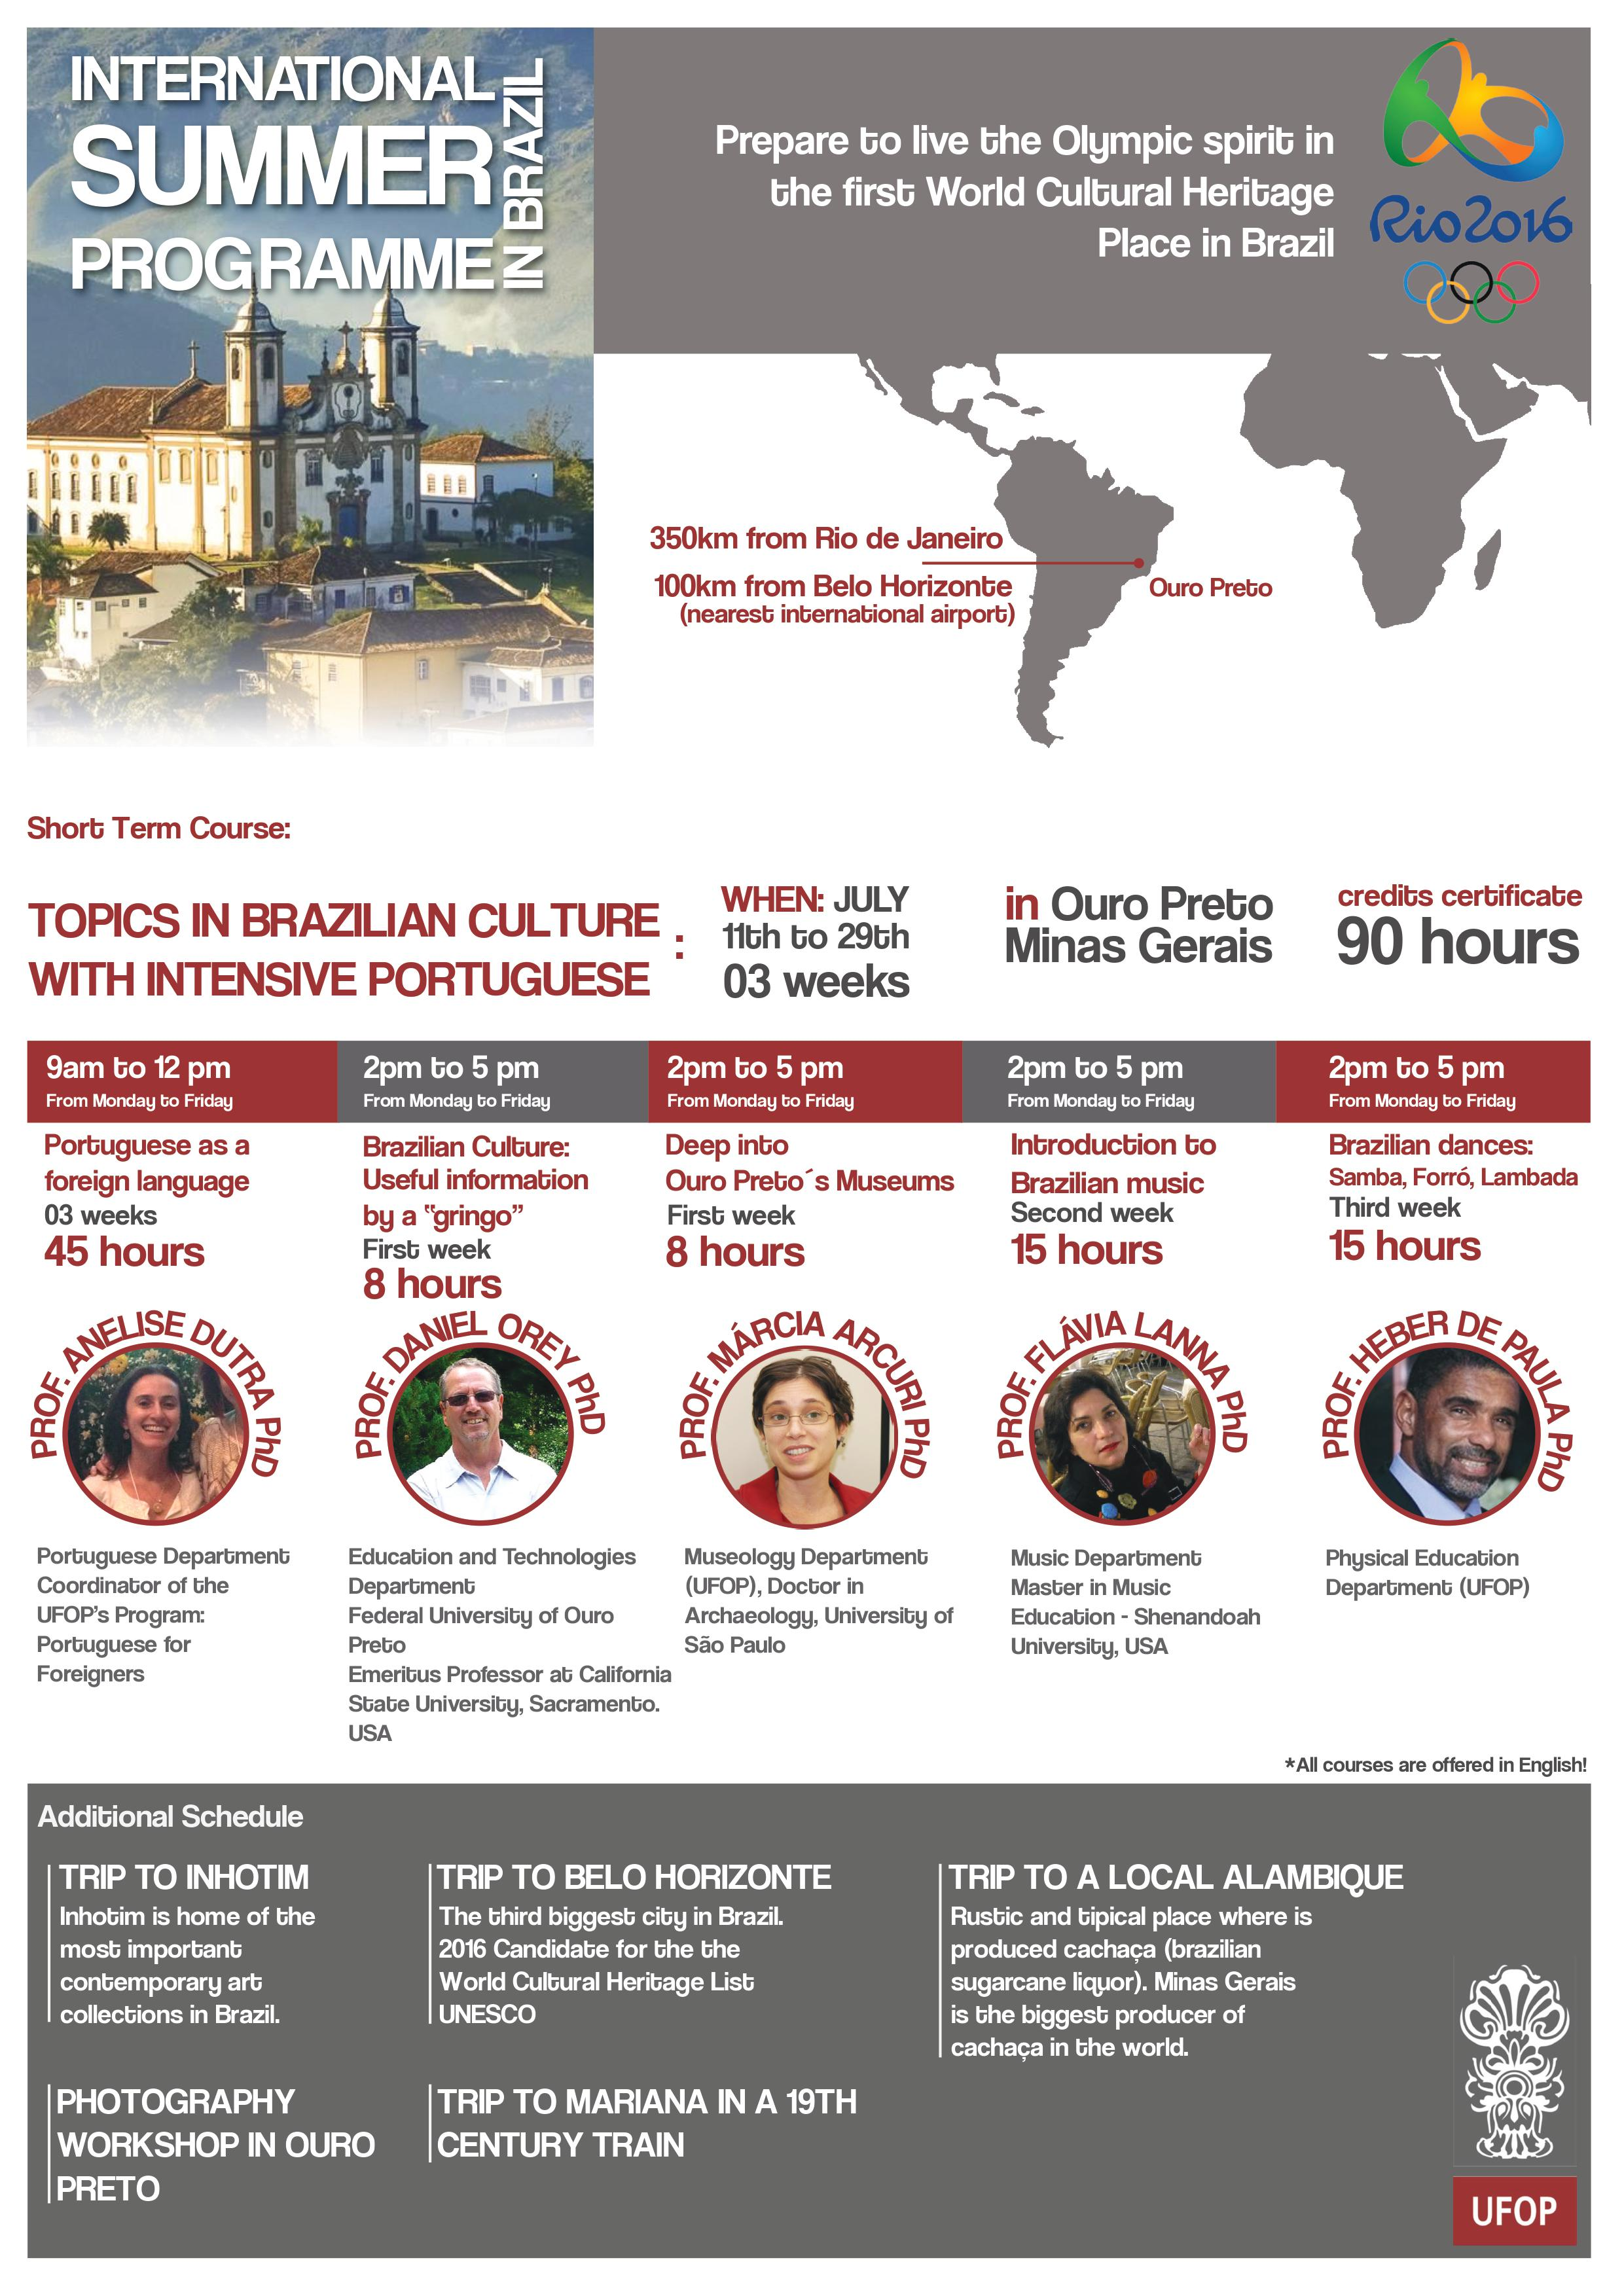
\includegraphics[scale=0.5]{figuras/Summer_Course1.jpg}
	\caption{Primeiro programa de recepção de alunos estrangeiros.}
	\label{fig:01}
\end{figure}
%
\section{Realidade regional e do aluno na UFOP}
%
Em uma estrutura \textit{multicampi}, formada pelos \textit{campi} de Ouro Preto, Mariana e João Monlevade, a universidade está inserida na mesorregião de Belo Horizonte, estendendo-se até João Monlevade, e na microrregião de Ouro Preto, que abrange as cidades de Itabirito, Ouro Preto, Mariana, Diogo de Vasconcelos e Acaiaca. Essa microrregião abarca, conforme dados do censo de $2015$, uma população de aproximadamente $180$ mil habitantes, $193$ unidades escolares estaduais e municipais, uma universidade, um instituto federal e $37$ escolas da rede privada de ensino, com um público escolar de cerca de $5$ mil profissionais da educação e $52$ mil alunos, o que demanda da UFOP uma importante inserção acadêmica e reconhecimento na região \cite{resolucao-cuni-1}.
%
\begin{comment}
A cidade histórica de Ouro Preto é famosa por sua arquitetura colonial e pelo clima peculiar, que dá um charme especial à cidade. Situada a uma altitude média de $1.179$ metros, abriga uma população de mais de $70.000$ habitantes, conforme o censo de $2010$ do Instituto Brasileiro de Geografia e Estatística (IBGE). Com mais de 300 anos de história, Ouro Preto é um dos principais símbolos de Minas Gerais, e não só entre os limites do país, mas também no exterior. A antiga Vila Rica, no passado berço de alguns dos mais importantes movimentos na luta pela independência brasileira e hoje palco de grandiosos eventos culturais, é um dos ícones máximos do Barroco nacional e mundial. A cidade, tombada como Patrimônio Histórico e Cultural da Humanidade, título conferido pela Unesco, é berço de escritores, artistas e toda sorte de personalidades. Mas sobretudo, Ouro Preto é conhecida por ser uma cidade eminentemente universitária.
\end{comment}

Os estudantes da UFOP procedem principalmente dos estados de Minas Gerais, São Paulo, Rio de Janeiro, Espírito Santo e Goiás. Uma realidade que foi sendo alterada gradativamente ao longo dos últimos $15$ anos, período em que a universidade aderiu às novas formas de gestão da educação por parte do governo federal.\footnote{Destaca-se, neste cenário, a alteração do tradicional ``vestibular'' para o Sistema de Seleção Unificada (Sisu), do ministério da educação, em que  as instituições públicas de educação superior oferecem vagas a candidatos participantes do Exame Nacional do Ensino Médio (Enem). Este exame, aliás, foi inspirado nos sistemas utilizados por outros países, como o SAT norte-americano, o Baccalauréat francês e o Gāo Kǎo chinês. O ENEM é considerado o segundo maior exame do gênero no mundo, só sendo superado pelo exame aplicado na China.} Excetuando-se os alunos provindos das escolas federais, percebeu-se um aumento significativo de egressos das escolas públicas da chamada ``região dos Inconfidentes''(Ouro Preto, Mariana e arredores), sobretudo aqueles de Escolas públicas estaduais, que eram raros há alguns anos atrás, especialmente aqueles advindos de classes sociais menos favorecidas. Isto não significa, entretanto, que a realidade da educação pública, sob a ótica do ensino médio, tenha se alterado de forma que o acesso à universidade pública fosse facilitado.

E viver como estudante em Ouro Preto significa, quase sempre, a sua integração em uma das marcas da cultura universitária da cidade: as ``repúblicas estudantis'', que são um tópico à parte.

As repúblicas fazem parte da tradição da cidade. Muitas delas instaladas em prédios históricos, pertencentes à Universidade Federal de Ouro Preto (sendo simplesmente denominadas como ``Repúblicas Federais''), absorvem parcela significativa dos estudantes, tanto em Ouro Preto quanto Mariana. São administradas pelos próprios estudantes, que definem suas regras de admissão. Ao longo de mais de um século, as repúblicas desenvolveram uma cultura própria e mantêm laços estreitos com ex-alunos e ex-residentes, inclusive no que tange à rede de contatos profissionais. Esse laço é muito forte entre as repúblicas federais e mesmo entre as chamadas ``repúblicas particulares'' (que não pertencem à universidade), especialmente na condução das famosas e tradicionais ``festas republicanas'': 12 de outubro, aniversário da Escola de Minas e o 21 de abril, dia de Tiradentes e aniversário das Repúblicas do Campus. Nestes períodos, os antigos ex-alunos costumam marcar presença como uma forma de relembrar e reviver as lembranças dos tempos de universidade. A Refop (Associação das Repúblicas Federais de Ouro Preto) é composta por $67$ repúblicas, sendo uma mista, $51$ masculinas e $15$ femininas. Os alunos veteranos e muitos ex-alunos atestam que a estrutura que existe entre os moradores de uma república são fundamentais para a sua formação como futuros profissionais, especialmente em um contexto de mundo globalizado.
%
\chapter{A gradua{\c c}{\~a}o em Engenharia de Controle e Automa{\c c}{\~a}o}
As atuais demandas da sociedade por bens e servi{\c c}os t{\^e}m sido cada vez mais atendidas utilizando-se de novas tecnologias, resultantes da aplica{\c c}{\~a}o do conhecimento cient{\'i}fico. E isto não é diferente no microclima da região dos inconfidentes, principal ``cliente'' da universidade.

O ensino de engenharia em face dessa realidade passa por grandes mudan{\c c}as, com a cria{\c c}{\~a}o de novas habilita{\c c}{\~o}es, a concep{\c c}{\~a}o e adaptação de novos curr{\'i}culos e estrat{\'e}gias pedag{\'o}gicas, com o objetivo de formar engenheiros capazes de desenvolver, aperfei{\c c}oar e utilizar as novas tecnologias de base cient{\'i}fica.
 
Com o grande desenvolvimento da eletr{\^o}nica, da inform{\'a}tica e das comunicações nas últimas d{\'e}cadas, uma das {\'a}reas mais ativas da engenharia em todo mundo passou a ser, obviamente, a {\'a}rea de Controle e Automa{\c c}{\~a}o.

\section{A importância da Engenharia de Controle e Automa{\c c}{\~a}o}
\label{sec:controleeautomacao}
A hist{\'o}ria do ramo no Brasil data de $1953$, quando o Instituto Tecnol{\'o}gico de Aeron{\'a}utica (ITA) ministrou, pela primeira vez, um curso de controle autom{\'a}tico. Desde ent{\~a}o, a {\'a}rea de Autom{\'a}tica $-$ termo criado para designar a ci{\^e}ncia e a Engenharia de Controle e Automa{\c c}{\~a}o no Brasil$-$ desenvolveu-se rapidamente nas universidades brasileiras, destacando-se os cursos de controle de sistemas din{\^a}micos da USP e Unicamp, j{\'a} no in{\'i}cio dos anos $1970$. 

Atualmente, existem cursos de engenharia associados a sistemas mecatr{\^o}nicos nos Estados Unidos, no Canad{\'a}, na Europa e na {\'A}sia. Ciente da necessidade e da relev{\^a}ncia de se formar engenheiros de Controle e Automa{\c c}{\~a}o no Brasil, o Minist{\'e}rio da Educa{\c c}{\~a}o, atrav{\'e}s da Portaria $1.694$, de $5$ de dezembro de $1994$, publicada no Di{\'a}rio Oficial da Uni{\~a}o de $12$ de dezembro de $1994$, considerando o consubstanciado no parecer da Comiss{\~a}o de Especialistas do Ensino de Engenharia da Secretaria de Educa{\c c}{\~a}o Superior, regulamentou a Engenharia de Controle e Automa{\c c}{\~a}o.

Diversas universidades brasileiras oferecem cursos associados a sistemas mecatr{\^o}nicos, como os cursos oferecidos pela Escola Polit{\'e}cnica da Universidade de S{\~a}o Paulo, o curso de Engenharia de Controle e Automa{\c c}{\~a}o da Universidade Estadual de Campinas, o curso de Engenharia Mec{\^a}nica com {\^e}nfase em Automa{\c c}{\~a}o e Sistemas da Escola de Engenharia de S{\~a}o Carlos da Universidade de S{\~a}o Paulo, o curso de Engenharia de Controle e Automa{\c c}{\~a}o da Universidade Federal de Santa Catarina, o curso de Engenharia de Controle e Automa{\c c}{\~a}o da Universidade Federal de Minas Gerais, o curso de Engenharia Mec{\^a}nica com {\^e}nfase em Mecatr{\^o}nica e o curso de Engenharia de Controle e Automa{\c c}{\~a}o da Pontif{\'i}cia Universidade Católica de Minas Gerais, o curso de Engenharia de Controle e Automa{\c c}{\~a}o da Universidade de Bras{\'i}lia e o curso de Engenharia de Controle e Automa{\c c}{\~a}o da Universidade Federal de Itajub{\'a}.

Na Universidade Federal de Ouro Preto, o curso de Engenharia de Controle e Automa{\c c}{\~a}o foi concebido no final da d{\'e}cada de $1990$ de forma a responder às necessidade de expans{\~a}o da pr{\'o}pria institui{\c c}{\~a}o (e tamb{\'e}m do mercado), face aos novos tempos. Sabia-se, at{\'e} aquele momento, que a universidade possu{\'i}a contribui{\c c}{\~o}es significativas para o desenvolvimento da engenharia no Brasil, especialmente pela tradi{\c c}{\~a}o centen{\'a}ria da Escola de Minas. Assim, em agosto do ano $2000$, iniciam-se as primeiras turmas do curso de gradua{\c c}{\~a}o em Engenharia de Controle e Automa{\c c}{\~a}o na UFOP. Vale mais uma vez ressaltar que o curso foi o campeão de inscrições na universidade, quando aberto o primeiro vestibular.

Sob a ótica industrial, não é desproposital afirmar que há, ainda, escassez de profissionais com essa formação no país. Segundo informações do guia do estudante de $2016$ \cite{guia-do-estudante}, os setores de petróleo e gás, manufatura, mineração e metalurgia são tradicionais empregadores. Três novas áreas apresentam grande potencial: indústria portuária, robótica e a domótica (pesquisa e desenvolvimento de automação de rotinas e tarefas domésticas). Empresas automobilísticas também demandam o graduado. O Sul, o Sudeste e a região da Zona Franca de Manaus são os principais centros de emprego ao longo do país. Na região de maior atuação da universidade federal de Ouro Preto, os grandes empregadores são as empresas de mineração, metalurgia e as de base tecnológica situadas na região metropolitana de Belo Horizonte. 

Pode-se inclusive, ressaltar a crescente importância da Engenharia de Controle e Automação para as áreas de:
\begin{itemize}
\item conservação do patrimônio histórico, especialmente na área de conforto térmico: controle de temperatura, umidade e iluminação;
\item iluminação pública;
\item automação comercial e predial;
\item pesquisa e desenvolvimento de tecnologias assistivas para portadores de necessidades especiais: visão, motora e intelectual;
\item automação agrária.
\end{itemize}

Desde a criação da graduação em Engenharia de Controle e Automação, que comemora seus quase $16$ anos de história, poucas alterações haviam ocorrido em seu arcabouço. E isto vai de encontro a um mundo que se alterou rapidamente, em termos científicos, econômicos e tecnológicos no mesmo período.

Após a divulgação, por parte da pró-reitoria de graduação da UFOP de um programa de restruturação chamado Plano de Ações Pedagógicas (PAP) em $2014$, surgiu a necessidade de se rediscutir toda a base da graduação em Engenharia de Controle e Automação. E isto passa pela rescrita de todo o projeto de curso e não apenas sua atualização.

\section[O PPC]{O projeto pedag{\'o}gico de curso} \label{sec:ocurso}
%
A principal proposta do Projeto Pedagógico de Curso ou, simplesmente, PPC\footnote{Podendo ser chamado também de Projeto Político e Pedagógico, PPP.} {\'e} a de envolver discentes, docentes e t{\'e}cnicos administrativos, no contexto do curso de engenharia de controle e automa{\c c}{\~a}o, para conscientiza{\c c}{\~a}o  e participa{\c c}{\~a}o ativa frente aos desafios a serem superados, que culminem na restrutura{\c c}{\~a}o e aperfei{\c c}oamento da graduação como um todo. Entende-se que este n{\~a}o deve ser mais um documento, mas um horizonte norteador que se prop{\~o}e a direcionar o trabalhos e a vis{\~a}o de toda a comunidade acad{\^e}mica. 

No primeiro ciclo de debates, promovidos pelo N{\'u}cleo Docente Estruturante (NDE) em parceria com o colegiado de curso (CECAU), foram levantadas diversas propostas para a melhoria cont{\'i}nua, seguindo a filosofia proposta pela PROGRAD, em conson{\^a}ncia com o projeto de desenvolvimento institucional da Universidade Federal de Ouro Preto (PDI-UFOP). A ideia geral foi a de elaborar a{\c c}{\~o}es de car{\'a}cter mais espec{\'i}fico, que repercurtir{\~a}o em curto, m{\'e}dio e longo prazos.

O consenso geral foi a necessidade de consolidar a gradua{\c c}{\~a}o em engenharia de controle e automa{\c c}{\~a}o, por interm{\'e}dio da atualiza{\c c}{\~a}o em seu projeto pedag{\'o}gico (PPC), especialmente ap{\'o}s a chegada de novos docentes e o aumento (de $100\%$) na oferta de vagas para alunos ingressantes a cada ano, ap{\'o}s o programa de restrutura{\c c}{\~a}o das universidades fererais, o Reuni. 

Tomou-se ent{\~a}o como principais desafios para restrutura{\c c}{\~a}o do PPC a atualiza{\c c}{\~a}o da matriz curricular, com a revis{\~a}o de programas de disciplinas, identifica{\c c}{\~a}o e diminui{\c c}{\~a}o do d{\'e}ficit de bibliografias, elabora{\c c}{\~a}o de regras internas para a capacita{\c c}{\~a}o de docentes, cria{\c c}{\~a}o de material instituicional de divulga{\c c}{\~a}o, inser{\c c}{\~a}o de calouros e envolvimento de veteranos em estudos de novas pr{\'a}ticas pedag{\'o}gicas, como a ``aprendizagem ativa'', o aumento no n{\'u}mero de bolsas de monitoria e at{\'e} mesmo quest{\~o}es relativas {\`a} infra-estrutura de laborat{\'o}rios, que seguramente repercutir{\~a}o na qualidade do ensino e na diminui{\c c}{\~a}o das taxas de evas{\~a}o do curso.
%\chapter{Concepção do Curso}

\section{Dados de identificação do curso}

\section{Objetivos e perfil do egresso} \label{sec:perfildoegresso}

Poder-se-ia dizer que a forma{\c c}{\~a}o do engenheiro de controle e automa{\c c}{\~a}o encerra um car{\'a}ter abrangente de atua{\c c}{\~a}o na natureza e, por este motivo,  tem como pedra fundamental a integra{\c c}{\~a}o entre diversas {\'a}reas do conhecimento humano, desde a matem{\'a}tica, f{\'i}sica, qu{\'i}mica e ci{\^e}ncias da computa{\c c}{\~a}o. No entanto, sua atua{\c c}{\~a}o n{\~a}o se restringe a tais campos do saber, podendo dar-se em inumer{\'a}veis outros campos, o que torna dif{\'i}cil a tarefa de enquadr{\'a}-lo nas tradicionais {\'a}reas da engenharia, como el{\'e}trica, eletr{\^o}nica, mec{\^a}nica ou computa{\c c}{\~a}o.

Os departamentos de Matem{\'a}tica, F{\'i}sica, Computa{\c c}{\~a}o, Controle e Automa{\c c}{\~a}o e T{\'e}cnicas Fundamentais(necessita de revis{\~a}o para incluir a Mec{\^a}nica), Metalurgia e de Materiais, Minas e Produ{\c c}{\~a}o disp{\~o}em de recursos humanos, instala{\c c}{\~o}es e desenvolvem atividades de ensino e de pesquisa de alto n{\'i}vel nas {\'a}reas de Ci{\^e}ncias Exatas, Ci{\^e}ncias da Engenharia e Processos Industriais em Minera{\c c}{\~a}o e Metalurgia. 

Al{\'e}m disso, o Departamento de Computa{\c c}{\~a}o desenvolve atividades de ensino e de pesquisa em todas as {\'a}reas de forma{\c c}{\~a}o profissional da Engenharia de Controle e Automa{\c c}{\~a}o ligadas a software e o Departamento de Engenharia de Controle e Automa{\c c}{\~a}o e T{\'e}cnicas Fundamentais(necessita de revis{\~a}o para incluir a Mec{\^a}nica) tem um núcleo consolidado que desenvolve ensino e pesquisa tecnológica em todas as {\'a}reas de forma{\c c}{\~a}o profissional ligadas a hardware do Curso de Engenharia de Controle e Automa{\c c}{\~a}o.

Portanto, as necessidades de investimento em recursos materiais e na contrata{\c c}{\~a}o de novos profissionais para a implanta{\c c}{\~a}o do Curso de Engenharia de Controle e Automa{\c c}{\~a}o na UFOP s{\~a}o complementares e relativamente pequenas, ficando demonstrada a viabilidade de um Curso de Engenharia de Controle e Automa{\c c}{\~a}o na UFOP.
 

\section{Situa{\c c}{\~a}o atual e desafios}

Pode-se afirmar que, desde a cria{\c c}{\~a}o do curso de eng. de controle e automa{\c c}{\~a}o em $1999$, muitos desafios foram superados. Identificou-se como sendo um dos principais focos dados para o curso at{\'e} ent{\~a}o, especialmente no que concerne ao perfil dos egressos, o da forma{\c c}{\~a}o espec{\'i}fica para a atua{\c c}{\~a}o em empresas, destacando-se aquelas do setor m{\'i}nero-metal{\'u}rgico. Tal justificativa dava-se pela voca{\c c}{\~a}o da pr{\'o}pria regi{\~a}o e necessidades do mercado. No entanto, passada mais de uma d{\'e}cada de sua exist{\^e}ncia, detectamos a necessidade de expans{\~a}o de conceitos, de forma a contribuir na forma{\c c}{\~a}o de engenheiros com perfil mais abrangente e empreendedor, dentro de uma perspectiva hol{\'i}stica, {\'e}tica e humanista, e n{\~a}o apenas para suprir demandas mercadol{\'o}gicas.



%A partir de tais discuss{\~o}es, o primeiro plano de a{\c c}{\~o}es para o curso de Engenharia de Controle e Automa{\c c}{\~a}o foi elaborado e sumarizado na planilha anexa
\chapter{Administra{\c c}{\~a}o Acad{{\^e}mica}}
\label{cap:03} \index{administracao}

\section{Coordenação Acadêmica}
Segundo o Estatuto e Regimento da Universidade Federal de Ouro Preto-UFOP, de $1999$ (Artigo $23$, $ 1^{\circ}$  parágrafo), ``os Colegiados de Cursos são as instâncias universitárias responsáveis pela coordenação didática das disciplinas constituintes do projeto pedagógico de cada curso''.

A coordenação acadêmica do curso de Engenharia de Controle e Automação é exercida pelo Colegiado de Curso de Engenharia de Controle e Automação – CECAU, que é presidido pelo coordenador do curso, cuja composição e atribuições cumprem o que determina o Estatuto (Resolução CUNI nº 414 – atualizada em 28 de agosto de 2014)(anexo \ref{ape:02}) e o Regimento Geral (Resolução CUNI nº 435 – atualizada em 22 de dezembro de 2014) da Universidade Federal de Ouro Preto, conforme a Portaria nº 1.486, de 29 de dezembro de 1998, publicado, no Diário Oficial da União de 30 de dezembro de 1998, seção I, página 12. 

A coordenação acadêmica do Curso de Engenharia de Controle e Automação será exercida pelo Colegiado de Engenharia de Controle e Automação, que é presidido pelo coordenador do curso. Como órgão deliberativo, cabe ao colegiado avaliar o Projeto Político e Pedagógico, que é elaborado pelo Núcleo Docente Estruturante (NDE) e estabelecer as normas para a orientação acadêmica:

\textbf{CECAU - Colegiado do Curso de Engenharia de Controle e Automação}

Presidente: Prof. Agnaldo José da Rocha Reis

E-mail: agnreis@gmail.com

Secretária: Rosilene Pedrosa Gomes

Telefone: 3559-1542

E-mail: col.ufop@gmail.com

Além das atividades inerentes à coordenação acadêmica e didática das disciplinas constituintes do projeto pedagógico do curso, o Presidente do Colegiado do Curso de Engenharia de Controle \& Automação, além de outros setores da Universidade, deverá manter contatos com empresas, institutos de pesquisa, repartições públicas, etc. com o objetivo de estabelecer os convênios para realização de estágios, pesquisa, monitoria e extensão a serem realizados pelos alunos do curso.

\section{Atribuições do colegiado de curso}
O Artigo $25$ do atual Estatuto e Regimento vigente estabelece que os colegiados de curso da UFOP têm as seguintes atribuições:
\begin{enumerate}
	\item Compatibilizar as diretrizes gerais dos programas das disciplinas do respectivo curso e determinar aos departamentos as modificações necessárias;
	
	\item Integrar os planos elaborados pelos departamentos, relativos ao ensino das várias disciplinas, para fim de organização do programa didático do curso;
	
	\item Recomendar ao departamento, a que esteja vinculada a disciplina, as providências adequadas à melhor utilização das instalações, do material e do aproveitamento do pessoal;
	
	\item Propor a aprovação do Conselho de Ensino Pesquisa e Extensão o currículo pleno do curso e suas alterações, com indicação dos pré-requisitos, da carga horária, das ementas, dos programas e dos créditos das disciplinas que o compõem;
	
	\item Decidir sobre questões relativas a reopção de cursos, equivalência de disciplinas, jubilamento, matrícula em disciplinas isoladas e transferência;
	
	\item Apreciar as recomendações dos departamentos e requirimentos dos doscentes sobre assunto de interesse do curso;
	
	\item Exercer atividades de orientação acadêmica dos estudantes do curso, com vistas ao cumprimento dos créditos necessários à candidatura à colação de grau;
	
	\item Indicar para a Pró-Reitoria de Graduação os candidatos à colação de grau.
\end{enumerate}

\textbf{COARQ - Colegiado do Curso de Arquitetura e Urbanismo}

Presidente: Profª. Sandra Maria Antunes Nogueira

E-mail: sandramnog@gmail.com

Secretária: Naiara Pinheiro de Castilho

Telefone: 3559-1542

E-mail: colegiados.em@gmail.com



\textbf{CEAMB - Colegiado do Curso de Engenharia Ambiental}

Presidente: Prof. Gilberto Queiroz da Silva

E-mail: gqueiroz@em.ufop.br

Secretária: Marilene Guimarães Bretas

Telefone: 3559-1542

E-mail: ceamb@em.ufop.br



\textbf{CECIV - Colegiado do Curso de Engenharia de Civil}

Presidente: Prof. Geraldo Donizetti de Paula

E-mail: gdepaula9@gmail.com

Secretária: Marilene Guimarães Bretas

Telefone: 3559-1542

E-mail: ceciv@em.ufop.br



\textbf{CECAU - Colegiado do Curso de Engenharia de Controle e Automação}

Presidente: Prof. Agnaldo José da Rocha Reis

E-mail: agnreis@gmail.com

Secretária: Rosilene Pedrosa Gomes

Telefone: 3559-1542

E-mail: col.ufop@gmail.com



\textbf{CEGEO - Colegiado do Curso de Engenharia Geológica}

Presidente: Prof. Marco Antônio Fonseca

E-mail: marco@degeo.ufop.br

Secretária: Rosilene Pedrosa Gomes

Telefone: 3559-1542

E-mail: col.ufop@gmail.com



\textbf{CEMEC - Colegiado do Curso de Engenharia Mecânica}

Presidente: Prof. Luis Antônio Bortolaia

E-mail: luis.bortolaia@em.ufop.br

Secretária: Naiara Pinheiro de Castilho

Telefone: 3559-1542

E-mail: colegiados.em@gmail.com


\textbf{CEMET - Colegiado do Curso de Engenharia Metalúrgica}

Presidente: Prof. Luiz Cláudio Cândido

E-mail: candido@em.ufop.br

Secretária: Naiara Pinheiro de Castilho

Telefone: 3559-1542

E-mail: colegiados.em@gmail.com


\textbf{CEMIN - Colegiado do Curso de Engenharia de Minas}

Presidente: Prof. Carlos Alberto Pereira

E-mail: pereiraufop@gmail.com

Secretária: Marilene Guimarães Bretas

Telefone: 3559-1542

E-mail: cemin@em.ufop.br


\textbf{CEPRO - Colegiado do Curso de Engenharia de Produção}

Presidente: Profª. Francisca Diana Ferreira

E-mail: dianaufu@yahoo.com.br

Secretária: Rosilene Pedrosa Gomes

Telefone: 3559-1542

E-mail: col.ufop@gmail.com

\section{Núcleo Docente Estruturante}

O Núcleo Docente Estruturante foi um conceito criado pela portaria $N^{\circ 147}$ de $2$ de fevereiro de $2007$, com o intuito de qualificar o envolvimento docente no processo de concepção e consolidação de um curso de graduação:
\begin{citacao}
	``Entende-se, então, que todo curso que tem qualidade possui (ainda que informalmente) um grupo de professores que, poder-se-ia  dizer,  é a alma do curso. Em  outras palavras, trata-se de um núcleo docente estruturante.	É importante ainda observar que, dentro da tradição bastante  burocratizante  das instituições de ensino no Brasil, recomendar-se ou, mais ainda, exigir-se a existência de um NDE, tenderia a induzir a definição deste como um 
	órgão deliberativo, o que pode significar a perda da eficácia de suas funções. O NDE  deve ser considerado não como  exigência ou requisito legal, mas como elemento diferenciador da qualidade do curso, no que diz respeito à interseção entre as dimensões do corpo docente e Projeto Pedagógico do Curso.''
\end{citacao}

Na UFOP, o NDE foi estabelecido segundo a Resolução xxxx, sendo constituído pelo(a) Coordenador(a) de Curso (presidente de colegiado), como membro e por pelo menos $30\%$ (trinta por cento) dos docentes efetivos e atuantes no curso, relacionados pelo Colegiado de Curso que satisfizerem os requisitos previstos na resolução. Um dos professores é escolhido para presidir o núcleo, desde que o mesmo não seja o coordenador do curso.
 
Ao NDE cabe a manutenção do presente Projeto Pedagógico de Curso (PPC) e a correspondente implementação. O NDE é um órgão consultivo, cujas sugestões e decorrentes ações devem ser avaliadas e aprovadas pelo Colegiado de Curso de Engenharia de Controle e Automação, que é o órgão deliberativo. 

Este grupo deve avaliar constantemente o andamento do Curso, especialmente nos primeiros anos, propondo melhorias e ajustes no PPC que impactem no bom funcionamento do Curso, de forma a possibilitar a realização dos objetivos propostos.

\section{Corpo Docente}
O corpo docente pode ser consultado a partir da tabela \ref{tab:0301}.

% Please add the following required packages to your document preamble:
% \usepackage{graphicx}
% \usepackage[table,xcdraw]{xcolor}
% If you use beamer only pass "xcolor=table" option, i.e. \documentclass[xcolor=table]{beamer}
\begin{table}[p]
		\caption{Corpo Docente - Engenharia de Controle \& Automação e Engenharia Mecânica.}
		\label{tab:0301}
	\resizebox{\textwidth}{!}{%
		\begin{tabular}{@{}lllll@{}}
			\toprule
			\multicolumn{1}{c}{{\color[HTML]{3531FF} \textbf{Nome}}}                               & \multicolumn{1}{c}{{\color[HTML]{3531FF} \textbf{Título}}} & \multicolumn{1}{c}{{\color[HTML]{3531FF} \textbf{Área}}} & \multicolumn{1}{c}{{\color[HTML]{3531FF} \textbf{Sub-Área}}}                                                                                                                                                                                                                                          & \multicolumn{1}{c}{{\color[HTML]{3531FF} \textbf{Contato}}}    \\ \midrule
			\multicolumn{1}{|l|}{{\color[HTML]{3531FF} \textbf{Adrielle de Carvalho Santana}}}     & \multicolumn{1}{l|}{Doutoranda}                            & \multicolumn{1}{l|}{Controle e Automação}                & \multicolumn{1}{l|}{\begin{tabular}[c]{@{}l@{}}Sistemas eletrônicos de Medida e Controle\\ Medição, Controle, Correção e Proteção \\ de Sistemas Elétricos de Potência\\ Eletrônica Industrial, Sistemas e Controles Eletrônicos\\ Controle de Processos Eletrônicos, Retroalimentação.\end{tabular}} & \multicolumn{1}{l|}{}                                          \\ \midrule
			\multicolumn{1}{|l|}{{\color[HTML]{3531FF} \textbf{Agnaldo Jose da Rocha Reis}}}       & \multicolumn{1}{l|}{Doutor}                                & \multicolumn{1}{l|}{Controle e Automação}                & \multicolumn{1}{l|}{\begin{tabular}[c]{@{}l@{}}Instrumentação,\\ Interfaceamento de sistemas\\ Laboratórios de Controle e Automação\\ Identificação de Sistemas.\end{tabular}}                                                                                                                        & \multicolumn{1}{l|}{}                                          \\ \midrule
			\multicolumn{1}{|l|}{{\color[HTML]{3531FF} \textbf{Alan Kardek Rego Segundo}}}         & \multicolumn{1}{l|}{Doutor}                                & \multicolumn{1}{l|}{Controle e Automação}                & \multicolumn{1}{l|}{\begin{tabular}[c]{@{}l@{}}Sistemas eletrônicos de Medida e Controle \\ Controle de Processos Eletrônicos,\\ Retroalimentação\\ Instrumentação eletrônica.\end{tabular}}                                                                                                          & \multicolumn{1}{l|}{}                                          \\ \midrule
			\multicolumn{1}{|l|}{{\color[HTML]{3531FF} \textbf{Antonio Maria Claret de Gouveia}}}  & \multicolumn{1}{l|}{Doutor}                                & \multicolumn{1}{l|}{Mecânica}                            & \multicolumn{1}{l|}{}                                                                                                                                                                                                                                                                                 & \multicolumn{1}{l|}{}                                          \\ \midrule
			\multicolumn{1}{|l|}{{\color[HTML]{3531FF} \textbf{Danny Augusto Vieira Tonidandel}}}  & \multicolumn{1}{l|}{Doutorando}                            & \multicolumn{1}{l|}{Controle e Automação}                & \multicolumn{1}{l|}{\begin{tabular}[c]{@{}l@{}}História da Engenharia Elétrica\\ História da Ciência\\ Automação eletrônica de				Processos Elétricos e Industriais.\end{tabular}}                                                                                                                    & \multicolumn{1}{l|}{\url{http://professor.ufop.br/tonidandel}} \\ \midrule
			\multicolumn{1}{|l|}{{\color[HTML]{3531FF} \textbf{Diogo Antonio de Sousa}}}           & \multicolumn{1}{l|}{Mestre}                                & \multicolumn{1}{l|}{Mecânica}                            & \multicolumn{1}{l|}{\begin{tabular}[c]{@{}l@{}}Projetos de Máquinas\\ Elementos de máquinas\\ Máquinas de Usinagem e Conformação.\end{tabular}}                                                                                                                                                       & \multicolumn{1}{l|}{}                                          \\ \midrule
			\multicolumn{1}{|l|}{{\color[HTML]{3531FF} \textbf{Eliana Ferreira Rodrigues}}}        & \multicolumn{1}{l|}{Doutor}                                & \multicolumn{1}{l|}{Mecânica}                            & \multicolumn{1}{l|}{}                                                                                                                                                                                                                                                                                 & \multicolumn{1}{l|}{}                                          \\ \midrule
			\multicolumn{1}{|l|}{{\color[HTML]{3531FF} \textbf{Elisângela Martins Leal}}}          & \multicolumn{1}{l|}{Doutor}                                & \multicolumn{1}{l|}{Mecânica}                            & \multicolumn{1}{l|}{\begin{tabular}[c]{@{}l@{}}Aproveitamento de Energia\\ Geração de Energia\\ Elétrica\\ Balanços Globais de Matéria e Energia.\end{tabular}}                                                                                                                                       & \multicolumn{1}{l|}{}                                          \\ \midrule
			\multicolumn{1}{|l|}{{\color[HTML]{3531FF} \textbf{Gustavo Paulinelli Guimarães}}}     & \multicolumn{1}{l|}{Doutor}                                & \multicolumn{1}{l|}{Mecânica}                            & \multicolumn{1}{l|}{\begin{tabular}[c]{@{}l@{}}Máquinas, Motores e Equipamentos\\ Estática e Dinâmica Aplicada\end{tabular}}                                                                                                                                                                          & \multicolumn{1}{l|}{}                                          \\ \midrule
			\multicolumn{1}{|l|}{{\color[HTML]{3531FF} \textbf{Henor Artur de Souza}}}             & \multicolumn{1}{l|}{Doutor}                                & \multicolumn{1}{l|}{Mecânica}                            & \multicolumn{1}{l|}{}                                                                                                                                                                                                                                                                                 & \multicolumn{1}{l|}{}                                          \\ \midrule
			\multicolumn{1}{|l|}{{\color[HTML]{3531FF} \textbf{Igor Cézar Pereira}}}               & \multicolumn{1}{l|}{Doutor}                                & \multicolumn{1}{l|}{Mecânica}                            & \multicolumn{1}{l|}{\begin{tabular}[c]{@{}l@{}}Processos de Fabricação\\ Processo de Fabricação por Fundição\\ Processo de Fabricação por Soldagem.\end{tabular}}                                                                                                                                     & \multicolumn{1}{l|}{}                                          \\ \midrule
			\multicolumn{1}{|l|}{{\color[HTML]{3531FF} \textbf{João Carlos Vilela de Castro}}}     & \multicolumn{1}{l|}{Mestre}                                & \multicolumn{1}{l|}{Controle e Automação}                & \multicolumn{1}{l|}{Robótica}                                                                                                                                                                                                                                                                         & \multicolumn{1}{l|}{}                                          \\ \midrule
			\multicolumn{1}{|l|}{{\color[HTML]{3531FF} \textbf{José Alberto Naves Cocota Junior}}} & \multicolumn{1}{l|}{Doutorando}                            & \multicolumn{1}{l|}{Controle e Automação}                & \multicolumn{1}{l|}{\begin{tabular}[c]{@{}l@{}}Sistemas eletrônicos de medida e controle\\ Controle de Processos Eletrônicos, Retroalimentação\\ Instrumentação eletrônica.\end{tabular}}                                                                                                             & \multicolumn{1}{l|}{}                                          \\ \midrule
			\multicolumn{1}{|l|}{{\color[HTML]{3531FF} \textbf{Karla Boaventura P. Palmieri}}}     & \multicolumn{1}{l|}{Doutor}                                & \multicolumn{1}{l|}{Controle e Automação}                & \multicolumn{1}{l|}{\begin{tabular}[c]{@{}l@{}}Informática Industrial\\ Sistemas Integrados de Manufatura\end{tabular}}                                                                                                                                                                               & \multicolumn{1}{l|}{}                                          \\ \midrule
			\multicolumn{1}{|l|}{{\color[HTML]{3531FF} \textbf{Luciana Gomes Castanheira}}}        & \multicolumn{1}{l|}{Doutoranda}                            & \multicolumn{1}{l|}{Controle e Automação}                & \multicolumn{1}{l|}{Robótica.}                                                                                                                                                                                                                                                                        & \multicolumn{1}{l|}{}                                          \\ \midrule
			\multicolumn{1}{|l|}{{\color[HTML]{3531FF} \textbf{Luís Antônio Bortolaia}}}           & \multicolumn{1}{l|}{Doutor}                                & \multicolumn{1}{l|}{Mecânica}                            & \multicolumn{1}{l|}{Engenharia Térmica.}                                                                                                                                                                                                                                                              & \multicolumn{1}{l|}{}                                          \\ \midrule
			\multicolumn{1}{|l|}{{\color[HTML]{3531FF} \textbf{Luiz Fernando Ríspoli Alves}}}      & \multicolumn{1}{l|}{Doutor}                                & \multicolumn{1}{l|}{Controle e Automação}                & \multicolumn{1}{l|}{Automação Residencial e Predial}                                                                                                                                                                                                                                                  & \multicolumn{1}{l|}{}                                          \\ \midrule
			\multicolumn{1}{|l|}{{\color[HTML]{3531FF} \textbf{Luiz Joaquim Cardoso Rocha}}}       & \multicolumn{1}{l|}{Doutor}                                & \multicolumn{1}{l|}{Mecânica}                            & \multicolumn{1}{l|}{\begin{tabular}[c]{@{}l@{}}Sistemas termodinâmicos\\ Acionamentos Fluidomecânicos.\end{tabular}}                                                                                                                                                                                  & \multicolumn{1}{l|}{}                                          \\ \midrule
			\multicolumn{1}{|l|}{{\color[HTML]{3531FF} \textbf{Margarida Márcia F. Lima}}}         & \multicolumn{1}{l|}{Doutor}                                & \multicolumn{1}{l|}{Mecânica}                            & \multicolumn{1}{l|}{Ciência e Tecnologia de Materiais}                                                                                                                                                                                                                                                & \multicolumn{1}{l|}{}                                          \\ \midrule
			\multicolumn{1}{|l|}{{\color[HTML]{3531FF} \textbf{Milton Realino de Paula}}}          & \multicolumn{1}{l|}{Doutor}                                & \multicolumn{1}{l|}{Mecânica}                            & \multicolumn{1}{l|}{\begin{tabular}[c]{@{}l@{}}Sistemas termodinâmicos\\ Acionamentos Fluidomecânicos.\end{tabular}}                                                                                                                                                                                  & \multicolumn{1}{l|}{}                                          \\ \midrule
			\multicolumn{1}{|l|}{{\color[HTML]{3531FF} \textbf{Paulo Henrique Vieira Magalhães}}}  & \multicolumn{1}{l|}{Doutor}                                & \multicolumn{1}{l|}{Mecânica}                            & \multicolumn{1}{l|}{\begin{tabular}[c]{@{}l@{}}Sistemas mecânicos ou Projetos\\ Processos de Fabricação Mecânica\end{tabular}}                                                                                                                                                                        & \multicolumn{1}{l|}{}                                          \\ \midrule
			\multicolumn{1}{|l|}{{\color[HTML]{3531FF} \textbf{Paulo Marcos de Barros Monteiro}}}  & \multicolumn{1}{l|}{Doutor}                                & \multicolumn{1}{l|}{Controle e Automação}                & \multicolumn{1}{l|}{Sistemas de Controle.}                                                                                                                                                                                                                                                            & \multicolumn{1}{l|}{}                                          \\ \midrule
			\multicolumn{1}{|l|}{{\color[HTML]{3531FF} \textbf{Regiane de Sousa Silva Ramalho}}}   & \multicolumn{1}{l|}{Mestre}                                & \multicolumn{1}{l|}{Controle e Automação}                & \multicolumn{1}{l|}{\begin{tabular}[c]{@{}l@{}}Automação eletrônica de processos\\ elétricos e industriais.\end{tabular}}                                                                                                                                                                             & \multicolumn{1}{l|}{}                                          \\ \midrule
			\multicolumn{1}{|l|}{{\color[HTML]{3531FF} \textbf{Ronilson Rocha}}}                   & \multicolumn{1}{l|}{Doutor}                                & \multicolumn{1}{l|}{Controle e Automação}                & \multicolumn{1}{l|}{\begin{tabular}[c]{@{}l@{}}Sistemas de Automação e Controle\\ Instrumentação.\end{tabular}}                                                                                                                                                                                       & \multicolumn{1}{l|}{}                                          \\ \midrule
			\multicolumn{1}{|l|}{{\color[HTML]{3531FF} \textbf{Sávio Augusto Lopes da Silva}}}     & \multicolumn{1}{l|}{Doutor}                                & \multicolumn{1}{l|}{Controle e Automação}                & \multicolumn{1}{l|}{}                                                                                                                                                                                                                                                                                 & \multicolumn{1}{l|}{}                                          \\ \midrule
			\multicolumn{1}{|l|}{{\color[HTML]{3531FF} \textbf{Sávio Sade Tayer}}}                 & \multicolumn{1}{l|}{Mestre}                                & \multicolumn{1}{l|}{Mecânica}                            & \multicolumn{1}{l|}{\begin{tabular}[c]{@{}l@{}}Projetos de Máquinas\\ Elementos de Máquinas\\ Máquinas de Usinagem e Conformação\end{tabular}}                                                                                                                                                        & \multicolumn{1}{l|}{}                                          \\ \midrule
			\multicolumn{1}{|l|}{{\color[HTML]{3531FF} \textbf{Washington Luis Vieira da Silva}}}  & \multicolumn{1}{l|}{Doutor}                                & \multicolumn{1}{l|}{Mecânica}                            & \multicolumn{1}{l|}{Planejamento e Controle da Produção.}                                                                                                                                                                                                                                             & \multicolumn{1}{l|}{}                                          \\ \midrule
			\multicolumn{1}{|l|}{{\color[HTML]{3531FF} \textbf{Zirlene Alves da Silva Santos}}}    & \multicolumn{1}{l|}{Doutor}                                & \multicolumn{1}{l|}{Mecânica}                            & \multicolumn{1}{l|}{\begin{tabular}[c]{@{}l@{}}Gerência da Qualidade\\ Desenvolvimento de Produto.\end{tabular}}                                                                                                                                                                                      &                                                                \\ \bottomrule
		\end{tabular}%
	}
\end{table}
\chapter{Organização curricular} 
\label{cap:04} \index{curriculo}
%
A organização curricular do curso de graduação em Engenharia de Controle e Automação da Universidade Federal de Ouro Preto, busca seguir as Diretrizes Curriculares Nacionais (DCN) dos Cursos de Engenharia estabelecidas no Parecer CNE/CES 1362/2001\footnote{Publicada no D.O.U. de 25 de Fevereiro de 2002.} bem como a Resolução do Ministério da Educação e do Desporto (MEC) número 48 de 1976 e a Portaria MEC número 1.694 de 05 de dezembro de 1994\footnote{Publicada no D.O.U. de 12 de Dezembro de 1994.}. As disciplinas e atividades presentes na matriz curricular foram organizadas de forma a atender aos objetivos e perfil profissional do egresso, descritos no item 2 deste Projeto Pedagógico de Curso.

A tabela \ref{tab:0401} resume a proposta de organização dos componentes curriculares do curso de Engenharia de Controle e Automação da UFOP.

\begin{table}[htpb]
	\centering
	\caption{Organização de componentes curriculares.}
	\label{tab:0401}
	\resizebox{\textwidth}{!}{%
		\begin{tabular}{|l|l|l|l}
			\cline{1-3}
			\textbf{COMPONENTES CURRICULARES}       & \textbf{QUANTIDADE} & \textbf{CARGA HORÁRIA} &  \\ \cline{1-3}
			Disciplinas Obrigatórias                & 49                  & 2730                   &  \\ \cline{1-3}
			Disciplinas Eletivas                    & -                   & 240                    &  \\ \cline{1-3}
			Estágios                                & 1                   & 160                    &  \\ \cline{1-3}
			Monografia                              & 1                   & 300                    &  \\ \cline{1-3}
			Atividade Acadêmico-Científico-Cultural & -                   & 170                    &  \\ \cline{1-3}
			\textbf{TOTAL}                          & \textbf{51}         & \textbf{3600}          &  \\ \cline{1-3}
		\end{tabular}%
	}
\end{table}

\section{Matriz Curricular} \label{sec:matriz}

A Matriz Curricular do curso de graduação em Engenharia de Controle e Automação da UFOP discrimina os componentes curriculares obrigatórios e complementares. Os componentes obrigatórios são compostos pelas disciplinas, estágio supervisionado e a Monografia. Os componentes complementares são constituídos pelas disciplinas eletivas as quais têm a função de integralizar a formação profissional do aluno com conteúdo na área de Sinais e Sistemas, Automação Industrial e de Formação Geral. O aluno também deverá realizar Atividades Acadêmico-Científico-Cultural (AACC) nas quais se incluem atividades de pesquisa, projetos integrados, extensão, monitoria, entre outras.

Os componentes curriculares estão distribuídos na matriz curricular em dez períodos letivos totalizando 3420 (três mil quatrocentos e vinte) horas. Adicionando-se 200 (duzentas) horas para AACC, o curso compreende uma carga horária total mínima de 3630 (três mil seiscentas e trinta) horas. O aluno é livre para cursar quantas disciplinas eletivas desejar desde que a carga horária mínima seja atingida e, da mesma forma, também pode realizar mais de 200 horas de AACC.  

Na tabela \ref{tab:0402} são apresentadas as disciplinas obrigatórias distribuídas em dez períodos letivos. O aluno deve ser matricular, prioritariamente, nas disciplinas reprovadas ou em débito. É permitido ao aluno matricular-se em disciplinas posicionadas, no máximo, 2 (dois) períodos letivos a frente do seu período de permanência do curso. 
Conforme Resolução CEPE 3454, de 24/11/2008, o semestre letivo tem 18 semanas e a duração da hora/aula (h/a) é de 50 min.

A atividade é discriminada de acordo com o núcleo ao qual pertence podendo ser classificada em três tipos: Disciplina do Núcleo de Conhecimentos Específicos (NE), do Núcleo de Conhecimentos Básicos (NB) ou do Núcleo de Conhecimentos Profissionalizantes (NP). 

\begin{table}[]
	\centering
	\caption{Componentes curriculares Obrigat{\'o}rias}
	\label{tab:0402}
	\resizebox{\textwidth}{!}{%
		\begin{tabular}{l|l|l|l|l|l|l|l|l|l}
			\cline{1-9}
			\multicolumn{1}{|l|}{\textbf{CÓDIGO}}               & \textbf{DISCIPLINAS OBRIGATÓRIAS}                        & \textbf{PRÉ-REQUISITO}        & \textbf{\begin{tabular}[c]{@{}l@{}}CHS\\ horas\end{tabular}} & \textbf{CHS h/a}           & \multicolumn{2}{l|}{\textbf{Aulas}}                  & \textbf{PERÍODO}           & \textbf{Tipo}           &  \\ \cline{1-9}
			\multicolumn{1}{|l|}{}                              &                                                          &                               &                                                              &                            & T                        & P                         &                            &                         &  \\ \cline{1-9}
			\multicolumn{1}{|l|}{CATx11}                        & Introdução à Engenharia de Controle e Automação          & -                             & 30                                                           & 36                         & 2                        & 0                         & 1º                         & NE                      &  \\ \cline{1-9}
			\multicolumn{1}{|l|}{BCC701}                        & Programação de Computadores I                            & -                             & 60                                                           & 72                         & 2                        & 2                         & 1º                         & NB                      &  \\ \cline{1-9}
			\multicolumn{1}{|l|}{MTM122}                        & Cálculo Diferencial e Integral I                         & -                             & 90                                                           & 108                        & 6                        & 0                         & 1º                         & NB                      &  \\ \cline{1-9}
			\multicolumn{1}{|l|}{MTM730}                        & Geometria Analítica e Álgebra Linear                     & -                             & 60                                                           & 72                         & 4                        & 0                         & 1º                         & NB                      &  \\ \cline{1-9}
			\multicolumn{1}{|l|}{ARQ205}                        & Representação Gráfica                                    & -                             & 60                                                           & 72                         & 2                        & 2                         & 1º                         & NB                      &  \\ \cline{1-9}
			\multicolumn{1}{|l|}{}                              &                                                          &                               & \textbf{300}                                                 & \textbf{360}               &                          &                           &                            &                         &  \\ \cline{1-9}
			\multicolumn{1}{|l|}{QUI701}                        & Química Fundamental                                      & -                             & 60                                                           & 72                         & 2                        & 2                         & 2º                         & NB                      &  \\ \cline{1-9}
			\multicolumn{1}{|l|}{BCC702}                        & Programação de Computadores II                           & BCC701                        & 60                                                           & 72                         & 2                        & 2                         & 2º                         & NB                      &  \\ \cline{1-9}
			\multicolumn{1}{|l|}{FIS130}                        & Física I                                                 & MTM122/730                    & 60                                                           & 72                         & 3                        & 1                         & 2º                         & NB                      &  \\ \cline{1-9}
			\multicolumn{1}{|l|}{CATx21}                        & Introdução à Aquisição de Dados e Controle               & -                             & 30                                                           & 36                         & 1                        & 1                         & 2º                         & NE                      &  \\ \cline{1-9}
			\multicolumn{1}{|l|}{EADx22}                        & Prática de leitura e produção de textos                  & -                             & 30                                                           & 36                         & 2                        & 0                         & 2º                         & NB                      &  \\ \cline{1-9}
			\multicolumn{1}{|l|}{MTM123}                        & Cálculo Diferencial e Integral II                        & MTM122                        & 60                                                           & 72                         & 4                        & 0                         & 2º                         & NB                      &  \\ \cline{1-9}
			\multicolumn{1}{|l|}{}                              &                                                          &                               & \textbf{300}                                                 & \textbf{360}               &                          &                           &                            &                         &  \\ \cline{1-9}
			\multicolumn{1}{|l|}{BCC760}                        & Cálculo Numérico                                         & MTM122                        & 60                                                           & 72                         & 2                        & 2                         & 3º                         & NP                      &  \\ \cline{1-9}
			\multicolumn{1}{|l|}{FIS131}                        & Física II                                                & FIS130/MTM123                 & 60                                                           & 72                         & 3                        & 1                         & 3º                         & NB                      &  \\ \cline{1-9}
			\multicolumn{1}{|l|}{FIS132}                        & Física III                                               & FIS130/MTM123                 & 60                                                           & 72                         & 3                        & 1                         & 3º                         & NB                      &  \\ \cline{1-9}
			\multicolumn{1}{|l|}{MTM125}                        & Introdução às Equações Diferenciais Ordinárias           & MTM123                        & 60                                                           & 72                         & 4                        & 0                         & 3º                         & NB                      &  \\ \cline{1-9}
			\multicolumn{1}{|l|}{MTM124}                        & Cálculo Diferencial e Integral III                       & MTM123                        & 60                                                           & 72                         & 4                        & 0                         & 3º                         & NB                      &  \\ \cline{1-9}
			\multicolumn{1}{|l|}{}                              &                                                          &                               & \textbf{300}                                                 & \textbf{360}               &                          &                           &                            &                         &  \\ \cline{1-9}
			\multicolumn{1}{|l|}{EST202}                        & Estatística e Probabilidade                              & -                             & 60                                                           & 72                         & 4                        & 0                         & 4º                         & NB                      &  \\ \cline{1-9}
			\multicolumn{1}{|l|}{CAT161}                        & Fenômenos de Transporte para Eng. de Cont. e Automação   & FIS131                        & 60                                                           & 72                         & 4                        & 0                         & 4º                         & NB                      &  \\ \cline{1-9}
			\multicolumn{1}{|l|}{CAT162}                        & Análise de Circuitos                                     & -                             & 60                                                           & 72                         & 2                        & 2                         & 4º                         & NP                      &  \\ \cline{1-9}
			\multicolumn{1}{|l|}{FIS133}                        & Física IV                                                & FIS132/MTM124                 & 60                                                           & 72                         & 3                        & 1                         & 4º                         & NB                      &  \\ \cline{1-9}
			\multicolumn{1}{|l|}{CATx41}                        & Matemática Computacional para Engenharia & MTM125                & 60                                                           & 72                         & 4                        & 0                         & 4º                         & NB                      &  \\ \cline{1-9}
			\multicolumn{1}{|l|}{}                              &                                                          &                               & \textbf{300}                                                 & \textbf{360}               &                          &                           &                            &                         &  \\ \cline{1-9}
			\multicolumn{1}{|l|}{BCC721}                        & Circuitos Digitais                                       & -                             & 60                                                           & 72                         & 4                        & 0                         & 5º                         & NP                      &  \\ \cline{1-9}
			\multicolumn{1}{|l|}{CAT141}                        & Teoria de Controle I                                     & CATx41                        & 60                                                           & 72                         & 4                        & 0                         & 5º                         & NP                      &  \\ \cline{1-9}
			\multicolumn{1}{|l|}{CAT164}                        & Eletrotécnica Geral                                      & FIS132                        & 60                                                           & 72                         & 2                        & 2                         & 5º                         & NP                      &  \\ \cline{1-9}
			\multicolumn{1}{|l|}{CAT165}                        & Circuitos e Dispositivos Eletrônicos                     & CAT162                        & 60                                                           & 72                         & 2                        & 2                         & 5º                         & NP                      &  \\ \cline{1-9}
			\multicolumn{1}{|l|}{AMB111}                        & Engenharia Ambiental Básica M                            & -                             & 30                                                           & 36                         & 2                        & 0                         & 5º                         & NB                      &  \\ \cline{1-9}
			\multicolumn{1}{|l|}{EDU303}                        & Metodologia Científica                                   & -                             & 30                                                           & 36                         & 2                        & 0                         & 5º                         & NB                      &  \\ \cline{1-9}
			\multicolumn{1}{|l|}{\textbf{}}                     & \textbf{}                                                & \textbf{}                     & \textbf{300}                                                 & \textbf{360}               & \textbf{}                & \textbf{}                 & \textbf{}                  & \textbf{}               &  \\ \cline{1-9}
			\multicolumn{1}{|l|}{CATx61}                        & Eletricidade Industrial                                  & CAT162                        & 60                                                           & 72                         & 2                        & 2                         & 6º                         & NP                      &  \\ \cline{1-9}
			\multicolumn{1}{|l|}{CAT163}                        & Instrumentação                                           & CAT162                        & 60                                                           & 72                         & 2                        & 2                         & 6º                         & NP                      &  \\ \cline{1-9}
			\multicolumn{1}{|l|}{CAT169}                        & Acionamentos Elétricos                                   & CAT164/CAT165                 & 60                                                           & 72                         & 2                        & 2                         & 6º                         & NP                      &  \\ \cline{1-9}
			\multicolumn{1}{|l|}{CAT183}                        & Teoria de Controle II                                    & CAT141                        & 60                                                           & 72                         & 4                        & 0                         & 6º                         & NP                      &  \\ \cline{1-9}
			\multicolumn{1}{|l|}{CATx62}                        & Laboratório de Controle I                                & CAT141                        & 60                                                           & 72                         & 2                        & 2                         & 6º                         & NE                      &  \\ \cline{1-9}
			\multicolumn{1}{|l|}{}                              &                                                          &                               & \textbf{300}                                                 & \textbf{360}               &                          &                           &                            &                         &  \\ \cline{1-9}
			BCC425                                              & Sistemas Embutidos                                       & BCC721                        & 60                                                           & 72                         & 4                        & 0                         & 7º                         & NP                      &  \\ \cline{1-9}
			\multicolumn{1}{|l|}{CAT181}                        & Elementos de Robótica                                    & MTM730/CAT141                 & 60                                                           & 72                         & 4                        & 0                         & 7º                         & NE                      &  \\ \cline{1-9}
			\multicolumn{1}{|l|}{CAT148}                        & Informática Industrial                                   & BCC721                        & 60                                                           & 72                         & 2                        & 2                         & 7º                         & NP                      &  \\ \cline{1-9}
			\multicolumn{1}{|l|}{CAT166}                        & Teoria de Controle III                                   & CAT141/CAT183                 & 60                                                           & 72                         & 4                        & 0                         & 7º                         & NP                      &  \\ \cline{1-9}
			\multicolumn{1}{|l|}{{\color[HTML]{009901} }}       & {\color[HTML]{009901} Eletivas I}                        & {\color[HTML]{009901} -}      & {\color[HTML]{009901} 60}                                    & {\color[HTML]{009901} 72}  & {\color[HTML]{009901} -} & {\color[HTML]{009901} -}  & {\color[HTML]{009901} 7º}  & {\color[HTML]{009901} } &  \\ \cline{1-9}
			\multicolumn{1}{|l|}{}                              &                                                          &                               & \textbf{300}                                                 & \textbf{360}               &                          &                           &                            &                         &  \\ \cline{1-9}
			CAT168                                              & Interfaceamento de Sistemas                              & CAT163                        & 60                                                           & 72                         & 4                        & 0                         & 8º                         & NE                      &  \\ \cline{1-9}
			\multicolumn{1}{|l|}{CAT142}                        & Acionamentos Fluidomecânicos                             & -                             & 60                                                           & 72                         & 2                        & 2                         & 8º                         & NP                      &  \\ \cline{1-9}
			\multicolumn{1}{|l|}{CIV107}                        & Resistência dos Materiais e Estruturas                   & MTM125                        & 60                                                           & 72                         & 4                        & 0                         & 8º                         & NB                      &  \\ \cline{1-9}
			\multicolumn{1}{|l|}{CATx81}                        & Laboratório de Controle II                               & CAT166/CAT183                 & 60                                                           & 72                         & 2                        & 0                         & 8º                         & NE                      &  \\ \cline{1-9}
			\multicolumn{1}{|l|}{}                              & {\color[HTML]{009901} Eletivas II}                       & {\color[HTML]{009901} -}      & {\color[HTML]{009901} 60}                                    & {\color[HTML]{009901} 72}  & {\color[HTML]{009901} -} & {\color[HTML]{009901} -}  & {\color[HTML]{009901} 8º}  & {\color[HTML]{009901} } &  \\ \cline{1-9}
			\multicolumn{1}{|l|}{}                              &                                                          &                               & \textbf{300}                                                 & \textbf{360}               &                          &                           &                            &                         &  \\ \cline{1-9}
			\multicolumn{1}{|l|}{CAT167}                        & Sistemas Integrados de Manufatura                        & -                             & 30                                                           & 36                         & 2                        & 0                         & 9º                         & NE                      &  \\ \cline{1-9}
			\multicolumn{1}{|l|}{{\color[HTML]{3531FF} CAT490}} & {\color[HTML]{3531FF} Trabalho Final de Curso I}         & {\color[HTML]{3531FF} EDU303} & {\color[HTML]{3531FF} 30}                                    & {\color[HTML]{3531FF} 36}  & {\color[HTML]{3531FF} 2} & {\color[HTML]{3531FF} 0}  & {\color[HTML]{3531FF} 9º}  & {\color[HTML]{3531FF} } &  \\ \cline{1-9}
			\multicolumn{1}{|l|}{CATx91}                        & Redes Industriais                                        & CAT148                        & 30                                                           & 36                         & 2                        & 0                         & 9º                         & NE                      &  \\ \cline{1-9}
			\multicolumn{1}{|l|}{BCC740}                        & Inteligência Artificial em Controle e Automação          & BCC702                        & 60                                                           & 72                         & 4                        & 0                         & 9º                         & NP                      &  \\ \cline{1-9}
			\multicolumn{1}{|l|}{MIN107}                        & Engenharia nos Processos de Mineração                    & -                             & 60                                                           & 72                         & 2                        & 2                         & 9º                         & NP                      &  \\ \cline{1-9}
			\multicolumn{1}{|l|}{PRO243}                        & Organização e Administração Industrial I                 &                               & 30                                                           & 36                         & 2                        & 0                         & 9º                         & NB                      &  \\ \cline{1-9}
			\multicolumn{1}{|l|}{}                              & {\color[HTML]{009901} Eletivas III}                      & {\color[HTML]{009901} -}      & {\color[HTML]{009901} 60}                                    & {\color[HTML]{009901} 72}  & {\color[HTML]{009901} -} & {\color[HTML]{009901} -}  & {\color[HTML]{009901} 9º}  & {\color[HTML]{009901} } &  \\ \cline{1-9}
			\multicolumn{1}{|l|}{}                              &                                                          &                               & \textbf{300}                                                 & \textbf{360}               &                          &                           &                            &                         &  \\ \cline{1-9}
			\multicolumn{1}{|l|}{{\color[HTML]{3531FF} CAT491}} & {\color[HTML]{3531FF} Trabalho Final de Curso II}        & {\color[HTML]{3531FF} CAT490} & {\color[HTML]{3531FF} 30}                                    & {\color[HTML]{3531FF} 36}  & {\color[HTML]{3531FF} 2} & {\color[HTML]{3531FF} 0}  & {\color[HTML]{3531FF} 10º} & {\color[HTML]{3531FF} } &  \\ \cline{1-9}
			\multicolumn{1}{|l|}{{\color[HTML]{3531FF} ATV019}} & {\color[HTML]{3531FF} Monografia}                        & {\color[HTML]{3531FF} -}      & {\color[HTML]{3531FF} 300}                                   & {\color[HTML]{3531FF} 300} & {\color[HTML]{3531FF} 0} & {\color[HTML]{3531FF} 20} & {\color[HTML]{3531FF} 10º} & {\color[HTML]{3531FF} } &  \\ \cline{1-9}
			\multicolumn{1}{|l|}{ATV023}                        & {\color[HTML]{6200C9} Estágio Supervisionado}            & {\color[HTML]{6200C9} -}      & {\color[HTML]{6200C9} 160}                                   & {\color[HTML]{6200C9} 160} & {\color[HTML]{6200C9} 0} & {\color[HTML]{6200C9} 10} & {\color[HTML]{6200C9} 10º} & {\color[HTML]{6200C9} } &  \\ \cline{1-9}
			\multicolumn{1}{|l|}{PRO215}                        & Planejamento e Controle da Produção I                    & -                             & 60                                                           & 72                         & 4                        & 0                         & 10º                        & NP                      &  \\ \cline{1-9}
			\multicolumn{1}{|l|}{PRO224}                        & Economia da Engenharia                                   & -                             & 60                                                           & 72                         & 4                        & 0                         & 10º                        & NB                      &  \\ \cline{1-9}
			\multicolumn{1}{|l|}{MET702}                        & Engenharia nos Processos de Metalurgia                   & -                             & 60                                                           & 72                         & 2                        & 0                         & 10º                        & NP                      &  \\ \cline{1-9}
			\multicolumn{1}{|l|}{}                              & {\color[HTML]{009901} Eletivas IV}                       & {\color[HTML]{009901} -}      & {\color[HTML]{009901} 60}                                    & {\color[HTML]{009901} 72}  & {\color[HTML]{009901} -} & {\color[HTML]{009901} -}  & {\color[HTML]{009901} 10º} & {\color[HTML]{009901} } &  \\ \cline{1-9}
			\multicolumn{1}{|l|}{}                              &                                                          &                               & \textbf{730}                                                 & \textbf{784}               &                          &                           &                            &                         &  \\ \cline{1-9}
		\end{tabular}%
	}
\end{table}

Na tabela \ref{tab:0403} são apresentadas as disciplinas eletivas. As áreas no quadro de disciplinas eletivas são apenas um agrupamento entre áreas afins. Não há habilitação para as áreas informadas.

\begin{table}[tbp]
	\centering
	\caption{Componentes curriculares eletivas}
	\label{tab:0403}
	\resizebox{\textwidth}{!}{%
		\begin{tabular}{llllllllll}
			\cline{1-9}
			\multicolumn{1}{|l|}{\textbf{CÓDIGO}}           & \multicolumn{1}{l|}{\textbf{DISCIPLINAS ELETIVAS}}                                        & \multicolumn{1}{l|}{\textbf{PRÉ-REQUISITO}} & \multicolumn{1}{l|}{\textbf{\begin{tabular}[c]{@{}l@{}}CHS\\ horas\end{tabular}}} & \multicolumn{1}{l|}{\textbf{CHS h/a}} & \multicolumn{2}{l|}{\textbf{Aulas}}               & \multicolumn{1}{l|}{\textbf{PERÍODO}} & \multicolumn{1}{l|}{\textbf{Tipo}} &  \\ \cline{1-9}
			\multicolumn{1}{|l|}{}                          & \multicolumn{1}{l|}{}                                                                     & \multicolumn{1}{l|}{}                       & \multicolumn{1}{l|}{}                                                             & \multicolumn{1}{l|}{}                 & \multicolumn{1}{l|}{T}  & \multicolumn{1}{l|}{P}  & \multicolumn{1}{l|}{}                 & \multicolumn{1}{l|}{}              &  \\ \cline{1-9}
			\multicolumn{1}{|l|}{}                          & \multicolumn{1}{c|}{\textbf{Área: Sinais e Sistemas}}                                     & \multicolumn{1}{l|}{}                       & \multicolumn{1}{l|}{}                                                             & \multicolumn{1}{l|}{}                 & \multicolumn{1}{l|}{}   & \multicolumn{1}{l|}{}   & \multicolumn{1}{l|}{}                 & \multicolumn{1}{l|}{}              &  \\ \cline{1-9}
			\multicolumn{1}{|l|}{CAT156}                    & \multicolumn{1}{l|}{Controle Estocástico e Ótimo}                                         & \multicolumn{1}{l|}{1500 horas}             & \multicolumn{1}{l|}{60}                                                           & \multicolumn{1}{l|}{72}               & \multicolumn{1}{l|}{4}  & \multicolumn{1}{l|}{0}  & \multicolumn{1}{l|}{-}                & \multicolumn{1}{l|}{NE}            &  \\ \cline{1-9}
			\multicolumn{1}{|l|}{CAT344}                    & \multicolumn{1}{l|}{Modelagem e Identificação de Sistemas}                                & \multicolumn{1}{l|}{1500horas}              & \multicolumn{1}{l|}{60}                                                           & \multicolumn{1}{l|}{72}               & \multicolumn{1}{l|}{4}  & \multicolumn{1}{l|}{0}  & \multicolumn{1}{l|}{-}                & \multicolumn{1}{l|}{NP}            &  \\ \cline{1-9}
			\multicolumn{1}{|l|}{CAT336}                    & \multicolumn{1}{l|}{Controle de Sistemas não Lineares}                                    & \multicolumn{1}{l|}{1500 horas}             & \multicolumn{1}{l|}{60}                                                           & \multicolumn{1}{l|}{72}               & \multicolumn{1}{l|}{4}  & \multicolumn{1}{l|}{0}  & \multicolumn{1}{l|}{-}                & \multicolumn{1}{l|}{NE}            &  \\ \cline{1-9}
			\multicolumn{1}{|l|}{CAT334}                    & \multicolumn{1}{l|}{Sistemas Especiais de Medição}                                        & \multicolumn{1}{l|}{1500 horas}             & \multicolumn{1}{l|}{60}                                                           & \multicolumn{1}{l|}{72}               & \multicolumn{1}{l|}{2}  & \multicolumn{1}{l|}{2}  & \multicolumn{1}{l|}{-}                & \multicolumn{1}{l|}{NE}            &  \\ \cline{1-9}
			\multicolumn{1}{|l|}{CATel1}                    & \multicolumn{1}{l|}{Sinais e Sistemas}                                                    & \multicolumn{1}{l|}{CATx41}                 & \multicolumn{1}{l|}{60}                                                           & \multicolumn{1}{l|}{72}               & \multicolumn{1}{l|}{4}  & \multicolumn{1}{l|}{0}  & \multicolumn{1}{l|}{-}                & \multicolumn{1}{l|}{NE}            &  \\ \cline{1-9}
			\multicolumn{1}{|l|}{CAT341}                    & \multicolumn{1}{l|}{Microcontroladores Aplicados à Eng. de Cont. e Automação}             & \multicolumn{1}{l|}{1500horas/BCC425}       & \multicolumn{1}{l|}{60}                                                           & \multicolumn{1}{l|}{72}               & \multicolumn{1}{l|}{2}  & \multicolumn{1}{l|}{2}  & \multicolumn{1}{l|}{-}                & \multicolumn{1}{l|}{NP}            &  \\ \cline{1-9}
			\multicolumn{1}{|l|}{BCC722}                    & \multicolumn{1}{l|}{Programação de Sistemas em Tempo Real}                                & \multicolumn{1}{l|}{BCC425}                 & \multicolumn{1}{l|}{60}                                                           & \multicolumn{1}{l|}{72}               & \multicolumn{1}{l|}{4}  & \multicolumn{1}{l|}{0}  & \multicolumn{1}{l|}{-}                & \multicolumn{1}{l|}{NE}            &  \\ \cline{1-9}
			\multicolumn{1}{|l|}{BCC221}                    & \multicolumn{1}{l|}{Programação Orientada a Objetos}                                      & \multicolumn{1}{l|}{BCC701/1500 h}          & \multicolumn{1}{l|}{60}                                                           & \multicolumn{1}{l|}{72}               & \multicolumn{1}{l|}{4}  & \multicolumn{1}{l|}{0}  & \multicolumn{1}{l|}{-}                & \multicolumn{1}{l|}{NP}            &  \\ \cline{1-9}
			\multicolumn{1}{|l|}{BCC263}                    & \multicolumn{1}{l|}{Arquitetura de Computadores}                                          & \multicolumn{1}{l|}{BCC720/1500 h}          & \multicolumn{1}{l|}{60}                                                           & \multicolumn{1}{l|}{72}               & \multicolumn{1}{l|}{4}  & \multicolumn{1}{l|}{0}  & \multicolumn{1}{l|}{-}                & \multicolumn{1}{l|}{NP}            &  \\ \cline{1-9}
			\multicolumn{1}{|l|}{}                          & \multicolumn{1}{l|}{}                                                                     & \multicolumn{1}{l|}{}                       & \multicolumn{1}{l|}{}                                                             & \multicolumn{1}{l|}{}                 & \multicolumn{1}{l|}{}   & \multicolumn{1}{l|}{}   & \multicolumn{1}{l|}{}                 & \multicolumn{1}{l|}{}              &  \\ \cline{1-9}
			\multicolumn{1}{|l|}{}                          & \multicolumn{1}{c|}{\textbf{Área: Automação Industrial}}                                  & \multicolumn{1}{l|}{}                       & \multicolumn{1}{l|}{}                                                             & \multicolumn{1}{l|}{}                 & \multicolumn{1}{l|}{}   & \multicolumn{1}{l|}{}   & \multicolumn{1}{l|}{}                 & \multicolumn{1}{l|}{}              &  \\ \cline{1-9}
			\multicolumn{1}{|l|}{CAT342}                    & \multicolumn{1}{l|}{Sistemas a Eventos Discretos}                                         & \multicolumn{1}{l|}{CAT148}                 & \multicolumn{1}{l|}{60}                                                           & \multicolumn{1}{l|}{72}               & \multicolumn{1}{l|}{4}  & \multicolumn{1}{l|}{0}  & \multicolumn{1}{l|}{-}                & \multicolumn{1}{l|}{NP}            &  \\ \cline{1-9}
			\multicolumn{1}{|l|}{CAT150}                    & \multicolumn{1}{l|}{Laboratório de Controle e Automação}                                  & \multicolumn{1}{l|}{1500 horas}             & \multicolumn{1}{l|}{60}                                                           & \multicolumn{1}{l|}{72}               & \multicolumn{1}{l|}{0}  & \multicolumn{1}{l|}{4}  & \multicolumn{1}{l|}{-}                & \multicolumn{1}{l|}{NE}            &  \\ \cline{1-9}
			\multicolumn{1}{|l|}{CATel3}                    & \multicolumn{1}{l|}{Projeto de Automação}                                                 & \multicolumn{1}{l|}{1500 horas}             & \multicolumn{1}{l|}{60}                                                           & \multicolumn{1}{l|}{72}               & \multicolumn{1}{l|}{2}  & \multicolumn{1}{l|}{2}  & \multicolumn{1}{l|}{-}                & \multicolumn{1}{l|}{NE}            &  \\ \cline{1-9}
			\multicolumn{1}{|l|}{CATel4}                    & \multicolumn{1}{l|}{Informática Industrial II}                                            & \multicolumn{1}{l|}{CAT148}                 & \multicolumn{1}{l|}{60}                                                           & \multicolumn{1}{l|}{72}               & \multicolumn{1}{l|}{4}  & \multicolumn{1}{l|}{0}  & \multicolumn{1}{l|}{-}                & \multicolumn{1}{l|}{NE}            &  \\ \cline{1-9}
			\multicolumn{1}{|l|}{CATel5}                    & \multicolumn{1}{l|}{Inteligência Computacional}                                           & \multicolumn{1}{l|}{BCC702}                 & \multicolumn{1}{l|}{60}                                                           & \multicolumn{1}{l|}{72}               & \multicolumn{1}{l|}{4}  & \multicolumn{1}{l|}{0}  & \multicolumn{1}{l|}{-}                & \multicolumn{1}{l|}{NP}            &  \\ \cline{1-9}
			\multicolumn{1}{|l|}{CAT328}                    & \multicolumn{1}{l|}{Máquinas Elétricas para Controle e Automação}                         & \multicolumn{1}{l|}{1500 horas}             & \multicolumn{1}{l|}{60}                                                           & \multicolumn{1}{l|}{72}               & \multicolumn{1}{l|}{4}  & \multicolumn{1}{l|}{0}  & \multicolumn{1}{l|}{-}                & \multicolumn{1}{l|}{NE}            &  \\ \cline{1-9}
			\multicolumn{1}{|l|}{}                          & \multicolumn{1}{c|}{\textbf{Área: Formação Geral}}                                        & \multicolumn{1}{l|}{}                       & \multicolumn{1}{l|}{}                                                             & \multicolumn{1}{l|}{}                 & \multicolumn{1}{l|}{}   & \multicolumn{1}{l|}{}   & \multicolumn{1}{l|}{}                 & \multicolumn{1}{l|}{}              &  \\ \cline{1-9}
			\multicolumn{1}{|l|}{CATel6}                    & \multicolumn{1}{l|}{Tópicos em Engenharia de Controle e Automação}                        & \multicolumn{1}{l|}{1500 horas}             & \multicolumn{1}{l|}{60}                                                           & \multicolumn{1}{l|}{72}               & \multicolumn{1}{l|}{4}  & \multicolumn{1}{l|}{0}  & \multicolumn{1}{l|}{-}                & \multicolumn{1}{l|}{NE}            &  \\ \cline{1-9}
			\multicolumn{1}{|l|}{CATel7}                    & \multicolumn{1}{l|}{Eletricidade na História}                    & \multicolumn{1}{l|}{-}          & \multicolumn{1}{l|}{60}                                                           & \multicolumn{1}{l|}{72}               & \multicolumn{1}{l|}{4}  & \multicolumn{1}{l|}{0}  & \multicolumn{1}{l|}{-}                & \multicolumn{1}{l|}{NE}            &  \\ \cline{1-9}
			\multicolumn{1}{|l|}{CAT105}                    & \multicolumn{1}{l|}{Instalações Elétricas}                                                & \multicolumn{1}{l|}{CAT164}                 & \multicolumn{1}{l|}{30}                                                           & \multicolumn{1}{l|}{36}               & \multicolumn{1}{l|}{2}  & \multicolumn{1}{l|}{0}  & \multicolumn{1}{l|}{-}                & \multicolumn{1}{l|}{NE}            &  \\ \cline{1-9}
			\multicolumn{1}{|l|}{CAT308}                    & \multicolumn{1}{l|}{Projetos de Iluminação}                                               & \multicolumn{1}{l|}{CAT164}                 & \multicolumn{1}{l|}{30}                                                           & \multicolumn{1}{l|}{36}               & \multicolumn{1}{l|}{1}  & \multicolumn{1}{l|}{1}  & \multicolumn{1}{l|}{-}                & \multicolumn{1}{l|}{NE}            &  \\ \cline{1-9}
			\multicolumn{1}{|l|}{CAT331}                    & \multicolumn{1}{l|}{Instalações Prediais}                                                 & \multicolumn{1}{l|}{1500 horas}             & \multicolumn{1}{l|}{60}                                                           & \multicolumn{1}{l|}{72}               & \multicolumn{1}{l|}{4}  & \multicolumn{1}{l|}{0}  & \multicolumn{1}{l|}{-}                & \multicolumn{1}{l|}{NE}            &  \\ \cline{1-9}
			\multicolumn{1}{|l|}{PRO706}                    & \multicolumn{1}{l|}{Pesquisa Operacional I}                                               & \multicolumn{1}{l|}{BCC702}                 & \multicolumn{1}{l|}{60}                                                           & \multicolumn{1}{l|}{72}               & \multicolumn{1}{l|}{4}  & \multicolumn{1}{l|}{0}  & \multicolumn{1}{l|}{-}                & \multicolumn{1}{l|}{NP}            &  \\ \cline{1-9}
			\multicolumn{1}{|l|}{PRO302}                    & \multicolumn{1}{l|}{Ações Empreendedoras}                                                 & \multicolumn{1}{l|}{-}                      & \multicolumn{1}{l|}{60}                                                           & \multicolumn{1}{l|}{72}               & \multicolumn{1}{l|}{1}  & \multicolumn{1}{l|}{3}  & \multicolumn{1}{l|}{-}                & \multicolumn{1}{l|}{NP}            &  \\ \cline{1-9}
			\multicolumn{1}{|l|}{PRO219}                    & \multicolumn{1}{l|}{Projeto de Produtos}                                                  & \multicolumn{1}{l|}{-}                      & \multicolumn{1}{l|}{60}                                                           & \multicolumn{1}{l|}{72}               & \multicolumn{1}{l|}{2}  & \multicolumn{1}{l|}{2}  & \multicolumn{1}{l|}{-}                & \multicolumn{1}{l|}{NP}            &  \\ \cline{1-9}
			\multicolumn{1}{|l|}{BCC503}                    & \multicolumn{1}{l|}{Informática e Sociedade}                                              & \multicolumn{1}{l|}{-}                      & \multicolumn{1}{l|}{30}                                                           & \multicolumn{1}{l|}{36}               & \multicolumn{1}{l|}{2}  & \multicolumn{1}{l|}{0}  & \multicolumn{1}{l|}{-}                & \multicolumn{1}{l|}{NB}            &  \\ \cline{1-9}
			\multicolumn{1}{|l|}{BCC263}                    & \multicolumn{1}{l|}{Arquitetura de Computadores}                                          & \multicolumn{1}{l|}{BCC720/1500 horas}      & \multicolumn{1}{l|}{60}                                                           & \multicolumn{1}{l|}{72}               & \multicolumn{1}{l|}{4}  & \multicolumn{1}{l|}{0}  & \multicolumn{1}{l|}{-}                & \multicolumn{1}{l|}{NE}            &  \\ \cline{1-9}
			\multicolumn{1}{|l|}{MEC108}                    & \multicolumn{1}{l|}{Processo de Usinagem}                                                 & \multicolumn{1}{l|}{1500 horas}             & \multicolumn{1}{l|}{60}                                                           & \multicolumn{1}{l|}{72}               & \multicolumn{1}{l|}{4}  & \multicolumn{1}{l|}{0}  & \multicolumn{1}{l|}{-}                & \multicolumn{1}{l|}{NP}            &  \\ \cline{1-9}
			\multicolumn{1}{|l|}{MEC104}                    & \multicolumn{1}{l|}{Elementos de Máquinas I}                                              & \multicolumn{1}{l|}{1500 horas}             & \multicolumn{1}{l|}{60}                                                           & \multicolumn{1}{l|}{72}               & \multicolumn{1}{l|}{2}  & \multicolumn{1}{l|}{2}  & \multicolumn{1}{l|}{-}                & \multicolumn{1}{l|}{NP}            &  \\ \cline{1-9}
			\multicolumn{1}{|l|}{DIR133}                    & \multicolumn{1}{l|}{Introdução ao Direito e Legislação}                                   & \multicolumn{1}{l|}{-}                      & \multicolumn{1}{l|}{30}                                                           & \multicolumn{1}{l|}{36}               & \multicolumn{1}{l|}{2}  & \multicolumn{1}{l|}{0}  & \multicolumn{1}{l|}{-}                & \multicolumn{1}{l|}{NE}            &  \\ \cline{1-9}
			\multicolumn{1}{|l|}{FIL200}                    & \multicolumn{1}{l|}{Introdução à Filosofia da Ciência e das Ideias}                       & \multicolumn{1}{l|}{1500 horas}             & \multicolumn{1}{l|}{30}                                                           & \multicolumn{1}{l|}{36}               & \multicolumn{1}{l|}{2}  & \multicolumn{1}{l|}{0}  & \multicolumn{1}{l|}{-}                & \multicolumn{1}{l|}{NB}            &  \\ \cline{1-9}
			\multicolumn{1}{|l|}{FIL131}                    & \multicolumn{1}{l|}{Ética I}                                                              & \multicolumn{1}{l|}{1500 horas}             & \multicolumn{1}{l|}{60}                                                           & \multicolumn{1}{l|}{72}               & \multicolumn{1}{l|}{4}  & \multicolumn{1}{l|}{0}  & \multicolumn{1}{l|}{-}                & \multicolumn{1}{l|}{NB}            &  \\ \cline{1-9}
			\multicolumn{1}{|l|}{MET143}                    & \multicolumn{1}{l|}{Ensaios não Destrutivos}                                              & \multicolumn{1}{l|}{1500 horas}             & \multicolumn{1}{l|}{30}                                                           & \multicolumn{1}{l|}{36}               & \multicolumn{1}{l|}{1}  & \multicolumn{1}{l|}{1}  & \multicolumn{1}{l|}{-}                & \multicolumn{1}{l|}{NP}            &  \\ \cline{1-9}
			\multicolumn{1}{|l|}{MET700}                    & \multicolumn{1}{l|}{Ciência dos Materiais}                                                & \multicolumn{1}{l|}{1500 horas}             & \multicolumn{1}{l|}{60}                                                           & \multicolumn{1}{l|}{72}               & \multicolumn{1}{l|}{3}  & \multicolumn{1}{l|}{1}  & \multicolumn{1}{l|}{-}                & \multicolumn{1}{l|}{NP}            &  \\ \cline{1-9}
			\multicolumn{1}{|l|}{MET144}                    & \multicolumn{1}{l|}{Seleção de Materiais}                                                 & \multicolumn{1}{l|}{1500 horas}             & \multicolumn{1}{l|}{30}                                                           & \multicolumn{1}{l|}{36}               & \multicolumn{1}{l|}{2}  & \multicolumn{1}{l|}{0}  & \multicolumn{1}{l|}{-}                & \multicolumn{1}{l|}{NP}            &  \\ \cline{1-9}
			\multicolumn{1}{|l|}{FIS414}                    & \multicolumn{1}{l|}{Mecânica Racional I}                                                  & \multicolumn{1}{l|}{FIS130/MTM123}          & \multicolumn{1}{l|}{60}                                                           & \multicolumn{1}{l|}{72}               & \multicolumn{1}{l|}{4}  & \multicolumn{1}{l|}{0}  & \multicolumn{1}{l|}{-}                & \multicolumn{1}{l|}{NB}            &  \\ \cline{1-9}
			\multicolumn{1}{|l|}{FIS515}                    & \multicolumn{1}{l|}{Teoria Eletromagnética I}                                             & \multicolumn{1}{l|}{FIS132/CATx41}          & \multicolumn{1}{l|}{60}                                                           & \multicolumn{1}{l|}{72}               & \multicolumn{1}{l|}{3}  & \multicolumn{1}{l|}{1}  & \multicolumn{1}{l|}{-}                & \multicolumn{1}{l|}{NE}            &  \\ \cline{1-9}
			\multicolumn{1}{|l|}{MIN256}                    & \multicolumn{1}{l|}{Processamentos dos Minerais I}                                        & \multicolumn{1}{l|}{1500 horas}             & \multicolumn{1}{l|}{60}                                                           & \multicolumn{1}{l|}{72}               & \multicolumn{1}{l|}{2}  & \multicolumn{1}{l|}{2}  & \multicolumn{1}{l|}{-}                & \multicolumn{1}{l|}{NP}            &  \\ \cline{1-9}
			\multicolumn{1}{|l|}{LET966}                    & \multicolumn{1}{l|}{Introdução a LIBRAS}                                                  & \multicolumn{1}{l|}{-}                      & \multicolumn{1}{l|}{60}                                                           & \multicolumn{1}{l|}{72}               & \multicolumn{1}{l|}{2}  & \multicolumn{1}{l|}{2}  & \multicolumn{1}{l|}{-}                & \multicolumn{1}{l|}{NB}            &  \\ \cline{1-9}
			&                                                                                           &                                             &                                                                                   &                                       &                         &                         &                                       &                                    &  \\ \cline{1-2}
			\multicolumn{1}{|l|}{Legenda:}                  & \multicolumn{1}{l|}{}                                                                     &                                             &                                                                                   &                                       &                         &                         &                                       &                                    &  \\ \cline{1-2}
			\multicolumn{1}{|l|}{NE}                        & \multicolumn{1}{l|}{Disciplina do Núcleo de Conhecimentos Específicos}                    &                                             &                                                                                   &                                       &                         &                         &                                       &                                    &  \\ \cline{1-2}
			\multicolumn{1}{|l|}{{\color[HTML]{333333} NB}} & \multicolumn{1}{l|}{{\color[HTML]{333333} Disciplina do Núcleo de Conhecimentos Básicos}} & {\color[HTML]{009901} }                     & {\color[HTML]{009901} }                                                           & {\color[HTML]{009901} }               & {\color[HTML]{009901} } & {\color[HTML]{009901} } & {\color[HTML]{009901} }               & {\color[HTML]{009901} }            &  \\ \cline{1-2}
			\multicolumn{1}{|l|}{NP}                        & \multicolumn{1}{l|}{Disciplina do Núcleo de Conhecimentos Profissionalizantes}            &                                             & \textbf{}                                                                         & \textbf{}                             &                         &                         &                                       &                                    &  \\ \cline{1-2}
			&                                                                                           &                                             &                                                                                   &                                       &                         &                         &                                       &                                    &  \\
			&                                                                                           &                                             &                                                                                   &                                       &                         &                         &                                       &                                    &  \\
			&                                                                                           &                                             &                                                                                   &                                       &                         &                         &                                       &                                    &  \\
			&                                                                                           &                                             &                                                                                   &                                       &                         &                         &                                       &                                    &  \\
			& {\color[HTML]{009901} }                                                                   & {\color[HTML]{009901} }                     & {\color[HTML]{009901} }                                                           & {\color[HTML]{009901} }               & {\color[HTML]{009901} } & {\color[HTML]{009901} } & {\color[HTML]{009901} }               & {\color[HTML]{009901} }            &  \\
			&                                                                                           &                                             & \textbf{}                                                                         & \textbf{}                             &                         &                         &                                       &                                    &  \\
			&                                                                                           &                                             &                                                                                   &                                       &                         &                         &                                       &                                    &  \\
			{\color[HTML]{3531FF} }                         & {\color[HTML]{3531FF} }                                                                   & {\color[HTML]{3531FF} }                     & {\color[HTML]{3531FF} }                                                           & {\color[HTML]{3531FF} }               & {\color[HTML]{3531FF} } & {\color[HTML]{3531FF} } & {\color[HTML]{3531FF} }               & {\color[HTML]{3531FF} }            &  \\
			&                                                                                           &                                             &                                                                                   &                                       &                         &                         &                                       &                                    &  \\
			&                                                                                           &                                             &                                                                                   &                                       &                         &                         &                                       &                                    &  \\
			&                                                                                           &                                             &                                                                                   &                                       &                         &                         &                                       &                                    &  \\
			&                                                                                           &                                             &                                                                                   &                                       &                         &                         &                                       &                                    &  \\
			& {\color[HTML]{009901} }                                                                   & {\color[HTML]{009901} }                     & {\color[HTML]{009901} }                                                           & {\color[HTML]{009901} }               & {\color[HTML]{009901} } & {\color[HTML]{009901} } & {\color[HTML]{009901} }               & {\color[HTML]{009901} }            &  \\
			&                                                                                           &                                             & \textbf{}                                                                         & \textbf{}                             &                         &                         &                                       &                                    &  \\
			{\color[HTML]{3531FF} }                         & {\color[HTML]{3531FF} }                                                                   & {\color[HTML]{3531FF} }                     & {\color[HTML]{3531FF} }                                                           & {\color[HTML]{3531FF} }               & {\color[HTML]{3531FF} } & {\color[HTML]{3531FF} } & {\color[HTML]{3531FF} }               & {\color[HTML]{3531FF} }            &  \\
			{\color[HTML]{3531FF} }                         & {\color[HTML]{3531FF} }                                                                   & {\color[HTML]{3531FF} }                     & {\color[HTML]{3531FF} }                                                           & {\color[HTML]{3531FF} }               & {\color[HTML]{3531FF} } & {\color[HTML]{3531FF} } & {\color[HTML]{3531FF} }               & {\color[HTML]{3531FF} }            &  \\
			& {\color[HTML]{6200C9} }                                                                   & {\color[HTML]{6200C9} }                     & {\color[HTML]{6200C9} }                                                           & {\color[HTML]{6200C9} }               & {\color[HTML]{6200C9} } & {\color[HTML]{6200C9} } & {\color[HTML]{6200C9} }               & {\color[HTML]{6200C9} }            &  \\
			&                                                                                           &                                             &                                                                                   &                                       &                         &                         &                                       &                                    &  \\
			&                                                                                           &                                             &                                                                                   &                                       &                         &                         &                                       &                                    &  \\
			&                                                                                           &                                             &                                                                                   &                                       &                         &                         &                                       &                                    &  \\
			& {\color[HTML]{009901} }                                                                   & {\color[HTML]{009901} }                     & {\color[HTML]{009901} }                                                           & {\color[HTML]{009901} }               & {\color[HTML]{009901} } & {\color[HTML]{009901} } & {\color[HTML]{009901} }               & {\color[HTML]{009901} }            &  \\
			&                                                                                           &                                             & \textbf{}                                                                         & \textbf{}                             &                         &                         &                                       &                                    & 
		\end{tabular}%
	}
\end{table}

\section{Proposta curricular}
As disciplinas presentes na Matriz Curricular podem ser ter sua carga horária alocada para aulas totalmente teóricas, ou totalmente práticas ou dividida em aulas teóricas e práticas. O professor é livre para avaliar o aluno tanto em atividades teóricas quanto práticas da forma que melhor lhe convir. Atividades complementares de monitoria, pesquisa e extensão podem ser aproveitadas como AACC e constituem uma excelente forma de incentivar o aluno a articular teoria e prática utilizando-se de conhecimentos multidisciplinares. 

O aproveitamento de horas para AACC deve ser solicitado na Seção de Ensino da Unidade Acadêmica em que o curso se encontra alocado. Para o curso de Engenharia de Controle e Automação essa unidade é a Escola de Minas. A Seção de Ensino encaminhará o pedido de aproveitamento ao Colegiado do Curso de Engenharia de Controle e Automação para avaliação.

\section{ENADE}

De acordo com o relatório do Instituto Nacional de Estudos e Pesquisas Educacionais Anísio Teixeira (INEP) acerca do Exame Nacional de Desempenho dos Estudantes (ENADE) realizado em 2014 para o curso de Engenharia de Controle e Automação da UFOP (último realizado antes da elaboração deste PPC), o curso obteve conceito 4 numa avaliação de 1 a 5.  A prova foi composta por 40 (quarenta) questões sendo 30 (trinta) de Conhecimento Específico e 10 (dez) questões de Formação Geral.

De acordo com o relatório, a média do desempenho dos (as) alunos (as) da UFOP no curso de Engenharia de Controle e Automação ficou acima da média do Estado de Minas Gerais e também a do Brasil tanto no Componente de Formação Geral quanto no de Conhecimento Específico. 

Observou-se que os alunos tiveram menor dificuldade nas questões de Formação Geral obtendo melhor nota nesse Componente da prova. Como exemplo, na avaliação de 0 a 100, 45,5\% dos alunos do curso de Engenharia de Controle e Automação da UFOP obtiveram nota entre 70 e 80 contra 21,6\% para o total para nota Nacional e 18,2\% obtiveram nota entre 80 e 90 pontos contra 11,5\% para a nota Nacional.

Nas questões de Conhecimento Específico observou-se que a maior parte dos alunos tiveram mais dificuldade sendo que 54,5\% dos alunos ficaram com a nota entre 40 e 60 pontos. Esse resultado ainda está acima da maioria Nacional em que 49,4\% das notas se concentraram entre 20 e 40 pontos. 

Mesmo com o conceito 4 obtido, o ENADE/2014 aponta que há a necessidade de melhorias no curso, principalmente no que diz respeito aos conhecimentos específicos da área de controle e automação. Os professores e técnicos administrativos trabalham ativamente buscando essa melhoria e a melhora do conceito obtido pelos alunos do curso no ENADE/2014 (considerando o conceito 3 anterior à avaliação de 2014) é prova desse esforço contínuo. 

\section{Programas de disciplinas}
No anexo \ref{ape:01} estão disponíveis os programas das disciplinas obrigatórias para o (a) aluno (a) do curso de Engenharia de Controle e Automação contendo a ementa da disciplina, o seu conteúdo programático e sua bibliografia. 

\section{Trabalho de conclusão de curso}
O Trabalho de Conclusão de Curso (TCC) ou Monografia é um componente curricular obrigatório para a formação do (a) Engenheiro (a) de Controle e Automação da Universidade Federal de Ouro Preto. 

O TCC é a demonstração, por parte do aluno, de domínio dos conhecimentos fundamentais da área de conhecimento correspondente. Ele deve constituir de um projeto na área da Engenharia de Controle e Automação, executado pelo aluno individualmente sob a orientação de um professor e podendo, opcionalmente, ser coorientado por outro docente. Todo o trabalho deve ser documentado e submetido à avaliação de uma banca constituída de, pelo menos, três professores. 

O aluno deverá escolher o seu (ua) professor (a) orientador (a) para desenvolver o Projeto de Pesquisa no semestre em que cursar a disciplina CAT 490. A troca de orientador e/ou Projeto de Pesquisa deve ser feito no decorrer dessa disciplina não sendo admissível após a aprovação nessa.

Os professores orientador e coorientador bem como os professores da banca podem ser docentes de outros departamentos da UFOP ou até mesmo de outras instituições de ensino superior de curso devidamente credenciado, autorizado e reconhecido pelo Ministério da Educação (MEC). Casos especiais deverão ser tratados e autorizados pelo Colegiado do Curso de Engenharia de Controle e Automação (CECAU) da UFOP. 

O texto da monografia deve ser escrito seguindo as normas vigentes da ABNT e entregue para cada membro da banca avaliadora com pelo menos duas semanas de antecedência da data da defesa. Para a submissão da monografia à defesa o (a) aluno (a) deve obter o parecer favorável do (a) professor (a) orientador (a) e do (a) professor (a) da disciplina CAT 491.

A defesa é aberta ao público e constitui-se na apresentação oral do trabalho pelo (a) aluno (a) para a banca com duração de 25+/-5minutos, seguida de uma arguição pelos membros da banca. Qualquer recurso didático pode ser utilizado para a apresentação desde que o recurso esteja disponível e se respeite o espaço e o tempo limite da apresentação. Após a defesa a banca se reunirá para deliberar sobre a aprovação da monografia do aluno sendo o resultado informado ao aluno no mesmo dia da defesa. 

São três os resultados possíveis para a monografia após a deliberação da banca: Aprovada, Reprovada ou Aprovada com restrição. Caso a monografia seja Aprovada, os membros da banca assinam e já entregam para o (a) aluno (a) a folha de assinaturas a ser anexada na versão final da monografia. Caso a monografia seja Reprovada, o (a) aluno (a) terá de realizar as correções necessárias, sugeridas pela banca, e submeter novamente o trabalho para avaliação realizando nova defesa. Nesse caso, a banca deverá ser constituída pelos mesmos membros da primeira defesa independentemente de quantas vezes o trabalho seja reprovado. Caso a monografia seja Aprovada com restrições, a banca assina a folha de assinaturas e esta fica em poder do (a) orientador (a) do (a) aluno (a) até que as correções sugeridas pela banca sejam realizadas. O (A) orientador (a) fica responsável por conferir se as alterações foram realizadas e entregar a folha de assinaturas para o (a) aluno (a) a ser incluída na versão final da monografia. Ainda nesse último caso, o (a) aluno (a) não recebe a aprovação na disciplina ATV 019 até que o orientador autorize.

As regras para a elaboração da Monografia, definindo os procedimentos e a organização do relatório, será elaborada pelo Colegiado do Curso de Engenharia de Controle e Automação (CECAU).

Toda monografia do curso de Engenharia de Controle e Automação deve ter uma cópia da sua versão final disponível na biblioteca da Escola de Minas na UFOP.

Casos especiais acerca da Monografia não englobados nesse item, devem ser tratados junto ao CECAU via requerimento. 

\section{Estágio supervisionado}
O estágio é supervisionado e obrigatório, sendo possível a sua realização após a conclusão do quarto período. O total de horas deverá ser de, no mínimo 160 (cento e sessenta) horas, sendo permitido mais de um estágio a fim de completar a carga horária obrigatória.  Com isso, o estudante de Engenharia de Controle e Automação da UFOP terá a oportunidade de aplicar os conhecimentos adquiridos no curso além de ter uma melhor ideia das disciplinas eletivas que gostará de cursar para aprofundar seus estudos numa determinada área. O aluno terá o acompanhamento de um professor e após a conclusão e aprovação da atividade o aluno irá obter os créditos correspondentes. As diretrizes e normas correspondentes foram elaboradas pelo Colegiado do Curso de Engenharia de Controle e Automação, em conformidade com as resoluções que tratam do assunto ((anexo \ref{ape:02}.

\section{Flexibilização Curricular}
%4.1.2.5 Flexibilização Curricular
O currículo do curso de Engenharia de Controle e Automação da UFOP, disponível na seção \ref{sec:matriz}, é composto por disciplinas de diversos departamentos da UFOP possibilitando a formação interdisciplinar ao aluno. Nas tabelas \ref{tab:0402} e \ref{tab:0403} estão disponíveis disciplinas obrigatórias e eletivas dos cursos de Filosofia, Física, Engenharia de Produção, Engenharia Metalúrgica, Engenharia Civil, Engenharia de Minas, Direito, Matemática, Letras e Ciência da Computação. 

A qualquer momento do curso, o aluno de Engenharia de Controle e Automação pode cursar disciplinas de outros departamentos (obedecendo-se os pré-requisitos destas), mesmo que estas não constem na grade curricular, ou realizar atividades acadêmicas extracurriculares. O aluno pode requerer a contabilização dos créditos destas de acordo com as resoluções CEPE  Nº  1.586 e CEPE  Nº  1.681 (anexo \ref{ape:02}).

\section{Plano de Integralização da Carga Horária}

A tabela \ref{tab:0404} apresenta como se dá a evolução das disciplinas da matriz curricular a serem integralizadas pelo aluno no decorrer dos semestres.

% Please add the following required packages to your document preamble:
% \usepackage{graphicx}
% Please add the following required packages to your document preamble:
% \usepackage{graphicx}
% \usepackage[table,xcdraw]{xcolor}
% If you use beamer only pass "xcolor=table" option, i.e. \documentclass[xcolor=table]{beamer}
\begin{table}[]
	\centering
	\caption{Tabela de integralização da carga horária}
	\label{tab:0404}
	\resizebox{0.7\textwidth}{!}{%
		\begin{tabular}{l|l|l|l|l}
			\cline{1-4}
			\multicolumn{1}{|l|}{\textbf{CÓDIGO}}               & \textbf{DISCIPLINA}                        & \textbf{\begin{tabular}[c]{@{}l@{}}CHS\\ horas\end{tabular}} & \textbf{Natureza}       &  \\ \cline{1-4}
			\multicolumn{1}{|l|}{}                              &                                                          &                                                              &                         &  \\ \cline{1-4}
			\multicolumn{1}{|l|}{CATx11}                        & Introdução à Engenharia de Controle e Automação          & 30                                                           & NE                      &  \\ \cline{1-4}
			\multicolumn{1}{|l|}{BCC701}                        & Programação de Computadores I                            & 60                                                           & NB                      &  \\ \cline{1-4}
			\multicolumn{1}{|l|}{MTM122}                        & Cálculo Diferencial e Integral I                         & 90                                                           & NB                      &  \\ \cline{1-4}
			\multicolumn{1}{|l|}{MTM730}                        & Geometria Analítica e Álgebra Linear                     & 60                                                           & NB                      &  \\ \cline{1-4}
			\multicolumn{1}{|l|}{ARQ205}                        & Representação Gráfica                                    & 60                                                           & NB                      &  \\ \cline{1-4}
			\multicolumn{1}{|l|}{}                              & \multicolumn{1}{r|}{\textbf{TOTAL}}                      & \textbf{300}                                                 &                         &  \\ \cline{1-4}
			\multicolumn{1}{|l|}{}                              & \multicolumn{1}{r|}{\textbf{ACUMULADO}}                  & \textbf{300}                                                 & \textbf{}               &  \\ \cline{1-4}
			\multicolumn{1}{|l|}{QUI701}                        & Química Fundamental                                      & 60                                                           & NB                      &  \\ \cline{1-4}
			\multicolumn{1}{|l|}{BCC702}                        & Programação de Computadores II                           & 60                                                           & NB                      &  \\ \cline{1-4}
			\multicolumn{1}{|l|}{FIS130}                        & Física I                                                 & 60                                                           & NB                      &  \\ \cline{1-4}
			\multicolumn{1}{|l|}{CATx21}                        & Introdução à Aquisição de Dados e Controle               & 30                                                           & NE                      &  \\ \cline{1-4}
			\multicolumn{1}{|l|}{EADx22}                        & Prática de leitura e produção de textos                  & 30                                                           & NB                      &  \\ \cline{1-4}
			\multicolumn{1}{|l|}{MTM123}                        & Cálculo Diferencial e Integral II                        & 60                                                           & NB                      &  \\ \cline{1-4}
			\multicolumn{1}{|l|}{}                              &                                                          & \textbf{300}                                                 &                         &  \\ \cline{1-4}
			\multicolumn{1}{|l|}{}                              & \multicolumn{1}{r|}{\textbf{ACUMULADO}}                  & \textbf{600}                                                 &                         &  \\ \cline{1-4}
			\multicolumn{1}{|l|}{BCC760}                        & Cálculo Numérico                                         & 60                                                           & NP                      &  \\ \cline{1-4}
			\multicolumn{1}{|l|}{FIS131}                        & Física II                                                & 60                                                           & NB                      &  \\ \cline{1-4}
			\multicolumn{1}{|l|}{FIS132}                        & Física III                                               & 60                                                           & NB                      &  \\ \cline{1-4}
			\multicolumn{1}{|l|}{MTM125}                        & Introdução às Equações Diferenciais Ordinárias           & 60                                                           & NB                      &  \\ \cline{1-4}
			\multicolumn{1}{|l|}{MTM124}                        & Cálculo Diferencial e Integral III                       & 60                                                           & NB                      &  \\ \cline{1-4}
			\multicolumn{1}{|l|}{}                              & \multicolumn{1}{r|}{\textbf{TOTAL}}                      & \textbf{300}                                                 &                         &  \\ \cline{1-4}
			\multicolumn{1}{|l|}{}                              & \multicolumn{1}{r|}{\textbf{ACUMULADO}}                  & \textbf{900}                                                 &                         &  \\ \cline{1-4}
			\multicolumn{1}{|l|}{EST202}                        & Estatística e Probabilidade                              & 60                                                           & NB                      &  \\ \cline{1-4}
			\multicolumn{1}{|l|}{CAT161}                        & Fenômenos de Transporte para Eng. de Cont. e Automação   & 60                                                           & NB                      &  \\ \cline{1-4}
			\multicolumn{1}{|l|}{CAT162}                        & Análise de Circuitos                                     & 60                                                           & NP                      &  \\ \cline{1-4}
			\multicolumn{1}{|l|}{FIS133}                        & Física IV                                                & 60                                                           & NB                      &  \\ \cline{1-4}
			\multicolumn{1}{|l|}{CATx41}                        & Matemática Aplicada à Engenharia de Controle e Automação & 60                                                           & NB                      &  \\ \cline{1-4}
			\multicolumn{1}{|l|}{}                              & \multicolumn{1}{r|}{\textbf{TOTAL}}                      & \textbf{300}                                                 &                         &  \\ \cline{1-4}
			\multicolumn{1}{|l|}{}                              & \multicolumn{1}{r|}{\textbf{ACUMULADO}}                  & \textbf{1200}                                                &                         &  \\ \cline{1-4}
			\multicolumn{1}{|l|}{BCC721}                        & Circuitos Digitais                                       & 60                                                           & NP                      &  \\ \cline{1-4}
			\multicolumn{1}{|l|}{CAT141}                        & Teoria de Controle I                                     & 60                                                           & NP                      &  \\ \cline{1-4}
			\multicolumn{1}{|l|}{CAT164}                        & Eletrotécnica Geral                                      & 60                                                           & NP                      &  \\ \cline{1-4}
			\multicolumn{1}{|l|}{CAT165}                        & Circuitos e Dispositivos Eletrônicos                     & 60                                                           & NP                      &  \\ \cline{1-4}
			\multicolumn{1}{|l|}{AMB111}                        & Engenharia Ambiental Básica M                            & 30                                                           & NB                      &  \\ \cline{1-4}
			\multicolumn{1}{|l|}{EDU303}                        & Metodologia Científica                                   & 30                                                           & NB                      &  \\ \cline{1-4}
			\multicolumn{1}{|l|}{\textbf{}}                     & \multicolumn{1}{r|}{\textbf{TOTAL}}                      & \textbf{300}                                                 & \textbf{}               &  \\ \cline{1-4}
			\multicolumn{1}{|l|}{}                              & \multicolumn{1}{r|}{\textbf{ACUMULADO}}                  & \textbf{1500}                                                &                         &  \\ \cline{1-4}
			\multicolumn{1}{|l|}{CATx61}                        & Eletricidade Industrial                                  & 60                                                           & NP                      &  \\ \cline{1-4}
			\multicolumn{1}{|l|}{CAT163}                        & Instrumentação                                           & 60                                                           & NP                      &  \\ \cline{1-4}
			\multicolumn{1}{|l|}{CAT169}                        & Acionamentos Elétricos                                   & 60                                                           & NP                      &  \\ \cline{1-4}
			\multicolumn{1}{|l|}{CAT183}                        & Teoria de Controle II                                    & 60                                                           & NP                      &  \\ \cline{1-4}
			\multicolumn{1}{|l|}{CATx62}                        & Laboratório de Controle I                                & 60                                                           & NE                      &  \\ \cline{1-4}
			\multicolumn{1}{|l|}{}                              &                                                          & \textbf{300}                                                 &                         &  \\ \cline{1-4}
			\multicolumn{1}{|l|}{}                              & \multicolumn{1}{r|}{\textbf{ACUMULADO}}                  & \textbf{1800}                                                &                         &  \\ \cline{1-4}
			BCC425                                              & Sistemas Embutidos                                       & 60                                                           & NP                      &  \\ \cline{1-4}
			\multicolumn{1}{|l|}{CAT181}                        & Elementos de Robótica                                    & 60                                                           & NE                      &  \\ \cline{1-4}
			\multicolumn{1}{|l|}{CAT148}                        & Informática Industrial                                   & 60                                                           & NP                      &  \\ \cline{1-4}
			\multicolumn{1}{|l|}{CAT166}                        & Teoria de Controle III                                   & 60                                                           & NP                      &  \\ \cline{1-4}
			\multicolumn{1}{|l|}{{\color[HTML]{009901} }}       & {\color[HTML]{009901} Eletivas I}                        & {\color[HTML]{009901} 60}                                    & {\color[HTML]{009901} } &  \\ \cline{1-4}
			\multicolumn{1}{|l|}{}                              &                                                          & \textbf{300}                                                 &                         &  \\ \cline{1-4}
			\multicolumn{1}{|l|}{}                              & \multicolumn{1}{r|}{\textbf{ACUMULADO}}                  & \textbf{2100}                                                &                         &  \\ \cline{1-4}
			\multicolumn{1}{|l|}{CAT168}                        & Interfaceamento de Sistemas                              & 60                                                           & NE                      &  \\ \cline{1-4}
			\multicolumn{1}{|l|}{CAT142}                        & Acionamentos Fluidomecânicos                             & 60                                                           & NP                      &  \\ \cline{1-4}
			\multicolumn{1}{|l|}{CIV107}                        & Resistência dos Materiais e Estruturas                   & 60                                                           & NB                      &  \\ \cline{1-4}
			\multicolumn{1}{|l|}{CATx81}                        & Laboratório de Controle II                               & 60                                                           & NE                      &  \\ \cline{1-4}
			\multicolumn{1}{|l|}{}                              & {\color[HTML]{009901} Eletivas II}                       & {\color[HTML]{009901} 60}                                    & {\color[HTML]{009901} } &  \\ \cline{1-4}
			\multicolumn{1}{|l|}{}                              &                                                          & \textbf{300}                                                 &                         &  \\ \cline{1-4}
			\multicolumn{1}{|l|}{}                              & \multicolumn{1}{r|}{\textbf{ACUMULADO}}                  & \textbf{2400}                                                &                         &  \\ \cline{1-4}
			\multicolumn{1}{|l|}{CAT167}                        & Sistemas Integrados de Manufatura                        & 30                                                           & NE                      &  \\ \cline{1-4}
			\multicolumn{1}{|l|}{{\color[HTML]{3531FF} CAT490}} & {\color[HTML]{3531FF} Trabalho Final de Curso I}         & {\color[HTML]{3531FF} 30}                                    & {\color[HTML]{3531FF} } &  \\ \cline{1-4}
			\multicolumn{1}{|l|}{CATx91}                        & Redes Industriais                                        & 30                                                           & NE                      &  \\ \cline{1-4}
			\multicolumn{1}{|l|}{BCC740}                        & Inteligência Artificial em Controle e Automação          & 60                                                           & NP                      &  \\ \cline{1-4}
			\multicolumn{1}{|l|}{MIN107}                        & Engenharia nos Processos de Mineração                    & 60                                                           & NP                      &  \\ \cline{1-4}
			\multicolumn{1}{|l|}{PRO243}                        & Organização e Administração Industrial I                 & 30                                                           & NB                      &  \\ \cline{1-4}
			\multicolumn{1}{|l|}{}                              & {\color[HTML]{009901} Eletivas III}                      & {\color[HTML]{009901} 60}                                    & {\color[HTML]{009901} } &  \\ \cline{1-4}
			\multicolumn{1}{|l|}{}                              &                                                          & \textbf{300}                                                 &                         &  \\ \cline{1-4}
			\multicolumn{1}{|l|}{}                              & \multicolumn{1}{r|}{\textbf{ACUMULADO}}                  & \textbf{2700}                                                &                         &  \\ \cline{1-4}
			\multicolumn{1}{|l|}{{\color[HTML]{3531FF} CAT491}} & {\color[HTML]{3531FF} Trabalho Final de Curso II}        & {\color[HTML]{3531FF} 30}                                    & {\color[HTML]{3531FF} } &  \\ \cline{1-4}
			\multicolumn{1}{|l|}{{\color[HTML]{3531FF} ATV019}} & {\color[HTML]{3531FF} Monografia}                        & {\color[HTML]{3531FF} 300}                                   & {\color[HTML]{3531FF} } &  \\ \cline{1-4}
			\multicolumn{1}{|l|}{ATV023}                        & {\color[HTML]{6200C9} Estágio Supervisionado}            & {\color[HTML]{6200C9} 160}                                   & {\color[HTML]{6200C9} } &  \\ \cline{1-4}
			\multicolumn{1}{|l|}{PRO215}                        & Planejamento e Controle da Produção I                    & 60                                                           & NP                      &  \\ \cline{1-4}
			\multicolumn{1}{|l|}{PRO224}                        & Economia da Engenharia                                   & 60                                                           & NB                      &  \\ \cline{1-4}
			\multicolumn{1}{|l|}{MET702}                        & Engenharia nos Processos de Metalurgia                   & 60                                                           & NP                      &  \\ \cline{1-4}
			\multicolumn{1}{|l|}{}                              & {\color[HTML]{009901} Eletivas IV}                       & {\color[HTML]{009901} 60}                                    & {\color[HTML]{009901} } &  \\ \cline{1-4}
			\multicolumn{1}{|l|}{}                              &                                                          & \textbf{730}                                                 &                         &  \\ \cline{1-4}
			\multicolumn{1}{|l|}{}                              & \multicolumn{1}{r|}{\textbf{ACUMULADO}}                  & \textbf{3430}                                                &                         &  \\ \cline{1-4}
		\end{tabular}%
	}
\end{table}

\section{Integração entre Ensino, Pesquisa e Extensão}

O aluno do curso de Engenharia de Controle e Automação da UFOP dispõe de diversas possibilidades para complementar sua formação em atividades multidisciplinares que podem também integrar diferentes cursos da UFOP e a própria sociedade. A seguir são dados alguns exemplos de iniciativas que possibilitam essa integração:

Atividades de Extensão Universitária, são uma excelente oportunidade para o aluno colocar em prática seus conhecimentos acadêmicos em prol da sociedade bem como pesquisar e/ou desenvolver soluções. Nesse tipo de atividade o aluno entra em contato com pessoas e problemas que possibilitam uma experiência muito próxima do real mercado de trabalho. Em contrapartida, a sociedade ganha com um serviço gratuito prestado. Toda a atividade é coordenada por um professor que orienta o aluno e busca garantir a correta execução do projeto junto à sociedade. Atividades de extensão podem envolver alunos de diferentes cursos da Universidade.

Equipes multidisciplinares também são formadas para a realização de projetos independentes voltados para a participação em competições. Aqui, os alunos têm contato com equipes de outras instituições e a competitividade e a busca por resultados cada vez melhores incentivam o aprendizado e a pesquisa. Tais projetos são também orientados por professores que fiscalizam e coordenam as atividades desempenhadas por cada aluno bem como o uso dos recursos financeiros.

Outra possibilidade que o aluno de Engenharia de Controle e Automação da UFOP tem de colocar em prática seus conhecimentos acadêmicos, é por meio das Empresas Jr.. A Empresa Jr. é uma oportunidade do aluno de empreender e ter uma experiência mais próxima do Mercado de Trabalho. A pesquisa é incentivada pelos projetos da empresa e tudo é acompanhado por um professor.

O Centro de Referência em Incubação de Empresas e Projetos de Ouro Preto (Incultec) oferece a oportunidade para o aluno de transformar sua ideia ou produto em negócio. Ao incentivar o empreendedorismo, a Incultec pode transformar um bom projeto de pesquisa algo maior.

\subsection*{Programas e Projetos de Extensão}


\chapter{Metodologias de ensino-aprendizagem} 
\label{cap:05} \index{metodologias}
\section{Estratégias de ensino}
Os professores do Curso de Engenharia de Controle e Automação da UFOP, exploram os recursos didáticos disponibilizados pela instituição buscando sempre a melhor forma de passar o conteúdo de suas disciplinas e adaptando, sempre que possível, a metodologia de ensino às novas tendências didáticas, comprovadamente eficazes e, muitas vezes, somente aplicáveis a disciplinas de cursos  altamente tecnológicos como é a Engenharia de Controle e Automação. Dentre as metodologias utilizadas destacam-se a Aprendizagem Ativa, o Laboratório Remoto, Sala de Aula Invertida, Aulas Práticas e Aulas Expositivas em que recursos didáticos tais como o projetor, simuladores em computador e o próprio quadro branco são utilizados.

\subsection*{A aprendizagem ativa}   

A aprendizagem ativa segue a metodologia da Aprendizagem Baseada em Projetos (ABP) na qual o conhecimento vai sendo construído ao poucos, pelos alunos, ao se trabalhar na solução de um problema complexo ou um desafio. Os alunos se envolvem na pesquisa buscando recursos e aplicando seu conhecimento na prática até que se alcance a solução desejada. Tal abordagem incentiva o trabalho em grupo, a criatividade e o interesse pela disciplina, aprimorando o conhecimento tecnológico dos estudantes para projetar, simular e implementar sistemas de controle e automação de processos reais. O (A) docente orienta os trabalhos atuando como um (a) catalisador (a) e não mais como um (a) expositor (a) de conhecimento. 

\subsection*{Sala de aula invertida}
%
Na sala de aula invertida, nome derivado do termo em inglês \textit{``flipped classroom''}, o professor passa a ser um guia que ajuda o aluno a aprender. Ele não mais dita o quê, quando e onde o aluno deve aprender. Nessa abordagem não existe mais o formato padrão do professor à frente da sala expondo o conhecimento aos alunos, mas sim, um professor que circula pela sala retirando dúvidas dos alunos que trabalham na solução de problemas já aplicando o conhecimento que adquiriram fora da sala de aula. Na aquisição desse conhecimento os alunos podem utilizar de conteúdo audiovisual e leituras recomendadas/produzidas pelo professor, as quais podem ser complementadas pelo conteúdo de fontes confiáveis buscadas pelos próprios alunos.

Na sala de aula invertida o processo de aprendizagem se torna mais humanizado, com o(a) professor(a) mais próximo (a) aos alunos e com esses tendo a oportunidade de escolher como e onde eles aprenderão um determinado assunto. A avaliação é feita de forma contínua pelo desempenho dos alunos na resolução das atividades individuais ou em grupo, realizadas em sala ou laboratório.  Além disso, tal abordagem explora as diversas fontes de conhecimento e recursos tecnológicos disponíveis atualmente, constituindo uma metodologia de ensino moderna e atual.

\subsection*{Aulas práticas}
%
As aulas práticas ministradas nos diversos laboratórios da UFOP são parte de muitas disciplinas obrigatórias e eletivas do curso de Engenharia de Controle e Automação e constituem uma forma de complementar e fixar o conteúdo teórico visto em sala de aula. Os laboratórios também desempenham papel fundamental ao possibilitar o desenvolvimento de muitos projetos de pesquisa e monografias. Em alguns laboratórios, o(a) docente e o(a) discente contam com o auxílio de um(a) técnico(a) administrativo(a) que ajuda na organização do laboratório, da aula prática e pode também auxiliar na execução de algumas tarefas no decorrer da prática ou do projeto de pesquisa/monografia. Nas aulas práticas, o(a) estudante tem a oportunidade de ter uma experiência similar àquela que terá no mercado de trabalho bem como desenvolver habilidades impossíveis de ser ensinadas apenas em teoria.

No uso dos laboratórios em aulas práticas e projetos de pesquisa é comum, por uma diversa gama de fatores, a falta de equipamentos para que todos os alunos possam usufruir os recursos disponíveis simultaneamente, além da falta de tempo para se realizar os experimentos necessários no tempo de duração da aula prática. Para seguir completamente o programa da disciplina, muitas vezes o(a) docente não pode prescindir de uma segunda ou terceira aula prática para dar continuidade a um experimento e este, muitas vezes, acaba ficando pela metade. O Laboratório Remoto traz uma solução para esses problemas ao possibilitar que o aluno realize a aula prática em qualquer lugar, desde que possua um computador e uma conexão com a internet. 

A aula prática é fisicamente realizada no Laboratório Remoto, controlado pelas ações do aluno por meio do sistema e os resultados são informados ao aluno em tempo real. Dessa forma, cada estudante pode realizar a aula prática individualmente, no horário que melhor lhe convir. Essa é uma metodologia de ensino do curso que complementa o conteúdo ensinado nas aulas teóricas e que também pode ser utilizada como uma forma de avaliação. O curso de Engenharia de Controle e Automação da UFOP possui um laboratório remoto próprio e mais outros estão em desenvolvimento. Ademais, alguns laboratórios remotos presentes em outras universidades pelo Mundo podem ser acessados gratuitamente.   

Nas aulas expositivas o(a) docente conta com recursos tais como o projetor e softwares de simulação que possibilitam enriquecer as aulas teóricas e práticas com vídeos, figuras elaboradas, animações e demonstrações de como utilizar softwares (de programação e simulação, por exemplo) adequadamente, no decorrer das disciplinas do curso. 

Com os softwares de simulação o(a) docente pode ainda exemplificar conteúdos que serão tratados nas aulas práticas ou realizar testes que não são possíveis mesmo nas aulas práticas pela falta de algum componente ou equipamento, bem como complementar o conteúdo da teoria.

Aulas expositivas também são ministradas da forma tradicional com a utilização do quadro branco que é prática comum em muitas disciplinas ditas ``teóricas''.

Por fim, atenta-se para a revolução tecnológica a qual o Mundo vem passando nos últimos anos, com novas tecnologias sendo criadas em curtos intervalos de tempo e grande acesso à informação, o que gera a necessidade de adaptação contínua por parte dos profissionais da educação, que trabalham diretamente com tais tecnologias. Dessa forma, os métodos tradicionais de ensino também precisam evoluir para formar esse novo profissional, pronto para enfrentar os desafios que essa nova era traz. Cientes dessa necessidade, os professores e técnicos do curso de Engenharia de Controle e Automação da UFOP trabalham continuamente em adaptar ou desenvolver as mais modernas metodologias de ensino. 

\section{Projetos Futuros}
Apresenta-se também algumas ideias e projetos que cogita-se desenvolver a médio e longo prazos, no âmbito da atuação dos docentes do curso de Engenharia de Controle e Automação da UFOP.

\subsection*{OpenLab - O laboratório de Engenharia ``Opensource''}

O \textit{OpenLab} consistirá em um laboratório de criatividade, aprendizado e inovação acessível a todos interessados em criar, desenvolver e construir projetos. Através de processos colaborativos de criação, compartilhamento do conhecimento e do uso de ferramentas de fabricação digital, o \textit{OpenLab}, inspirado em iniciativas já existentes como os \textit{FabLabs} do estado de São Paulo, visará trazer à população a possibilidade de aprender, projetar e  produzir diversos tipos de objetos, e em diferentes escalas.

Os laboratórios deverão ser equipados com impressoras 3D, cortadoras a laser, plotter de recorte, fresadoras CNC, computadores com software de desenho digital CAD, todos com a filosofia \textit{Open Source}, equipamentos de eletrônica, robótica e ferramentas de marcenaria e mecânica. A ideia é estruturar o \textit{OpenLab} com uma equipe dinâmica que incentiva o aprendizado compartilhado e a criatividade através do fazer, realizando cursos e orientando o desenvolvimento de projetos.

Pretende-se oferecer oficinas, cursos e palestras, disseminando a produção do conhecimento em tecnologia, ciência, arte e inovação. Através de um processo humanizado, as atividades de ensino visarão estimular o compartilhamento da informação e construção coletiva de ideias. A ideia do \textit{OpenLab} é democratizar o acesso às tecnologias de fabricação digital, disponibilizando ferramentas tecnológicas de última geração e vivência em grupo em um ambiente colaborativo e inovador.

\chapter{Avaliação da aprendizagem} 
\label{cap:06} \index{metodologias}
%
\section{Apontamentos iniciais}
O termo avaliação não tem a ver necessariamente com notas de conceitos, mas sim como o aprendizado de determinado(a) discente pode ser mensurado, mesmo que essa medida seja qualitativa, subjetiva. A avaliação é, aliás, sempre um processo complexo e subjetivo, por mais que seja designada uma nota ou conceito ao final. 

Outro detalhe é atentar para a mudança que teremos com o novo estatudo da UFOP, que altera, aliás, a forma de exibição de resultados para conceitos alfa-numéricos (A, B, C, ...)
\chapter{Infraestrutura} 
\label{cap:07} \index{metodologias}
%
Texto do capítulo \ref{cap:07}.
% ---
% ----------------------------------------------------------
% PARTE
% ----------------------------------------------------------
%\part{Documentos}
% ----------------------------------------------------------
% ---
% Capitulo de revisão de literatura
% ---
% ----------------------------------------------------------
% PARTE
% ----------------------------------------------------------
%\part{Resultados}
% ----------------------------------------------------------
% ---
% primeiro capitulo de Resultados
%\include{capitulos/capitulo-resultados}
% ----------------------------------------------------------
% Finaliza a parte no bookmark do PDF
% para que se inicie o bookmark na raiz
% e adiciona espaço de parte no Sumário
% ----------------------------------------------------------
%\phantompart
% ---
% Insere arquivo de Considerações Finais ou Conclusões
% ---
%\include{capitulos/capitulo-consideracoes-finais}
% ----------------------------------------------------------
% ELEMENTOS PÓS-TEXTUAIS
% ----------------------------------------------------------
\postextual
% ----------------------------------------------------------
% ----------------------------------------------------------
% Referências
% ----------------------------------------------------------
\bibliography{referencias-ppc}
% ----------------------------------------------------------
% Glossário
% ----------------------------------------------------------
%
% Consulte o manual da classe abntex2 para orientações sobre o glossário.
%
%\glossary

% ----------------------------------------------------------
% Apêndices
% ----------------------------------------------------------
%(Lembre-se: Apendices são de autoria do próprio autor do texto. 
% Anexos são elementos de autorias de outros, que o autor do texto julga interessante apresentar)
% ---
% Inicia os apêndices: 
% ---
\begin{apendicesenv}

% Imprime uma página indicando o início dos apêndices
\partapendices
% ---
% Insere arquivo com os apendices A a D
\chapter{Organização curricular} 
\label{ape:01} \index{organizacao-curricular}
%
\begin{figure}[hp]
	\centering 
		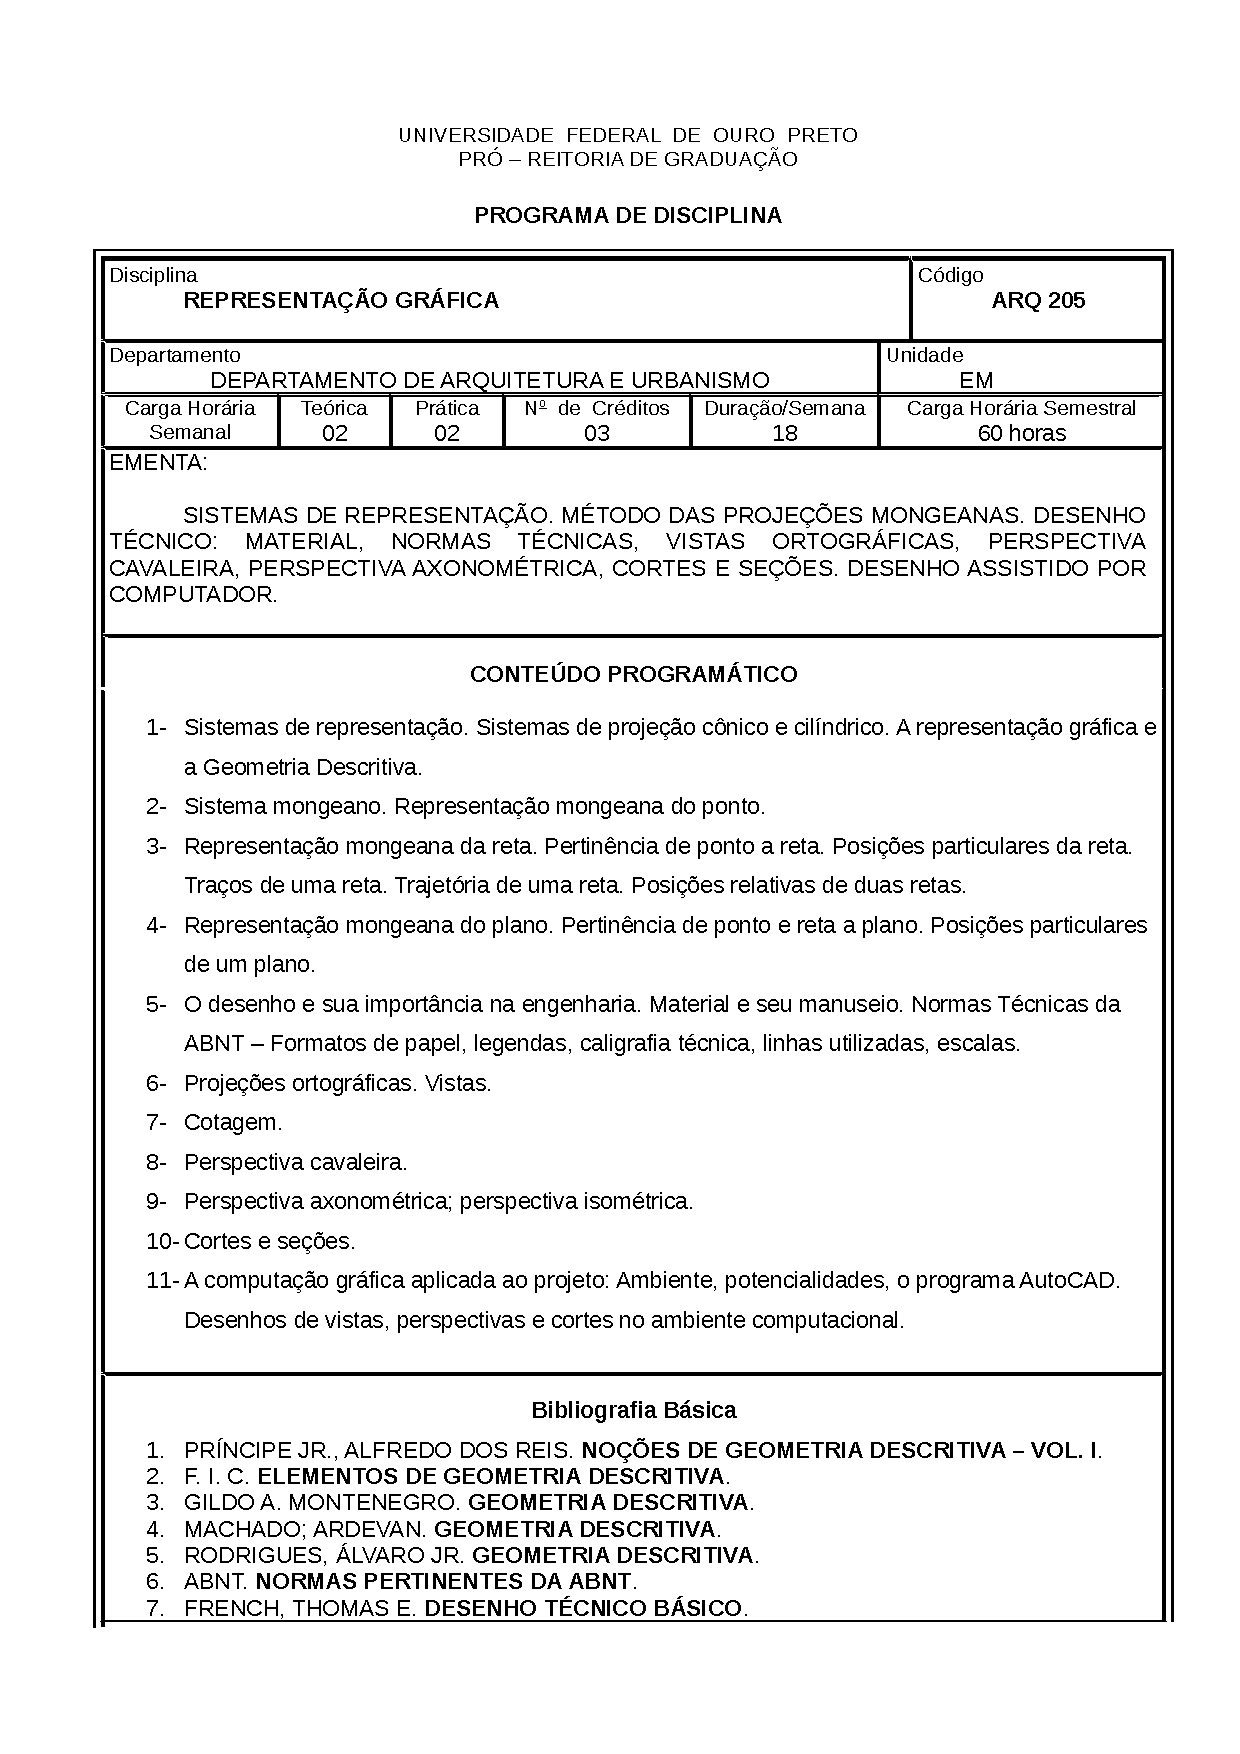
\includegraphics[scale=0.6]{capitulos/anexo1-programas-disciplina/p11.pdf}
%	\caption{Disciplina do primeiro semestre}
\end{figure}

\begin{figure}[p]
	\centering 
	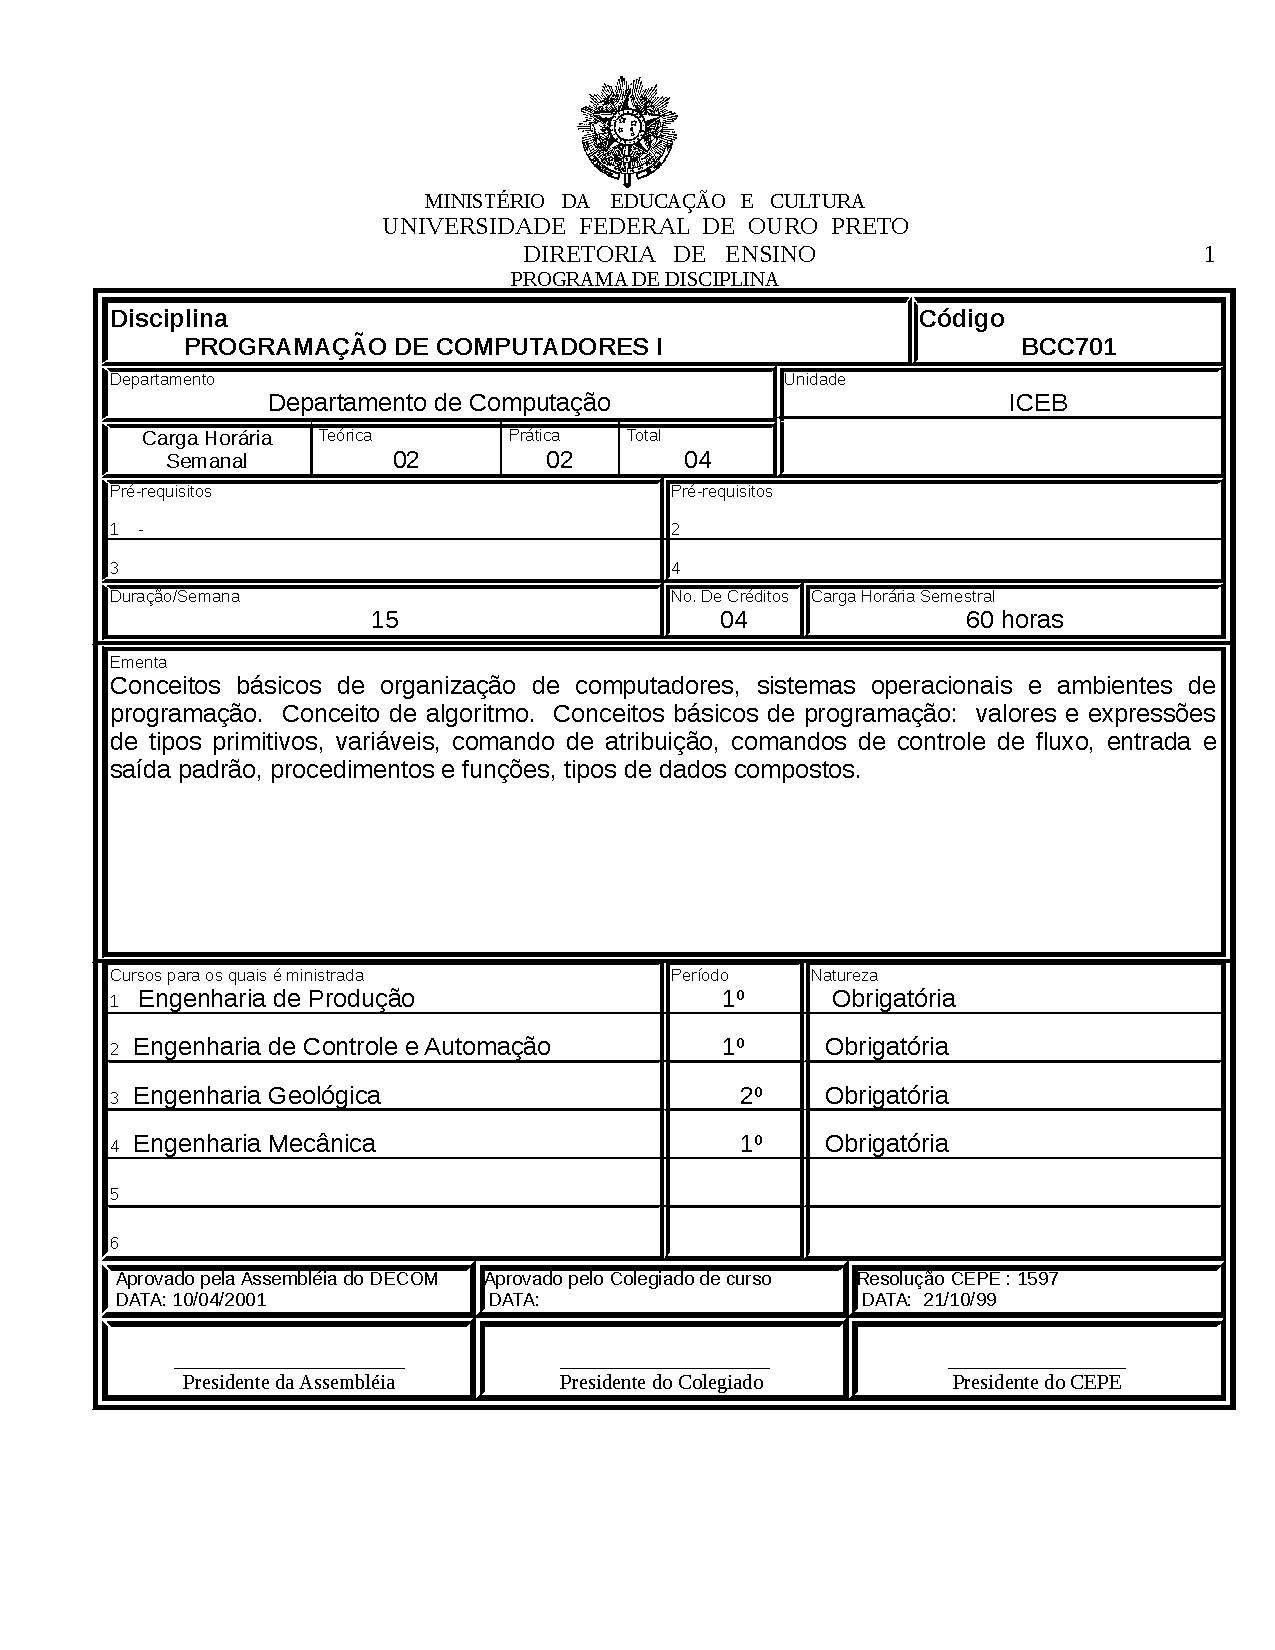
\includegraphics[scale=0.7]{capitulos/anexo1-programas-disciplina/p12.pdf}
	%	\caption{Disciplina do primeiro semestre}
\end{figure}

\begin{figure}[p]
	\centering 
	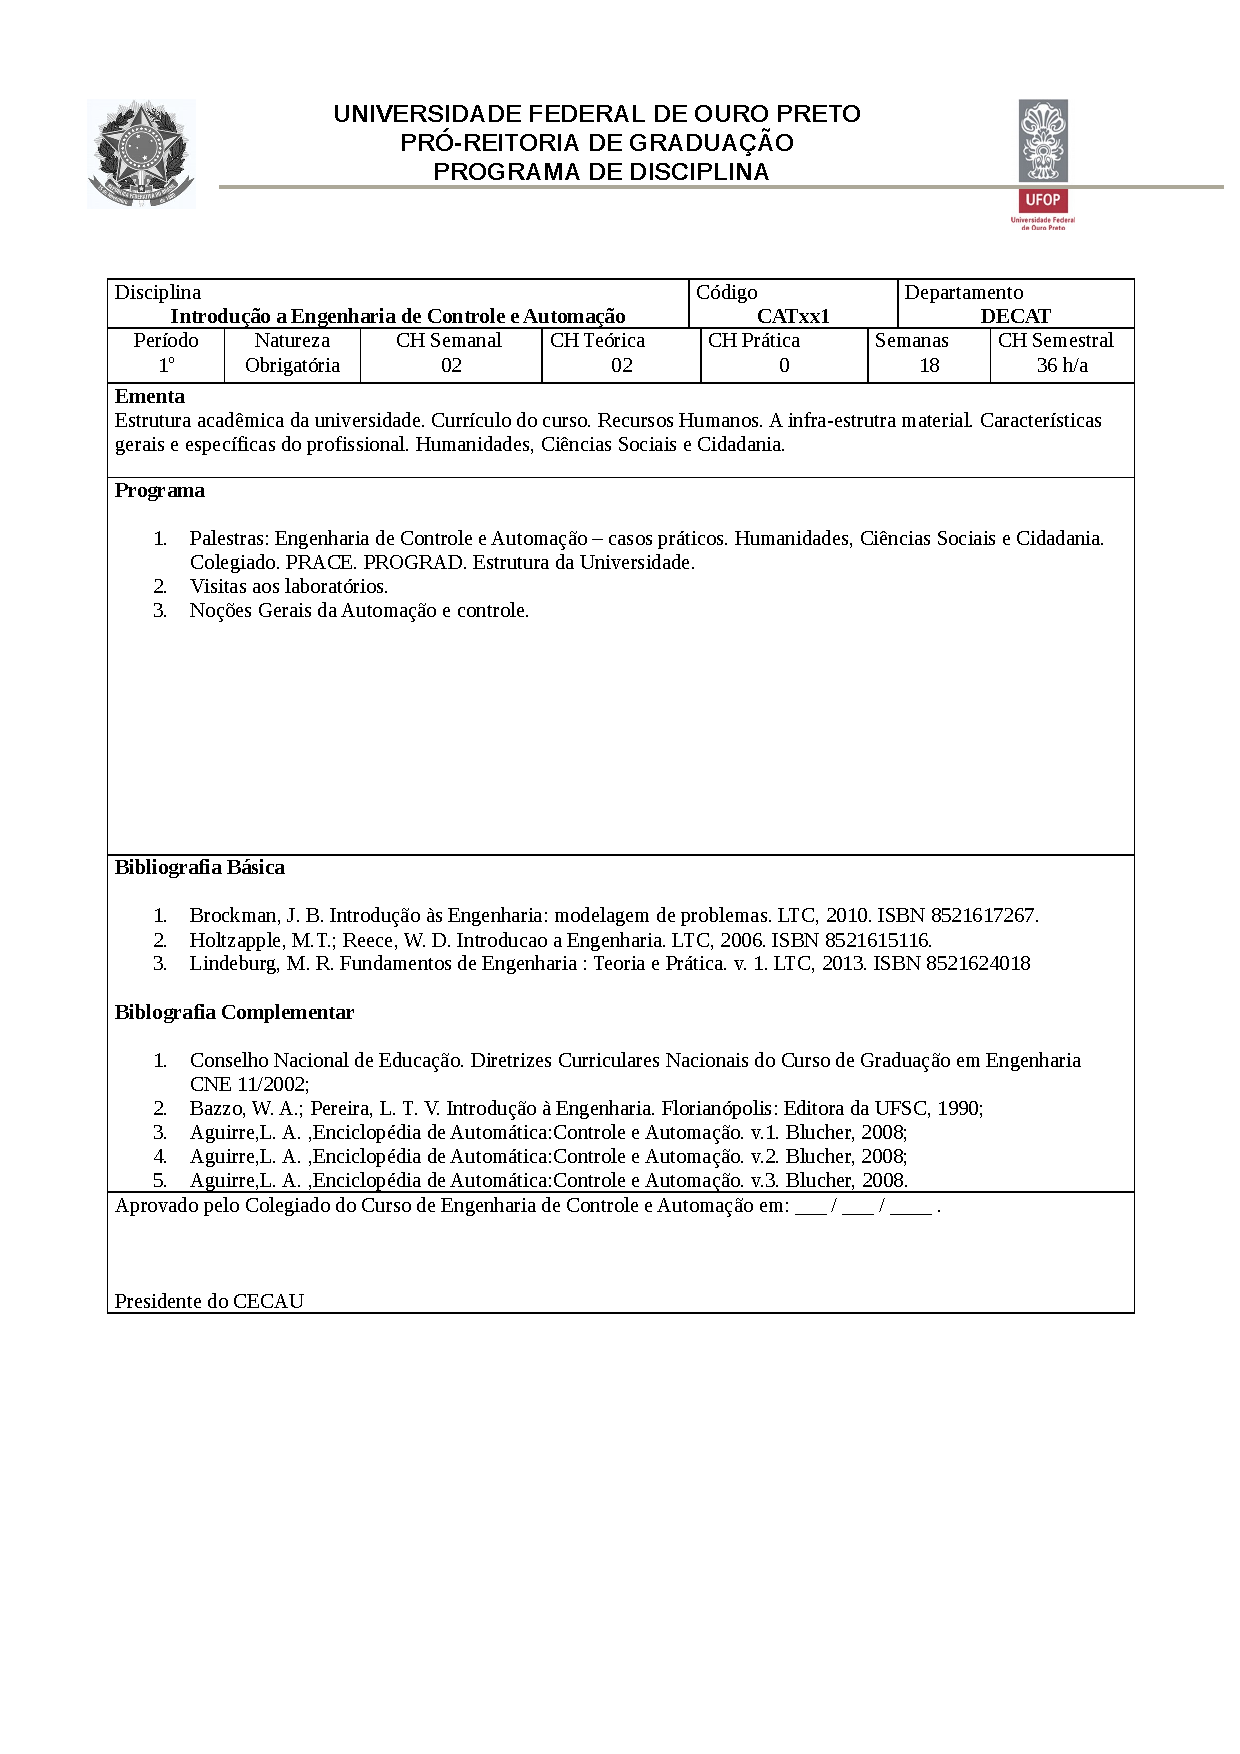
\includegraphics[scale=0.7]{capitulos/anexo1-programas-disciplina/p13.pdf}
	%	\caption{Disciplina do primeiro semestre}
\end{figure}

\begin{figure}[p]
	\centering 
	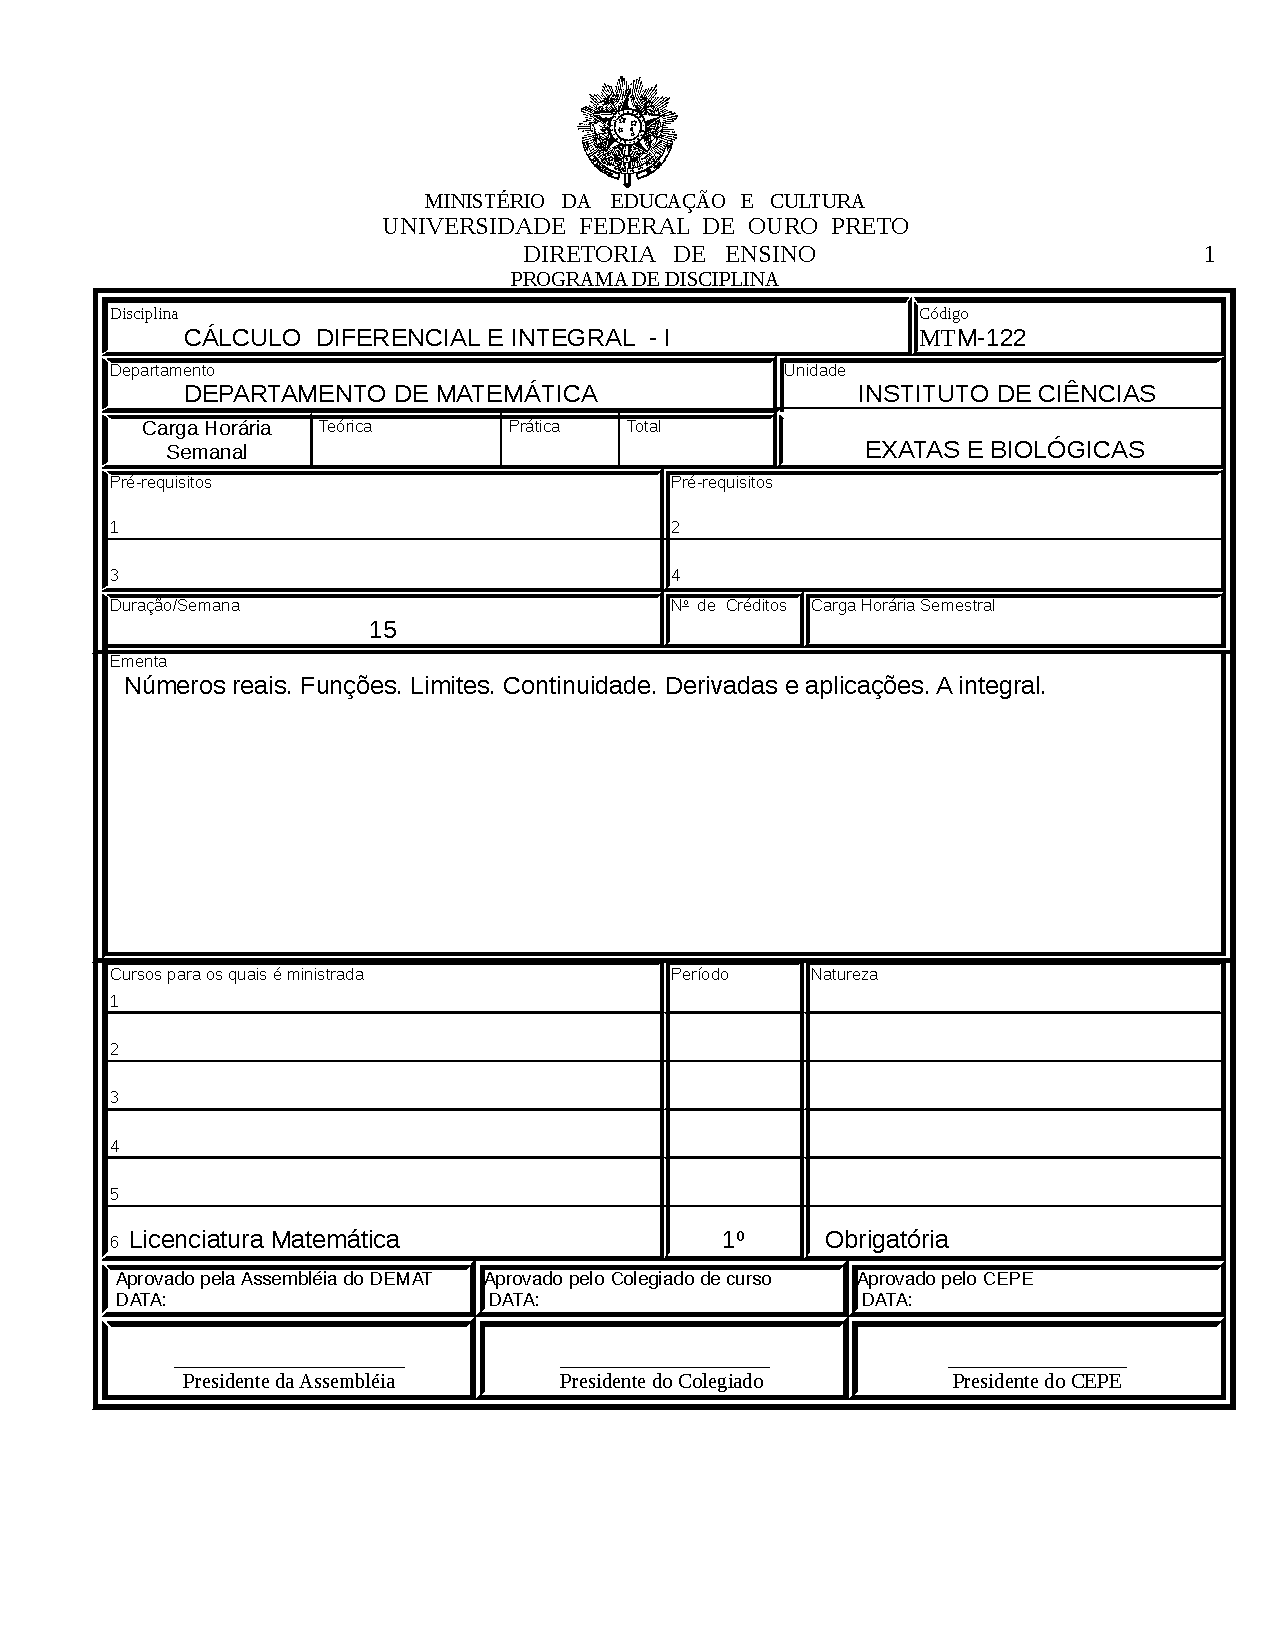
\includegraphics[scale=0.7]{capitulos/anexo1-programas-disciplina/p14.pdf}
	%	\caption{Disciplina do primeiro semestre}
\end{figure}

\begin{figure}[p]
	\centering 
	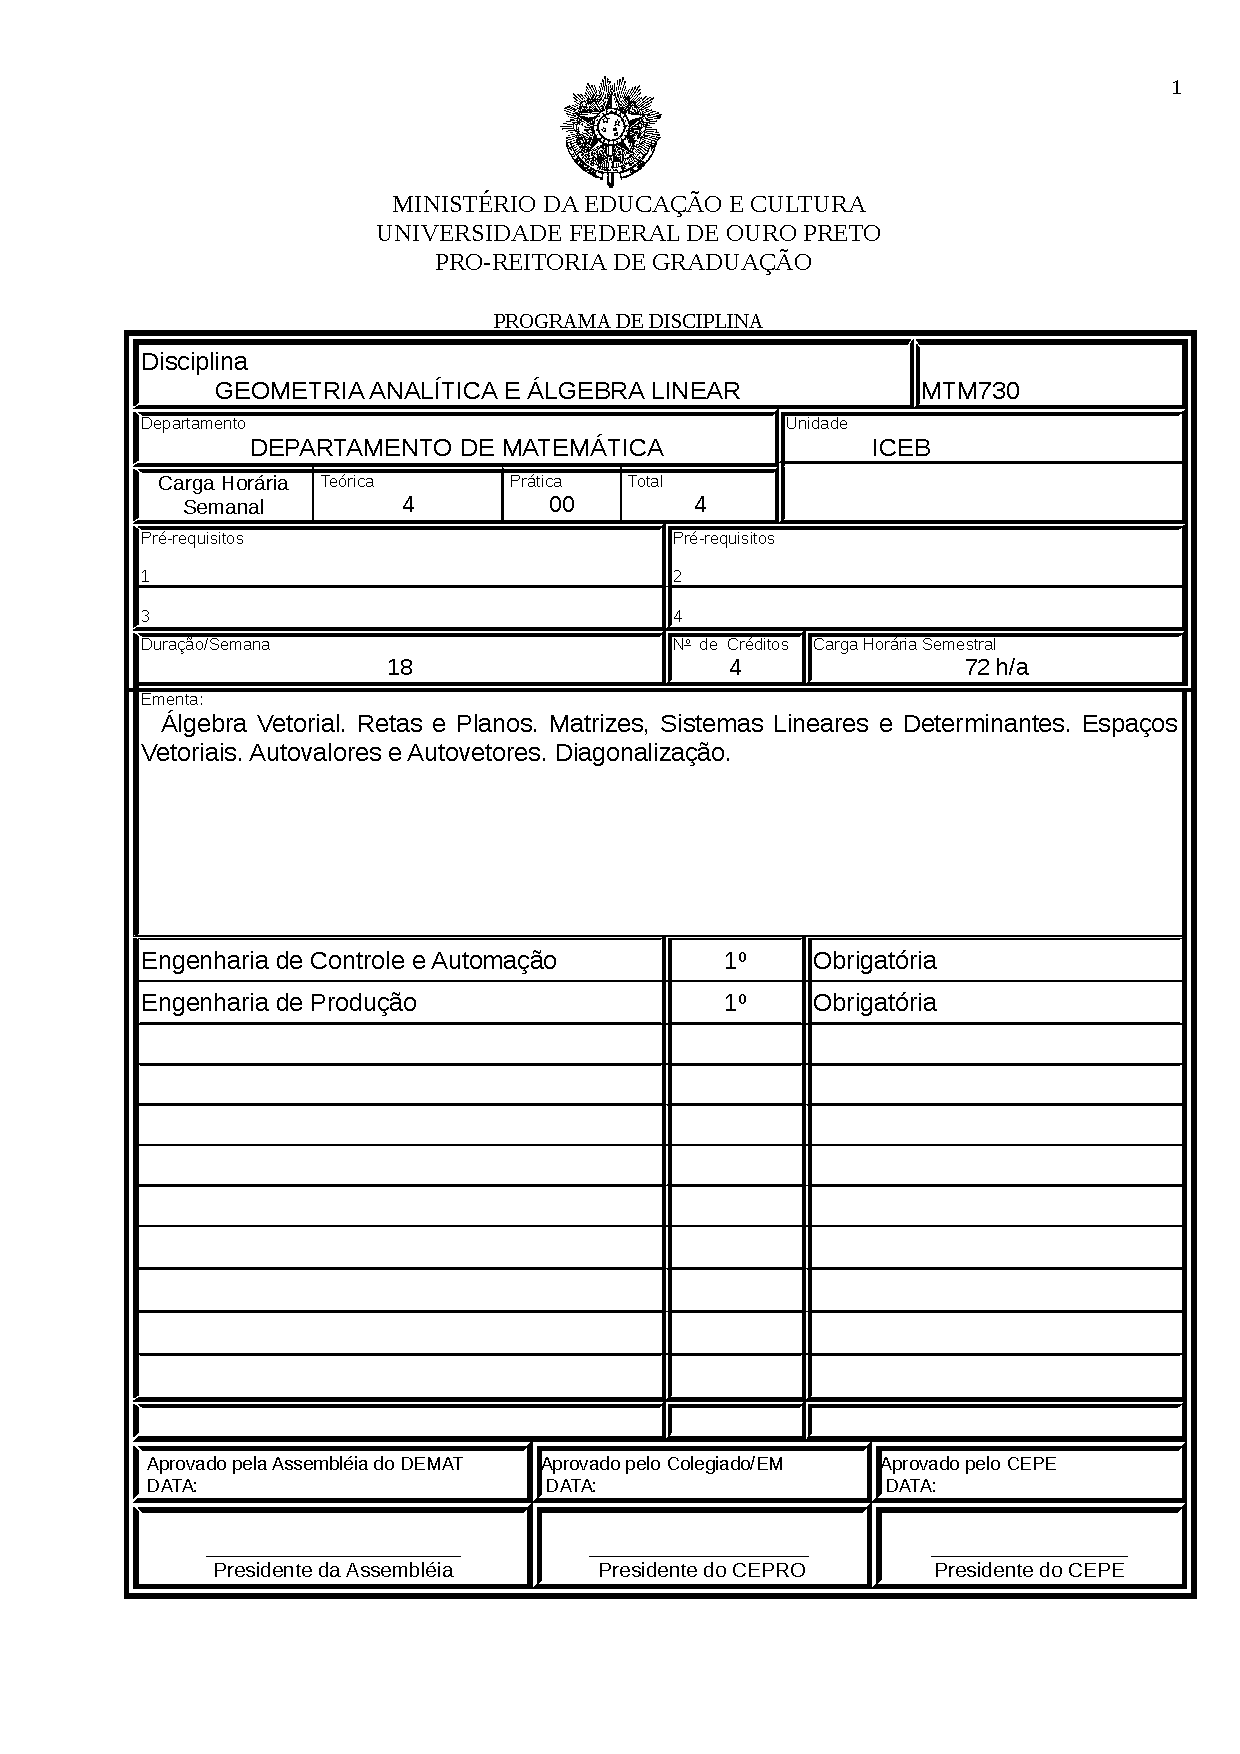
\includegraphics[scale=0.7]{capitulos/anexo1-programas-disciplina/p15.pdf}
	%	\caption{Disciplina do primeiro semestre}
\end{figure}

\begin{figure}[p]
	\centering 
	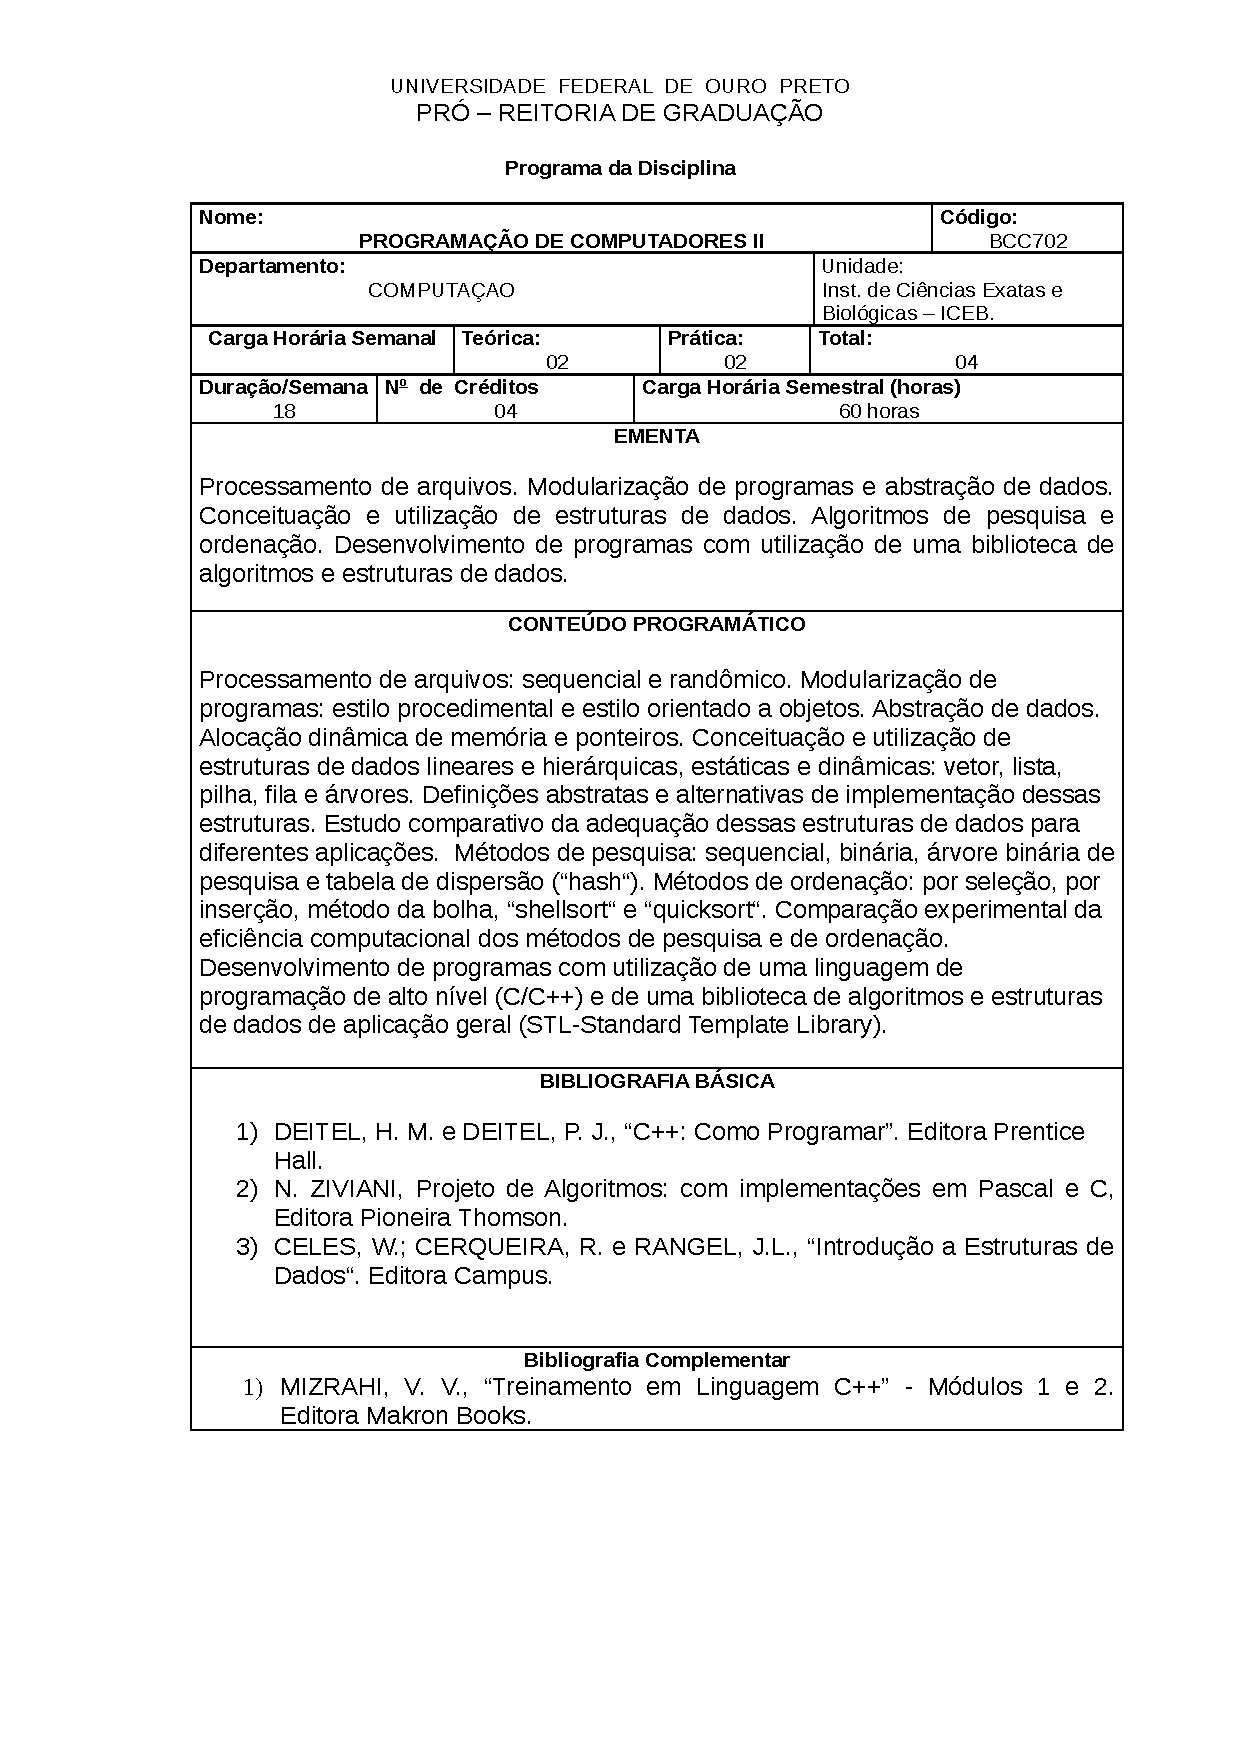
\includegraphics[scale=0.7]{capitulos/anexo1-programas-disciplina/p21.pdf}
	%	\caption{Disciplina do primeiro semestre}
\end{figure}

\begin{figure}[p]
	\centering 
	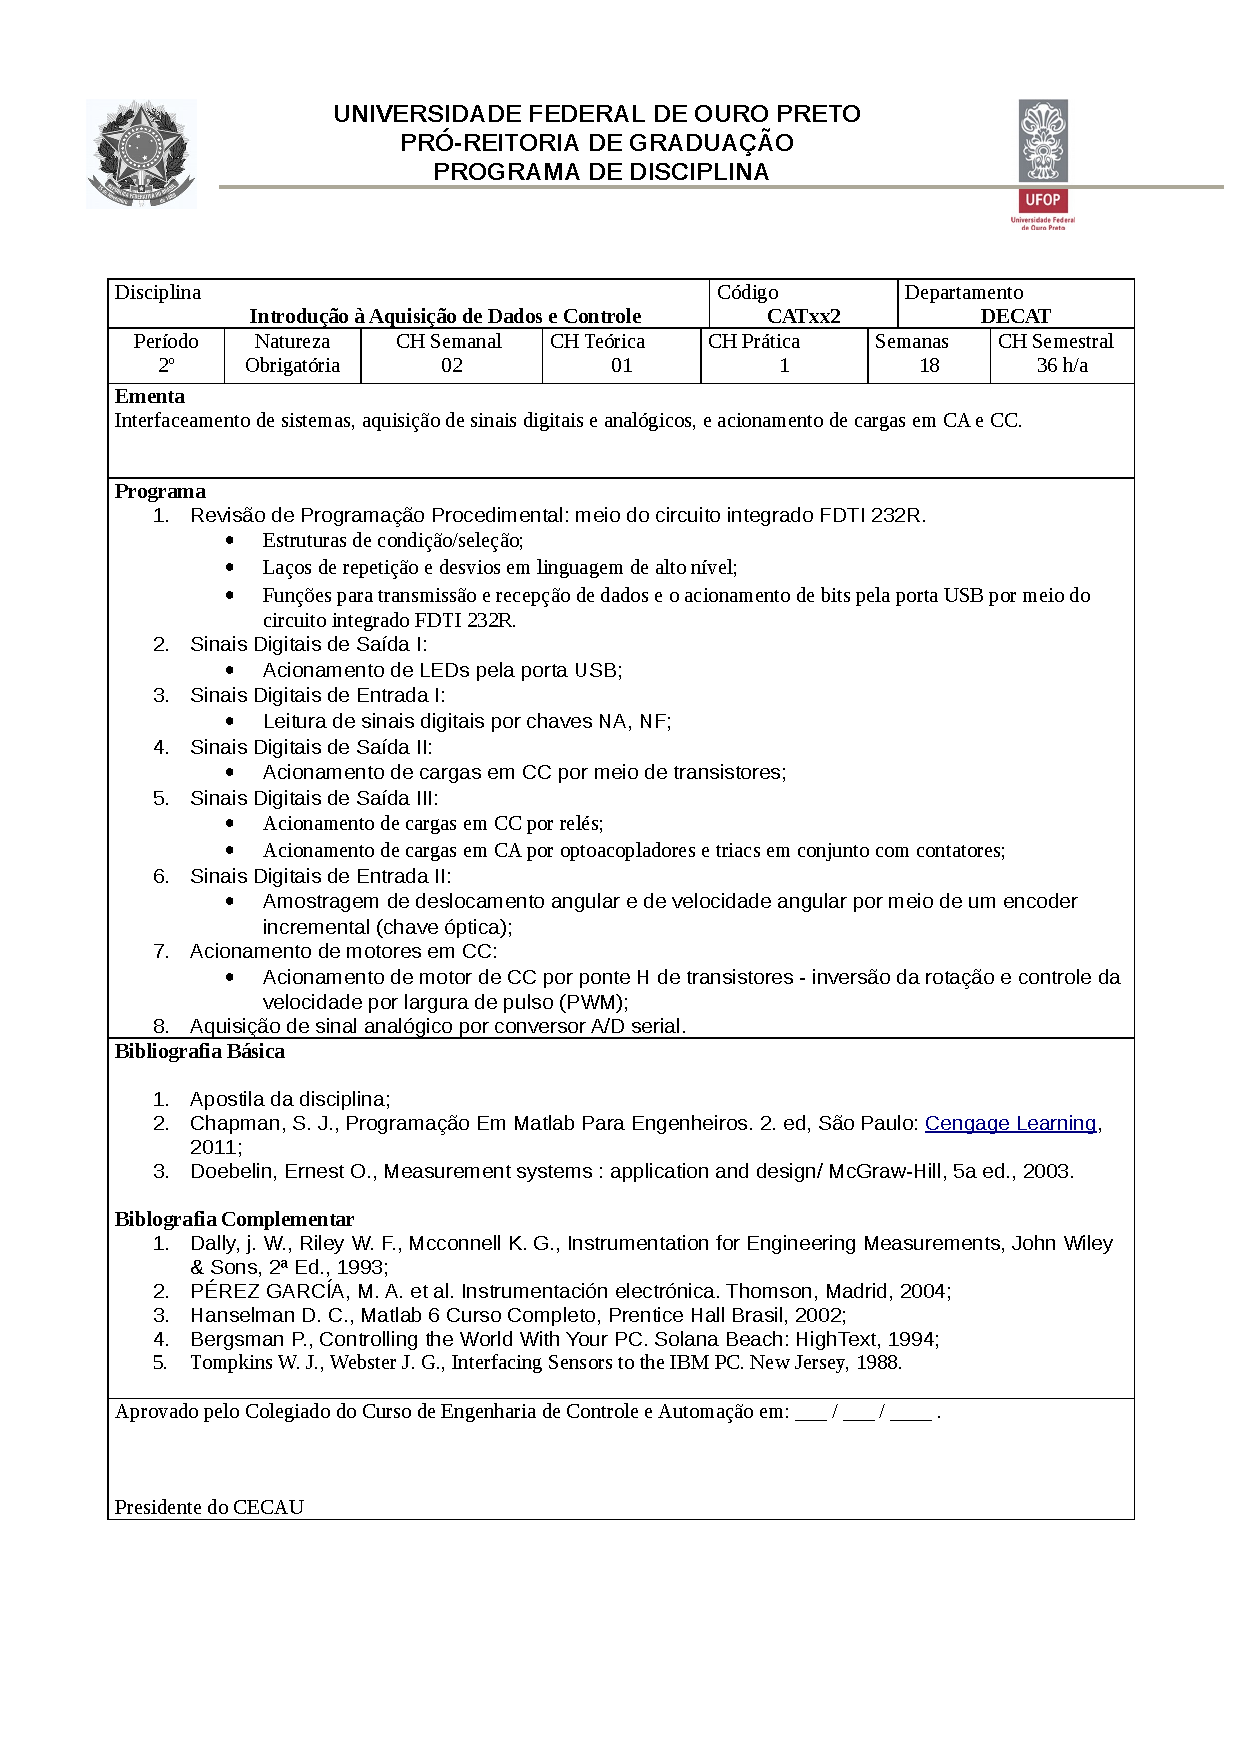
\includegraphics[scale=0.7]{capitulos/anexo1-programas-disciplina/p22.pdf}
	%	\caption{Disciplina do primeiro semestre}
\end{figure}

\begin{figure}[p]
	\centering 
	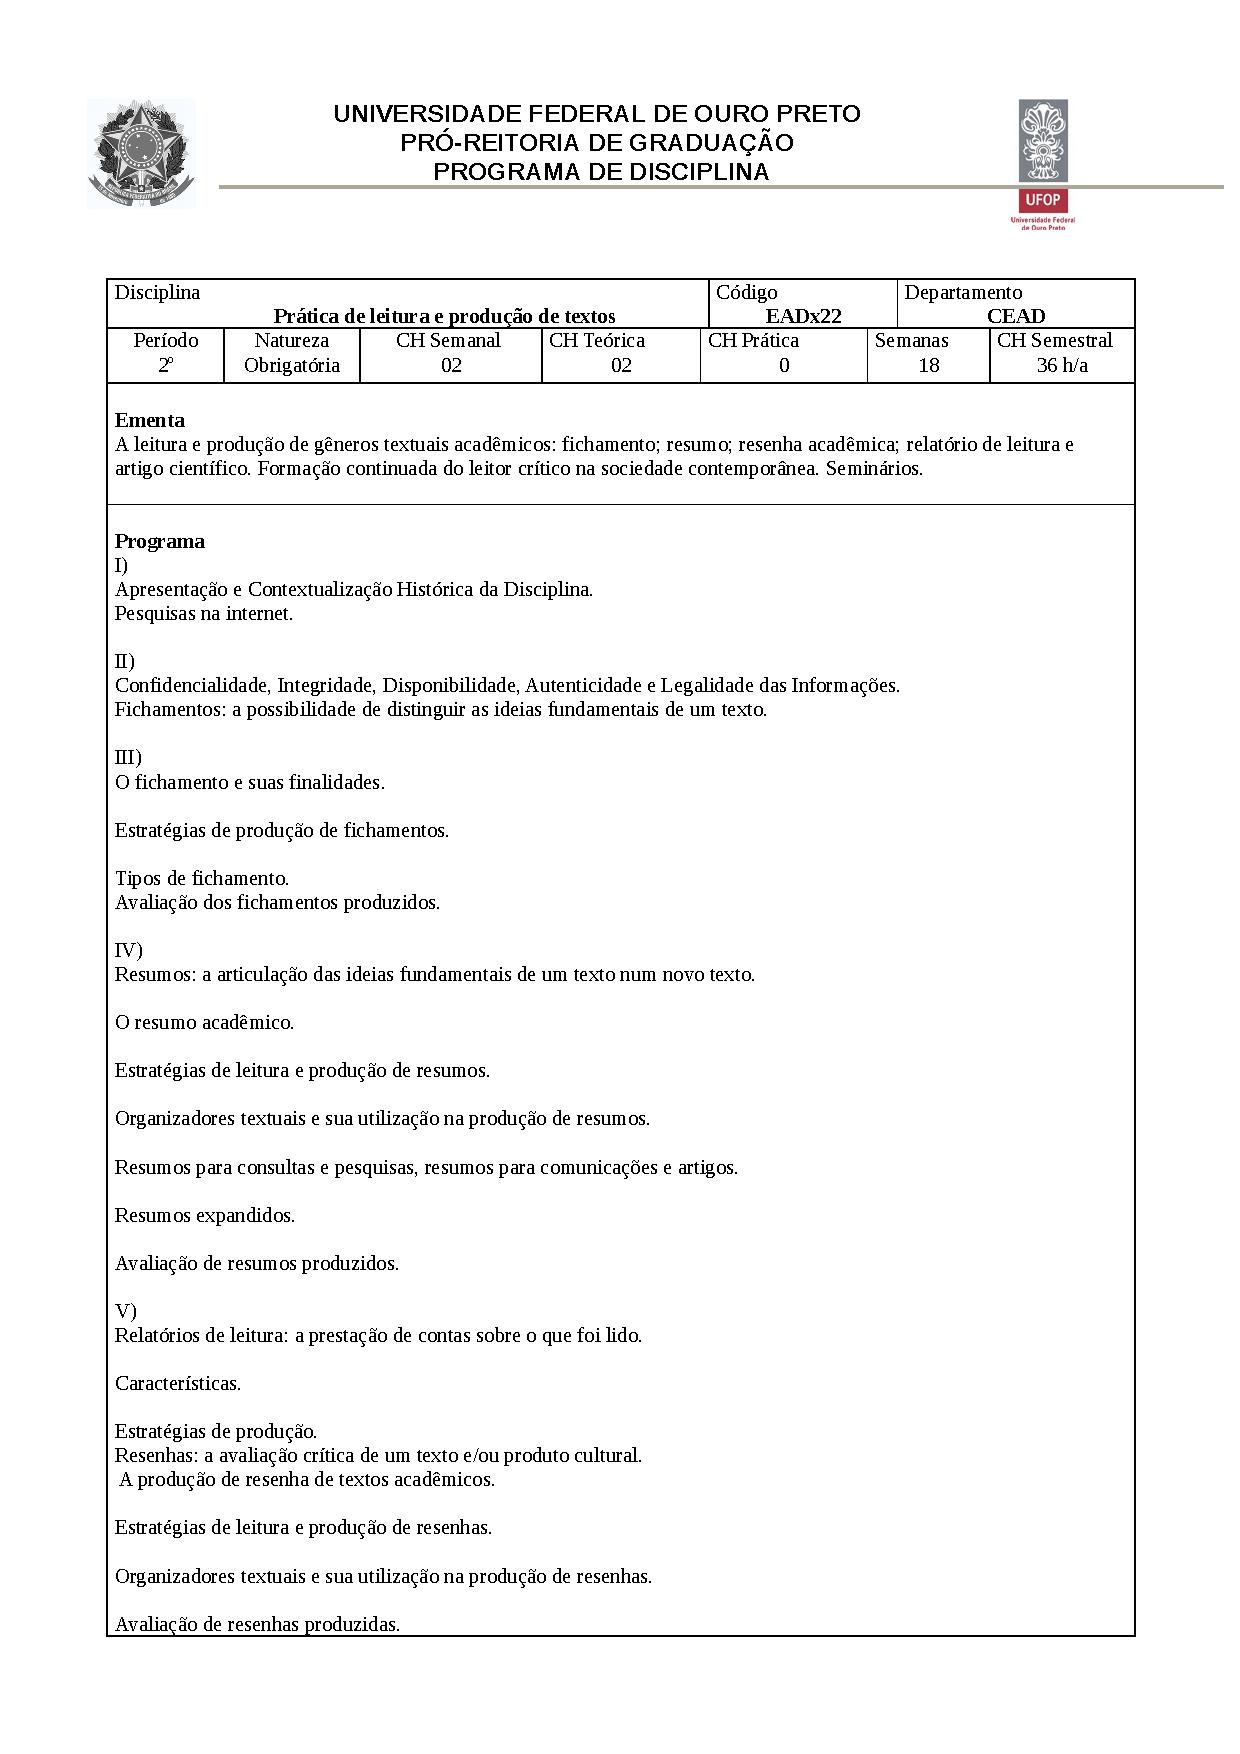
\includegraphics[scale=0.7]{capitulos/anexo1-programas-disciplina/p23.pdf}
	%	\caption{Disciplina do primeiro semestre}
\end{figure}

\begin{figure}[p]
	\centering 
	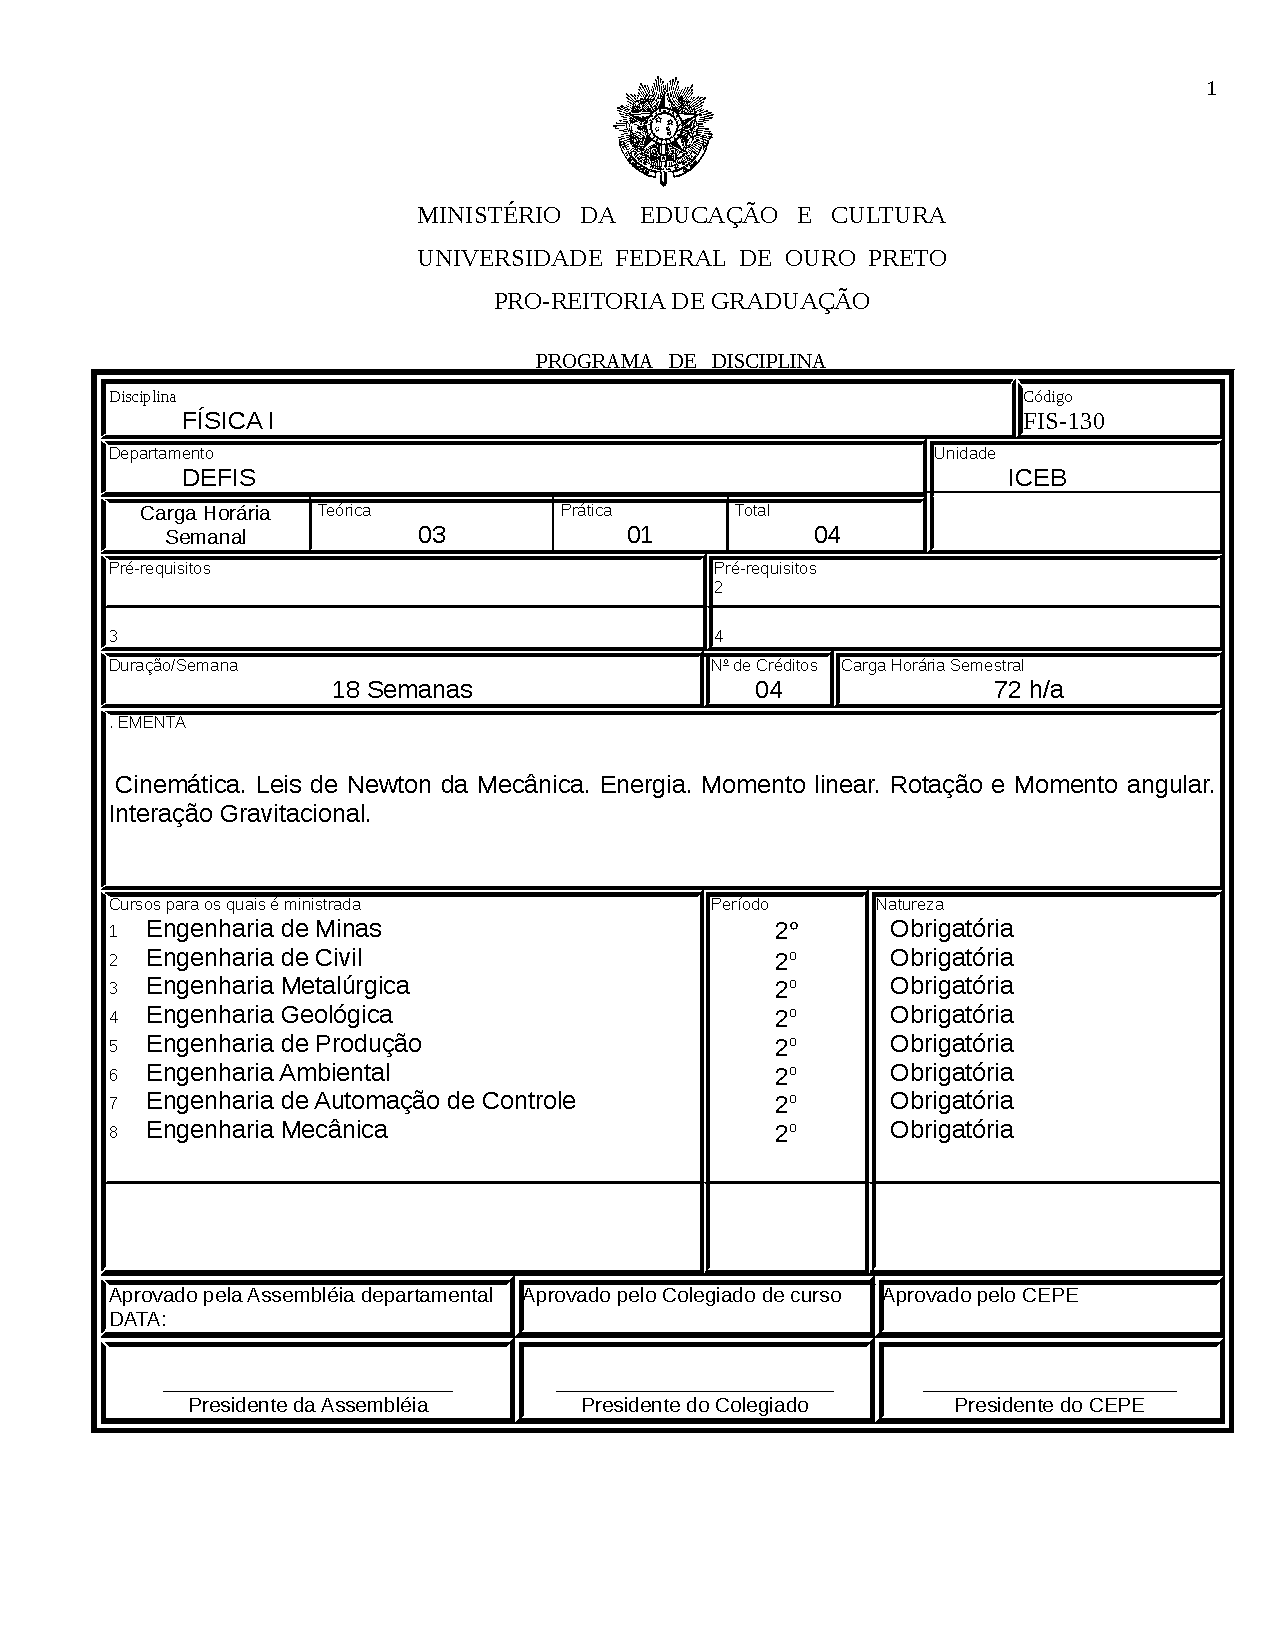
\includegraphics[scale=0.7]{capitulos/anexo1-programas-disciplina/p24.pdf}
	%	\caption{Disciplina do primeiro semestre}
\end{figure}

\begin{figure}[p]
	\centering 
	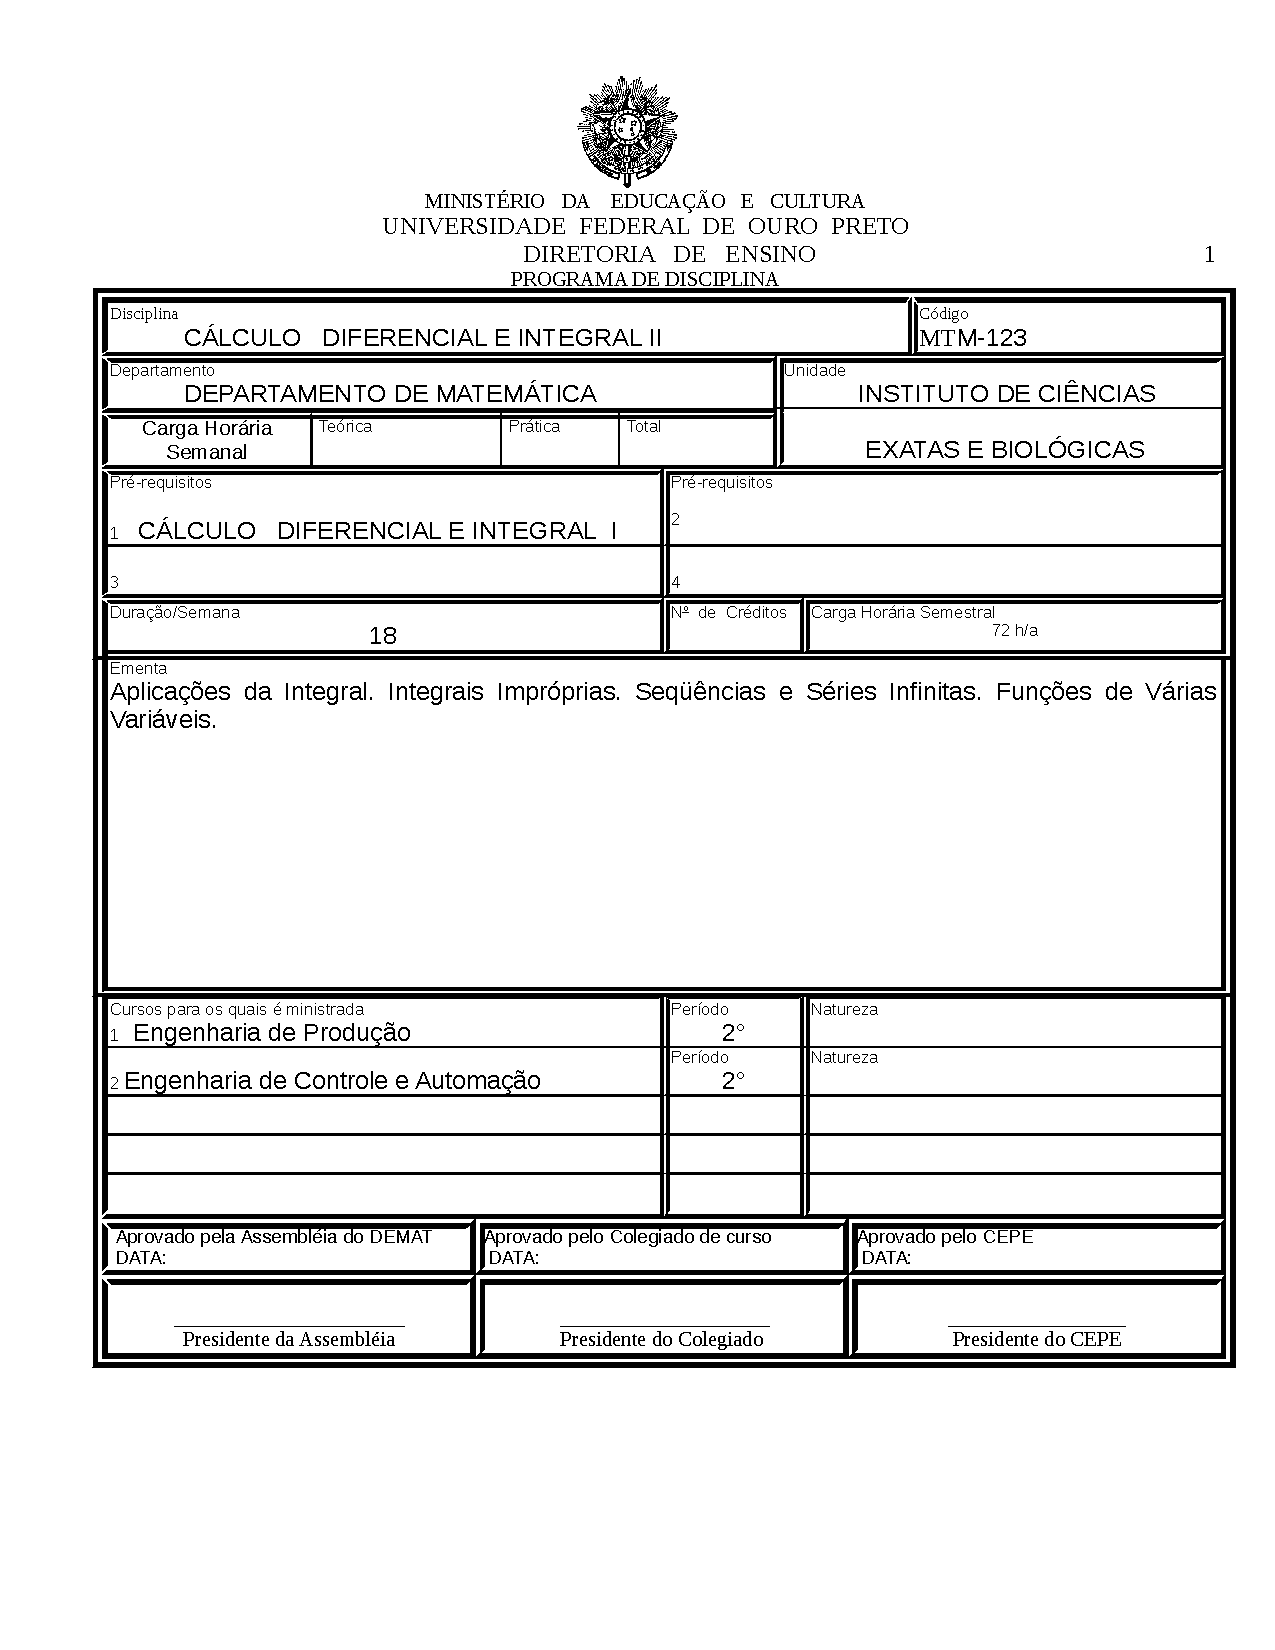
\includegraphics[scale=0.7]{capitulos/anexo1-programas-disciplina/p25.pdf}
	%	\caption{Disciplina do primeiro semestre}
\end{figure}

\begin{figure}[p]
	\centering 
	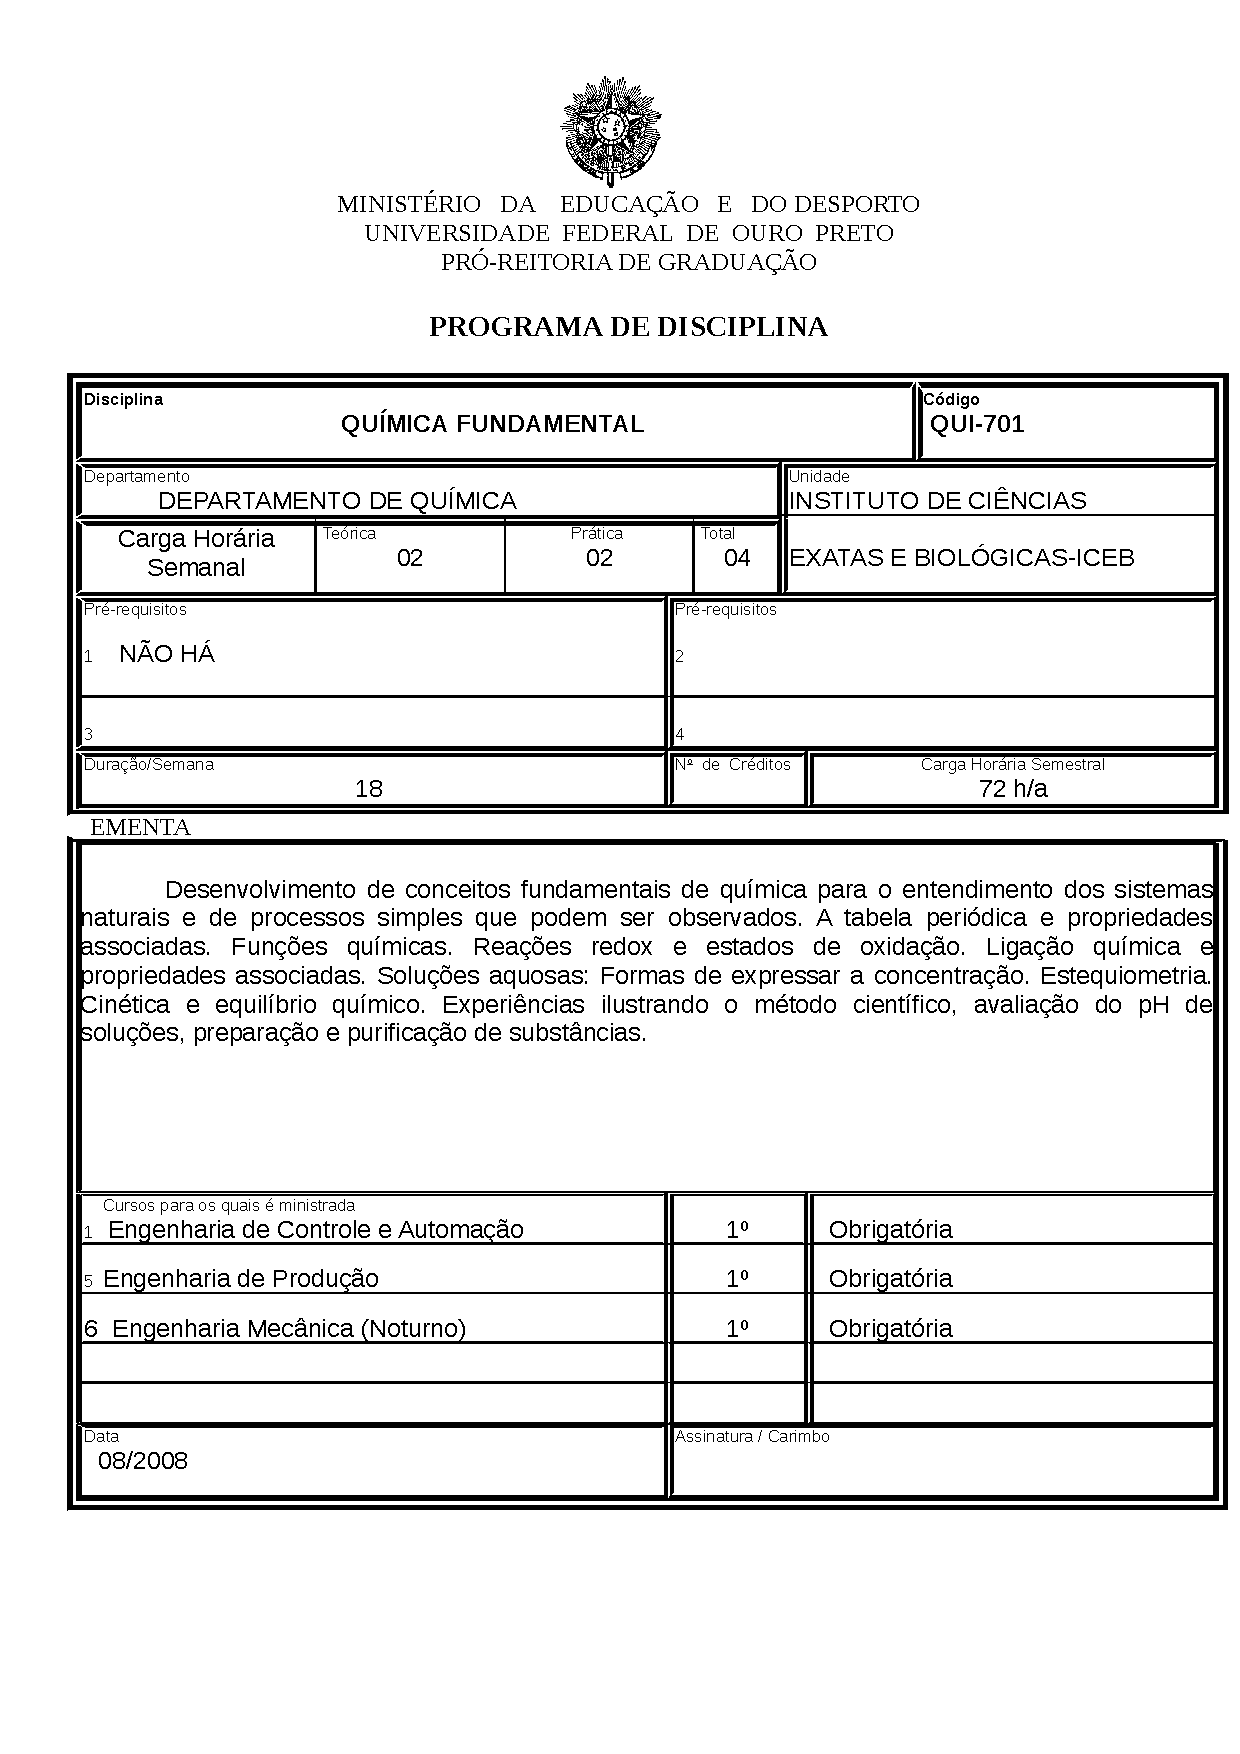
\includegraphics[scale=0.7]{capitulos/anexo1-programas-disciplina/p26.pdf}
	%	\caption{Disciplina do primeiro semestre}
\end{figure}

% terceiro semestre
\begin{figure}[p]
	\centering 
	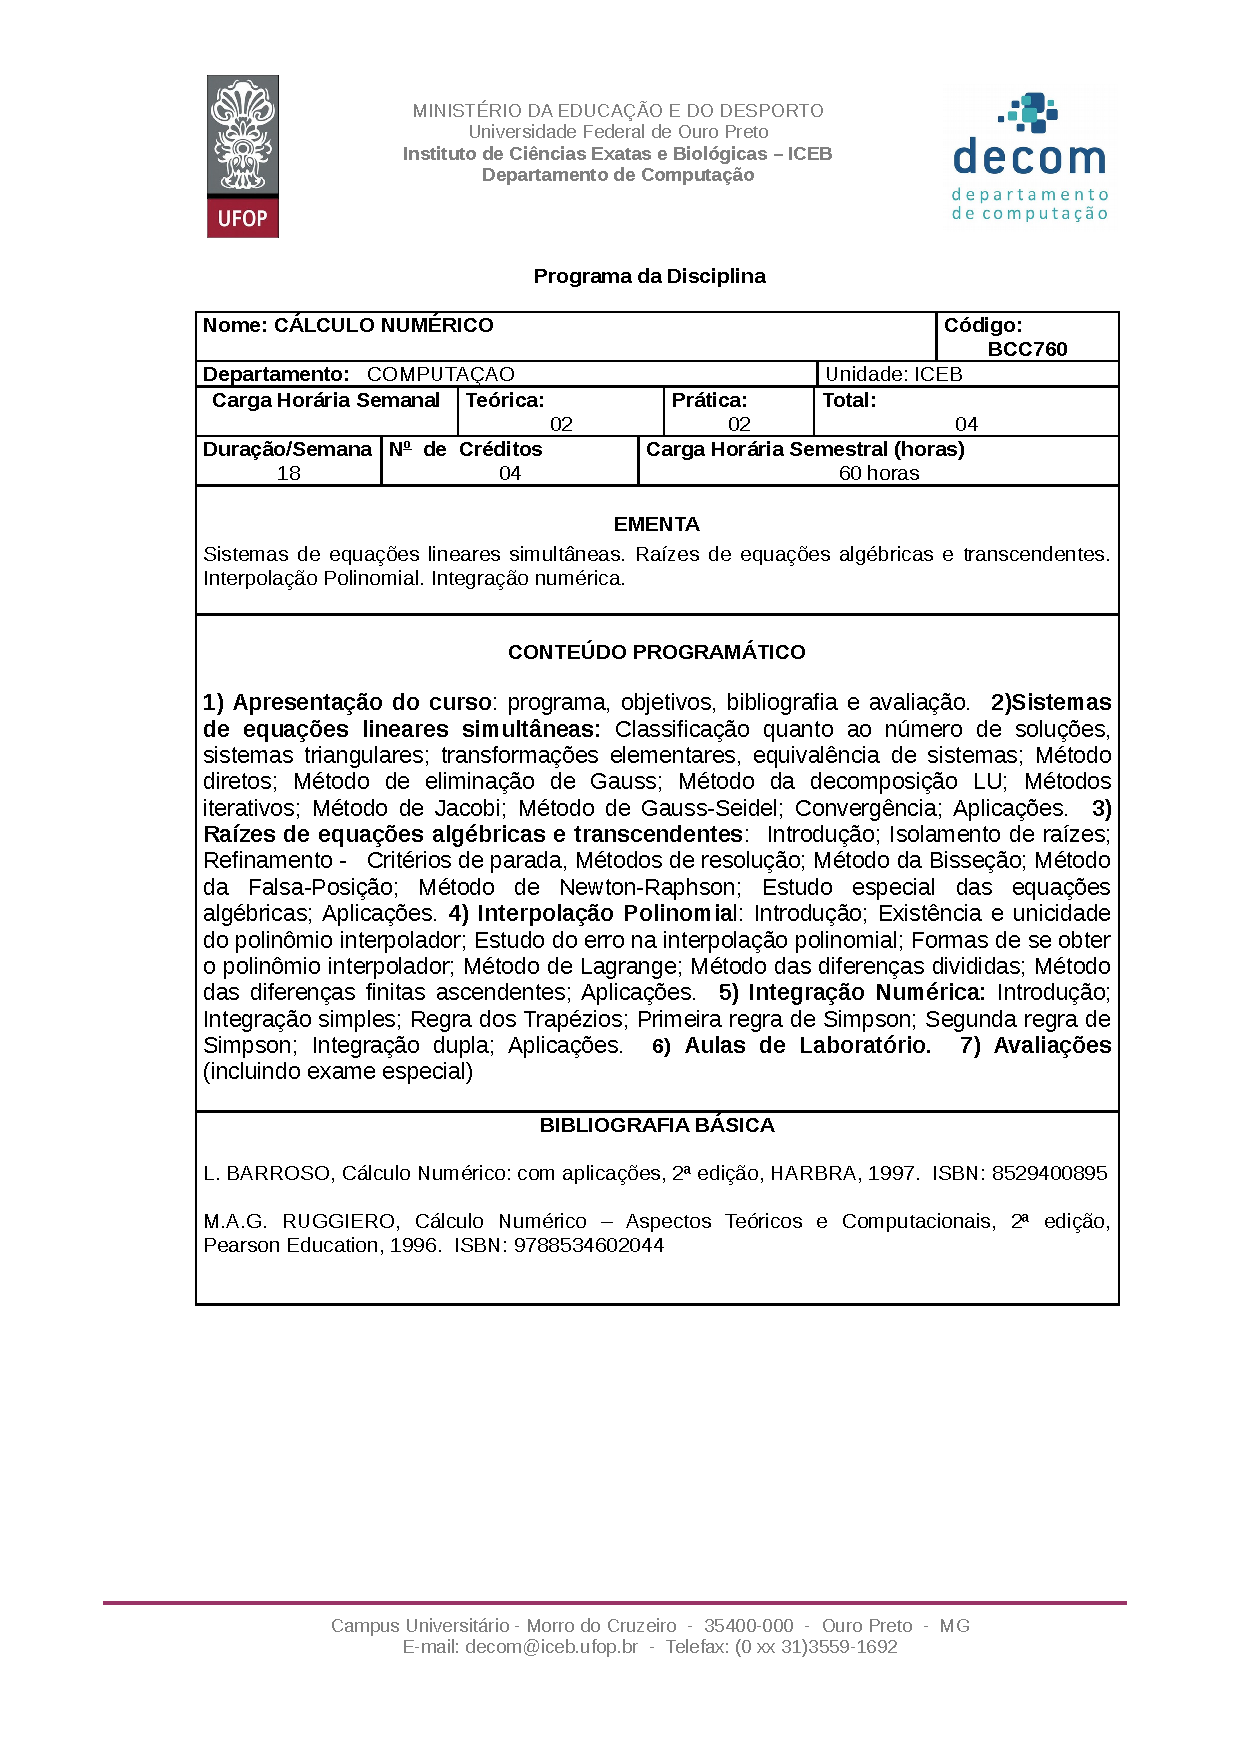
\includegraphics[scale=0.7]{capitulos/anexo1-programas-disciplina/p31.pdf}
	%	\caption{Disciplina do primeiro semestre}
\end{figure}

\begin{figure}[p]
	\centering 
	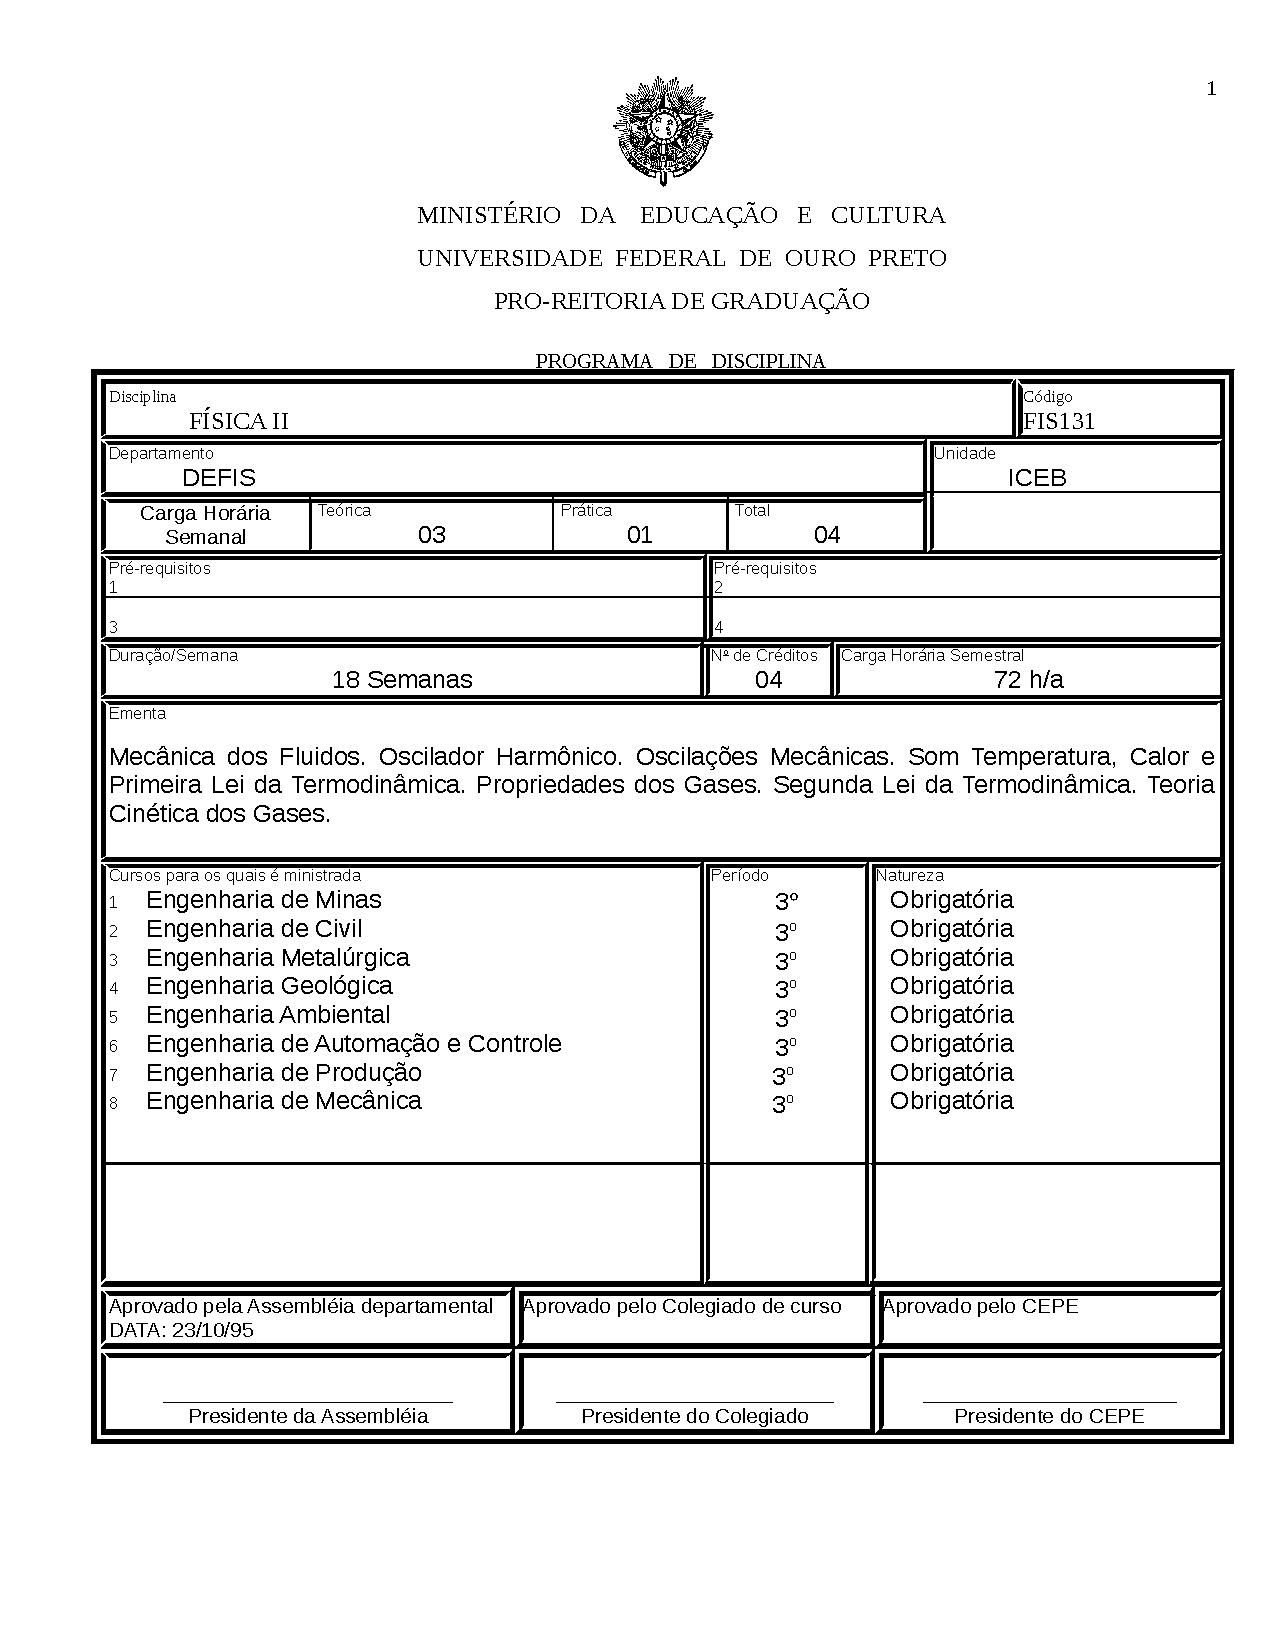
\includegraphics[scale=0.7]{capitulos/anexo1-programas-disciplina/p32.pdf}
	%	\caption{Disciplina do primeiro semestre}
\end{figure}

\begin{figure}[p]
	\centering 
	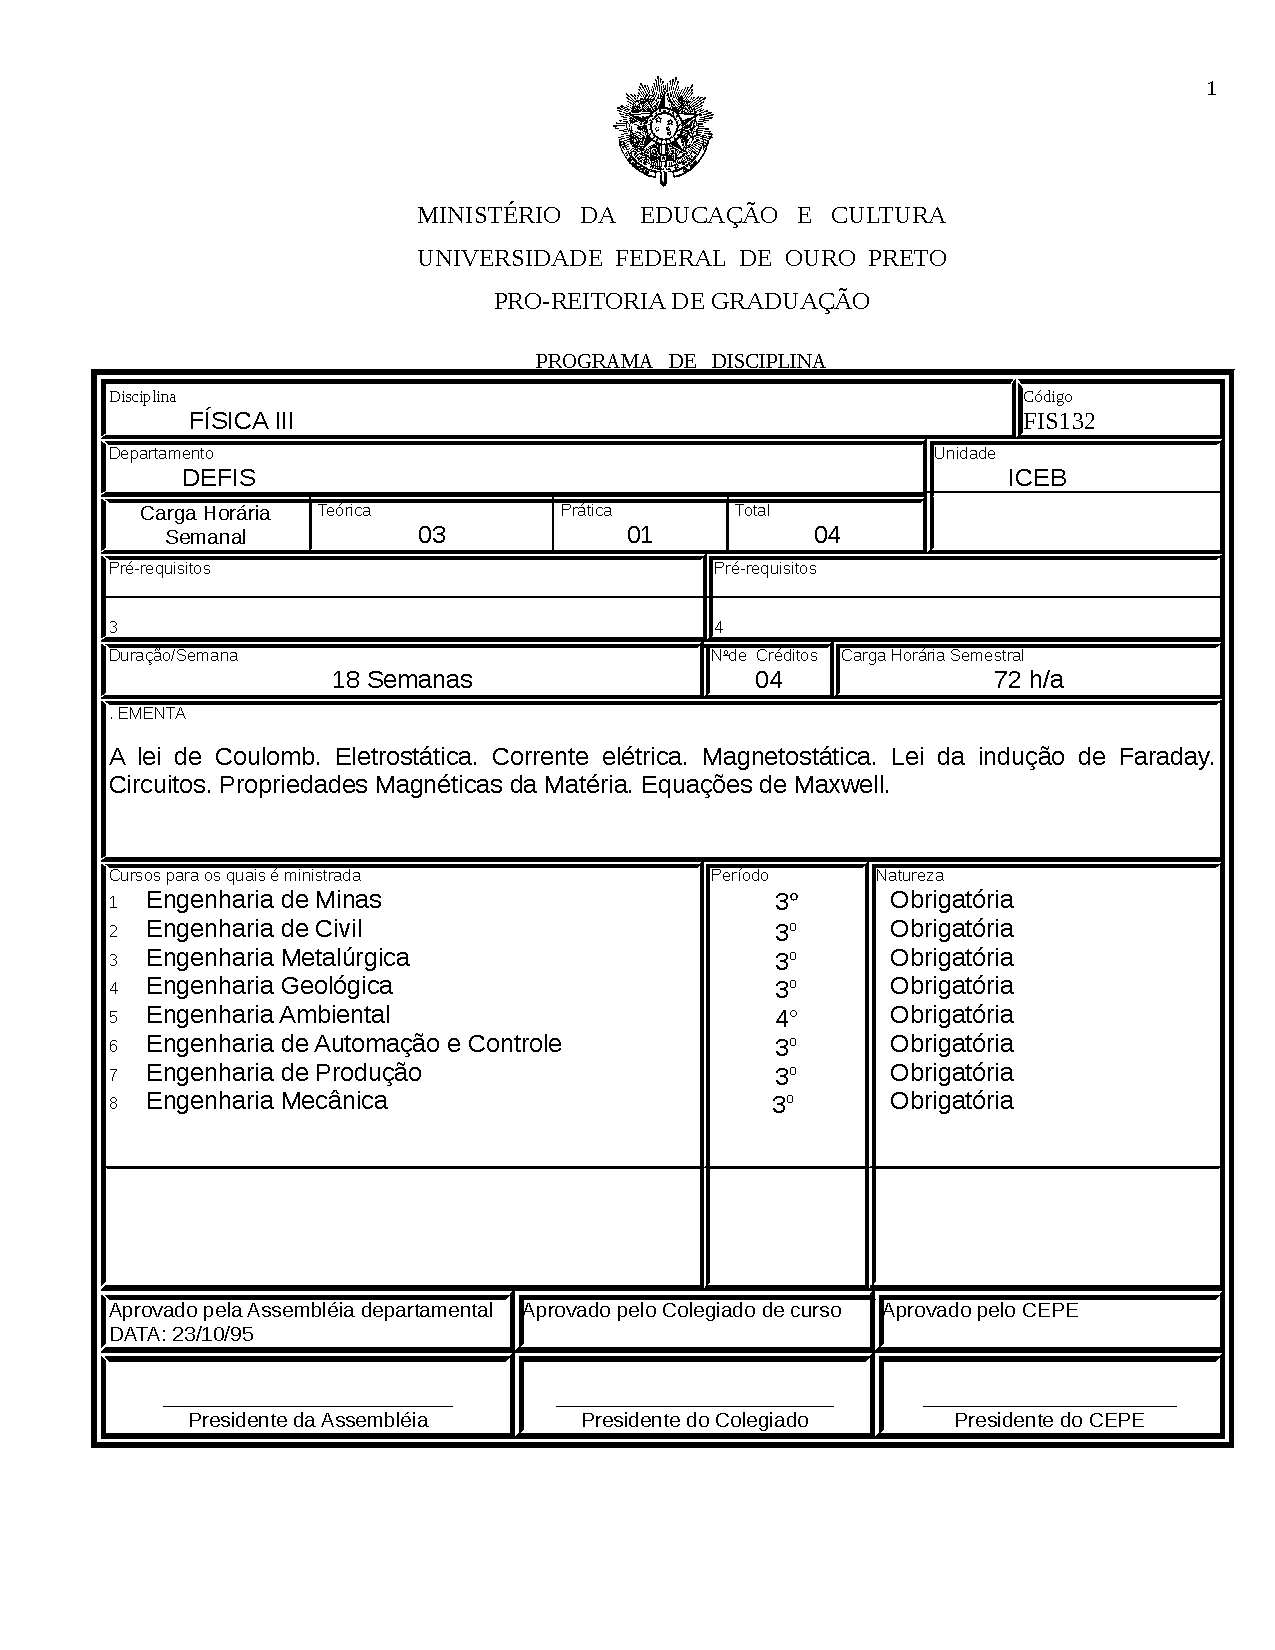
\includegraphics[scale=0.7]{capitulos/anexo1-programas-disciplina/p33.pdf}
	%	\caption{Disciplina do primeiro semestre}
\end{figure}

\begin{figure}[p]
	\centering 
	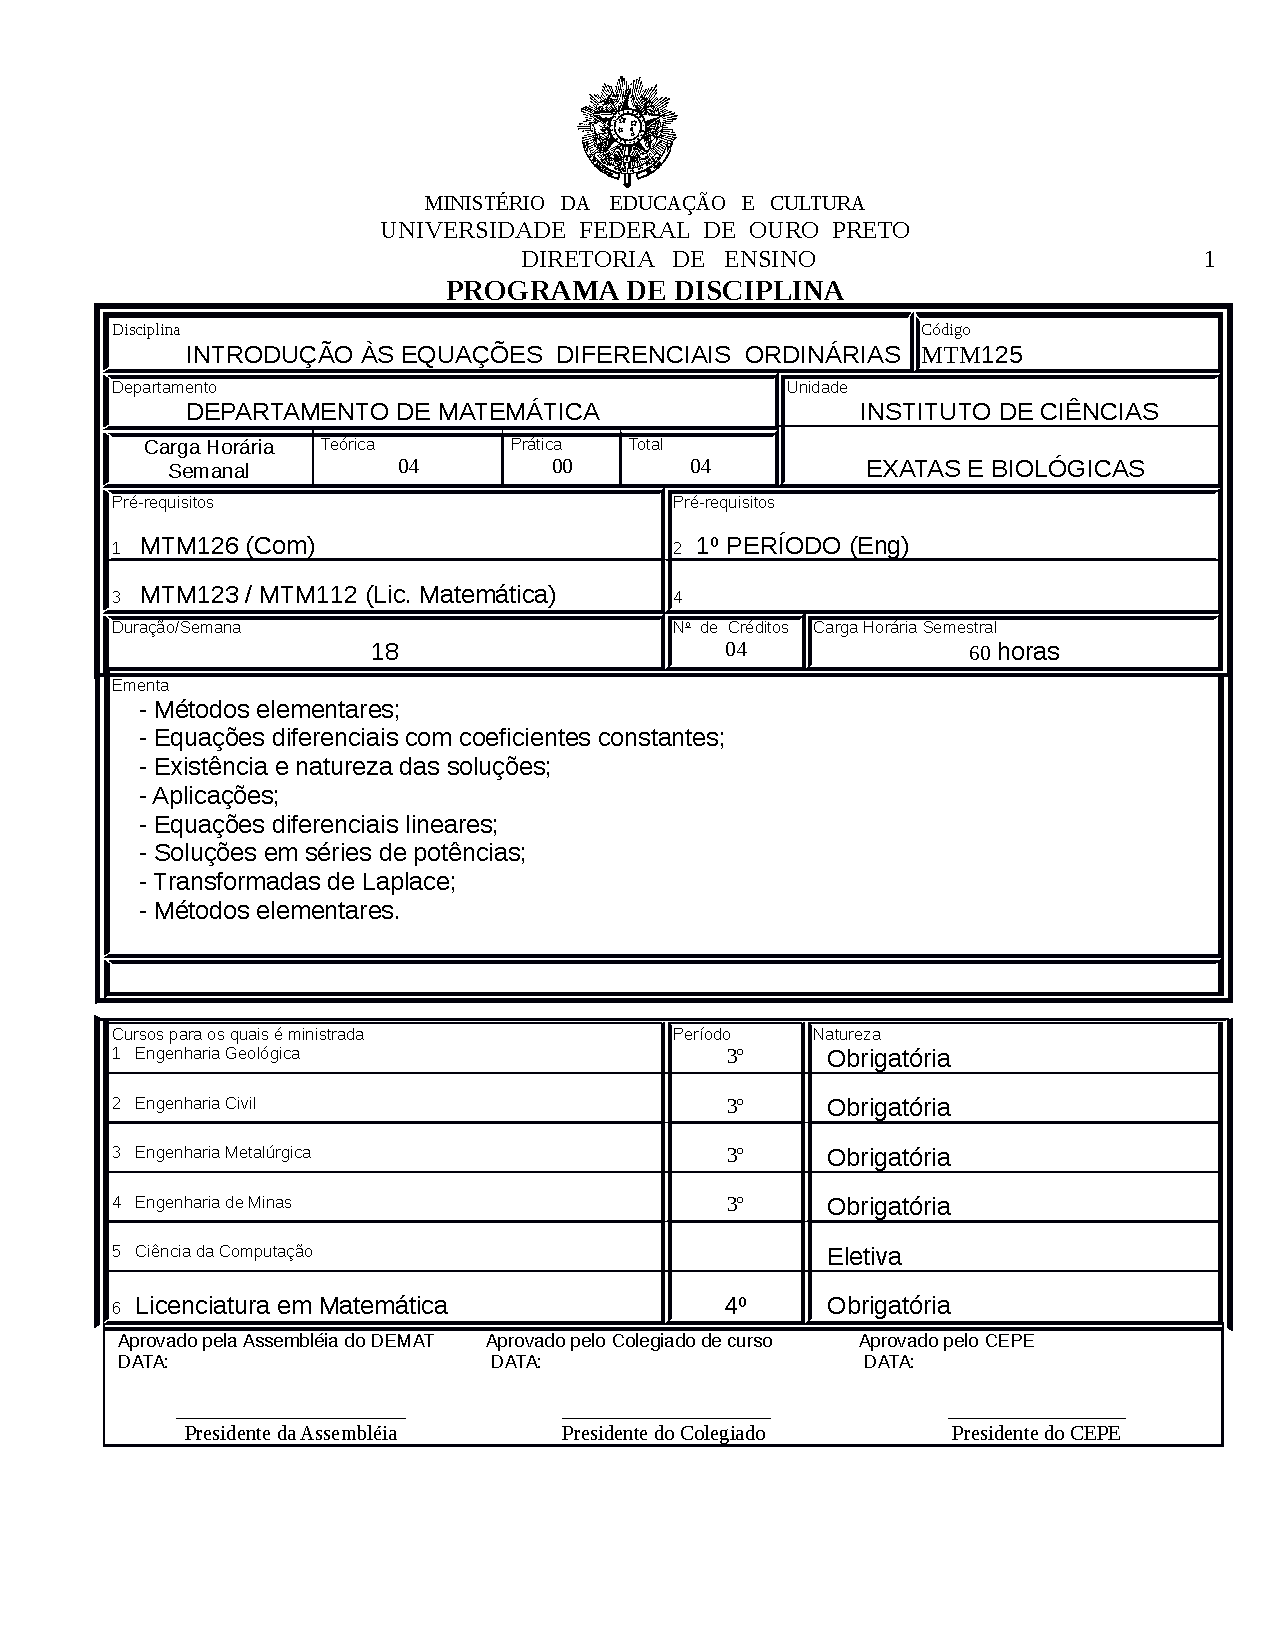
\includegraphics[scale=0.7]{capitulos/anexo1-programas-disciplina/p34.pdf}
	%	\caption{Disciplina do primeiro semestre}
\end{figure}

\begin{figure}[p]
	\centering 
	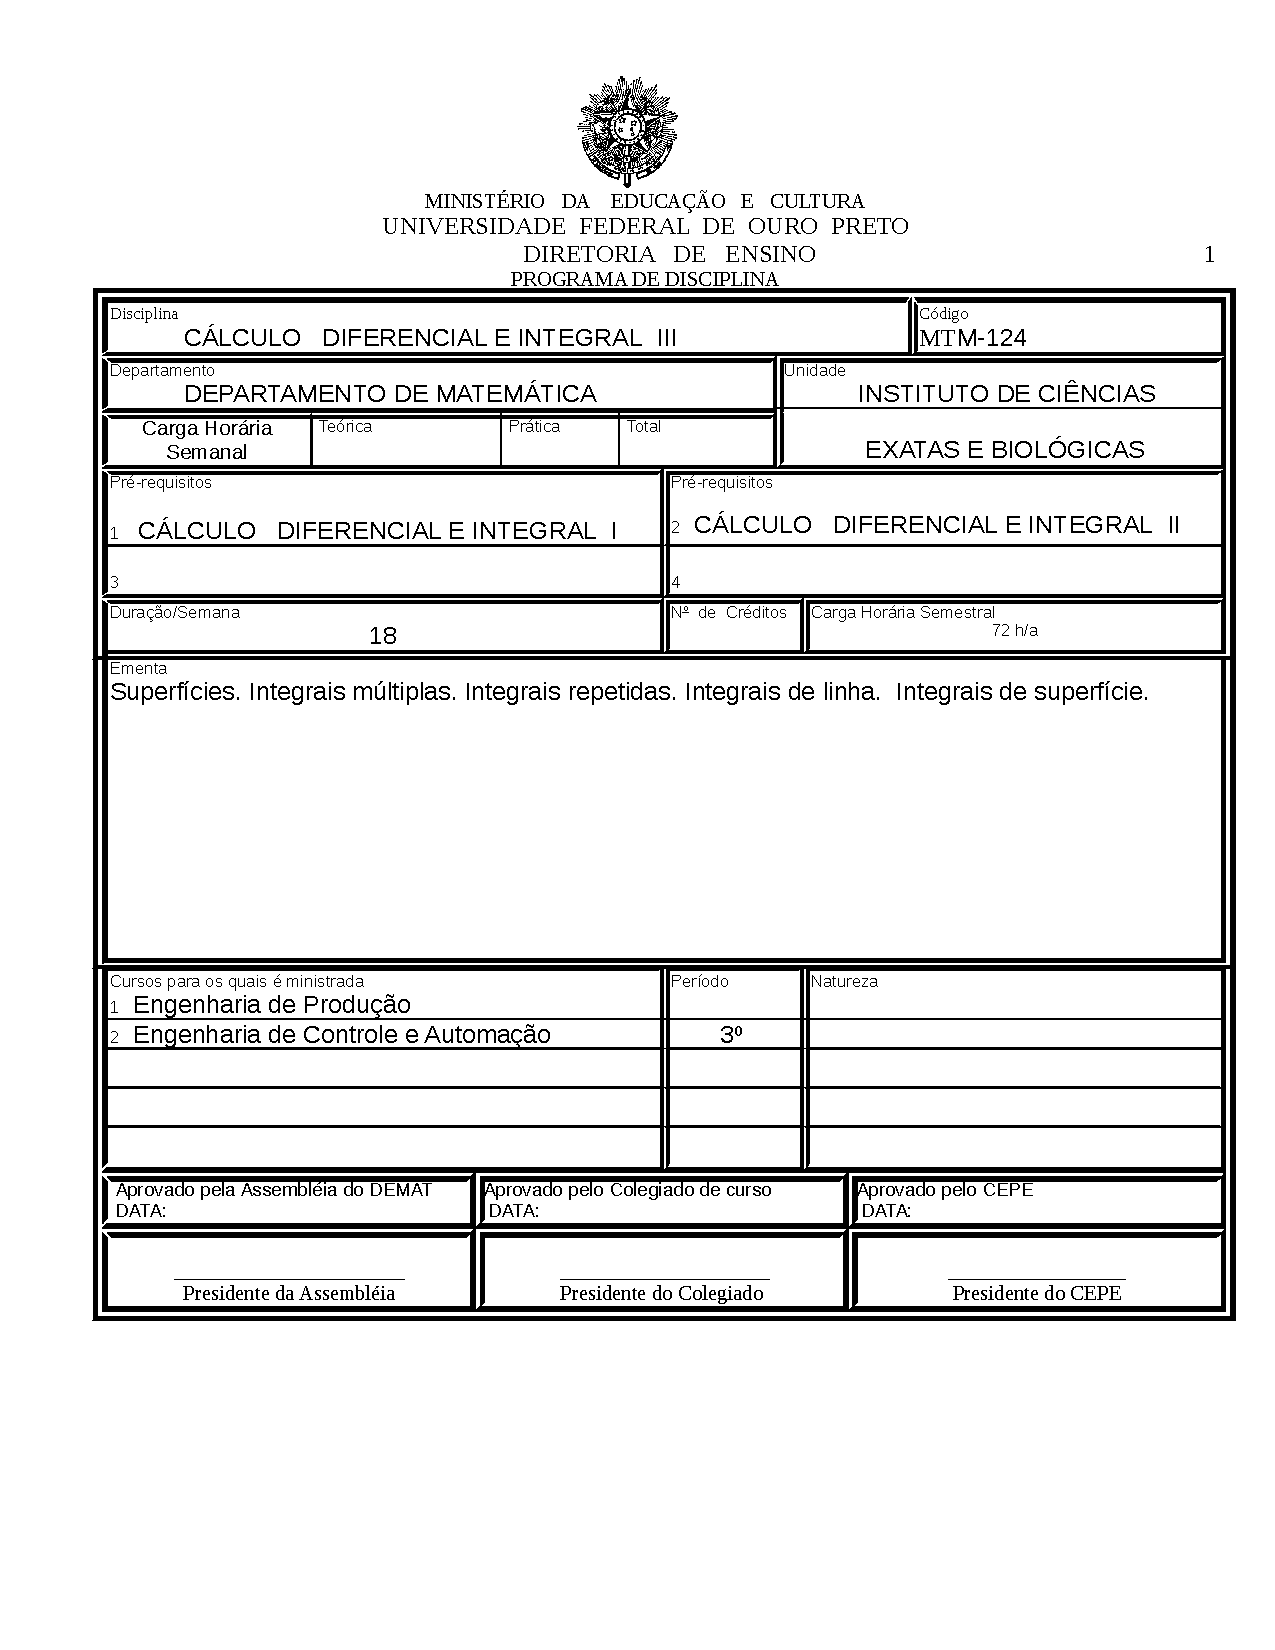
\includegraphics[scale=0.7]{capitulos/anexo1-programas-disciplina/p35.pdf}
	%	\caption{Disciplina do primeiro semestre}
\end{figure}

% quarto semestre
\begin{figure}[p]
	\centering 
	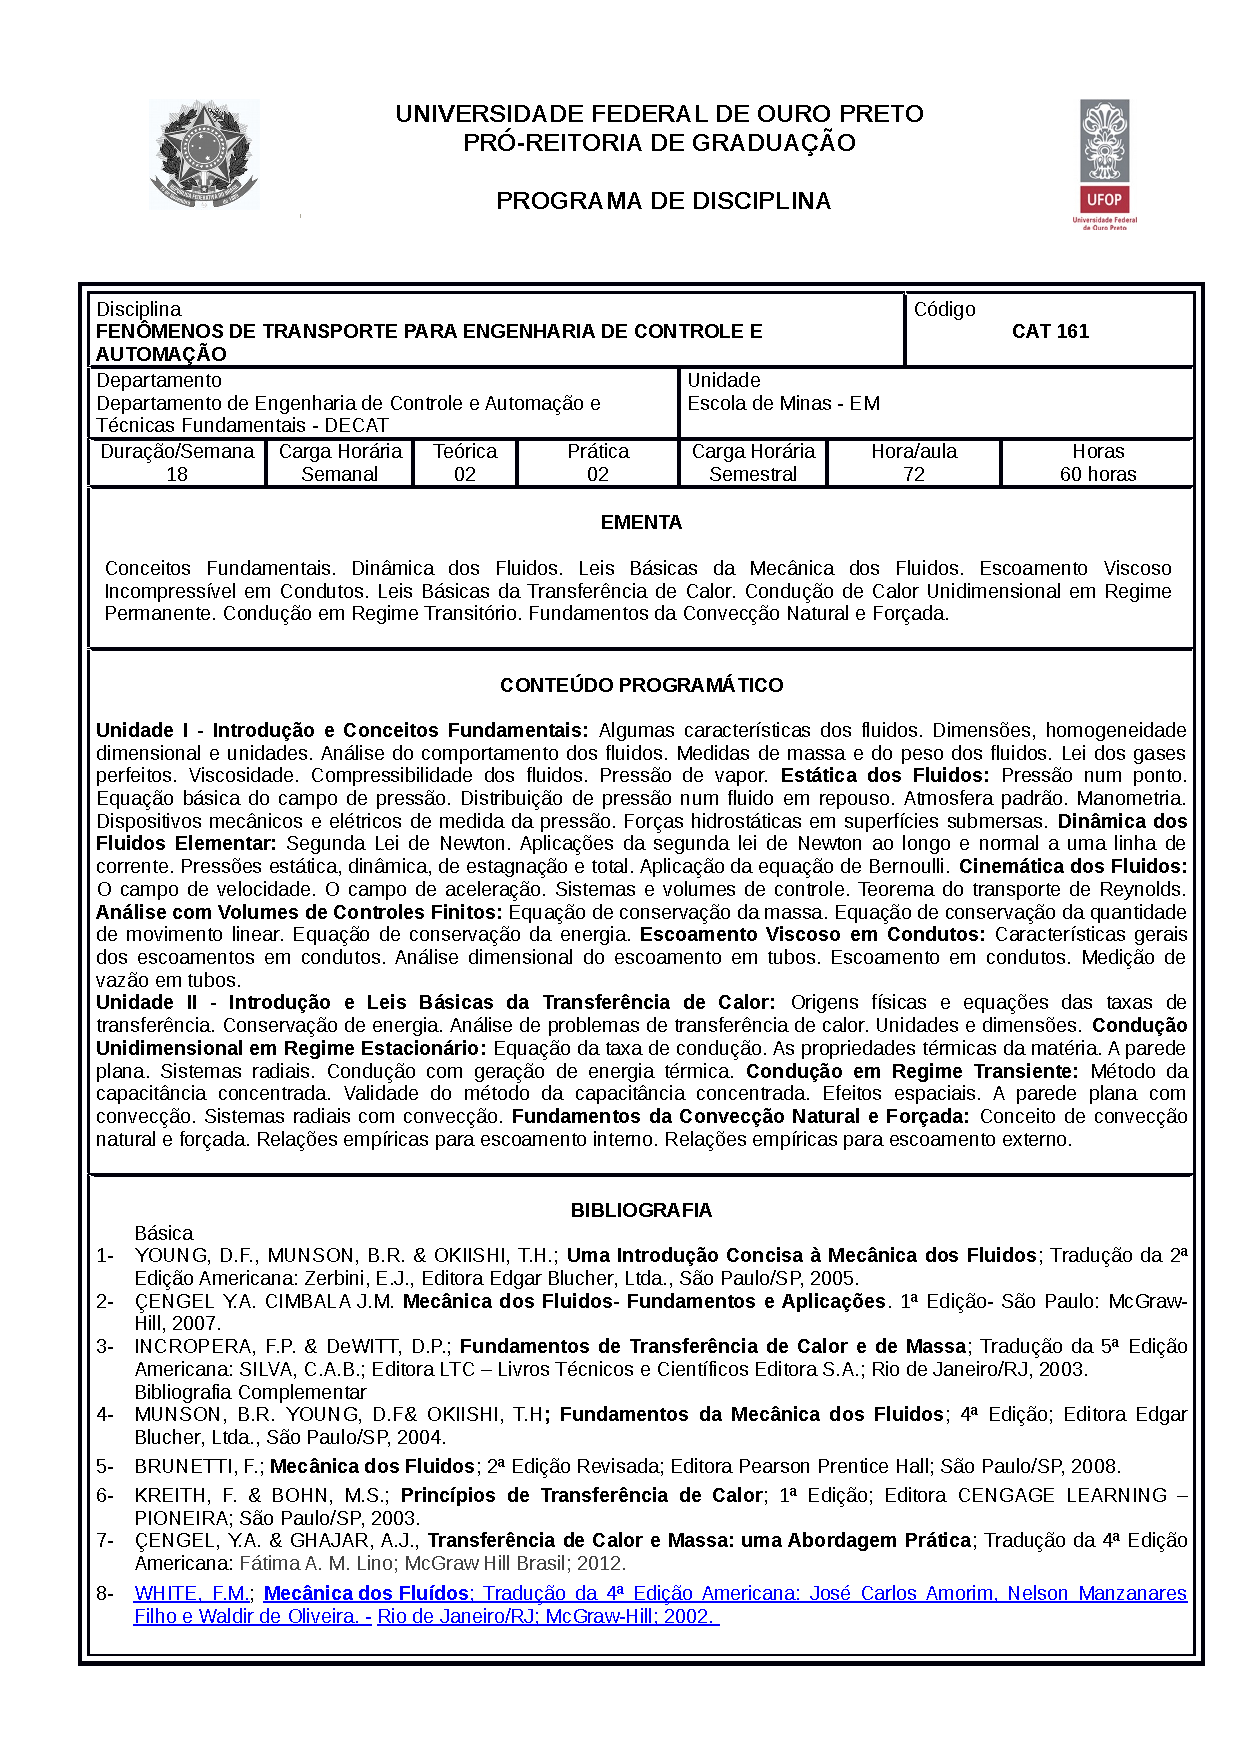
\includegraphics[scale=0.7]{capitulos/anexo1-programas-disciplina/p41.pdf}
	%	\caption{Disciplina do primeiro semestre}
\end{figure}

\begin{figure}[p]
	\centering 
	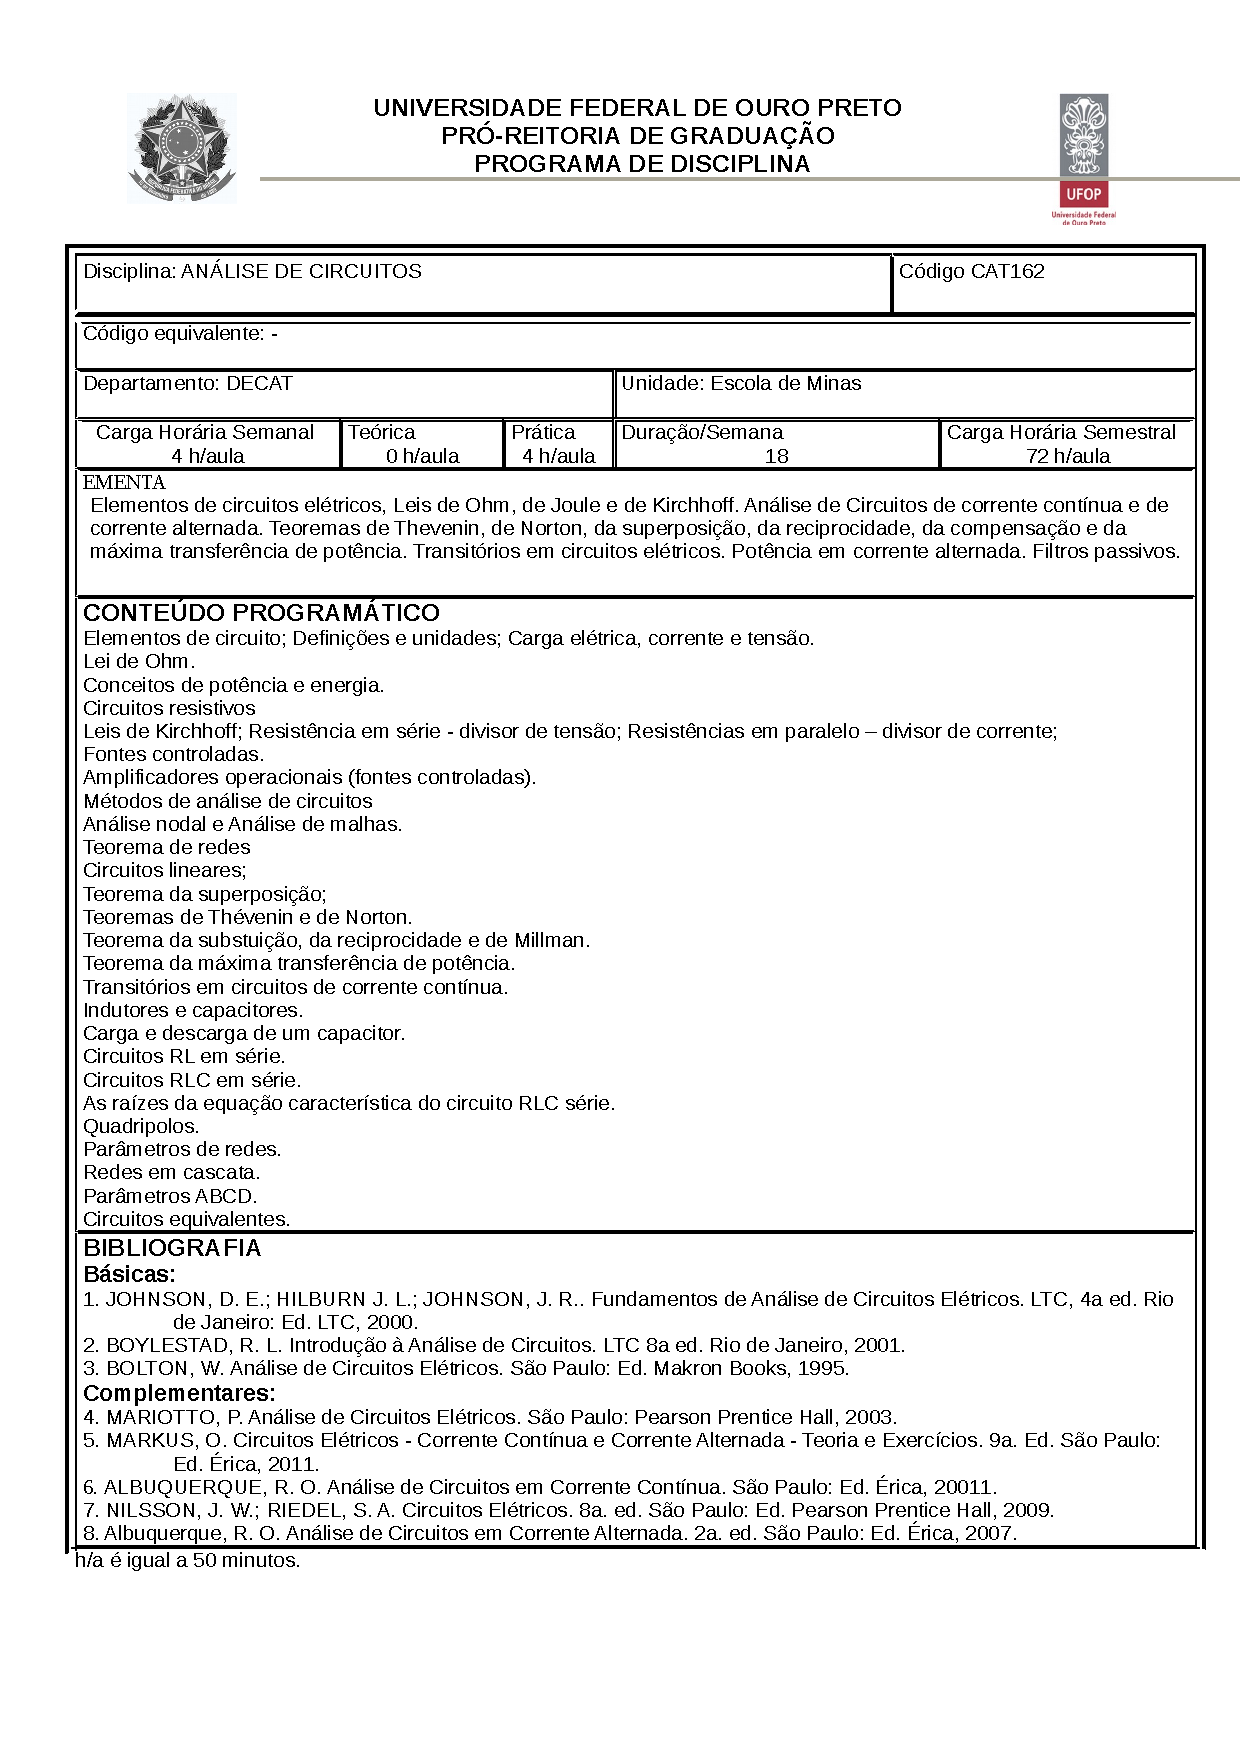
\includegraphics[scale=0.7]{capitulos/anexo1-programas-disciplina/p42.pdf}
	%	\caption{Disciplina do primeiro semestre}
\end{figure}

\begin{figure}[p]
	\centering 
	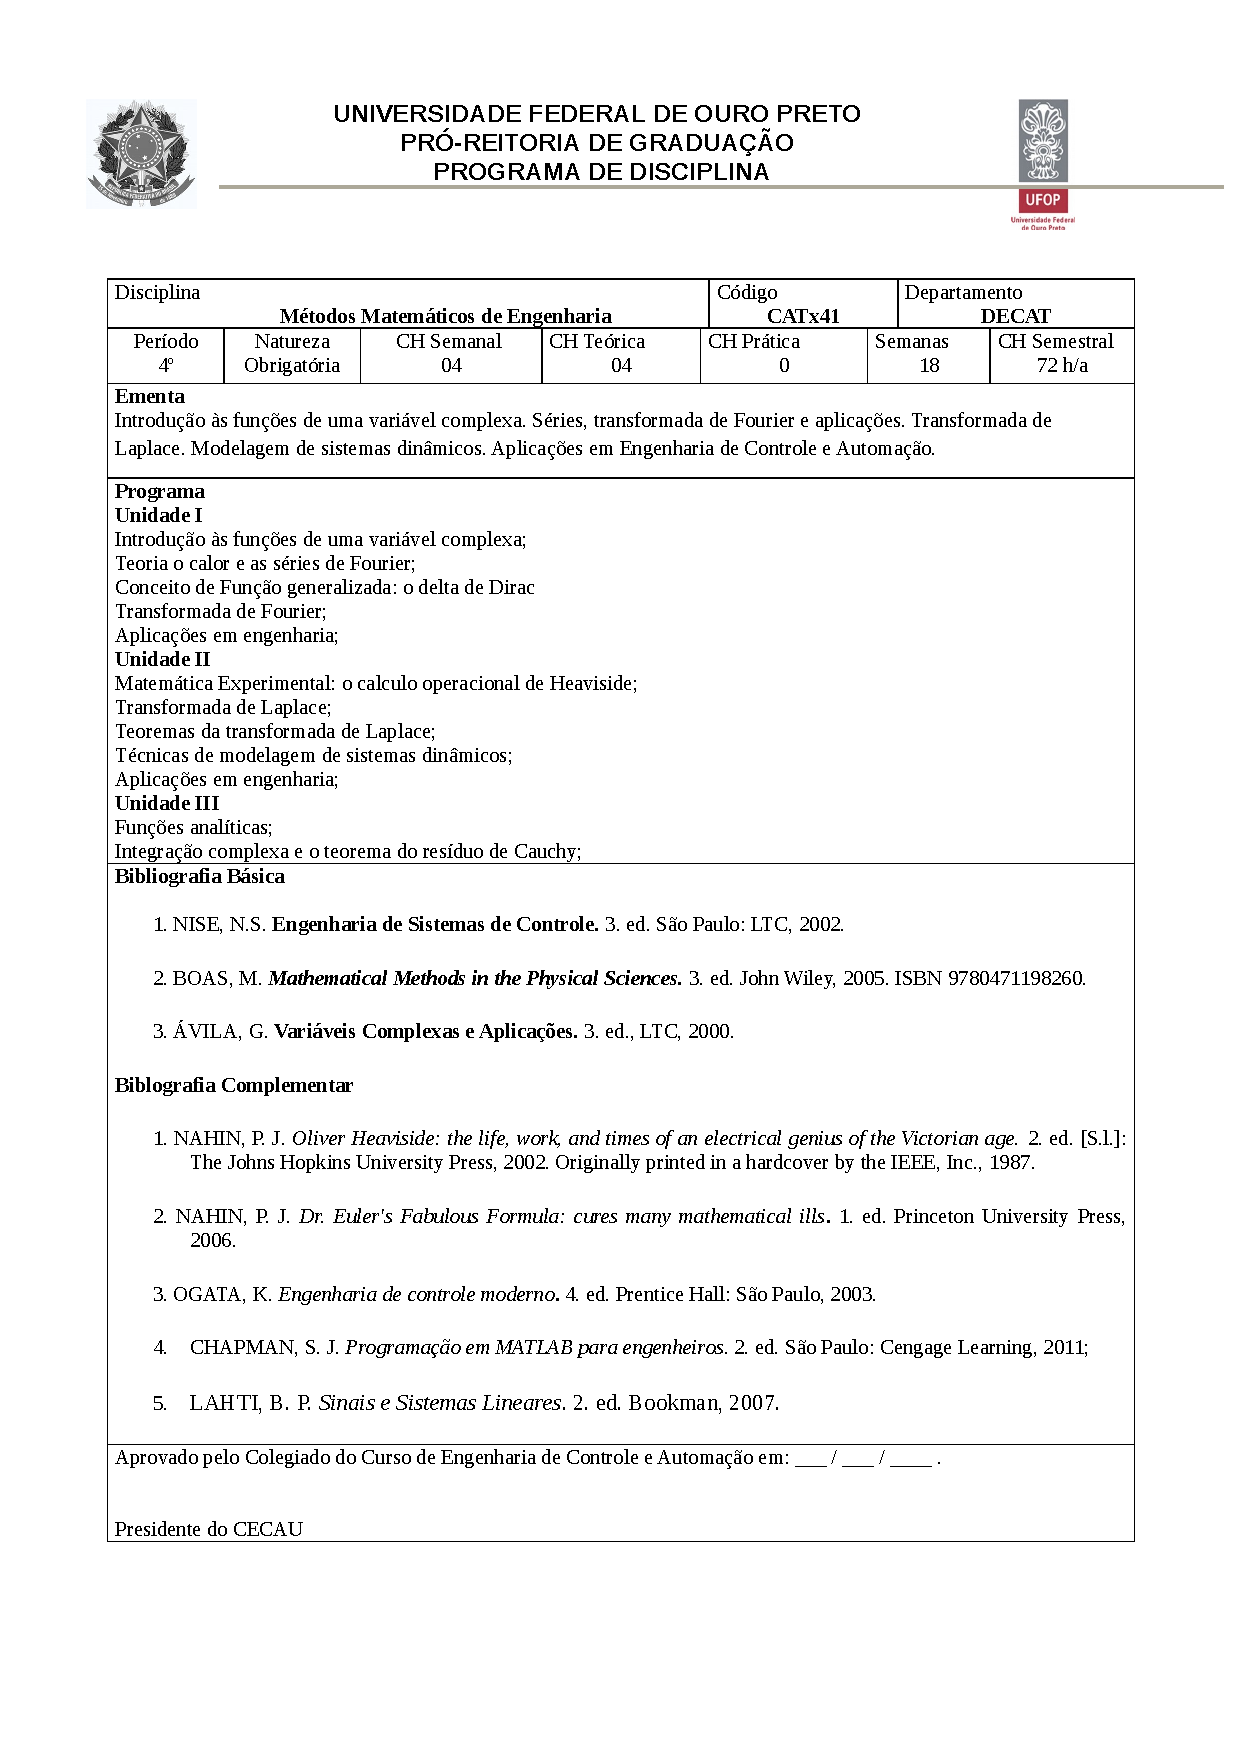
\includegraphics[scale=0.7]{capitulos/anexo1-programas-disciplina/p43.pdf}
	%	\caption{Disciplina do primeiro semestre}
\end{figure}

\begin{figure}[p]
	\centering 
	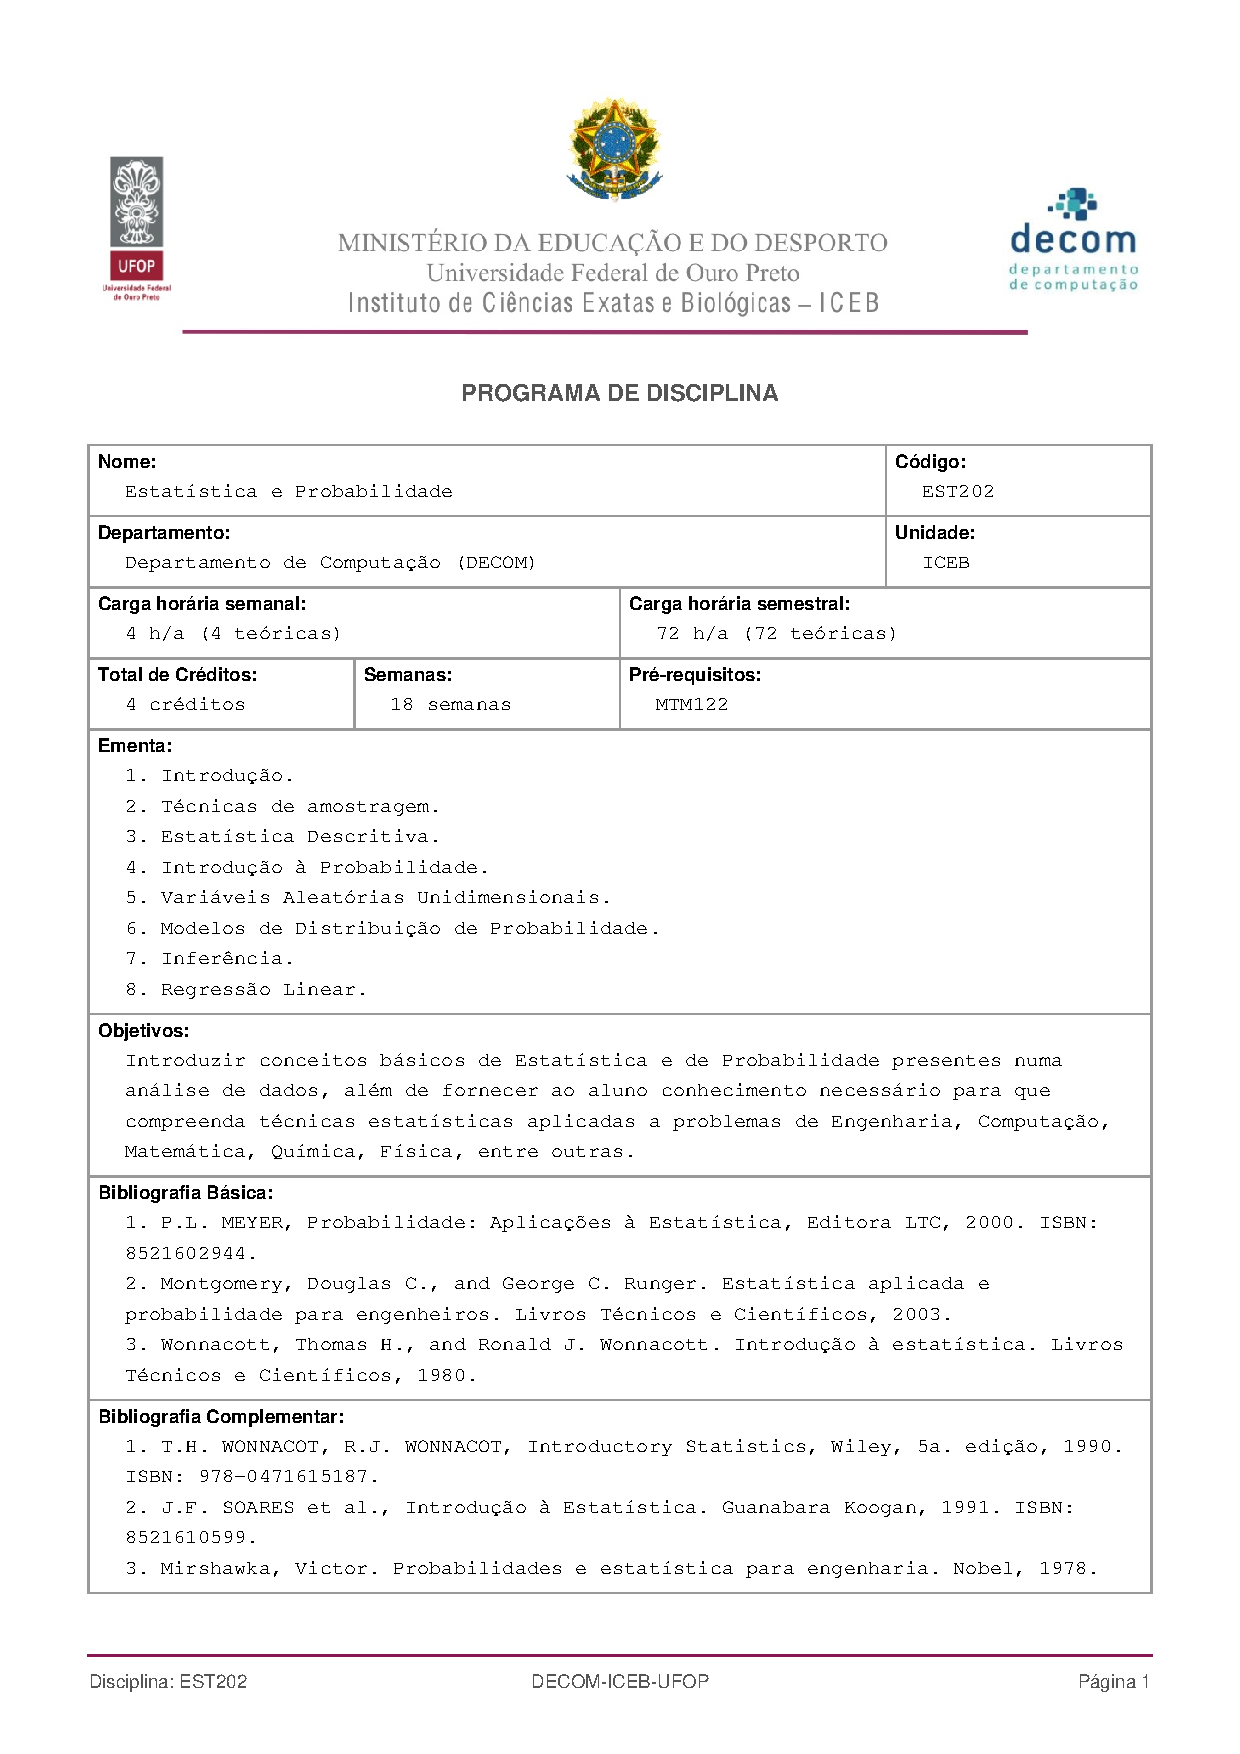
\includegraphics[scale=0.7]{capitulos/anexo1-programas-disciplina/p44.pdf}
	%	\caption{Disciplina do primeiro semestre}
\end{figure}

\begin{figure}[p]
	\centering 
	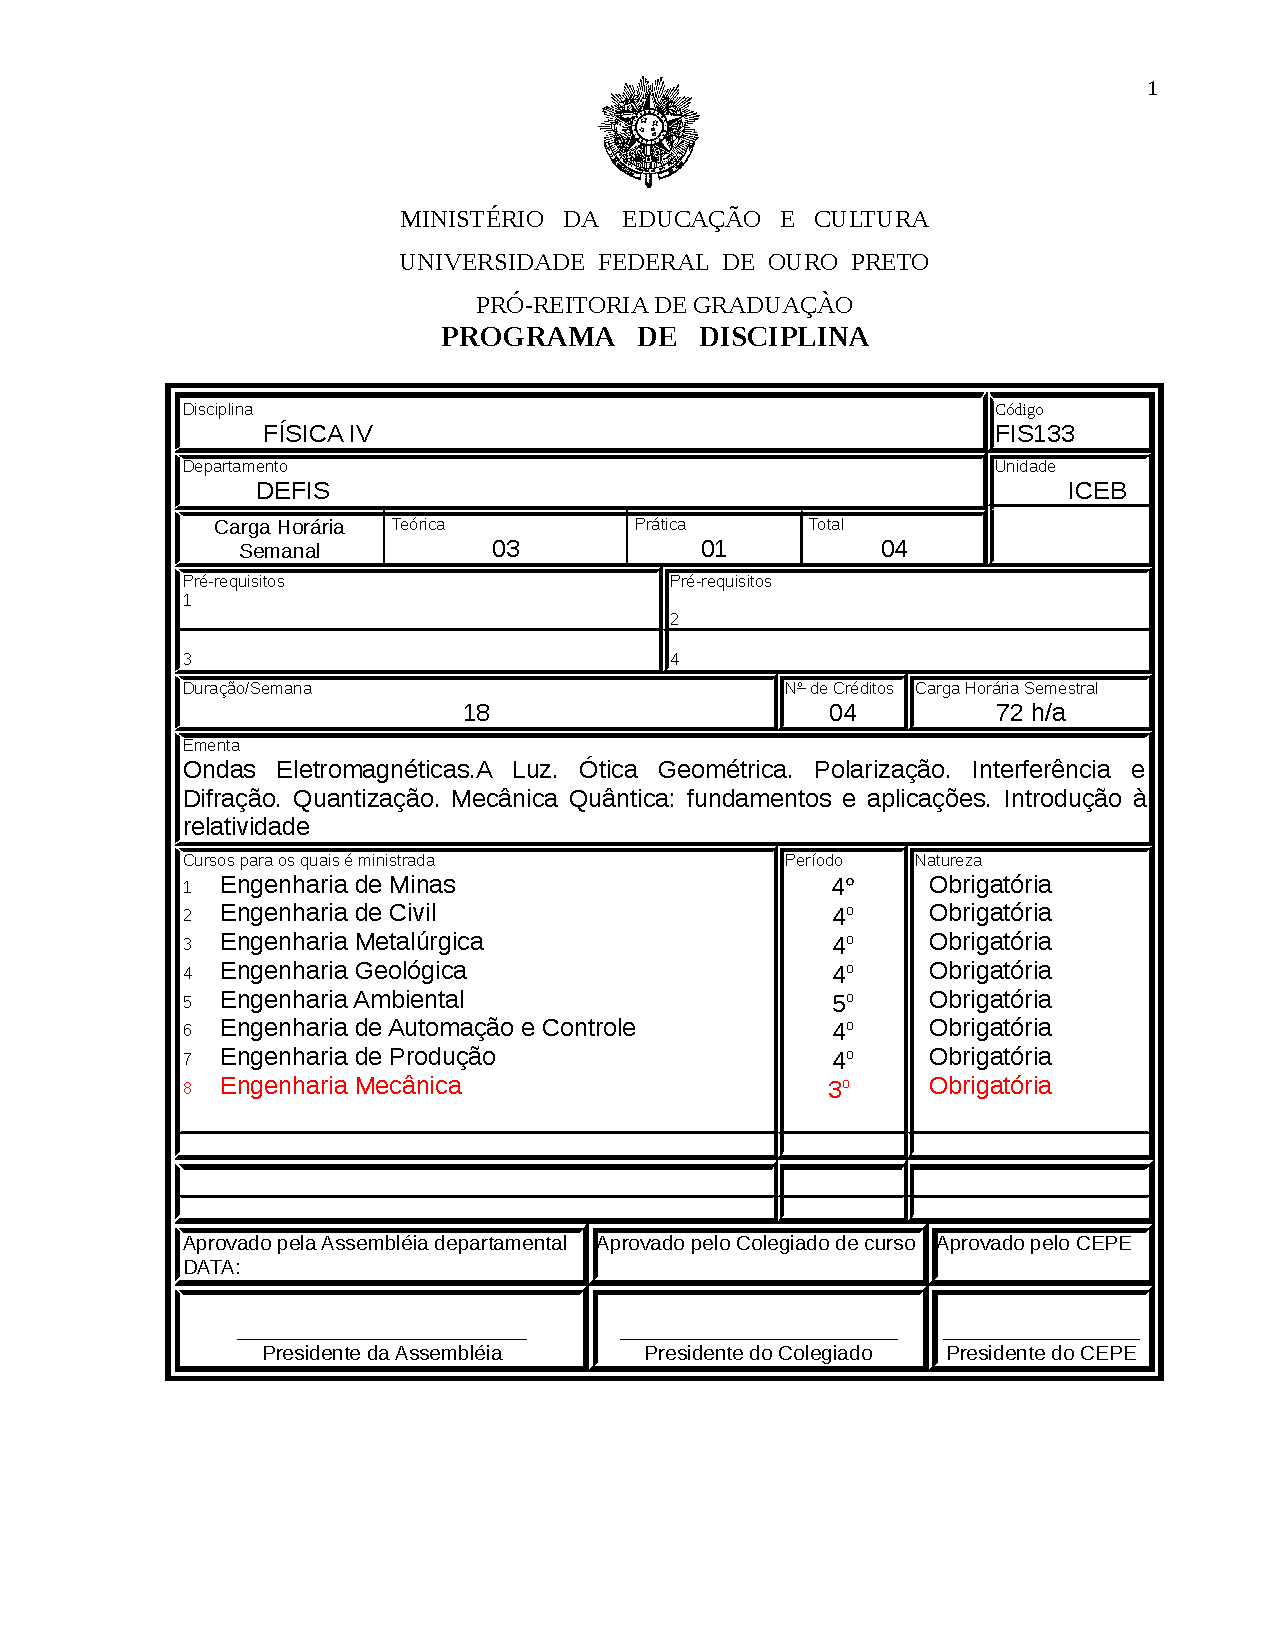
\includegraphics[scale=0.7]{capitulos/anexo1-programas-disciplina/p45.pdf}
	%	\caption{Disciplina do primeiro semestre}
\end{figure}

% quinto semestre

\begin{figure}[p]
	\centering 
	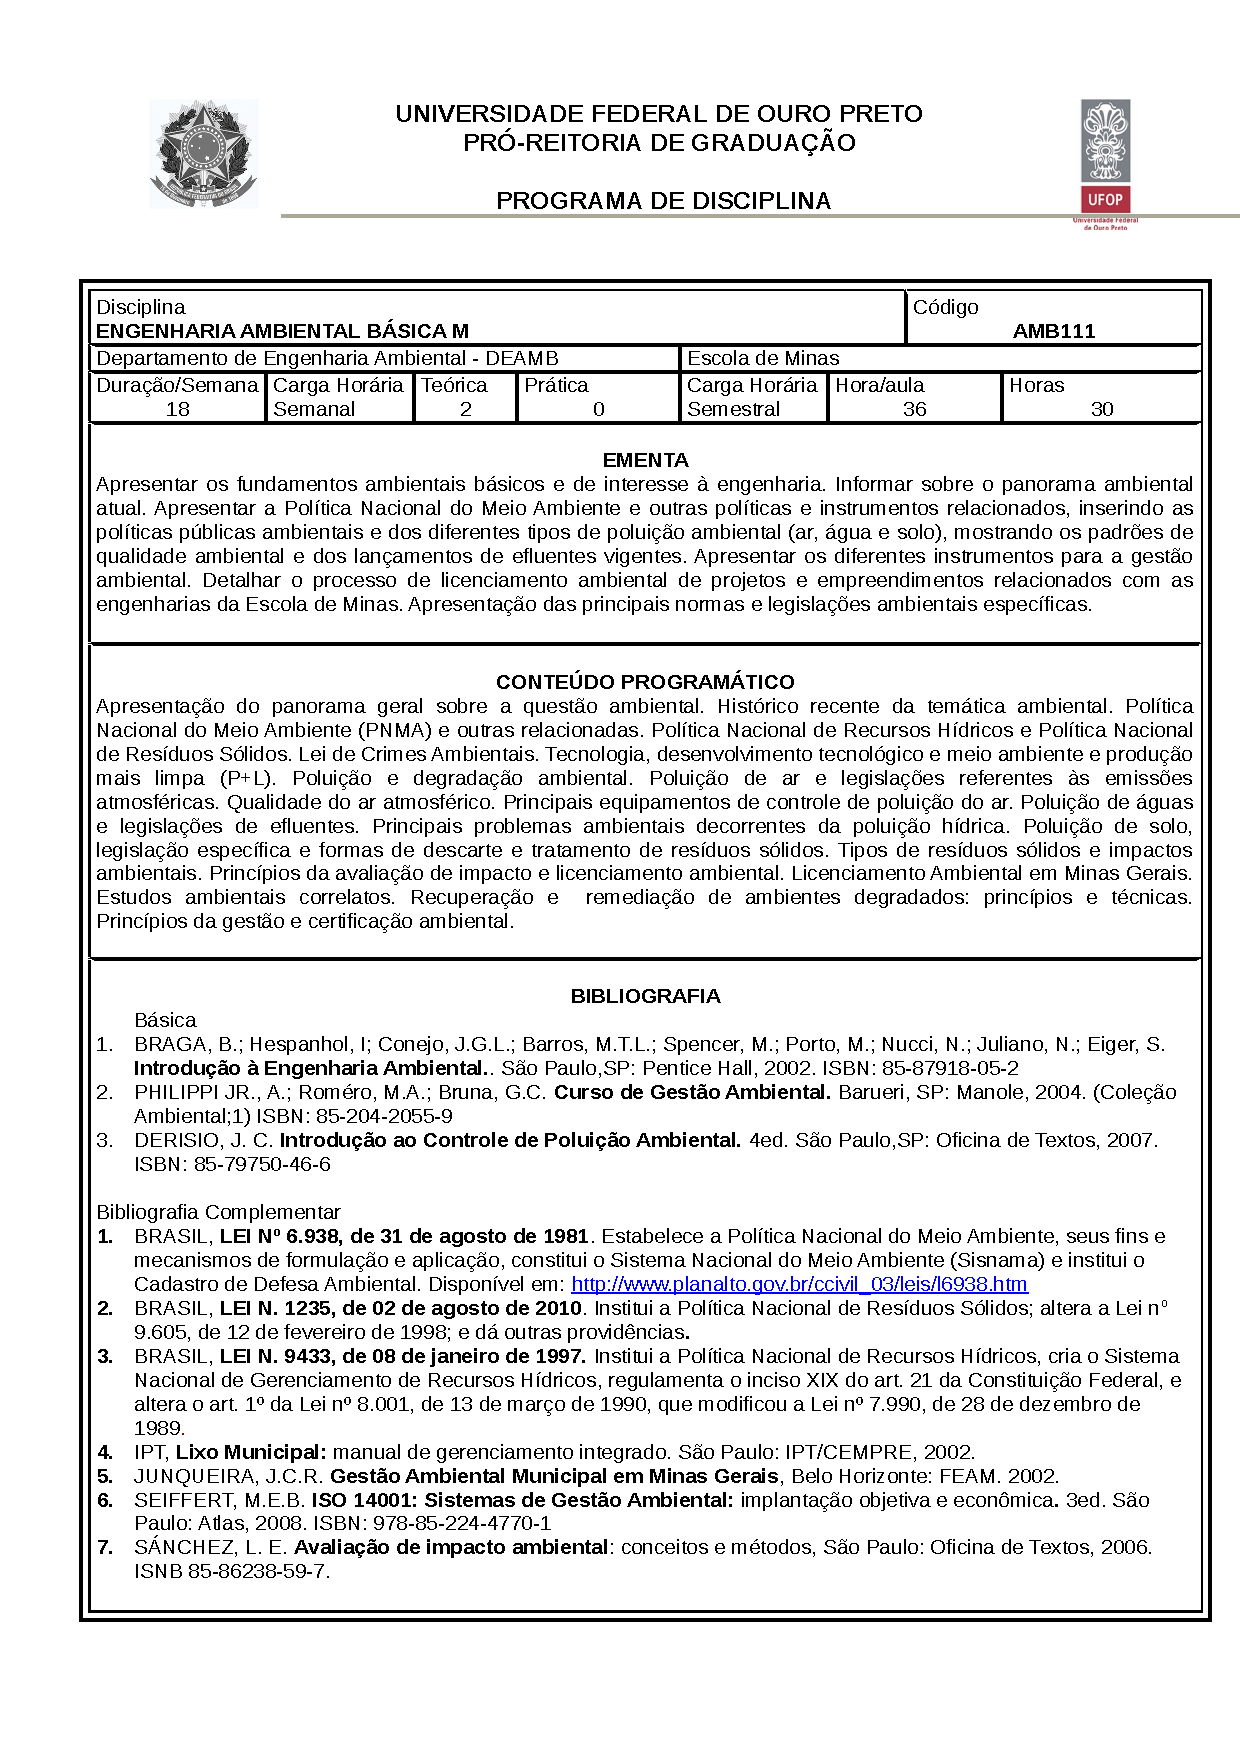
\includegraphics[scale=0.7]{capitulos/anexo1-programas-disciplina/p51.pdf}
	%	\caption{Disciplina do primeiro semestre}
\end{figure}

\begin{figure}[p]
	\centering 
	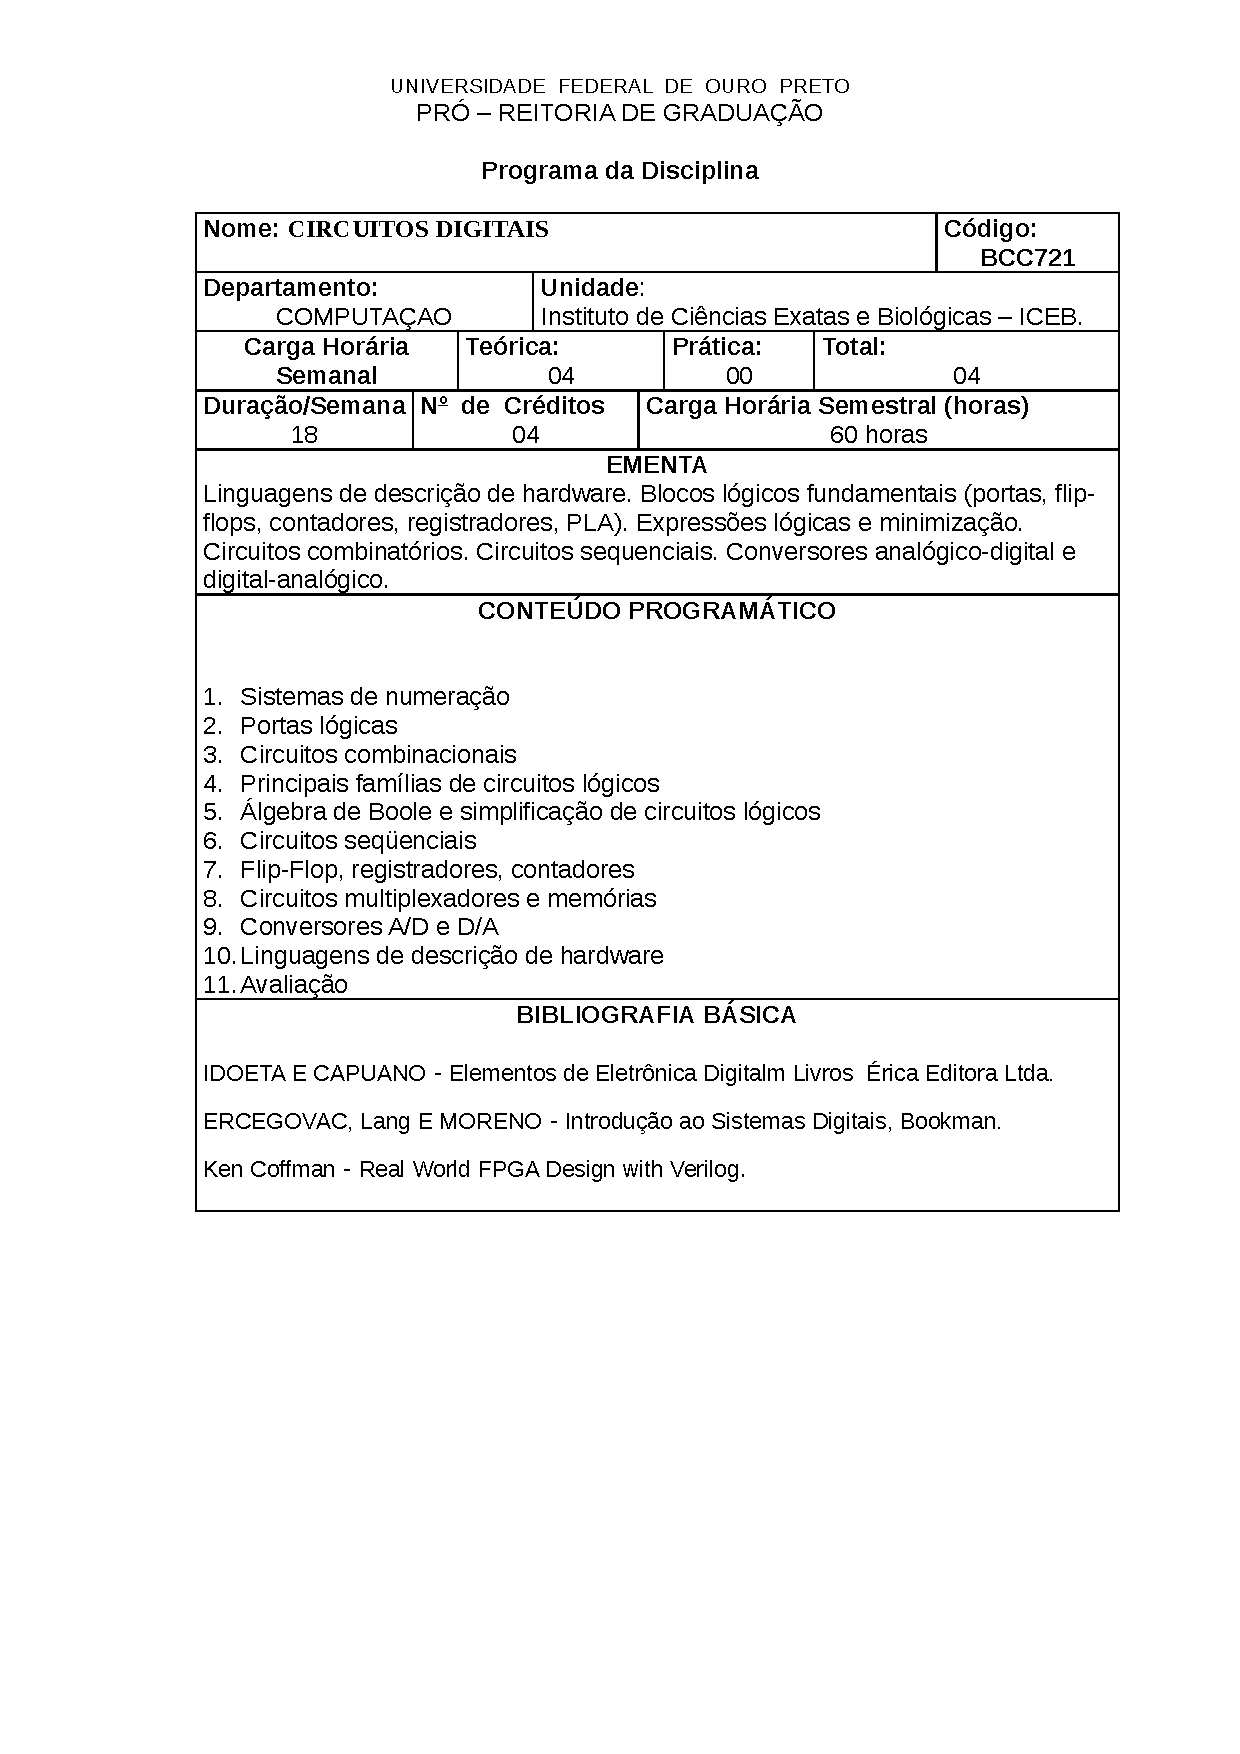
\includegraphics[scale=0.7]{capitulos/anexo1-programas-disciplina/p52.pdf}
	%	\caption{Disciplina do primeiro semestre}
\end{figure}

\begin{figure}[p]
	\centering 
	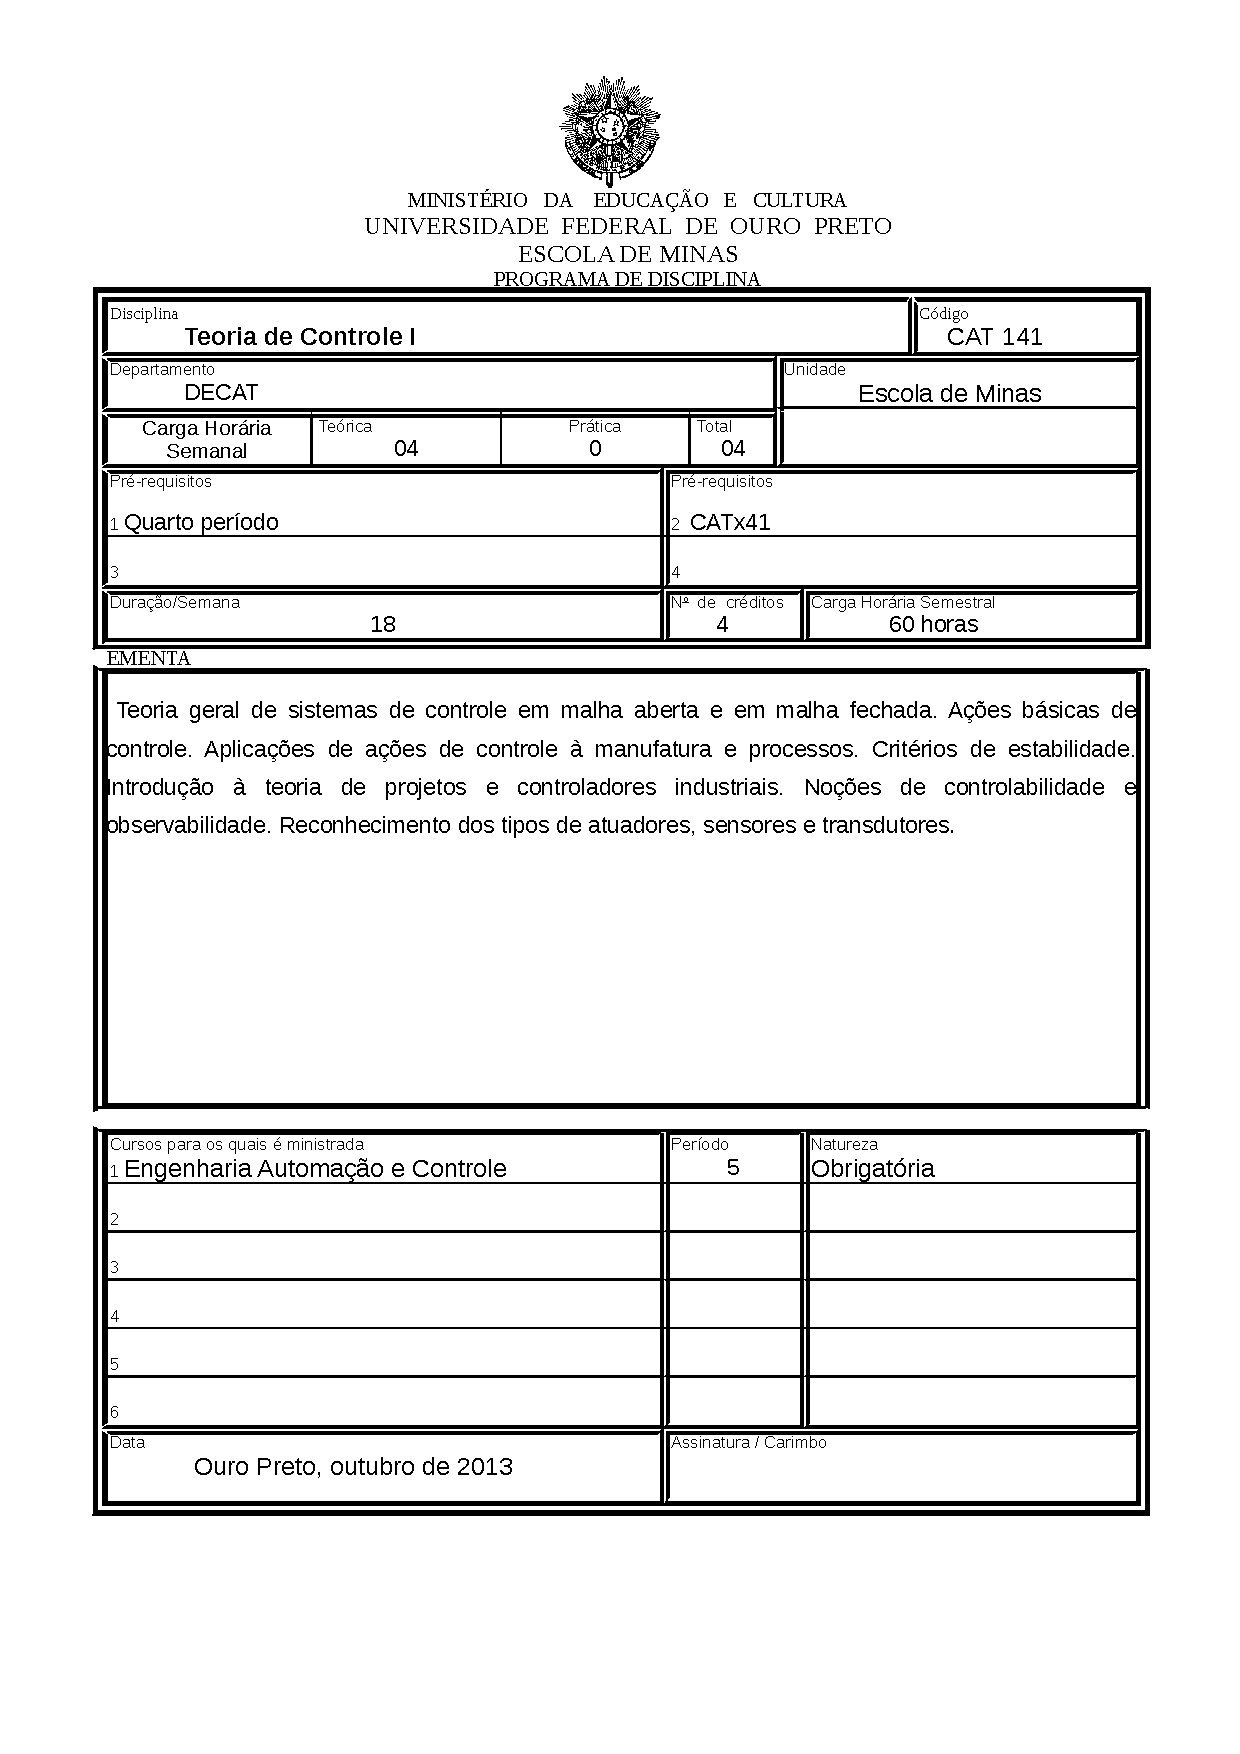
\includegraphics[scale=0.7]{capitulos/anexo1-programas-disciplina/p53.pdf}
	%	\caption{Disciplina do primeiro semestre}
\end{figure}

\begin{figure}[p]
	\centering 
	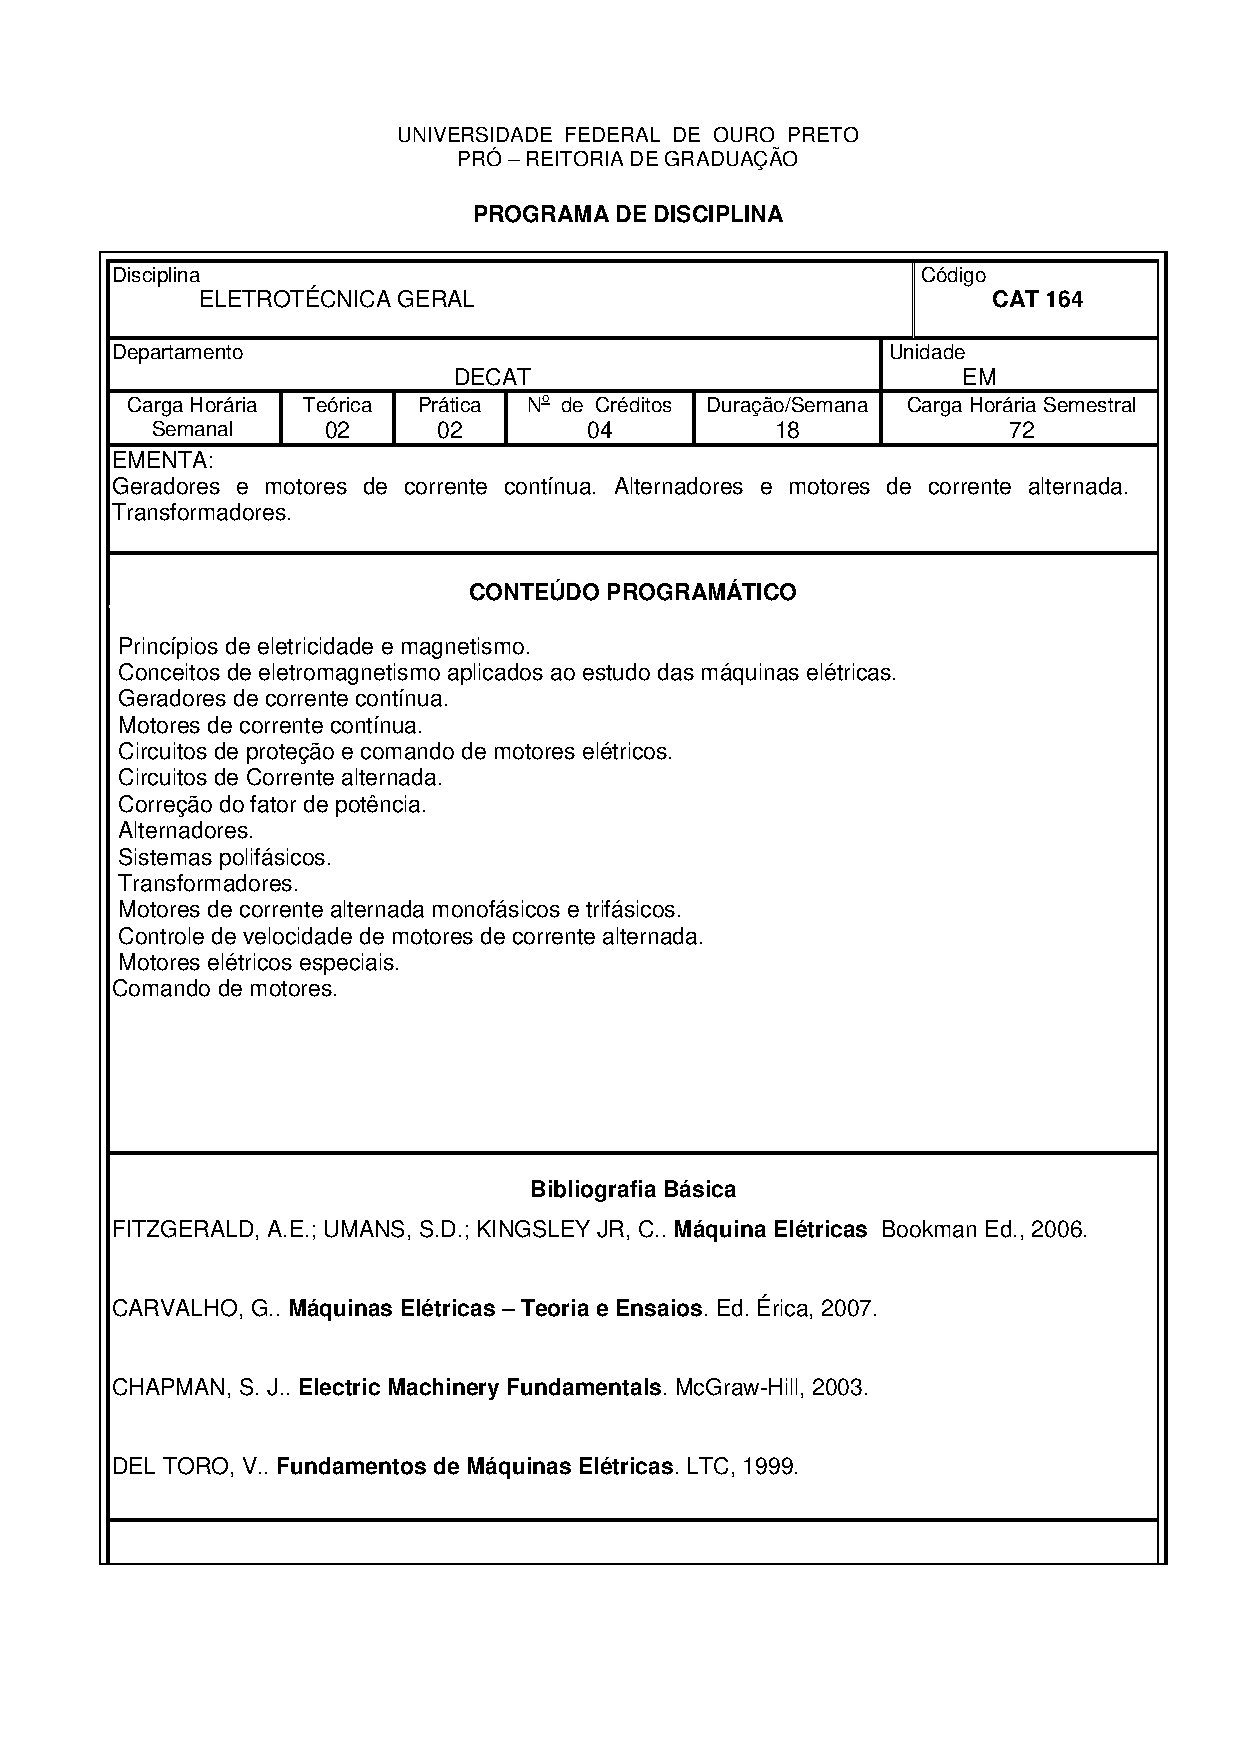
\includegraphics[scale=0.7]{capitulos/anexo1-programas-disciplina/p54.pdf}
	%	\caption{Disciplina do primeiro semestre}
\end{figure}

\begin{figure}[p]
	\centering 
	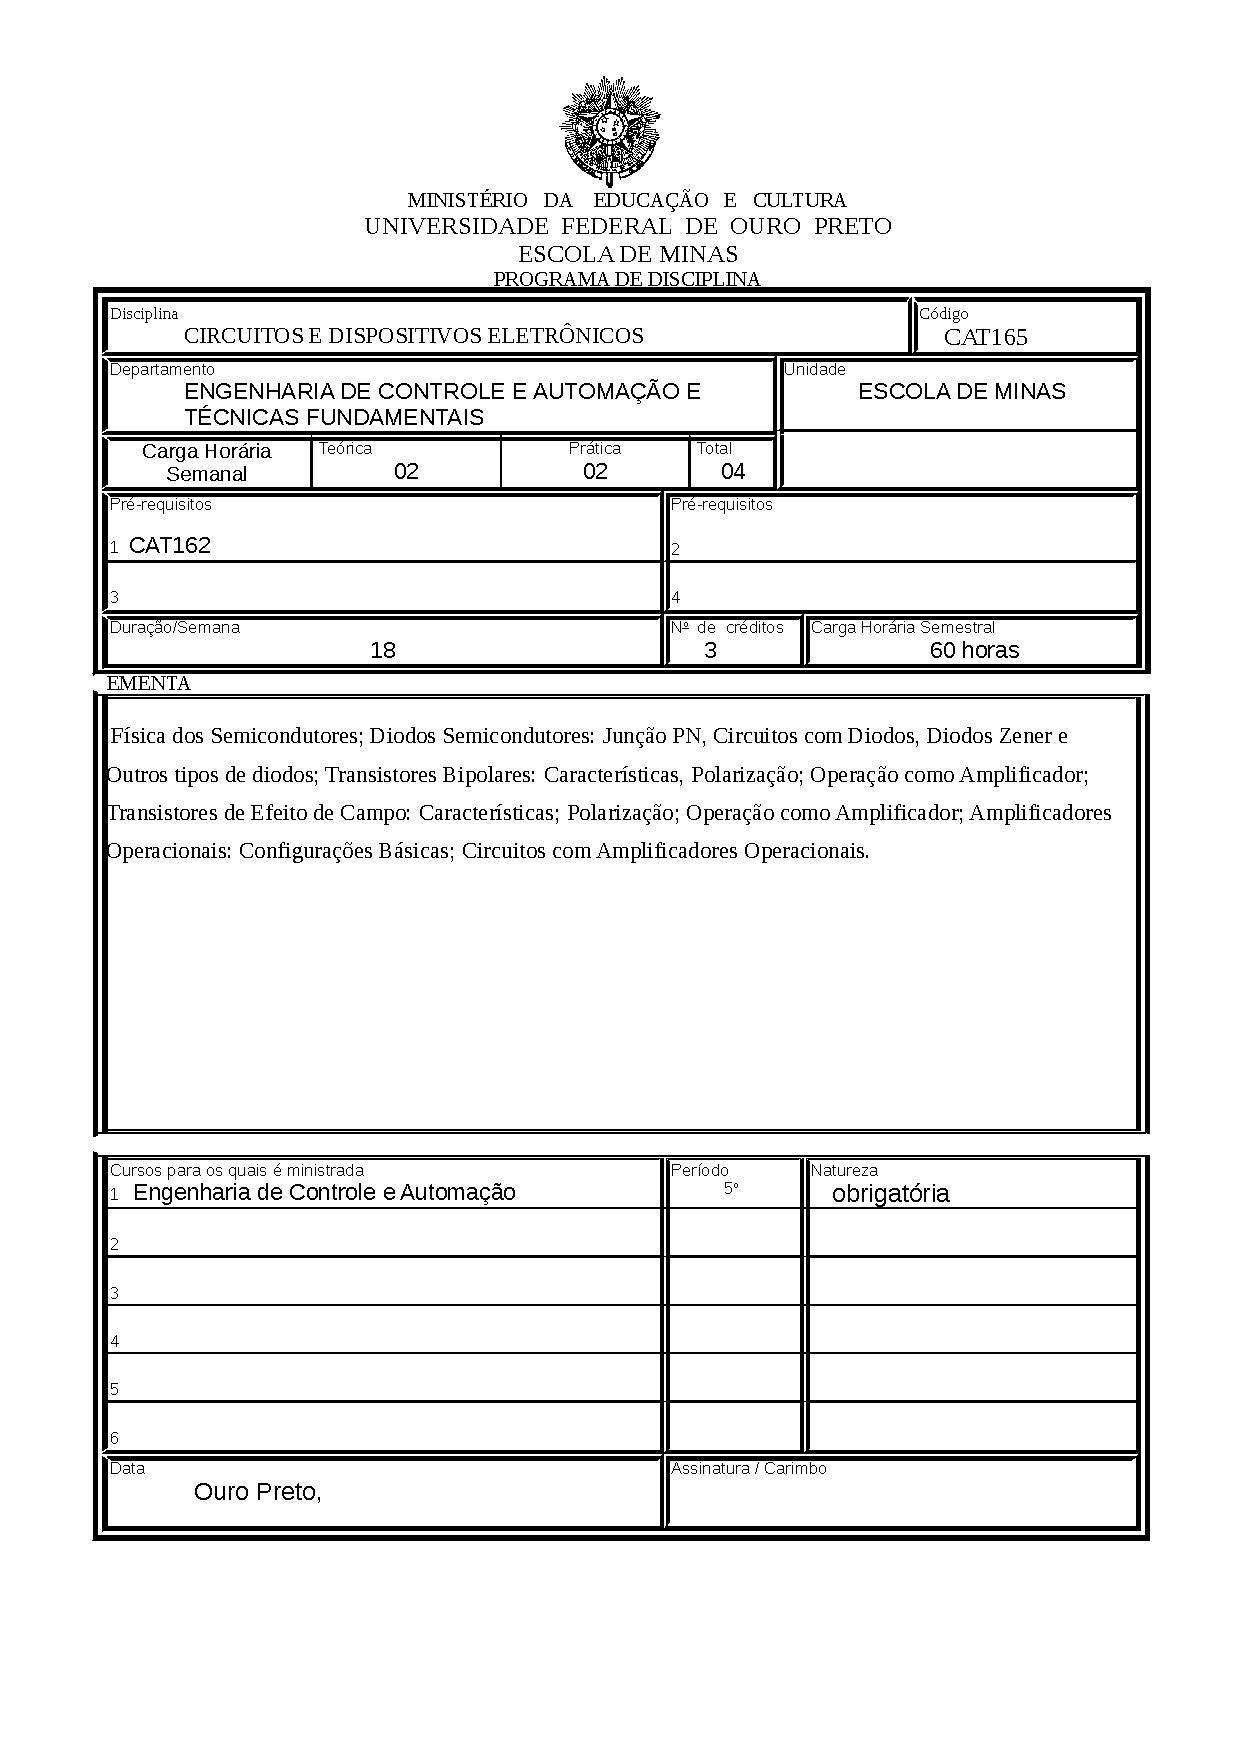
\includegraphics[scale=0.7]{capitulos/anexo1-programas-disciplina/p55.pdf}
	%	\caption{Disciplina do primeiro semestre}
\end{figure}

\begin{figure}[p]
	\centering 
	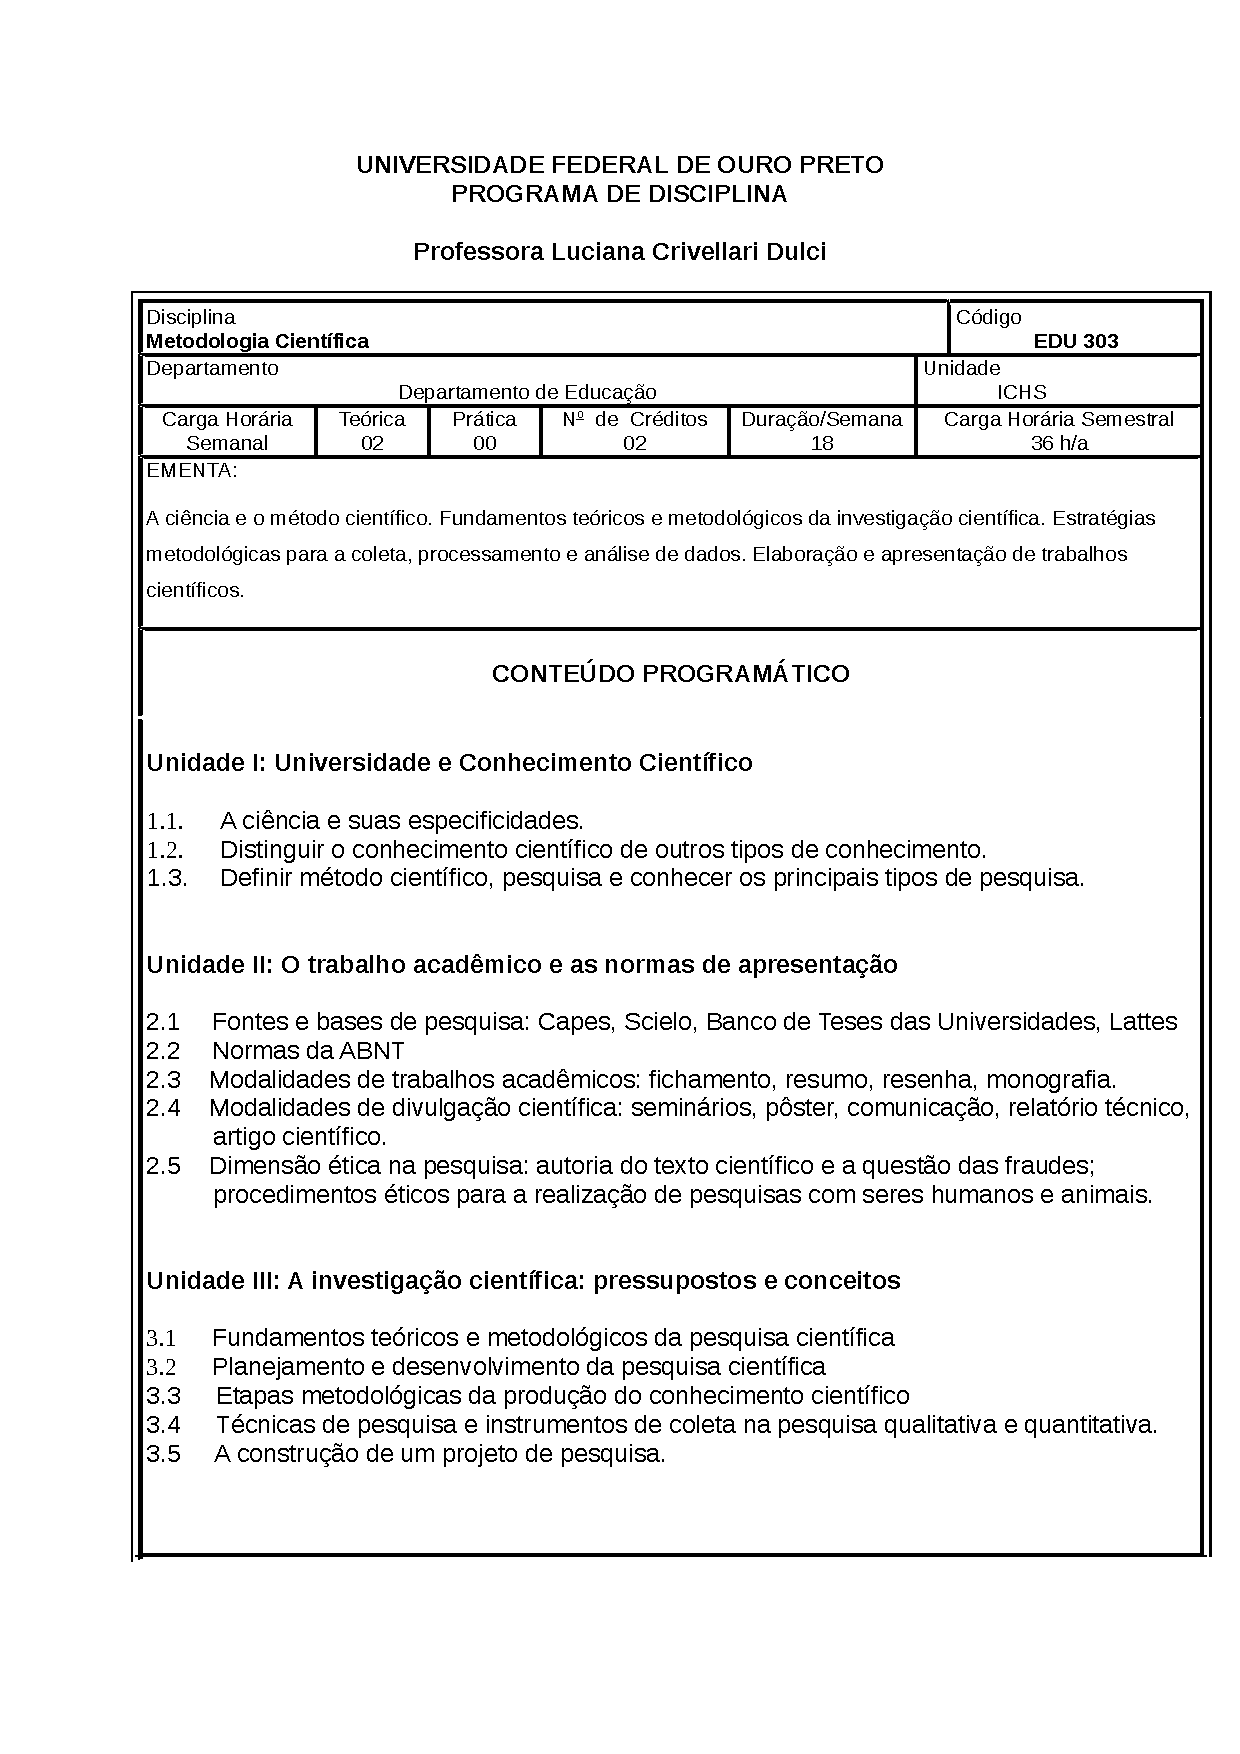
\includegraphics[scale=0.7]{capitulos/anexo1-programas-disciplina/p56.pdf}
	%	\caption{Disciplina do primeiro semestre}
\end{figure}

%sexto semestre
\begin{figure}[p]
	\centering 
	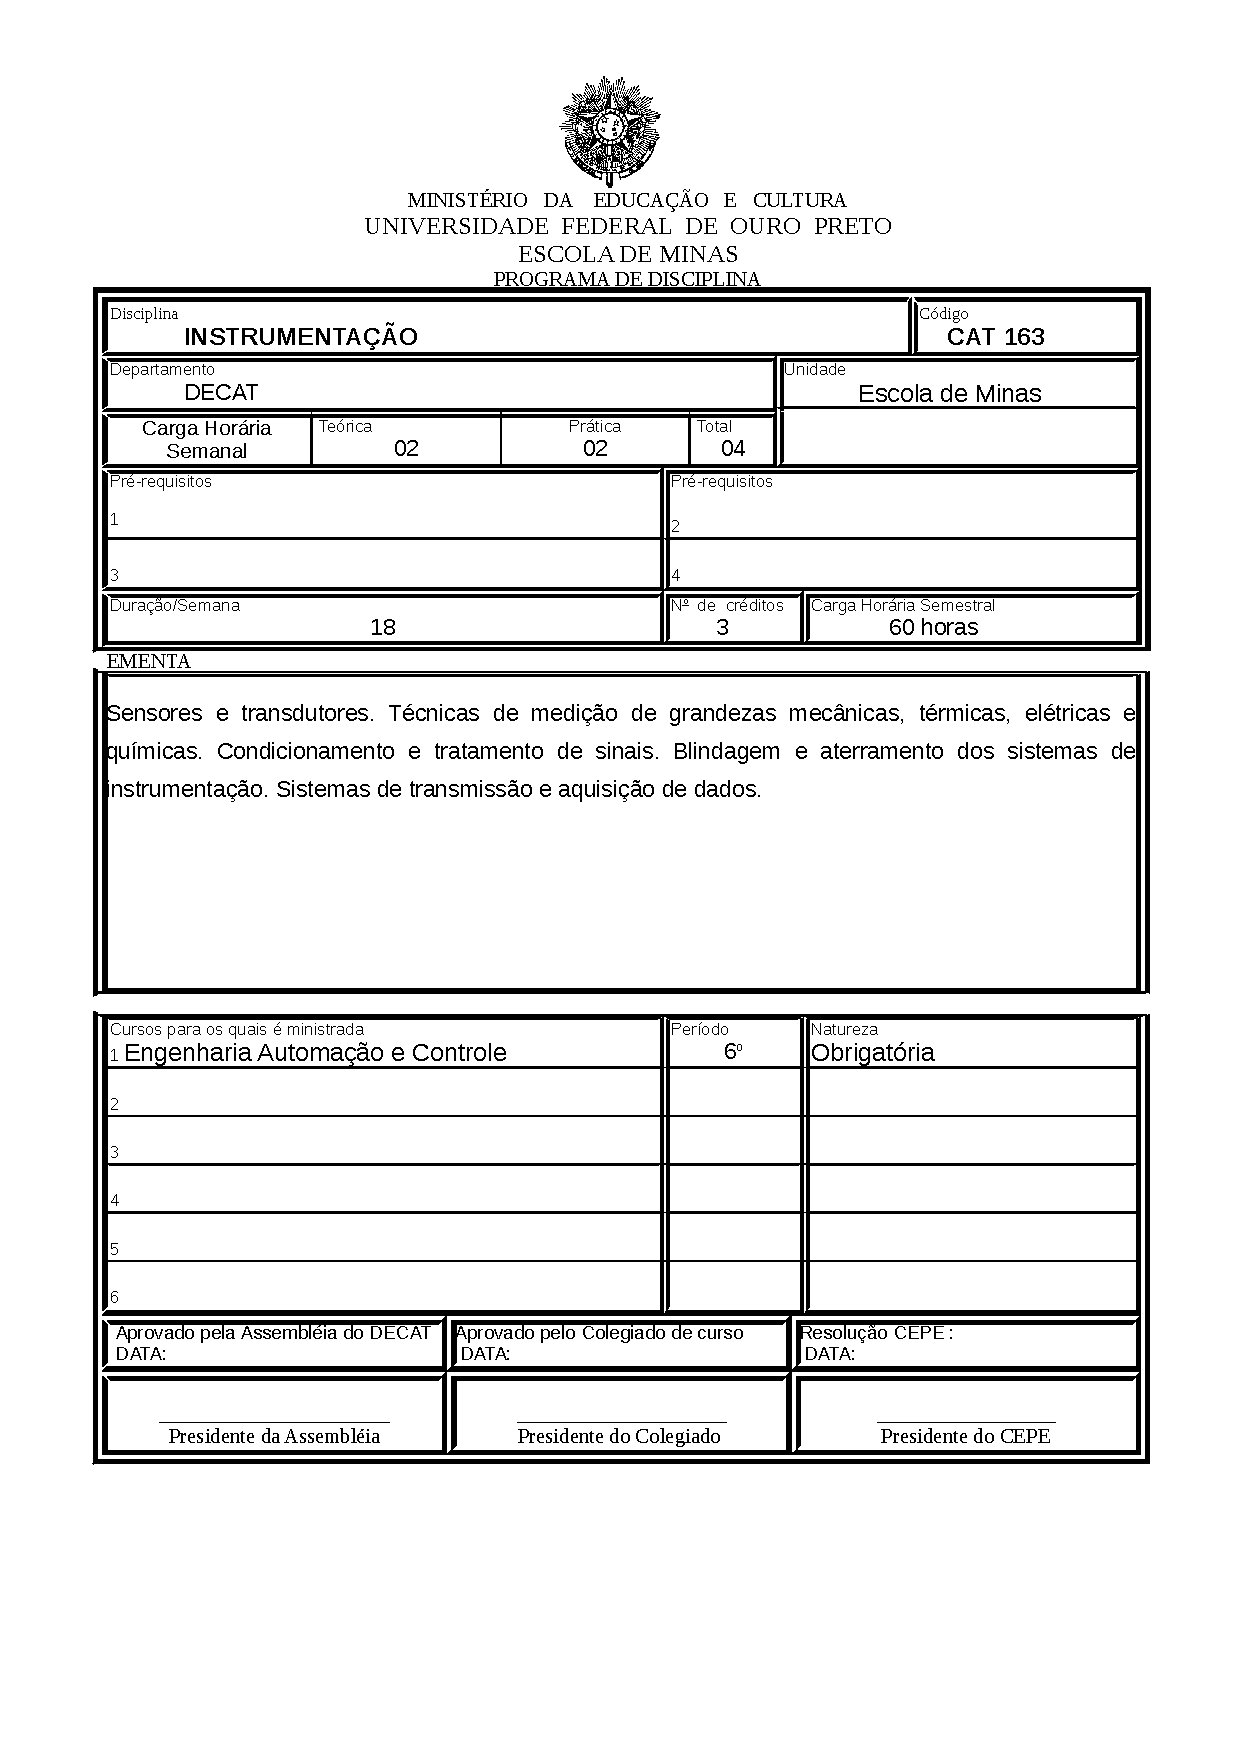
\includegraphics[scale=0.7]{capitulos/anexo1-programas-disciplina/p61.pdf}
	%	\caption{Disciplina do primeiro semestre}
\end{figure}

\begin{figure}[p]
	\centering 
	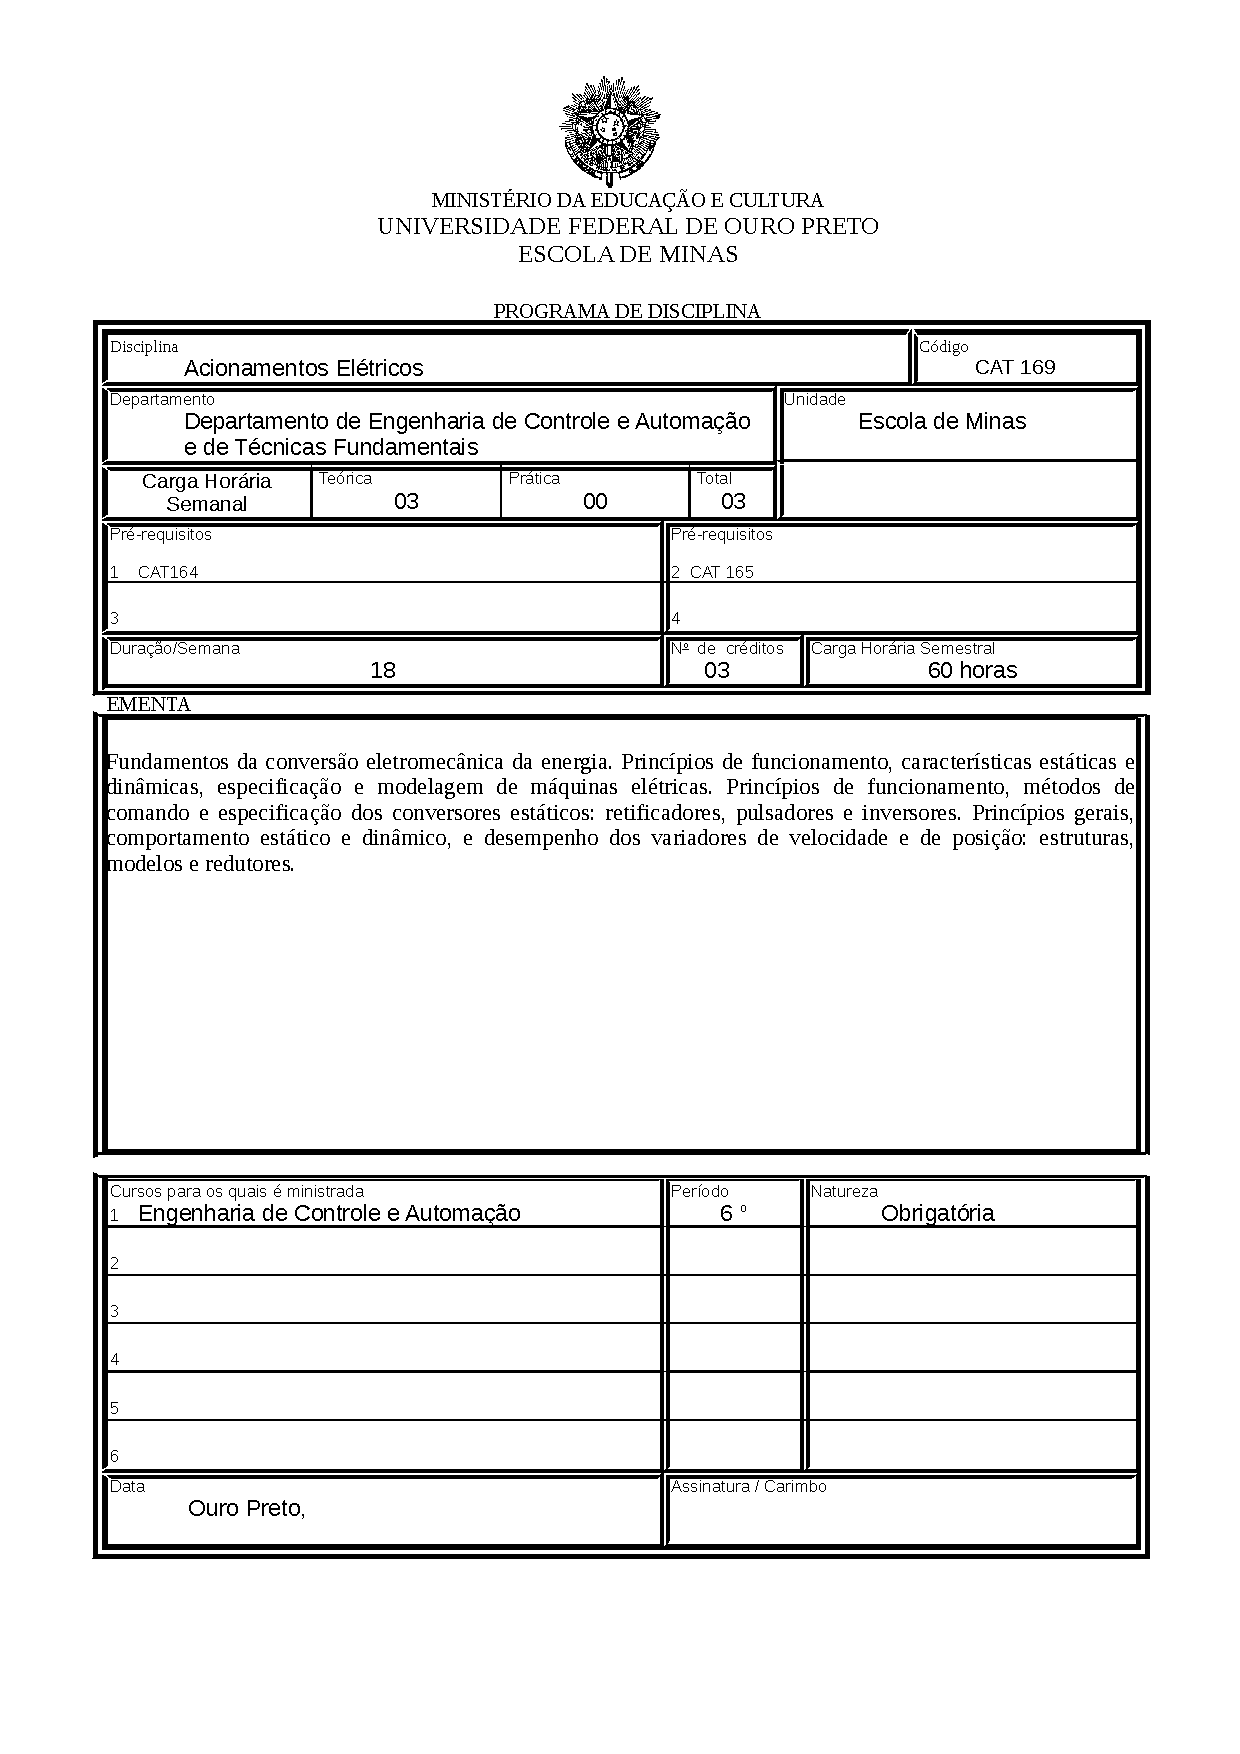
\includegraphics[scale=0.7]{capitulos/anexo1-programas-disciplina/p62.pdf}
	%	\caption{Disciplina do primeiro semestre}
\end{figure}

\begin{figure}[p]
	\centering 
	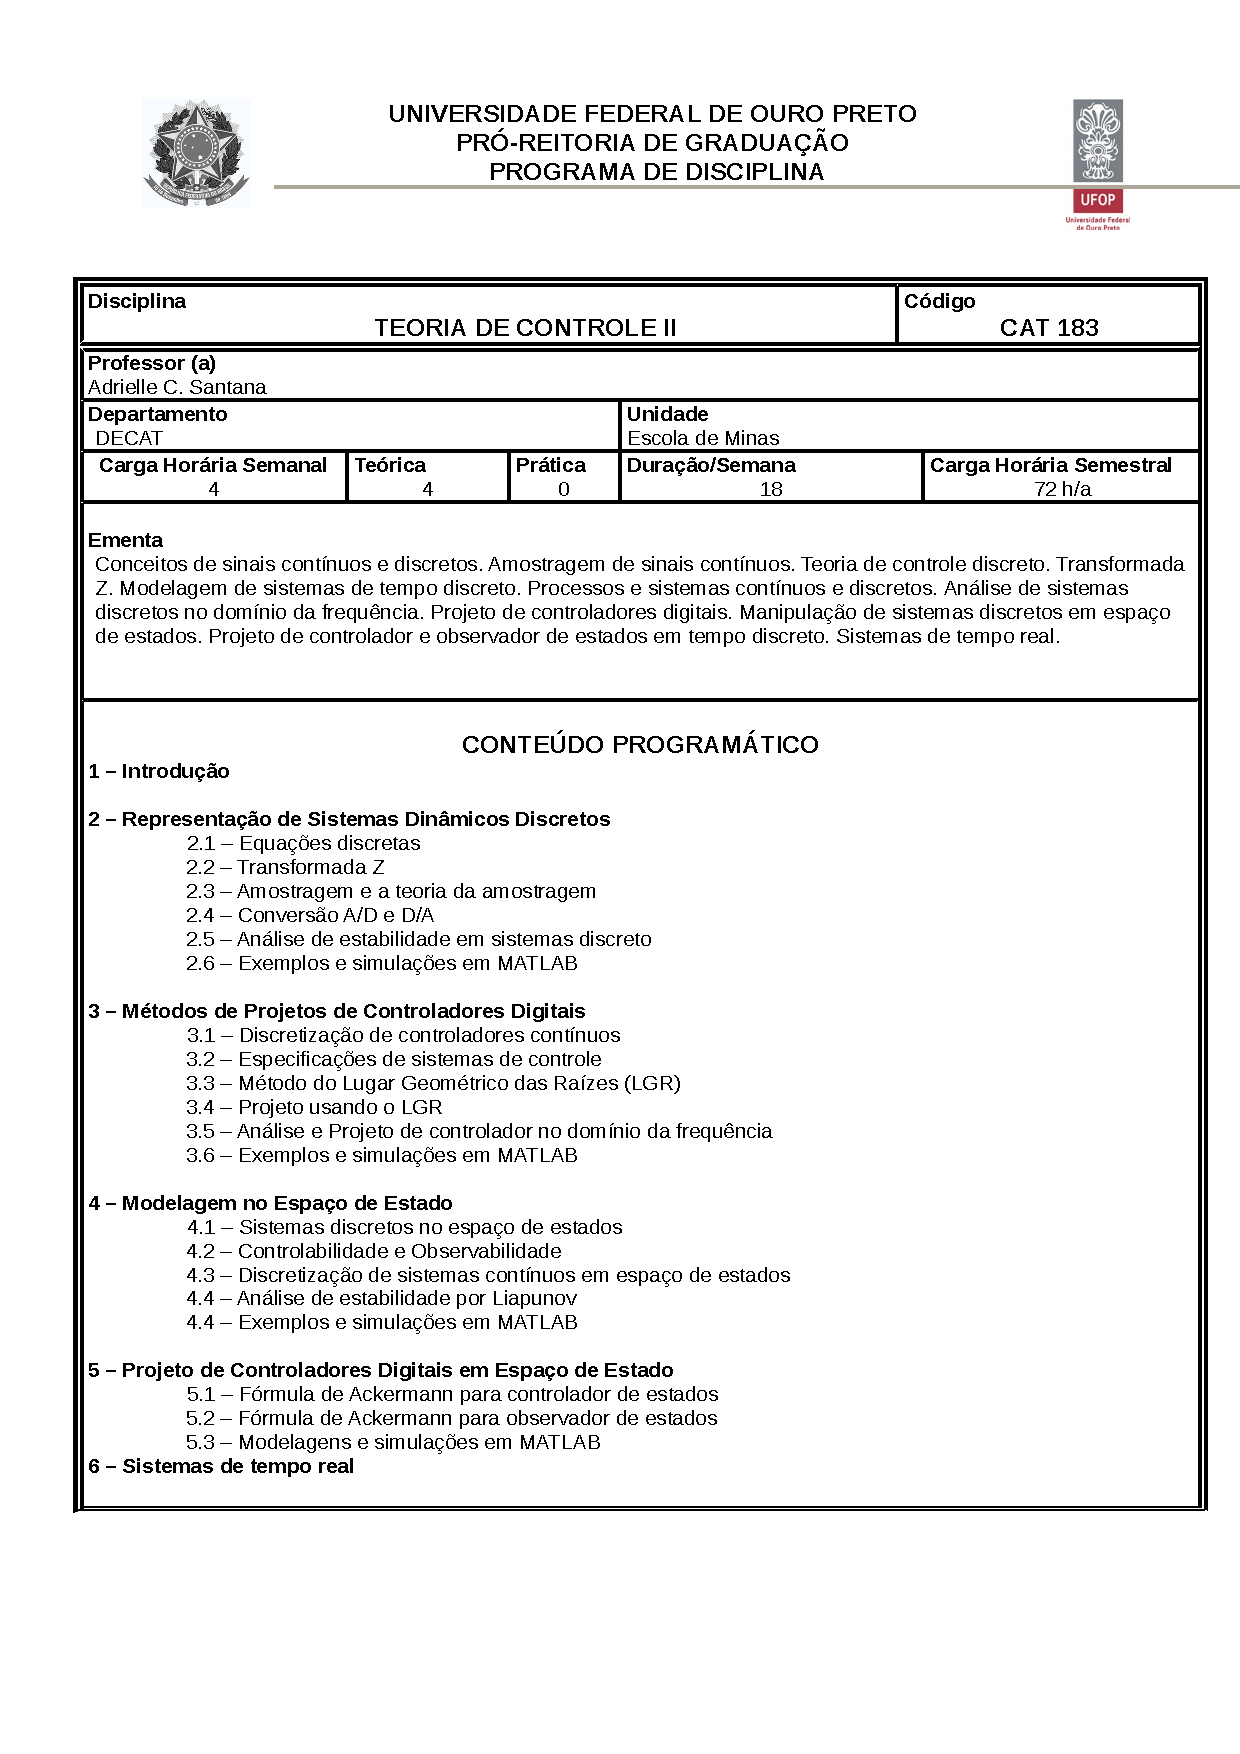
\includegraphics[scale=0.7]{capitulos/anexo1-programas-disciplina/p63.pdf}
	%	\caption{Disciplina do primeiro semestre}
\end{figure}

\begin{figure}[p]
	\centering 
	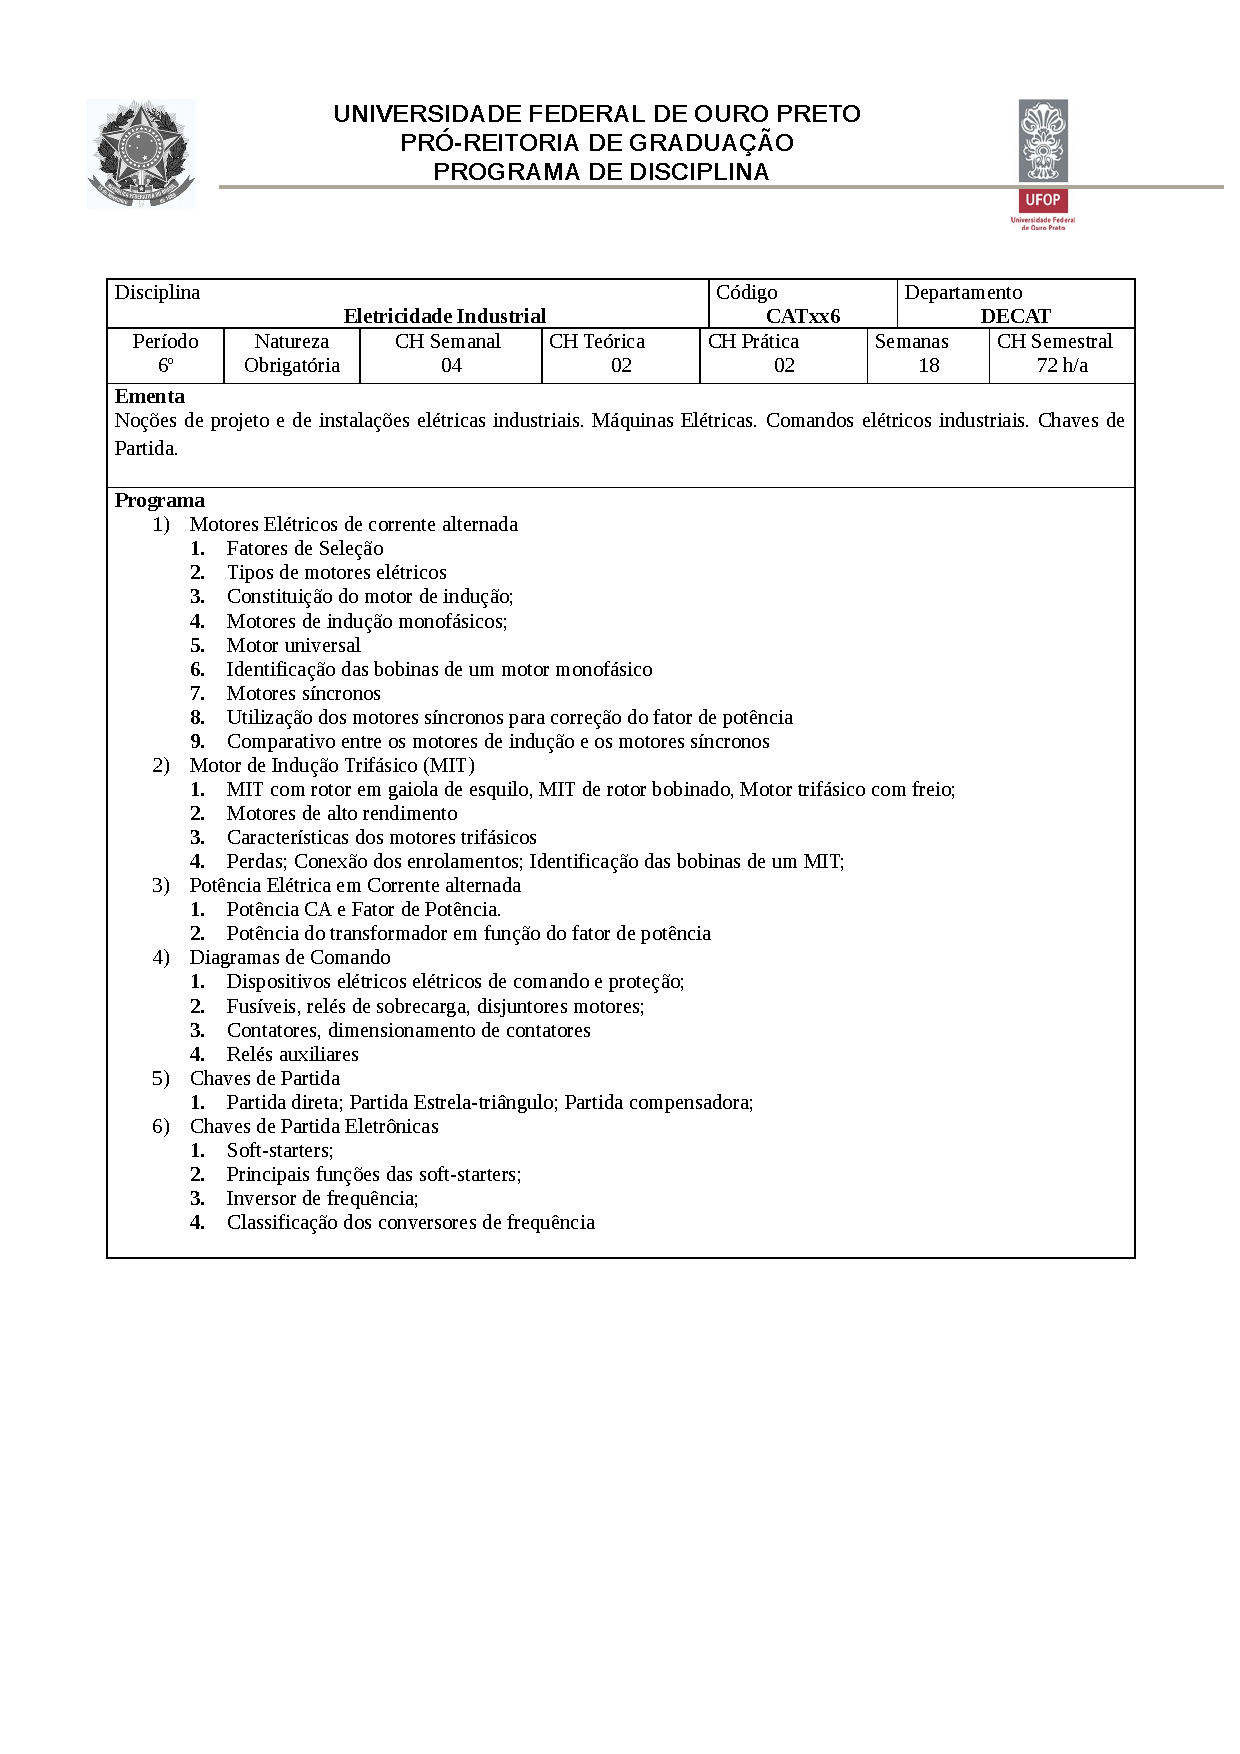
\includegraphics[scale=0.7]{capitulos/anexo1-programas-disciplina/p64.pdf}
	%	\caption{Disciplina do primeiro semestre}
\end{figure}

\begin{figure}[p]
	\centering 
	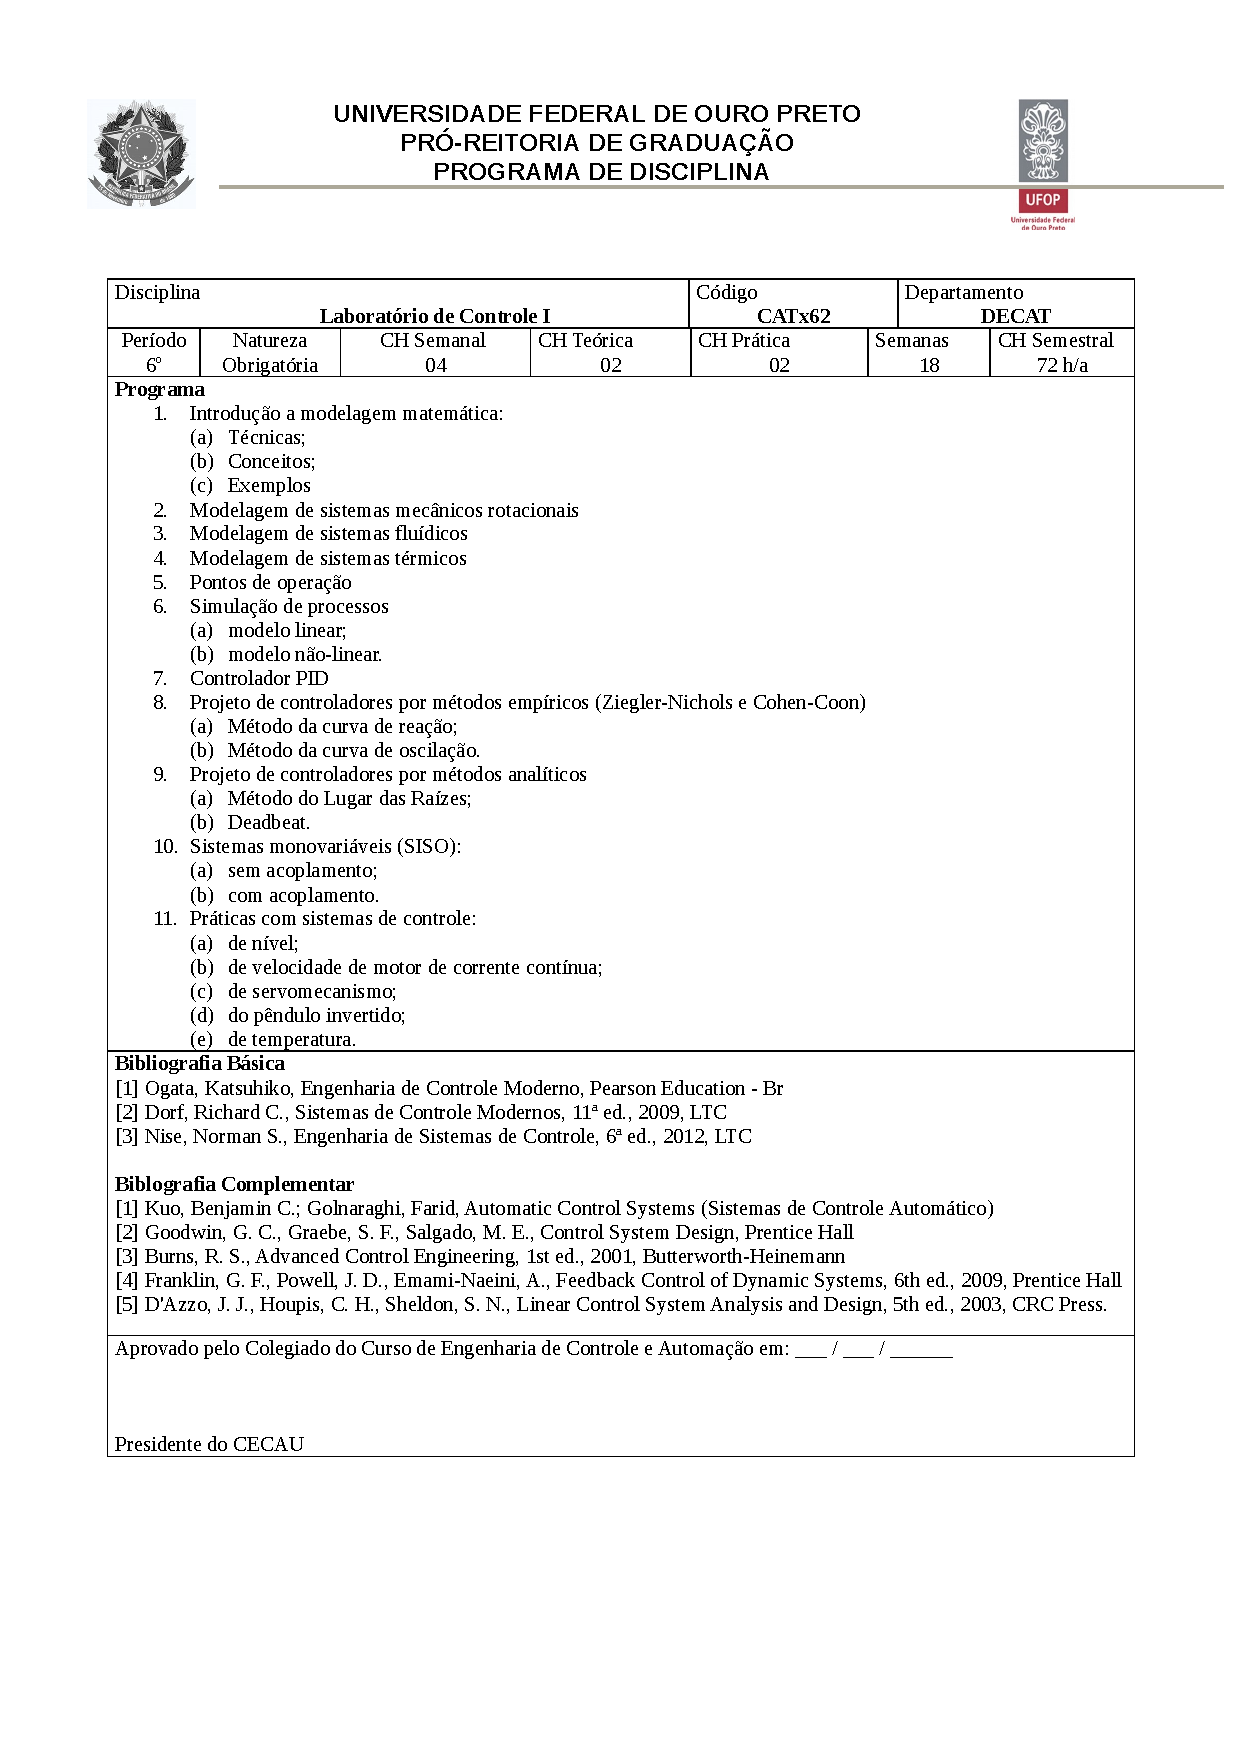
\includegraphics[scale=0.7]{capitulos/anexo1-programas-disciplina/p65.pdf}
	%	\caption{Disciplina do primeiro semestre}
\end{figure}

%setimo semestre
\begin{figure}[p]
	\centering 
	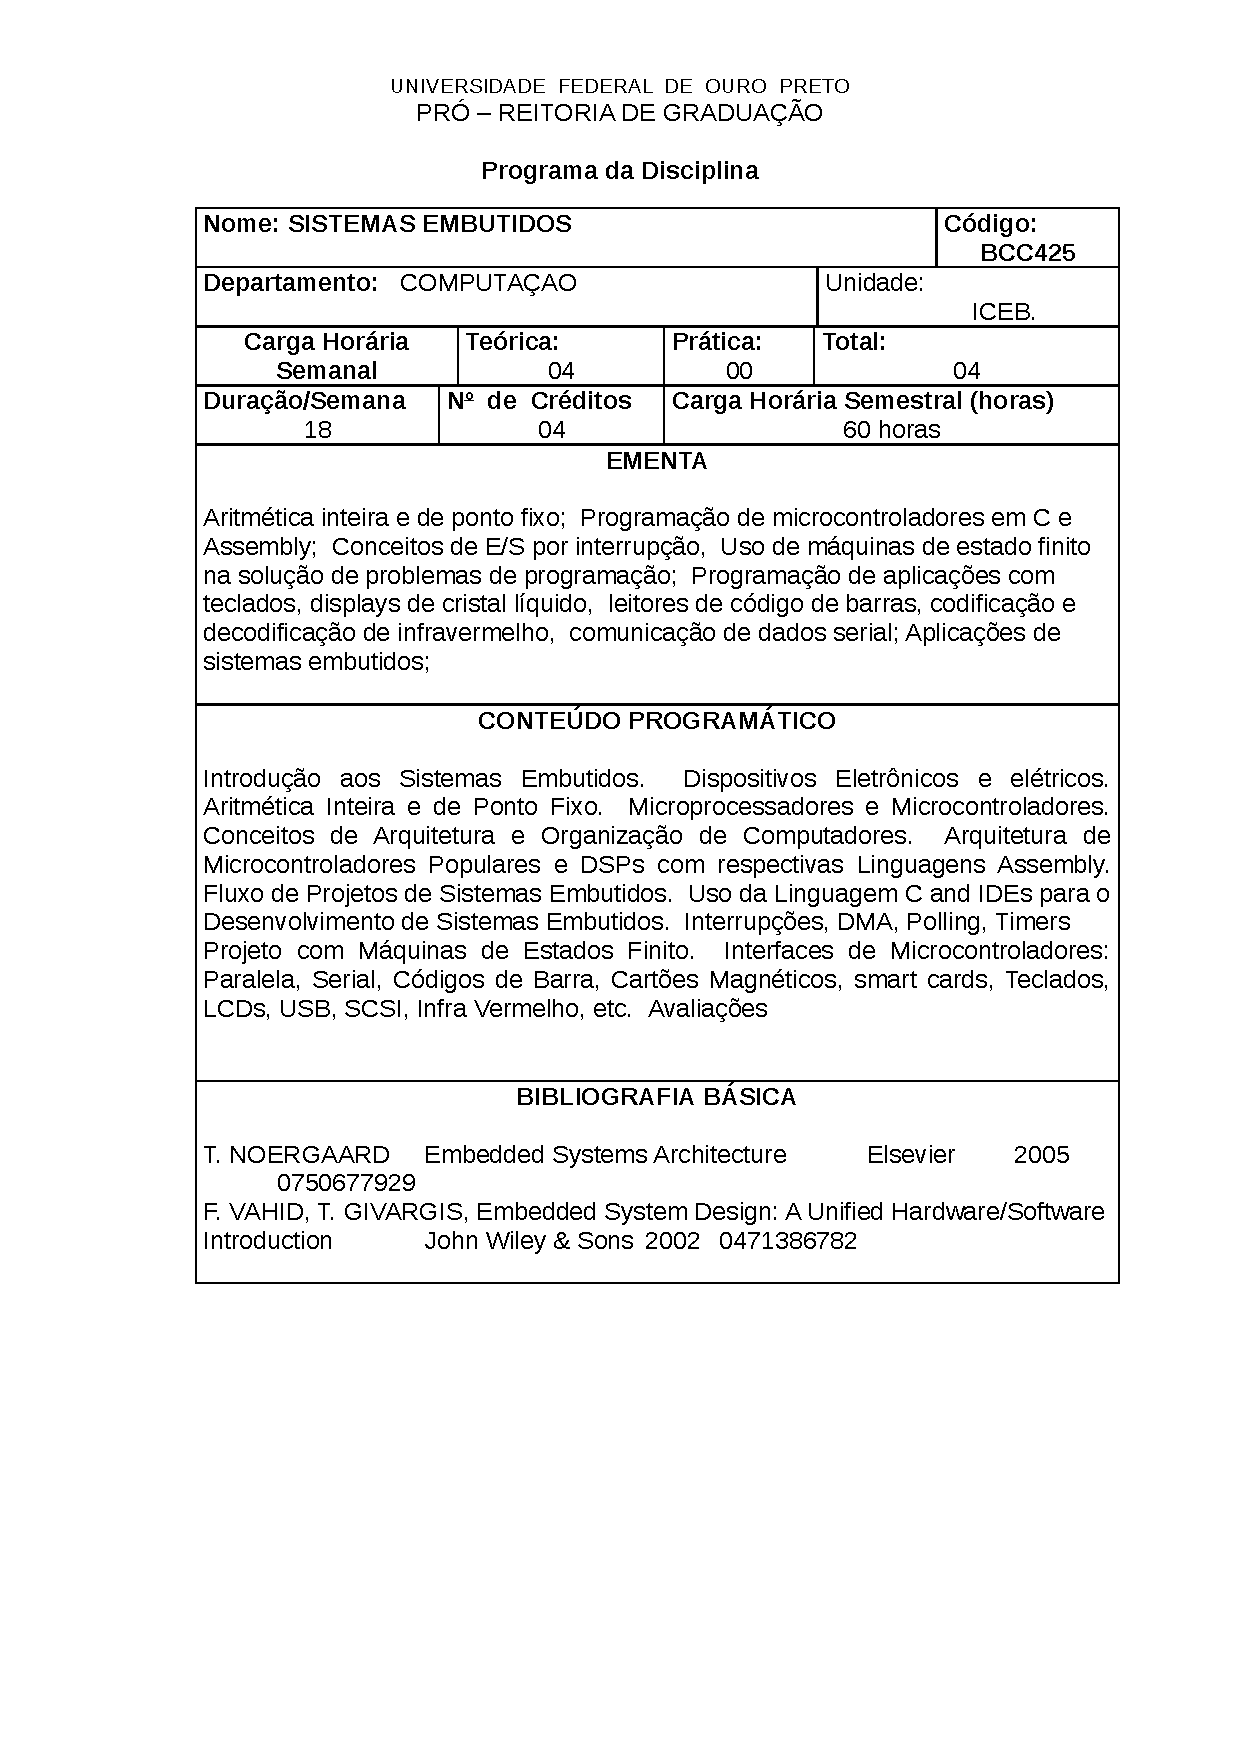
\includegraphics[scale=0.7]{capitulos/anexo1-programas-disciplina/p71.pdf}
	%	\caption{Disciplina do primeiro semestre}
\end{figure}

\begin{figure}[p]
	\centering 
	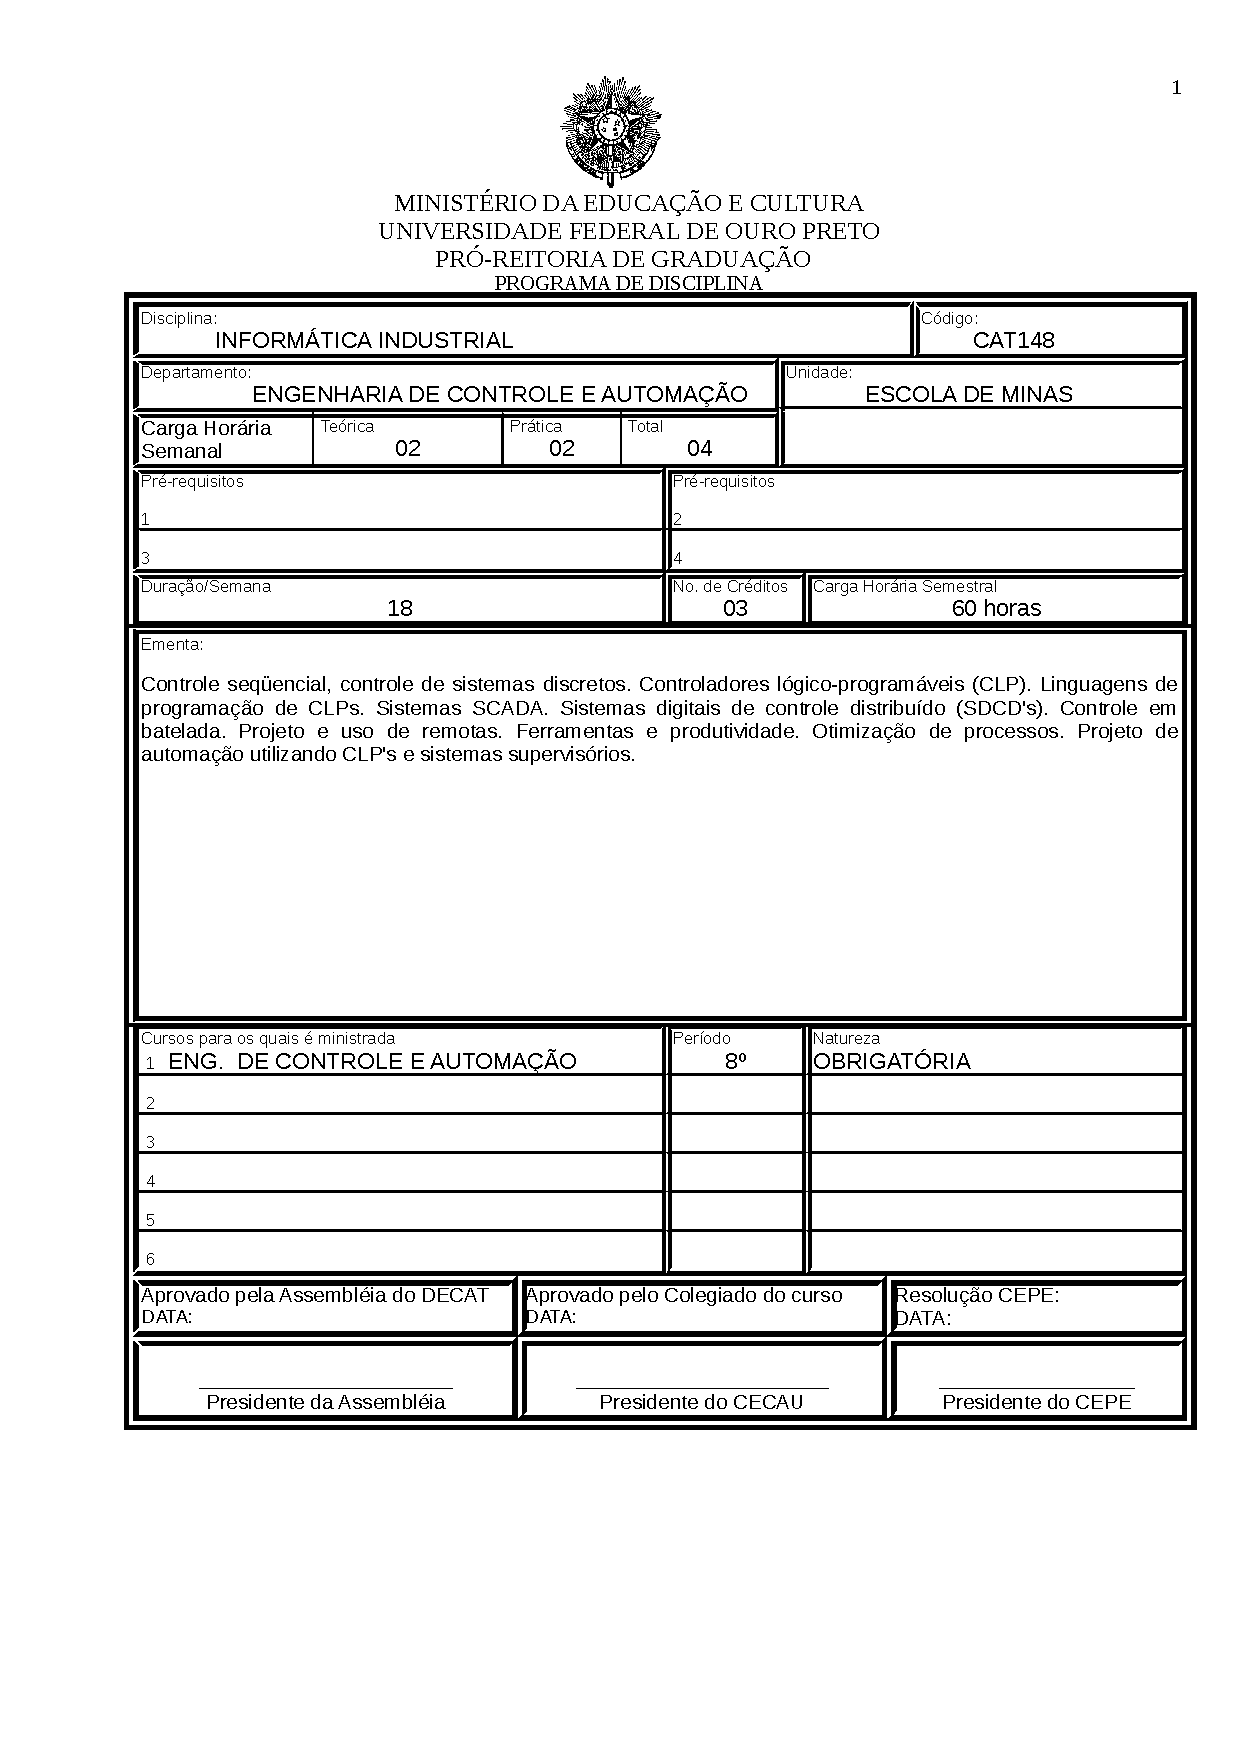
\includegraphics[scale=0.7]{capitulos/anexo1-programas-disciplina/p72.pdf}
	%	\caption{Disciplina do primeiro semestre}
\end{figure}

\begin{figure}[p]
	\centering 
	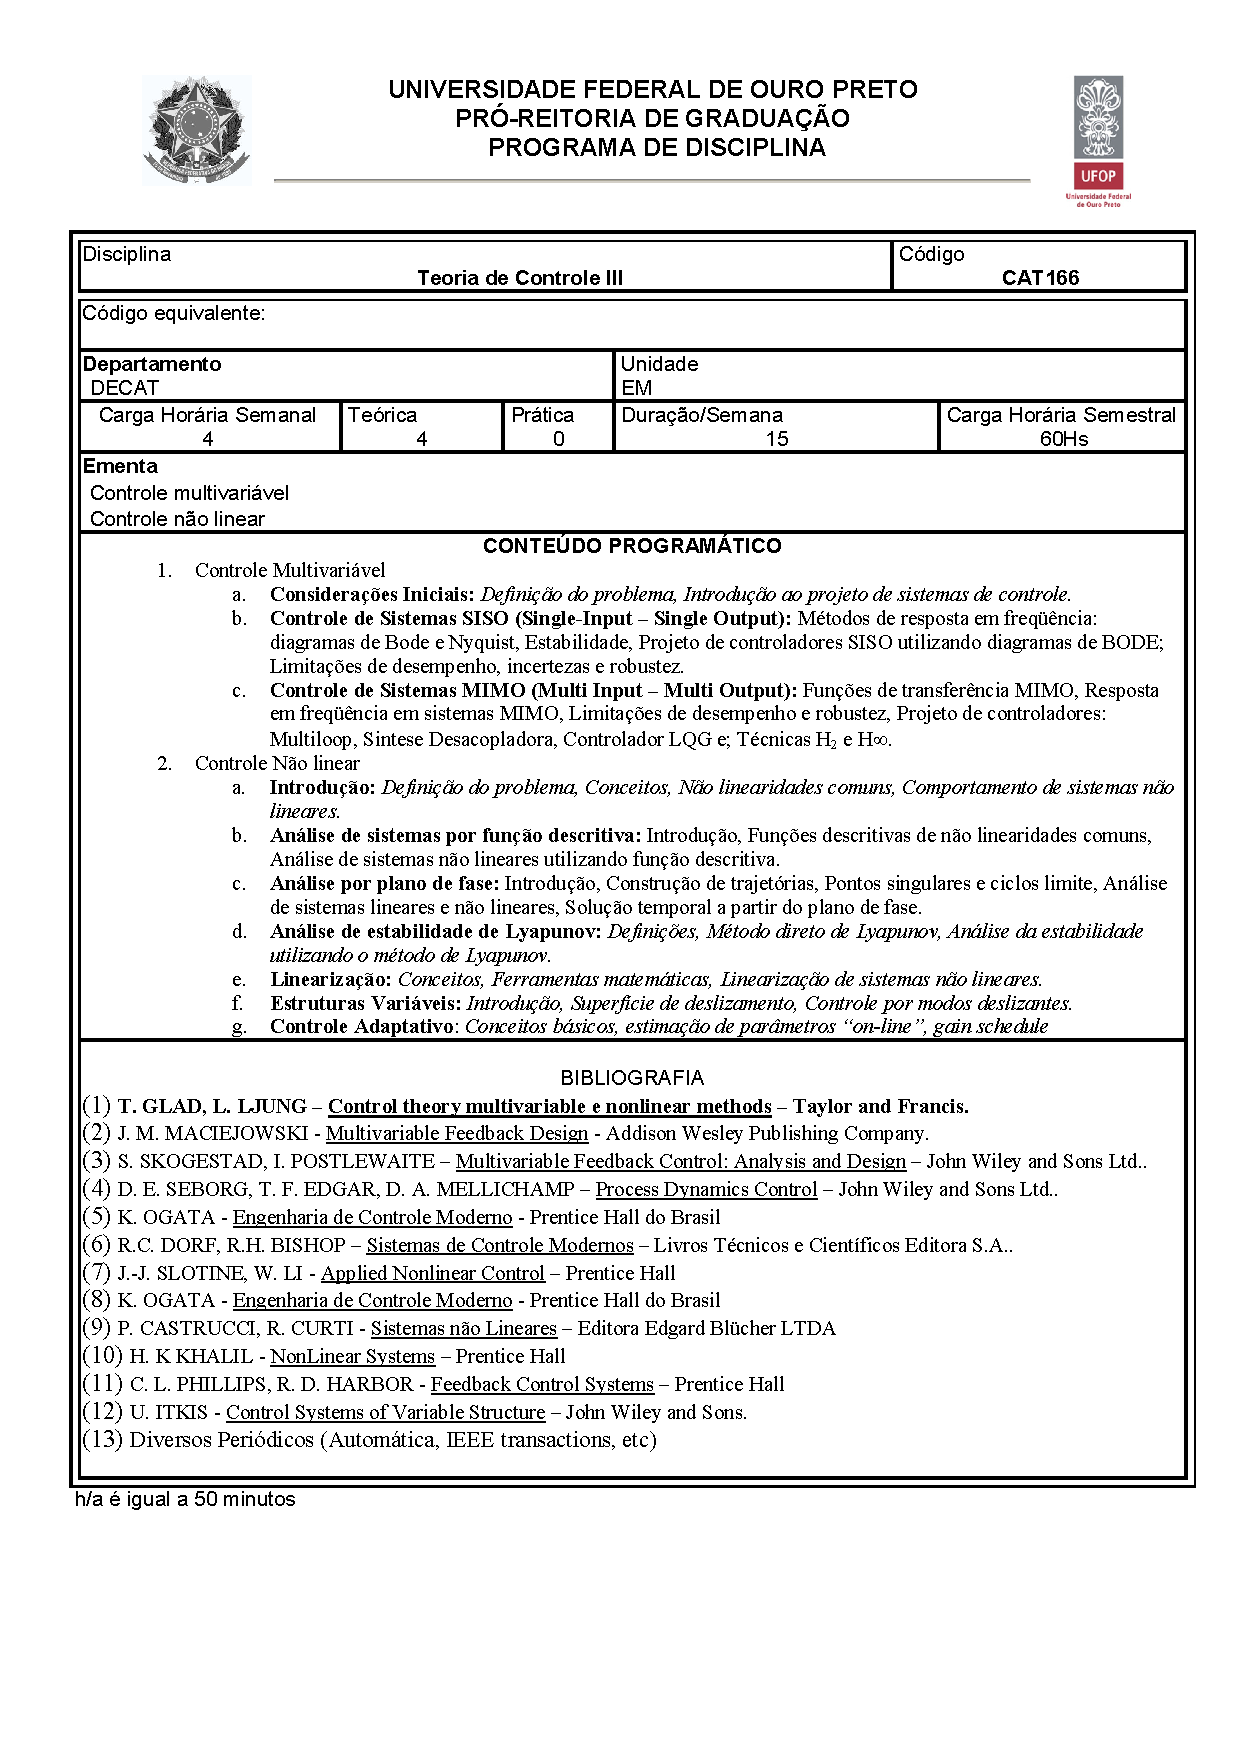
\includegraphics[scale=0.7]{capitulos/anexo1-programas-disciplina/p73.pdf}
	%	\caption{Disciplina do primeiro semestre}
\end{figure}

\begin{figure}[p]
	\centering 
	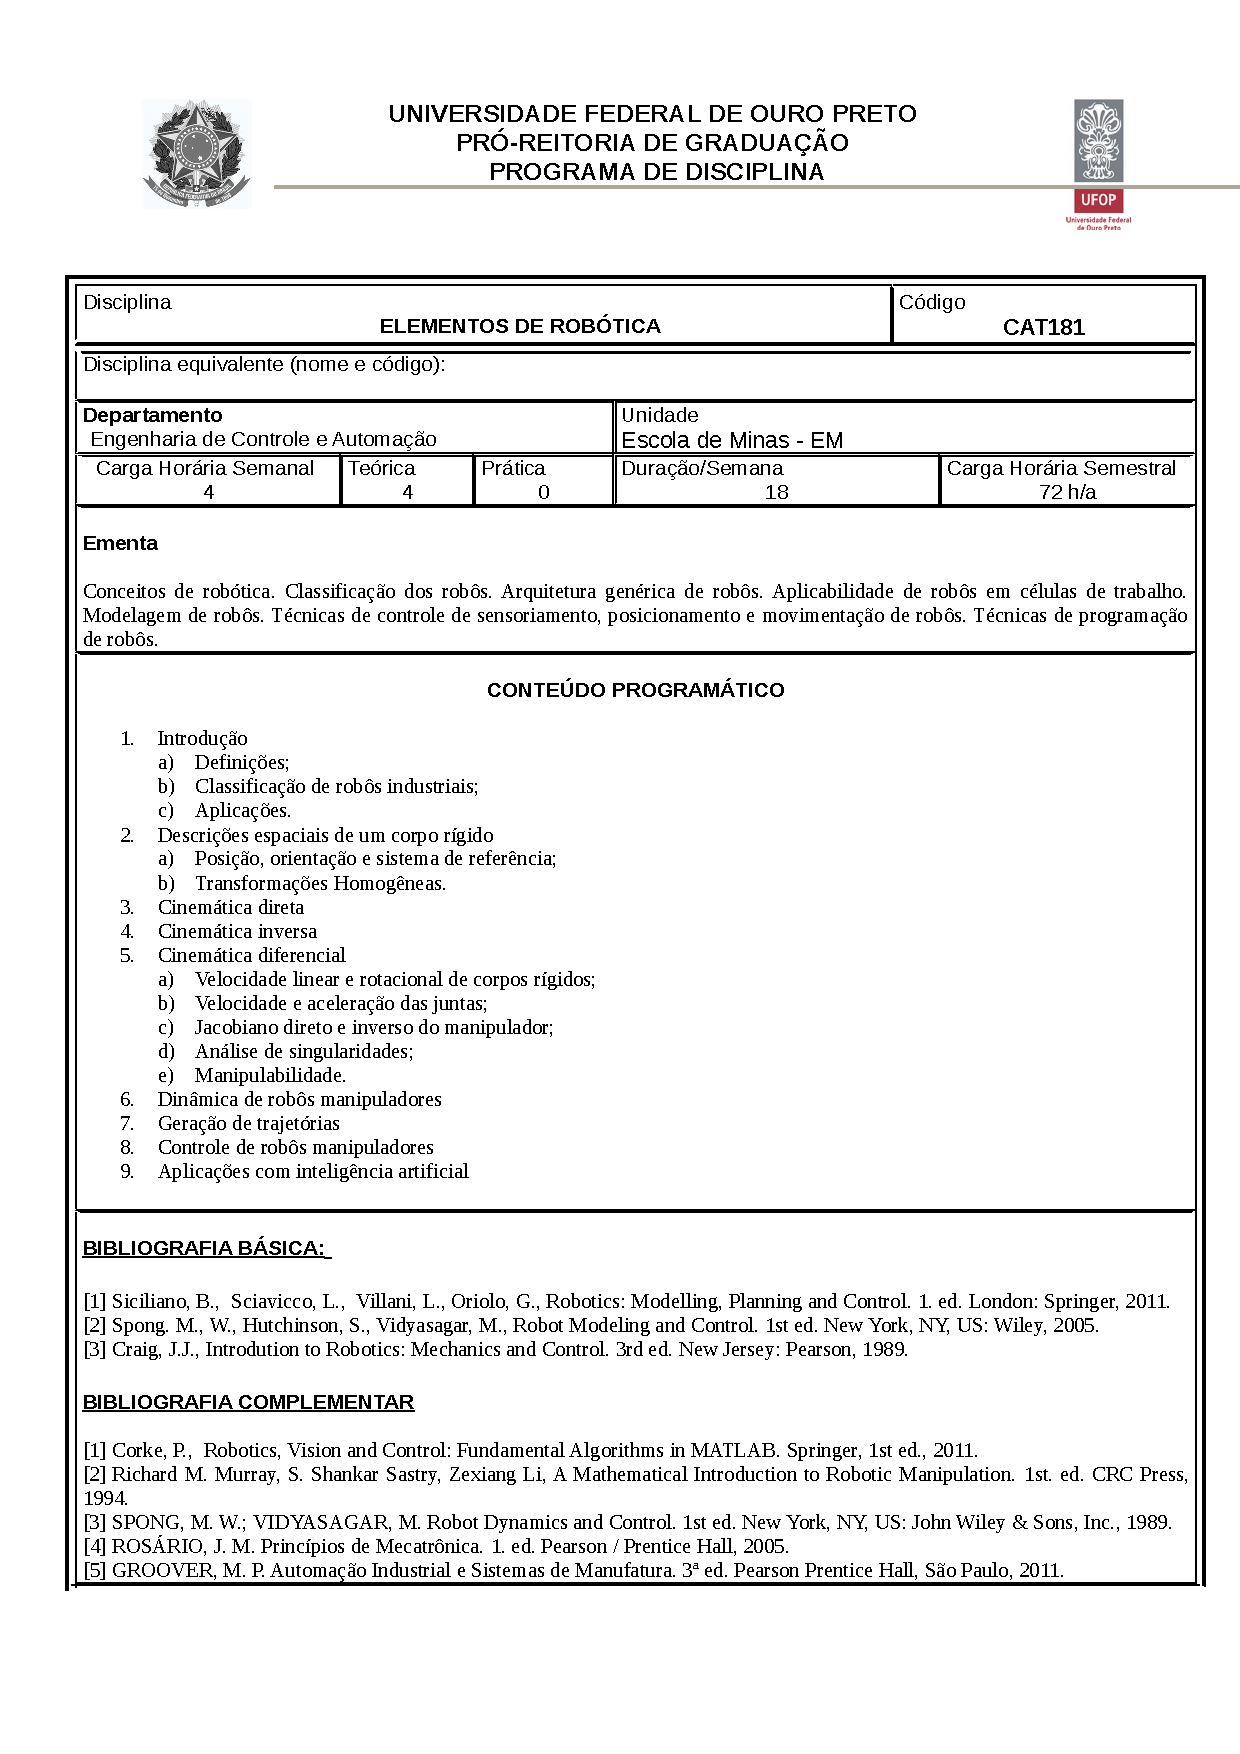
\includegraphics[scale=0.7]{capitulos/anexo1-programas-disciplina/p74.pdf}
	%	\caption{Disciplina do primeiro semestre}
\end{figure}

%Oitavo semestre
\begin{figure}[p]
	\centering 
	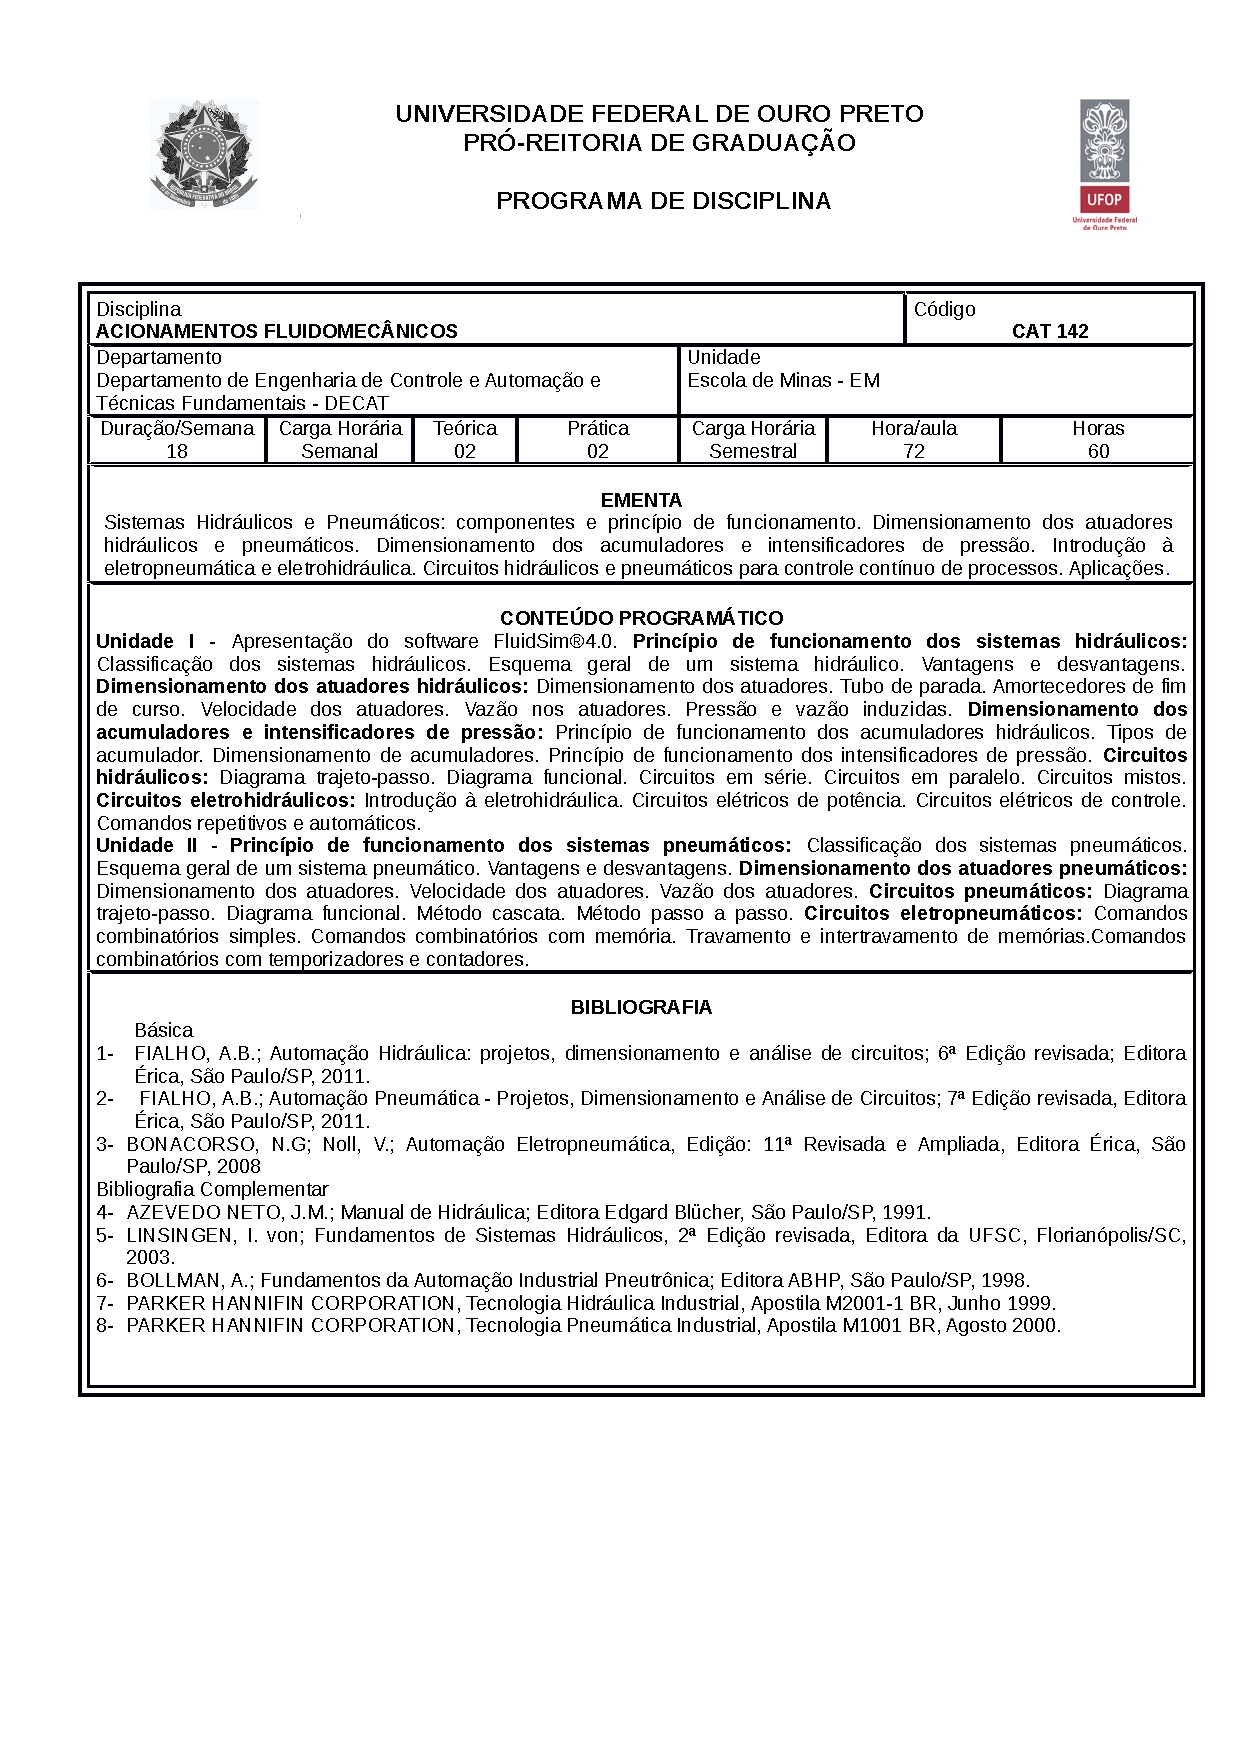
\includegraphics[scale=0.7]{capitulos/anexo1-programas-disciplina/p81.pdf}
	%	\caption{Disciplina do primeiro semestre}
\end{figure}

\begin{figure}[p]
	\centering 
	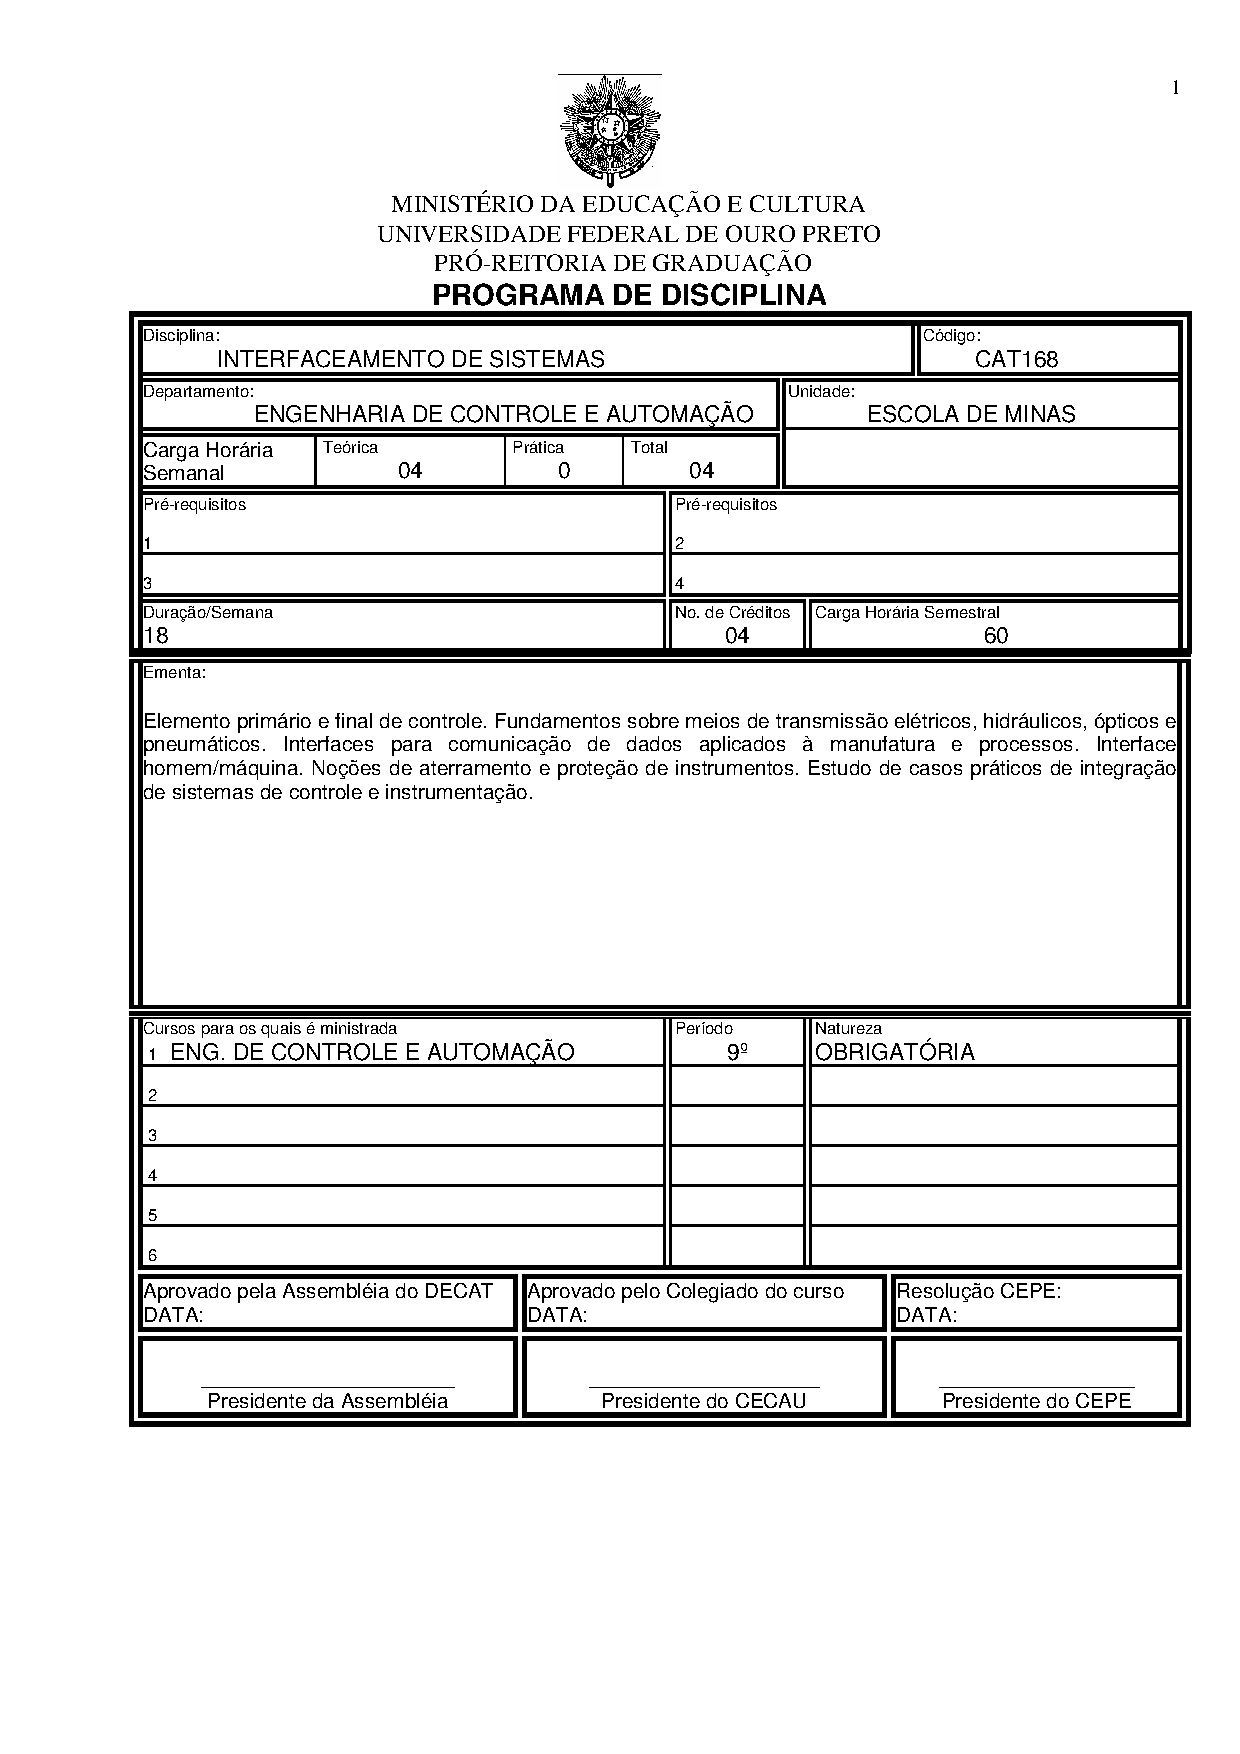
\includegraphics[scale=0.7]{capitulos/anexo1-programas-disciplina/p82.pdf}
	%	\caption{Disciplina do primeiro semestre}
\end{figure}

\begin{figure}[p]
	\centering 
	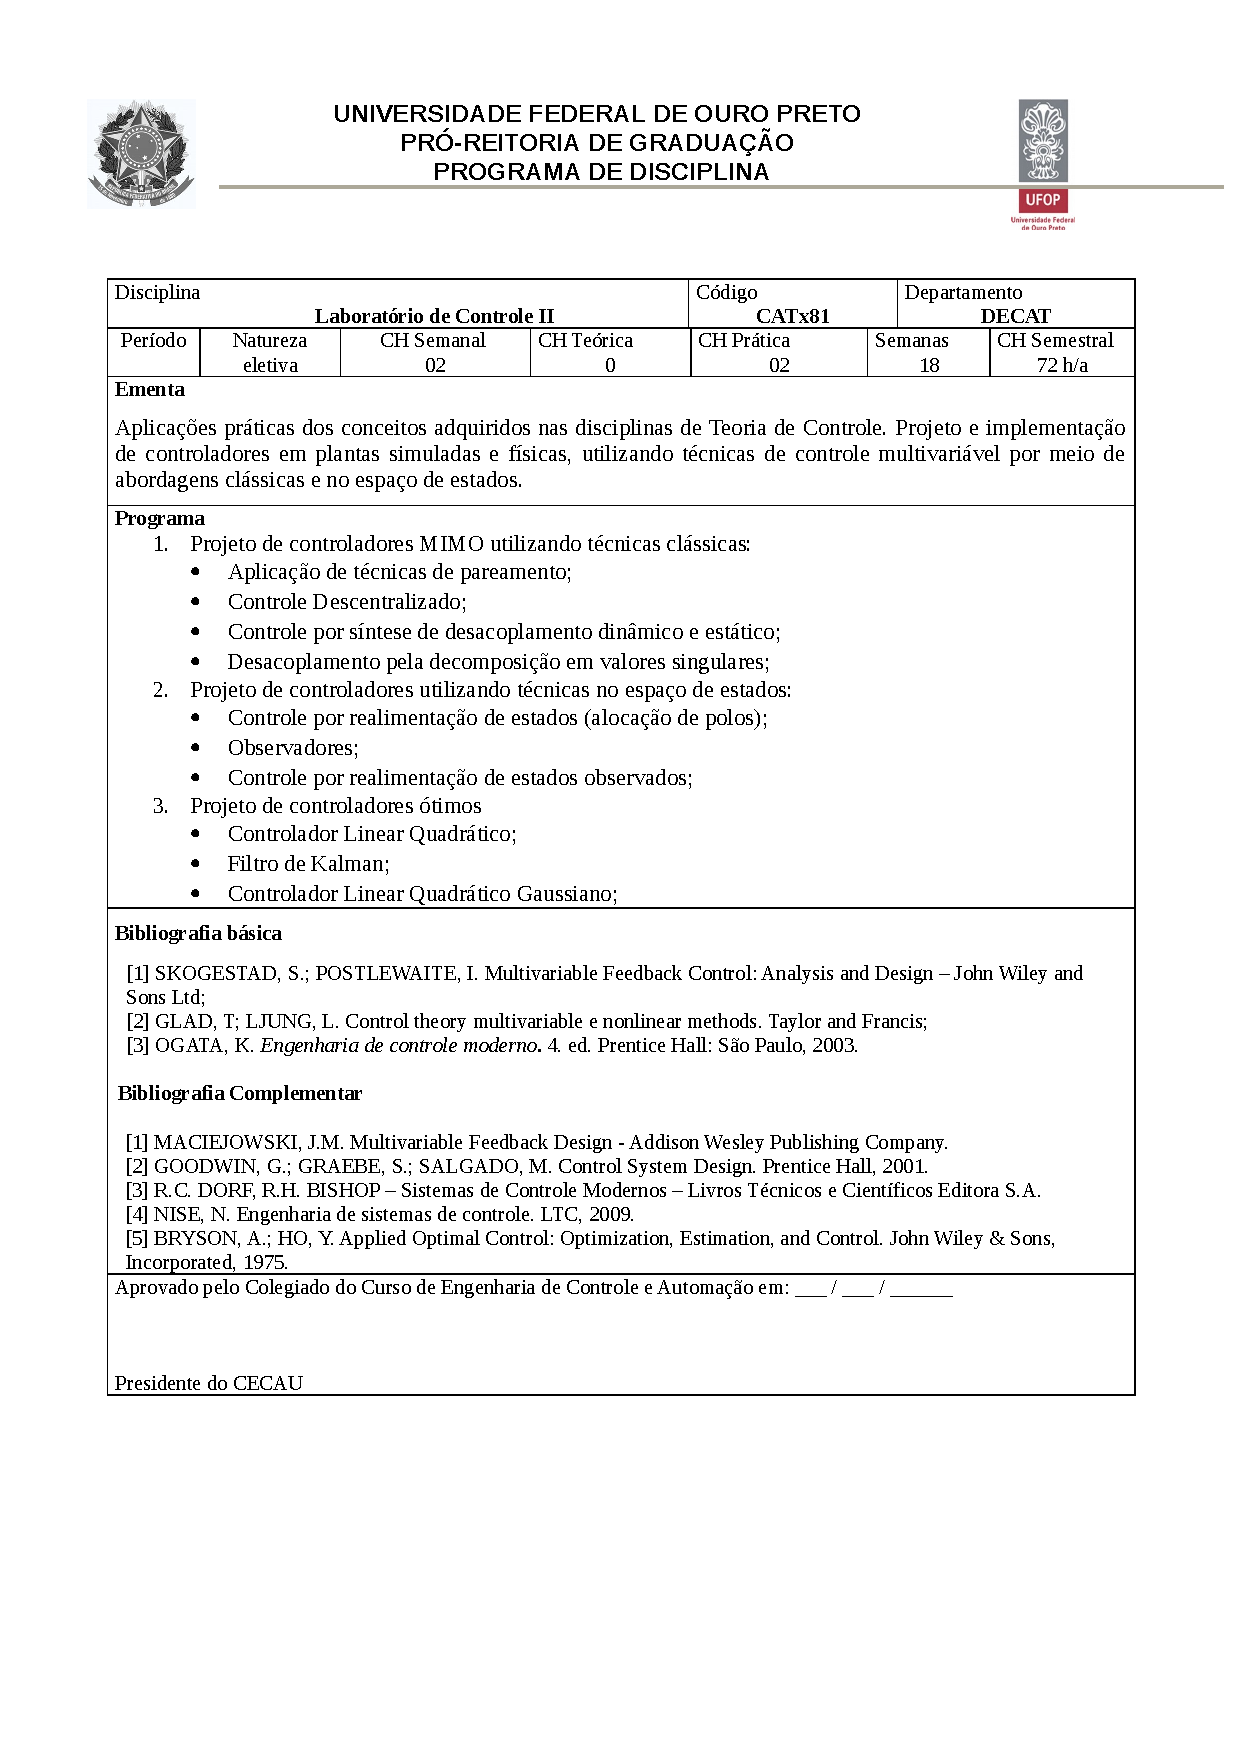
\includegraphics[scale=0.7]{capitulos/anexo1-programas-disciplina/p83.pdf}
	%	\caption{Disciplina do primeiro semestre}
\end{figure}

\begin{figure}[p]
	\centering 
	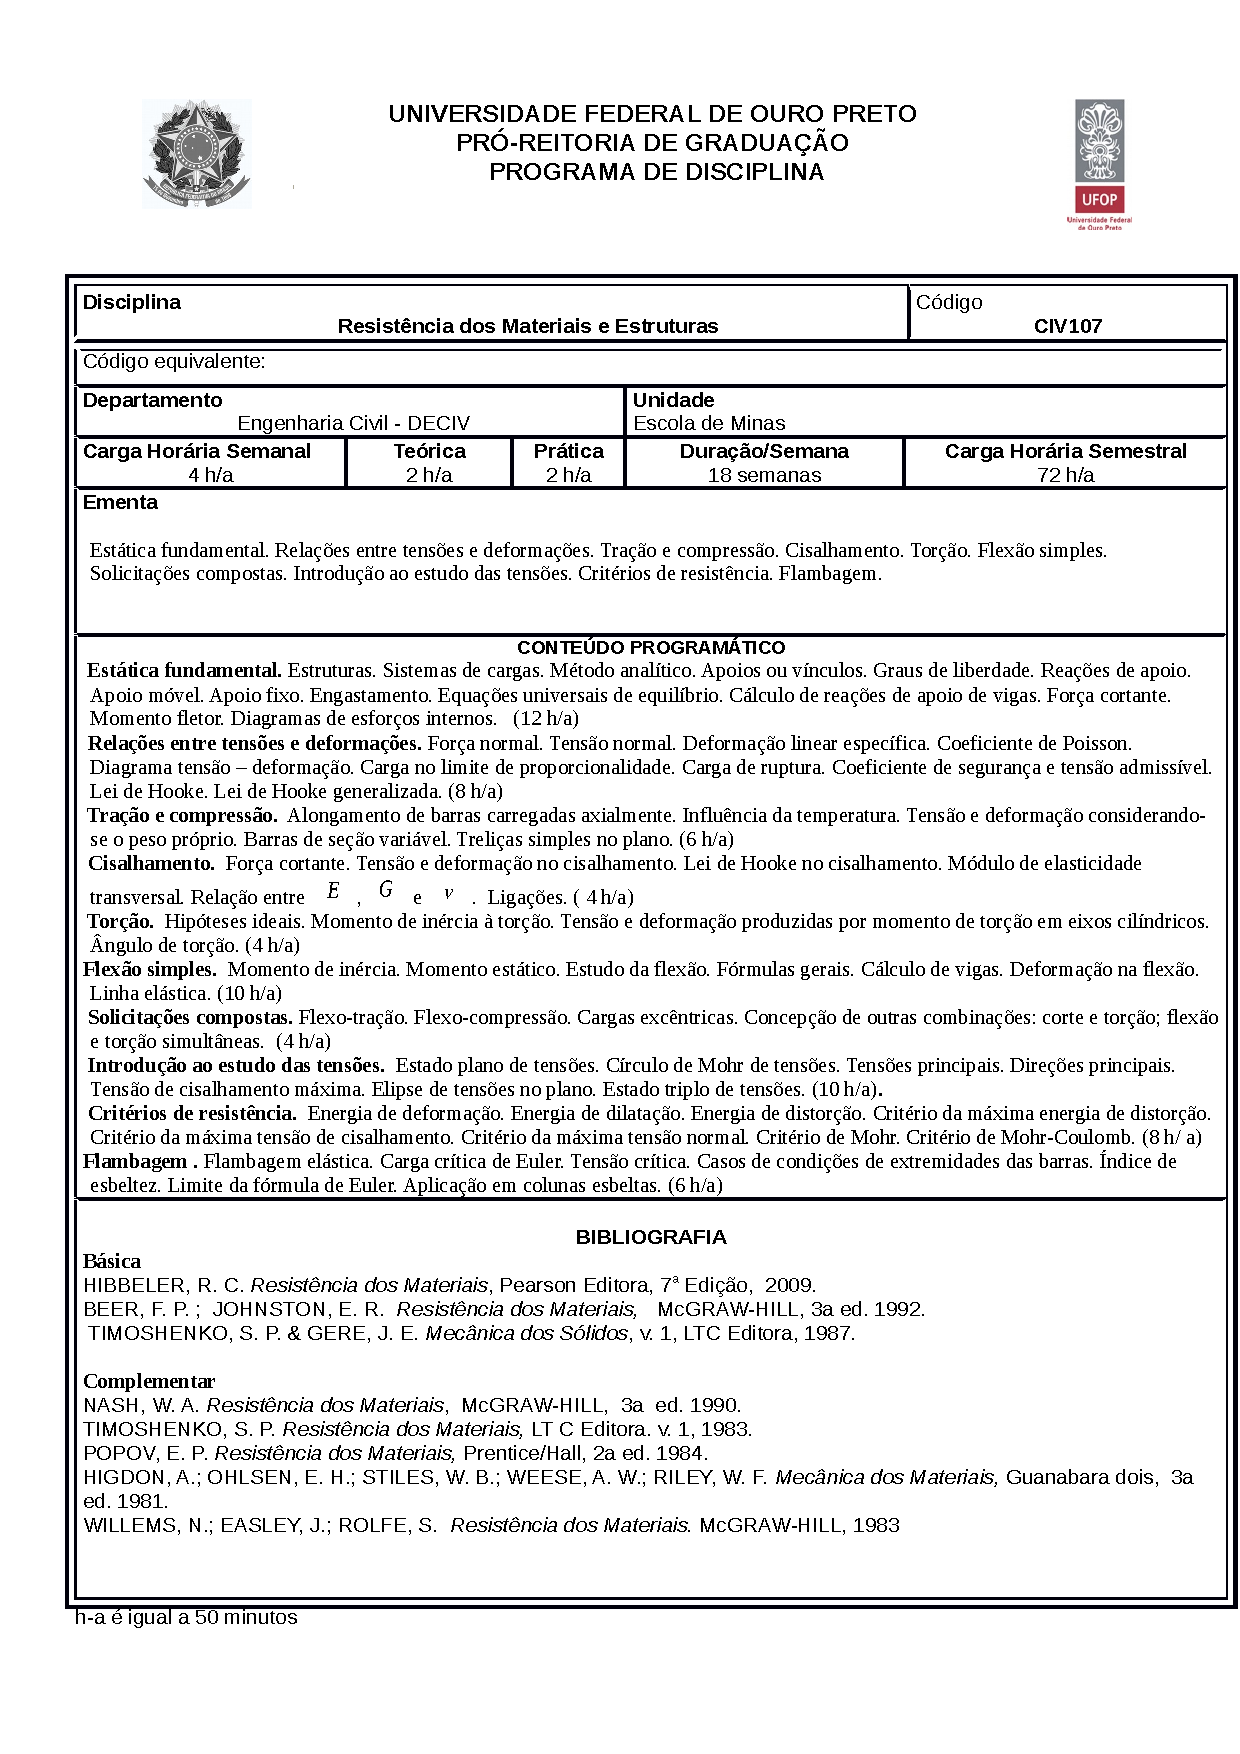
\includegraphics[scale=0.7]{capitulos/anexo1-programas-disciplina/p84.pdf}
	%	\caption{Disciplina do primeiro semestre}
\end{figure}

%Nono semestre
\begin{figure}[p]
	\centering 
	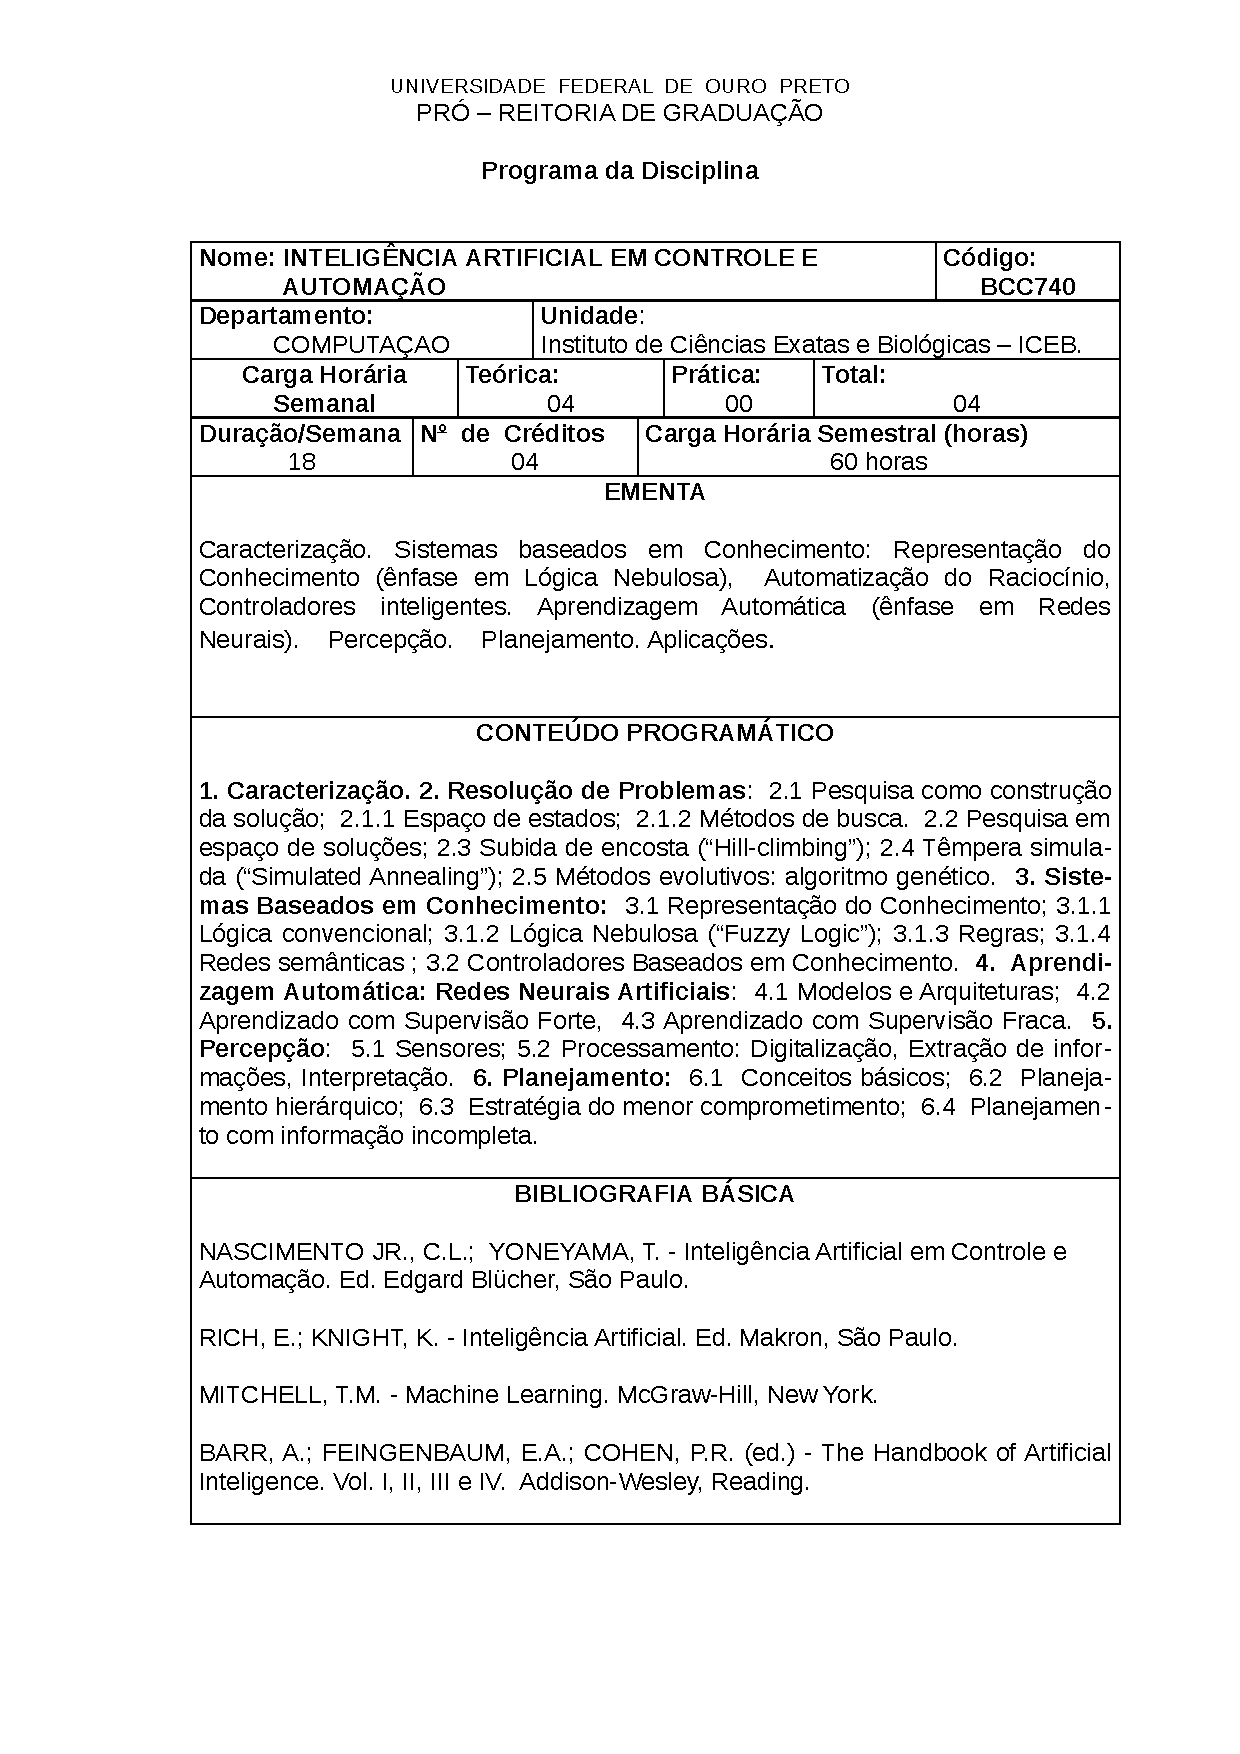
\includegraphics[scale=0.7]{capitulos/anexo1-programas-disciplina/p91.pdf}
	%	\caption{Disciplina do primeiro semestre}
\end{figure}

\begin{figure}[p]
	\centering 
	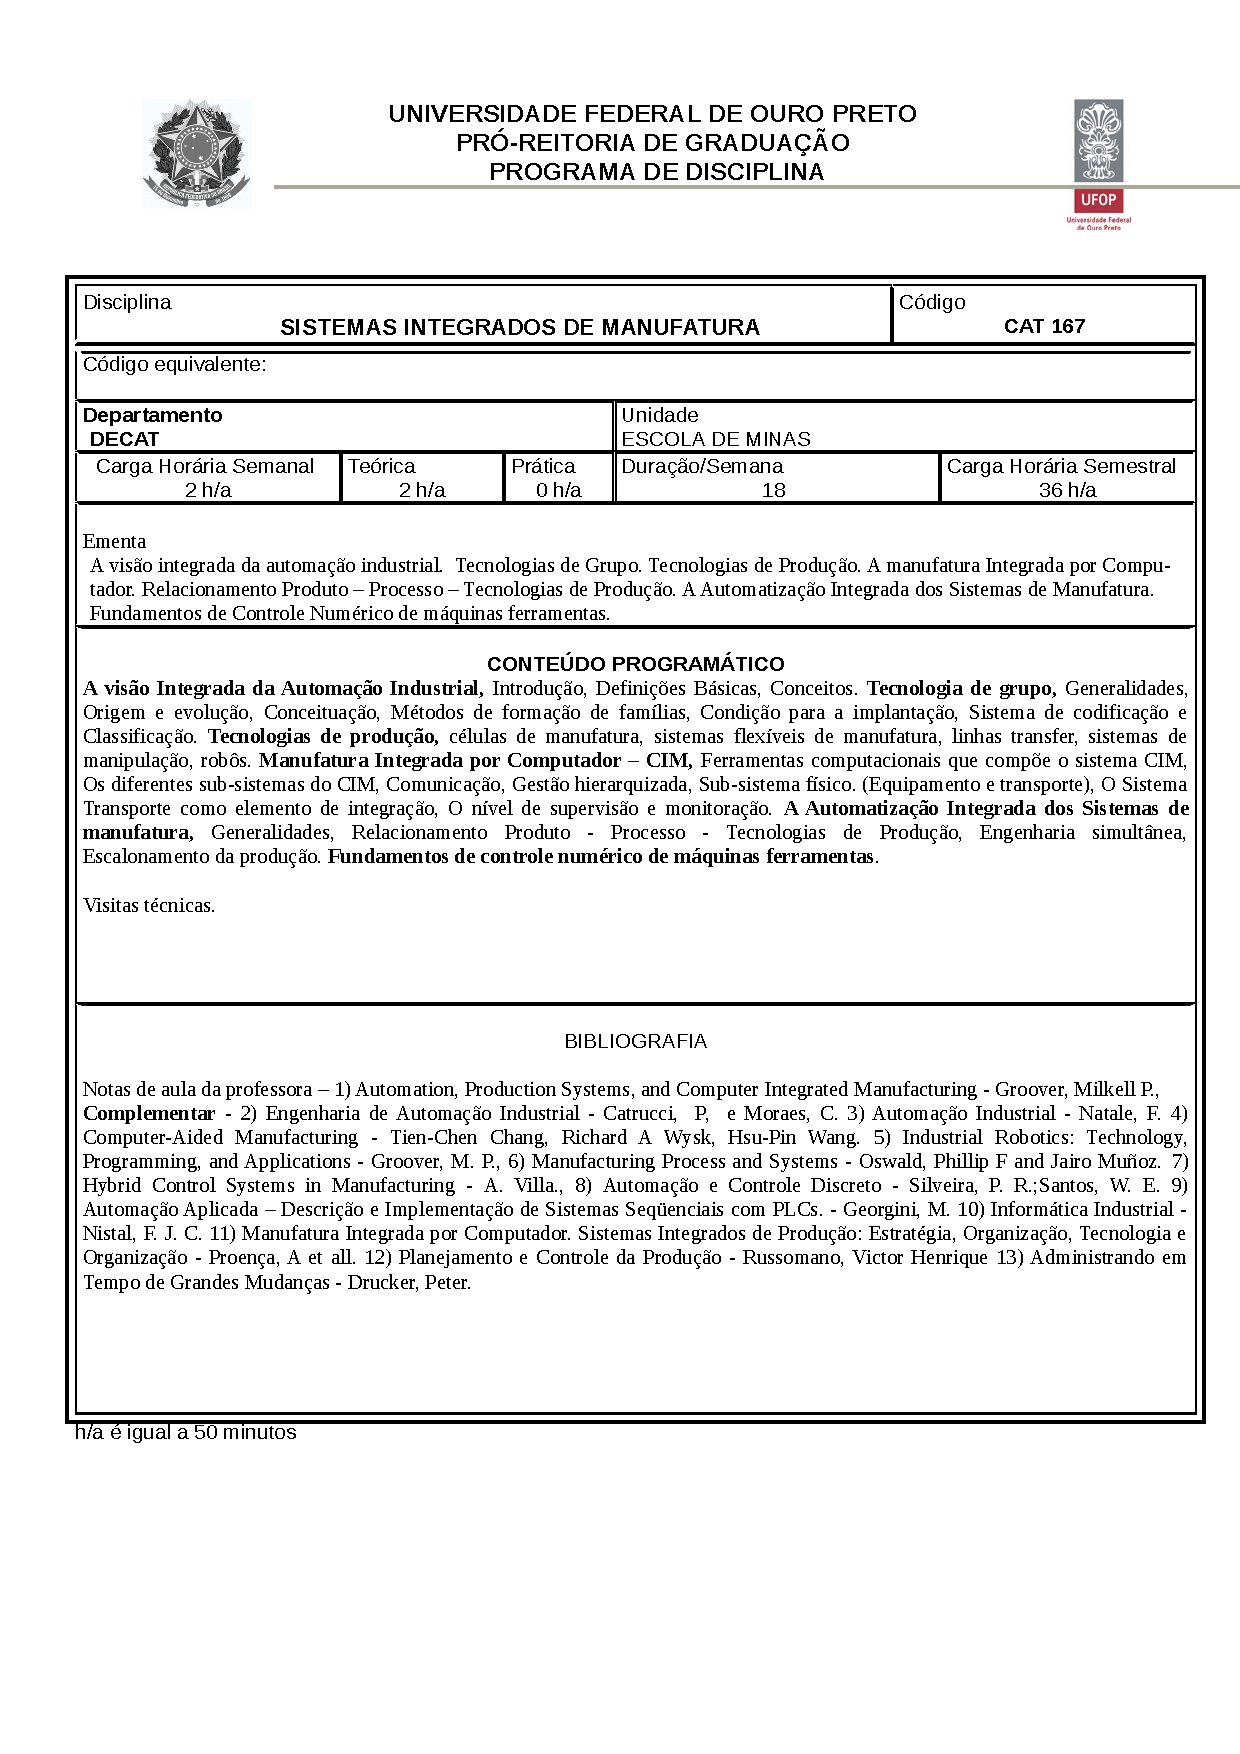
\includegraphics[scale=0.7]{capitulos/anexo1-programas-disciplina/p92.pdf}
	%	\caption{Disciplina do primeiro semestre}
\end{figure}

\begin{figure}[p]
	\centering 
	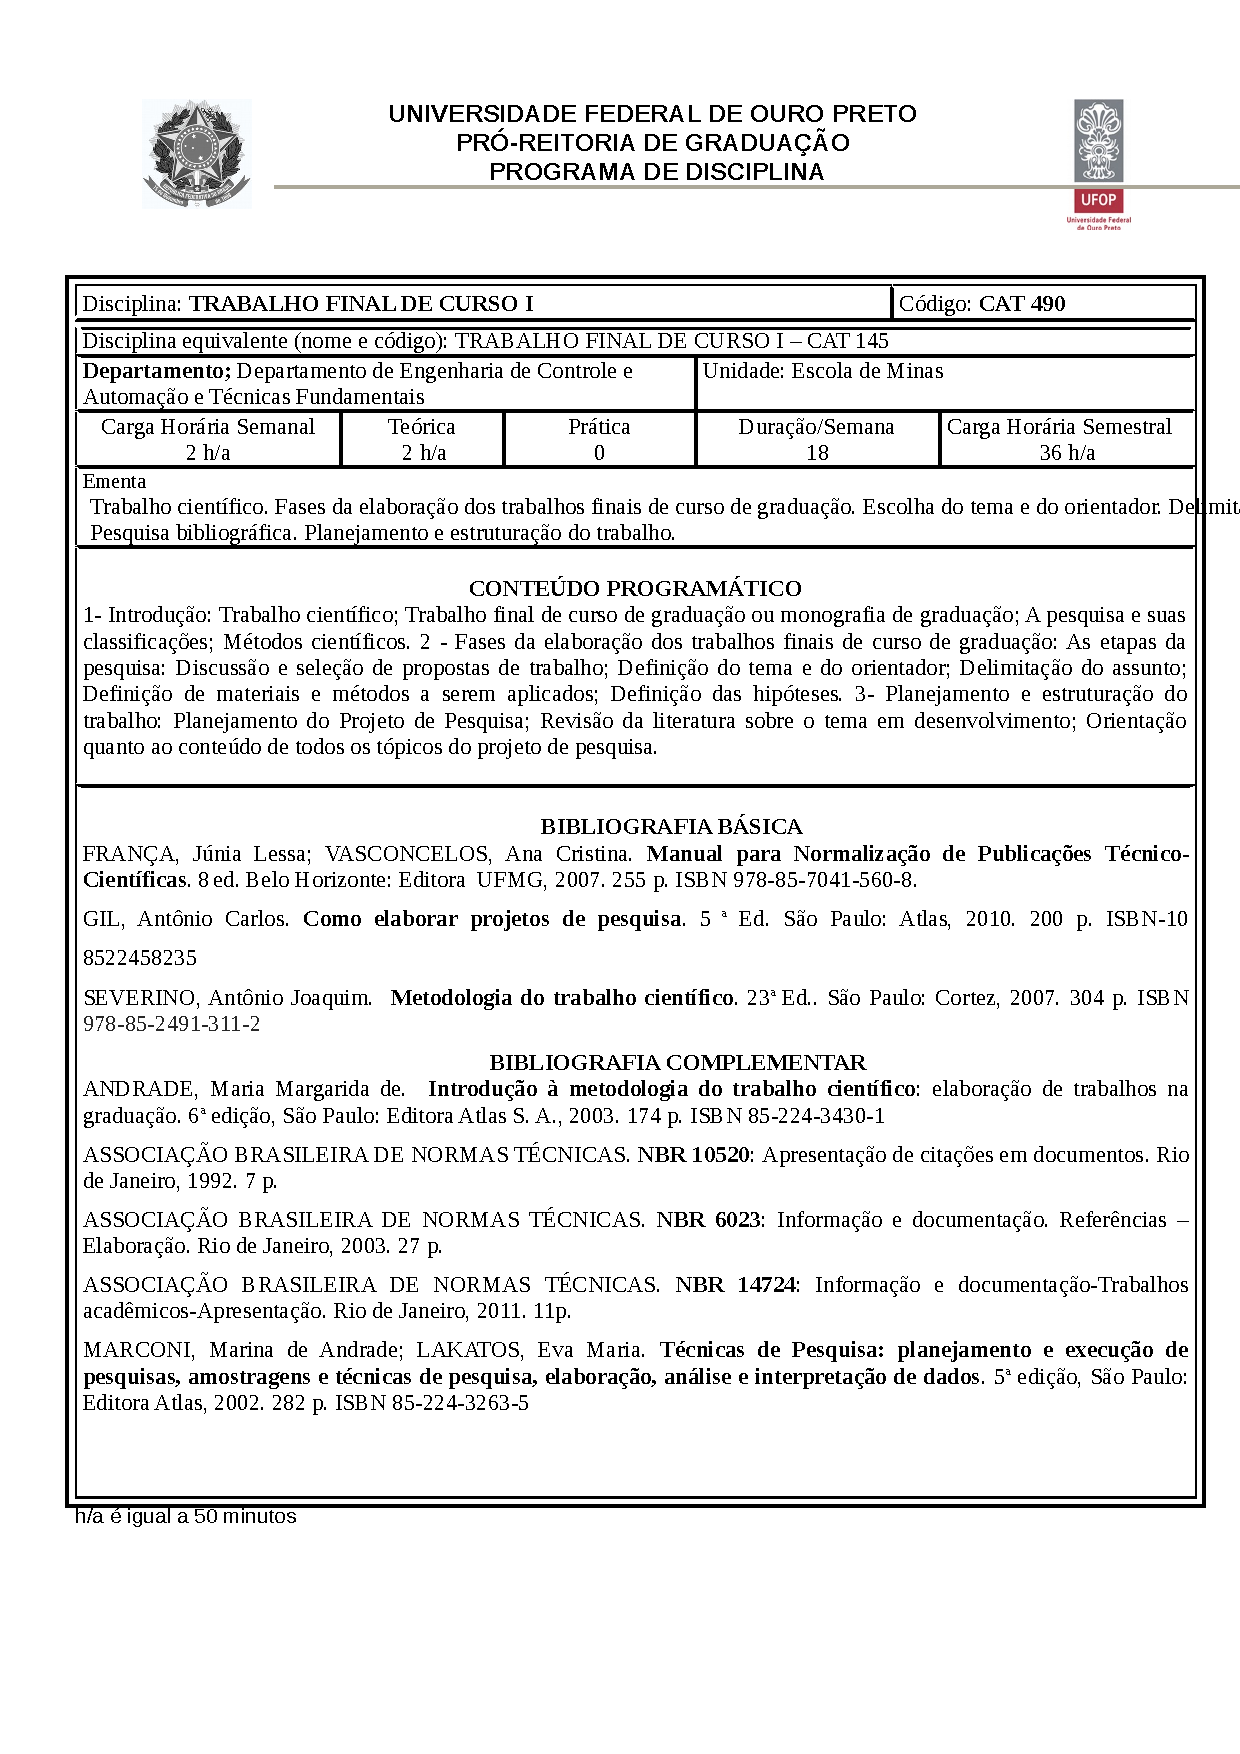
\includegraphics[scale=0.7]{capitulos/anexo1-programas-disciplina/p93.pdf}
	%	\caption{Disciplina do primeiro semestre}
\end{figure}

\begin{figure}[p]
	\centering 
	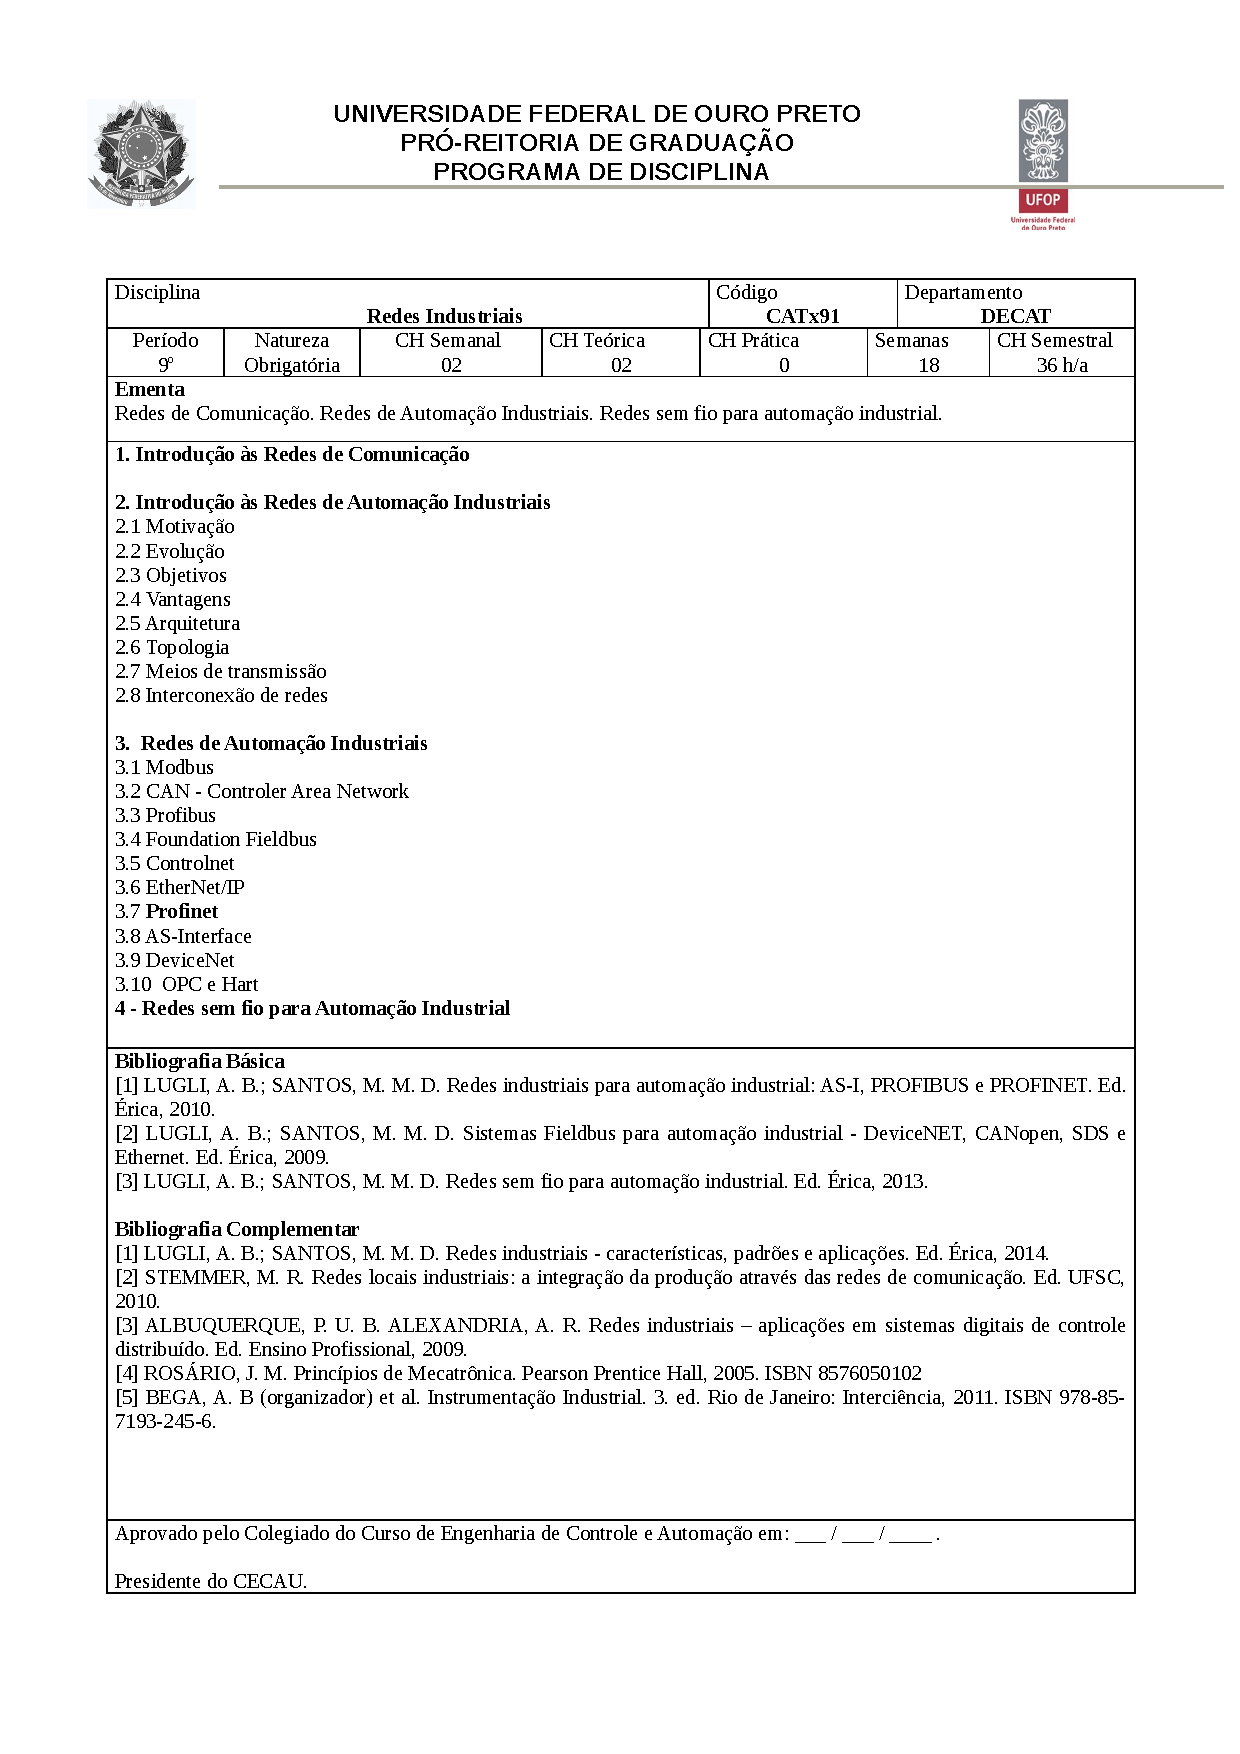
\includegraphics[scale=0.7]{capitulos/anexo1-programas-disciplina/p94.pdf}
	%	\caption{Disciplina do primeiro semestre}
\end{figure}

\begin{figure}[p]
	\centering 
	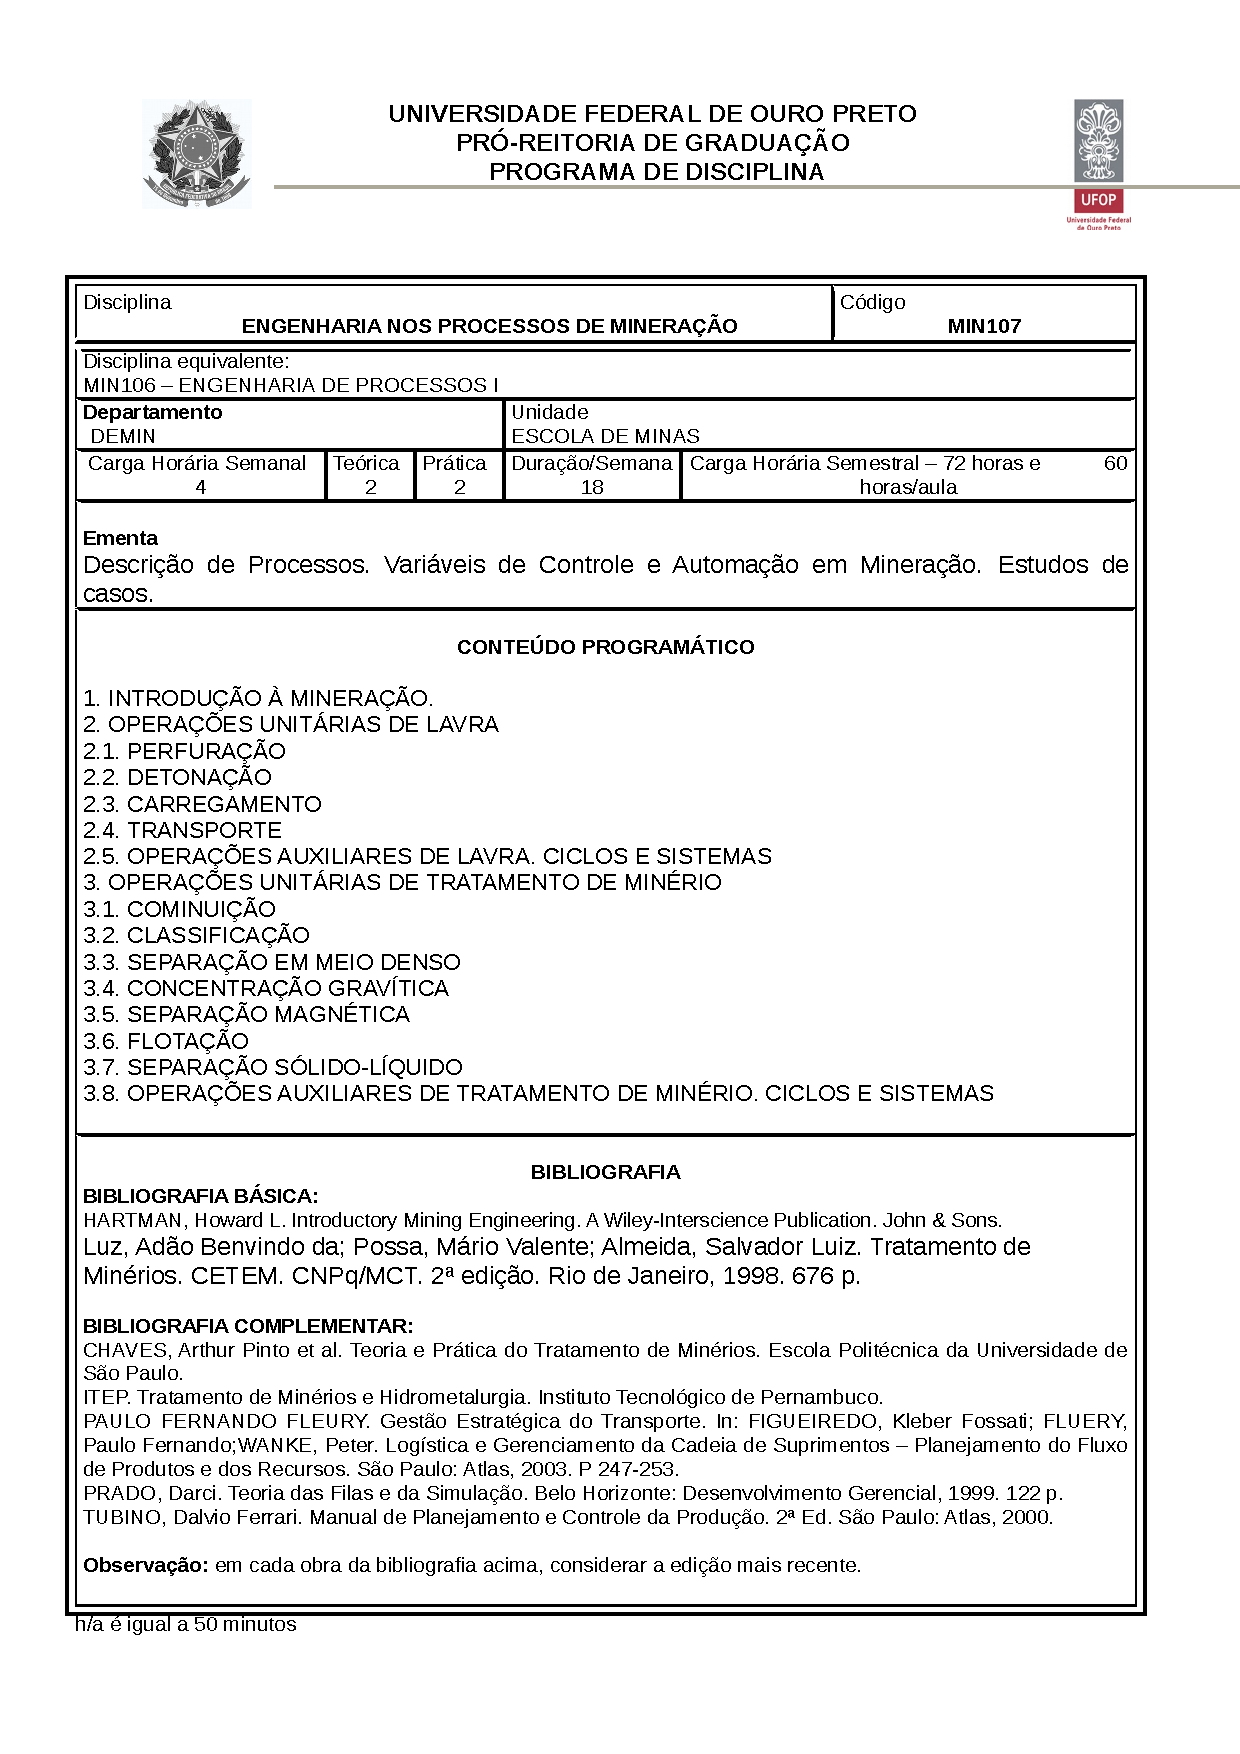
\includegraphics[scale=0.7]{capitulos/anexo1-programas-disciplina/p95.pdf}
	%	\caption{Disciplina do primeiro semestre}
\end{figure}

\begin{figure}[p]
	\centering 
	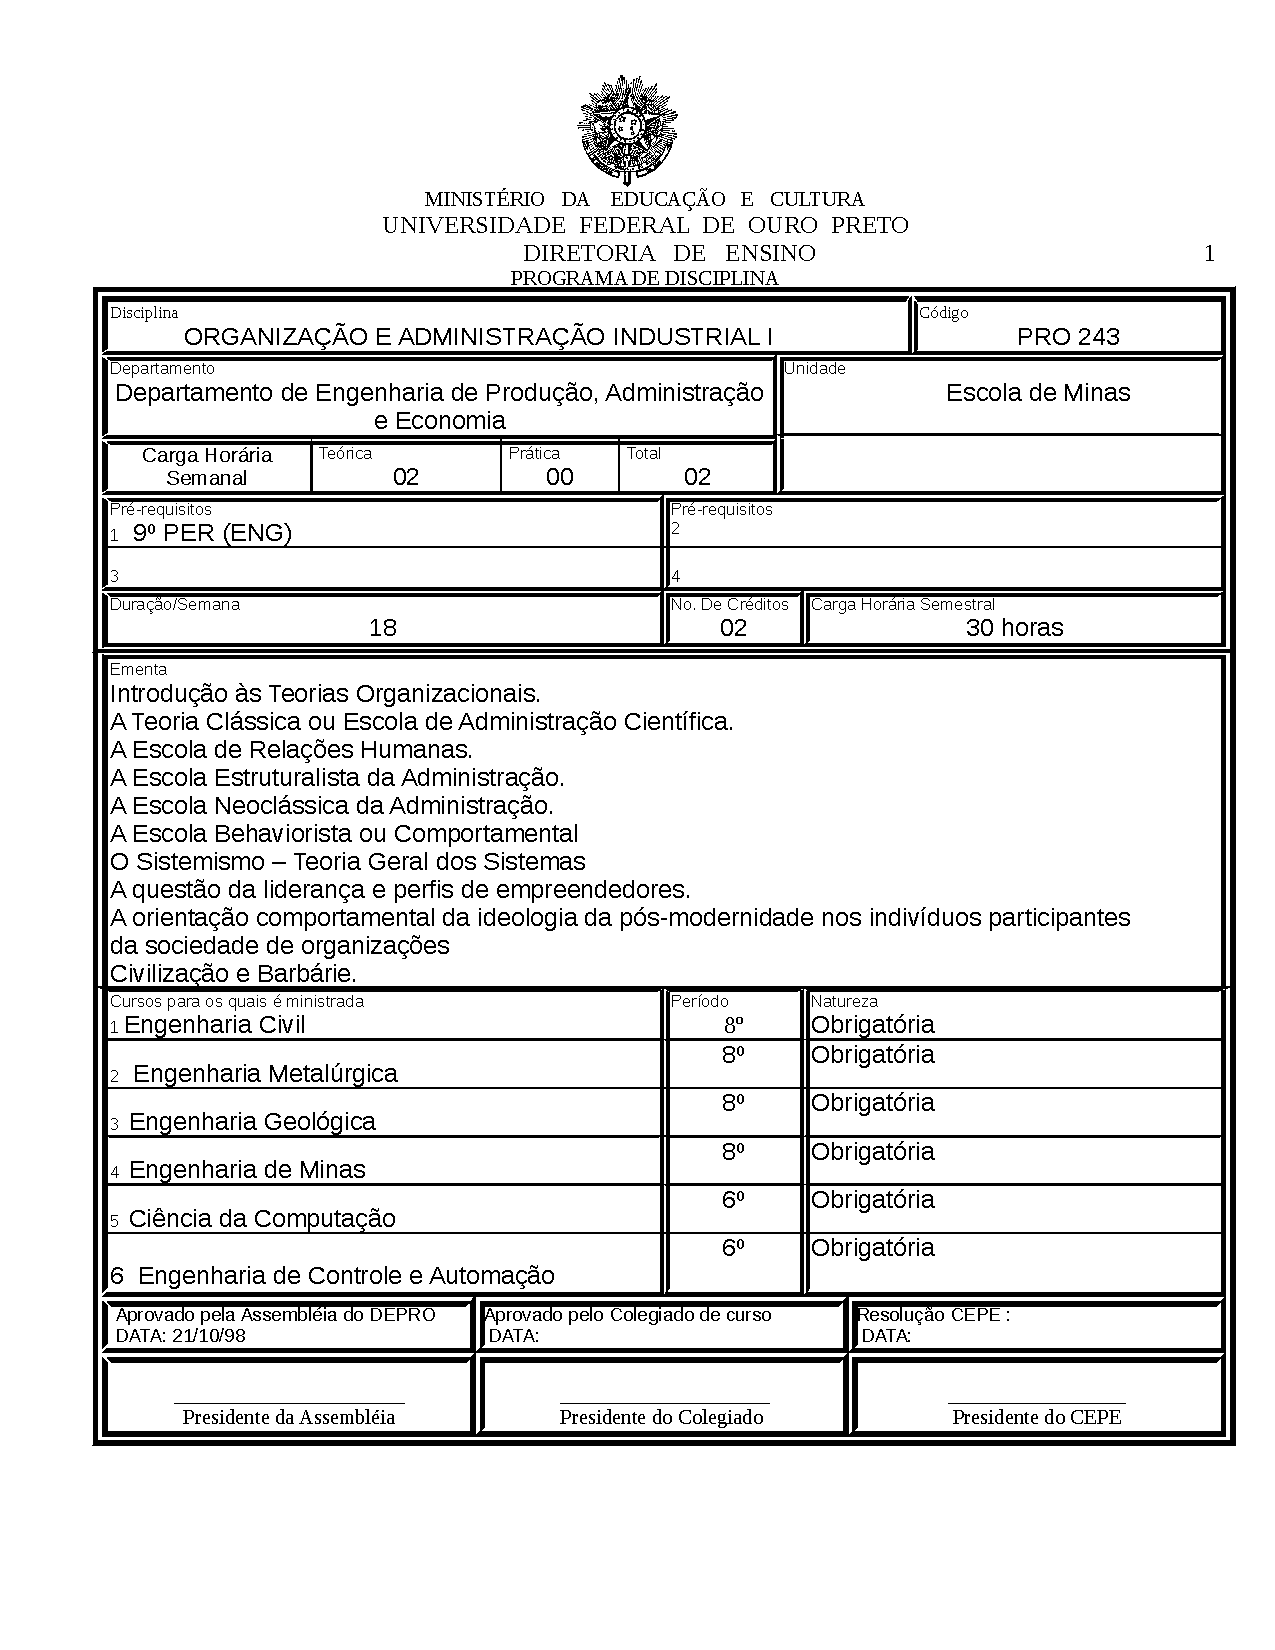
\includegraphics[scale=0.7]{capitulos/anexo1-programas-disciplina/p96.pdf}
	%	\caption{Disciplina do primeiro semestre}
\end{figure}

%Decimo semestre
\begin{figure}[p]
	\centering 
	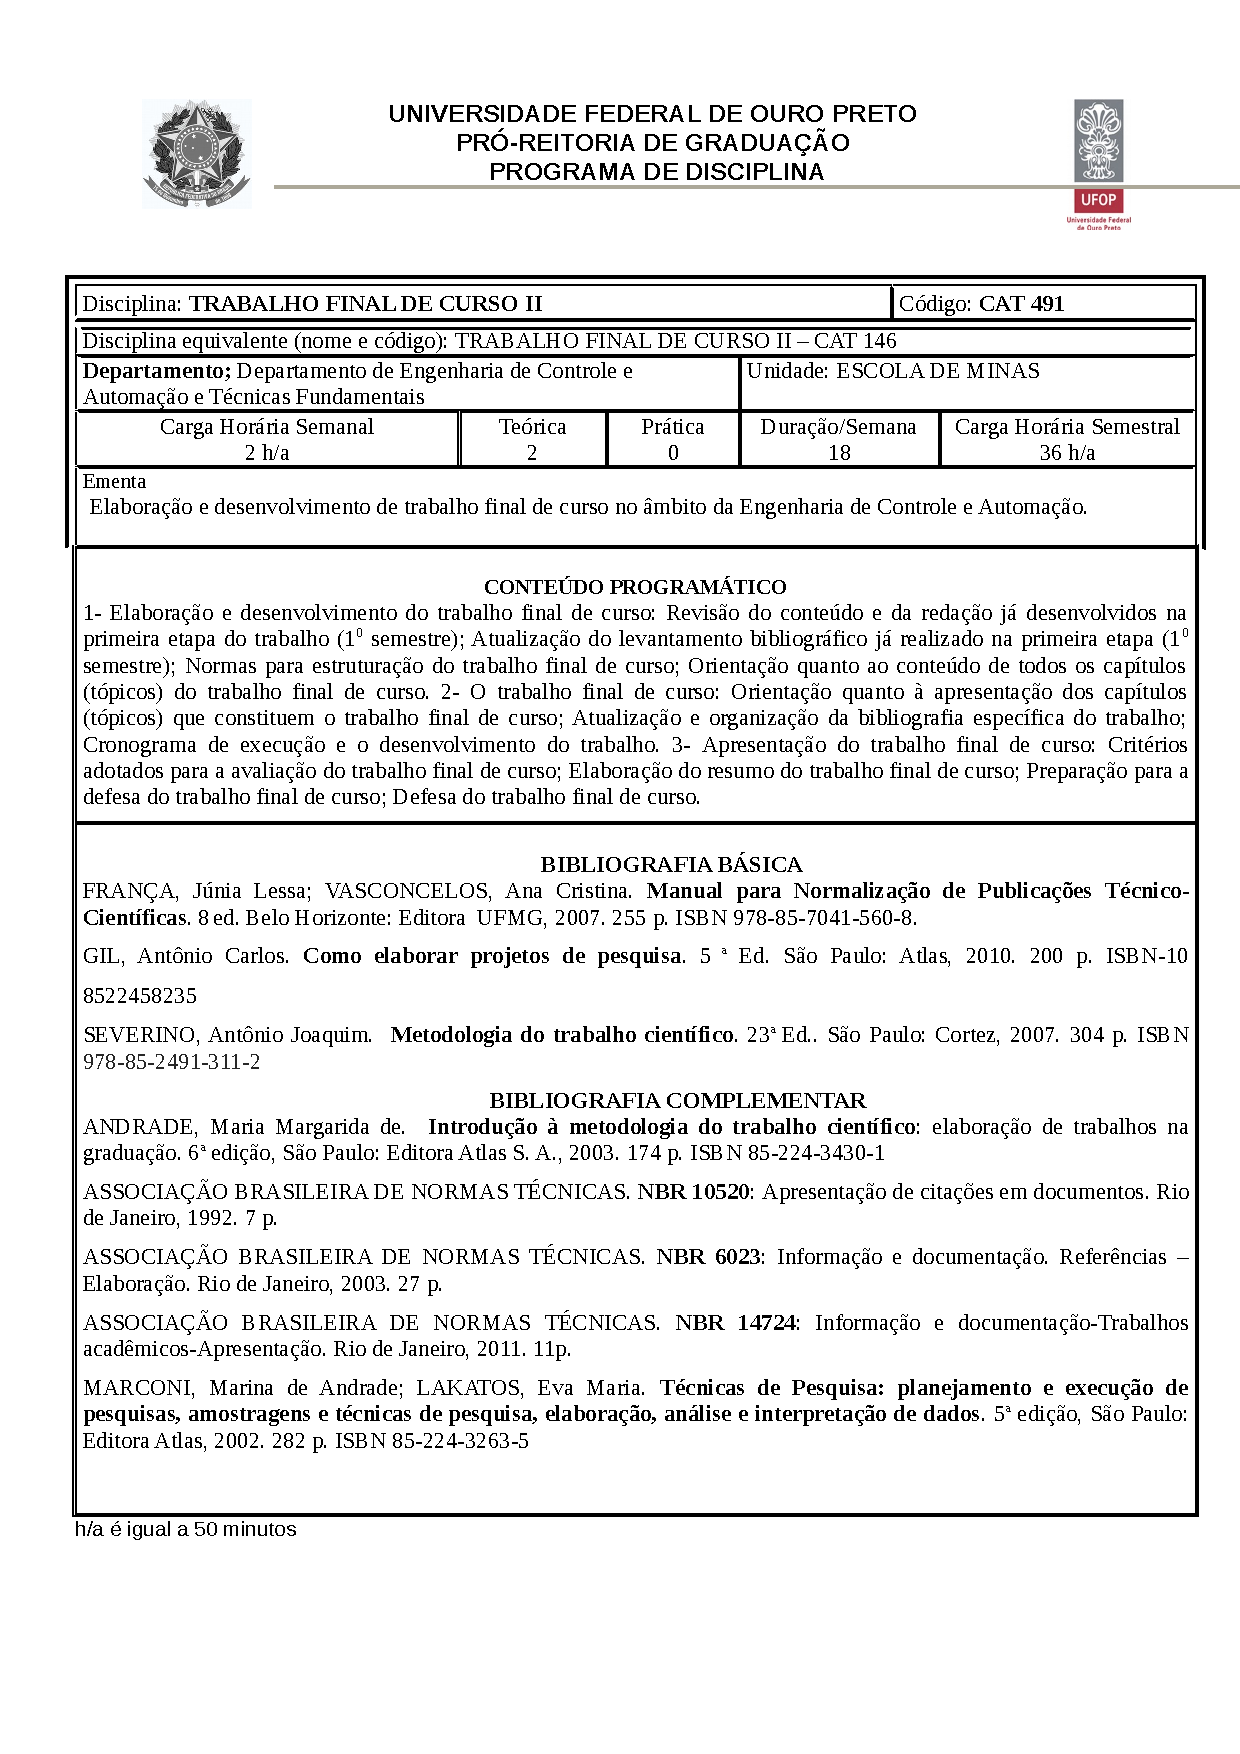
\includegraphics[scale=0.7]{capitulos/anexo1-programas-disciplina/p101.pdf}
	%	\caption{Disciplina do primeiro semestre}
\end{figure}

\begin{figure}[p]
	\centering 
	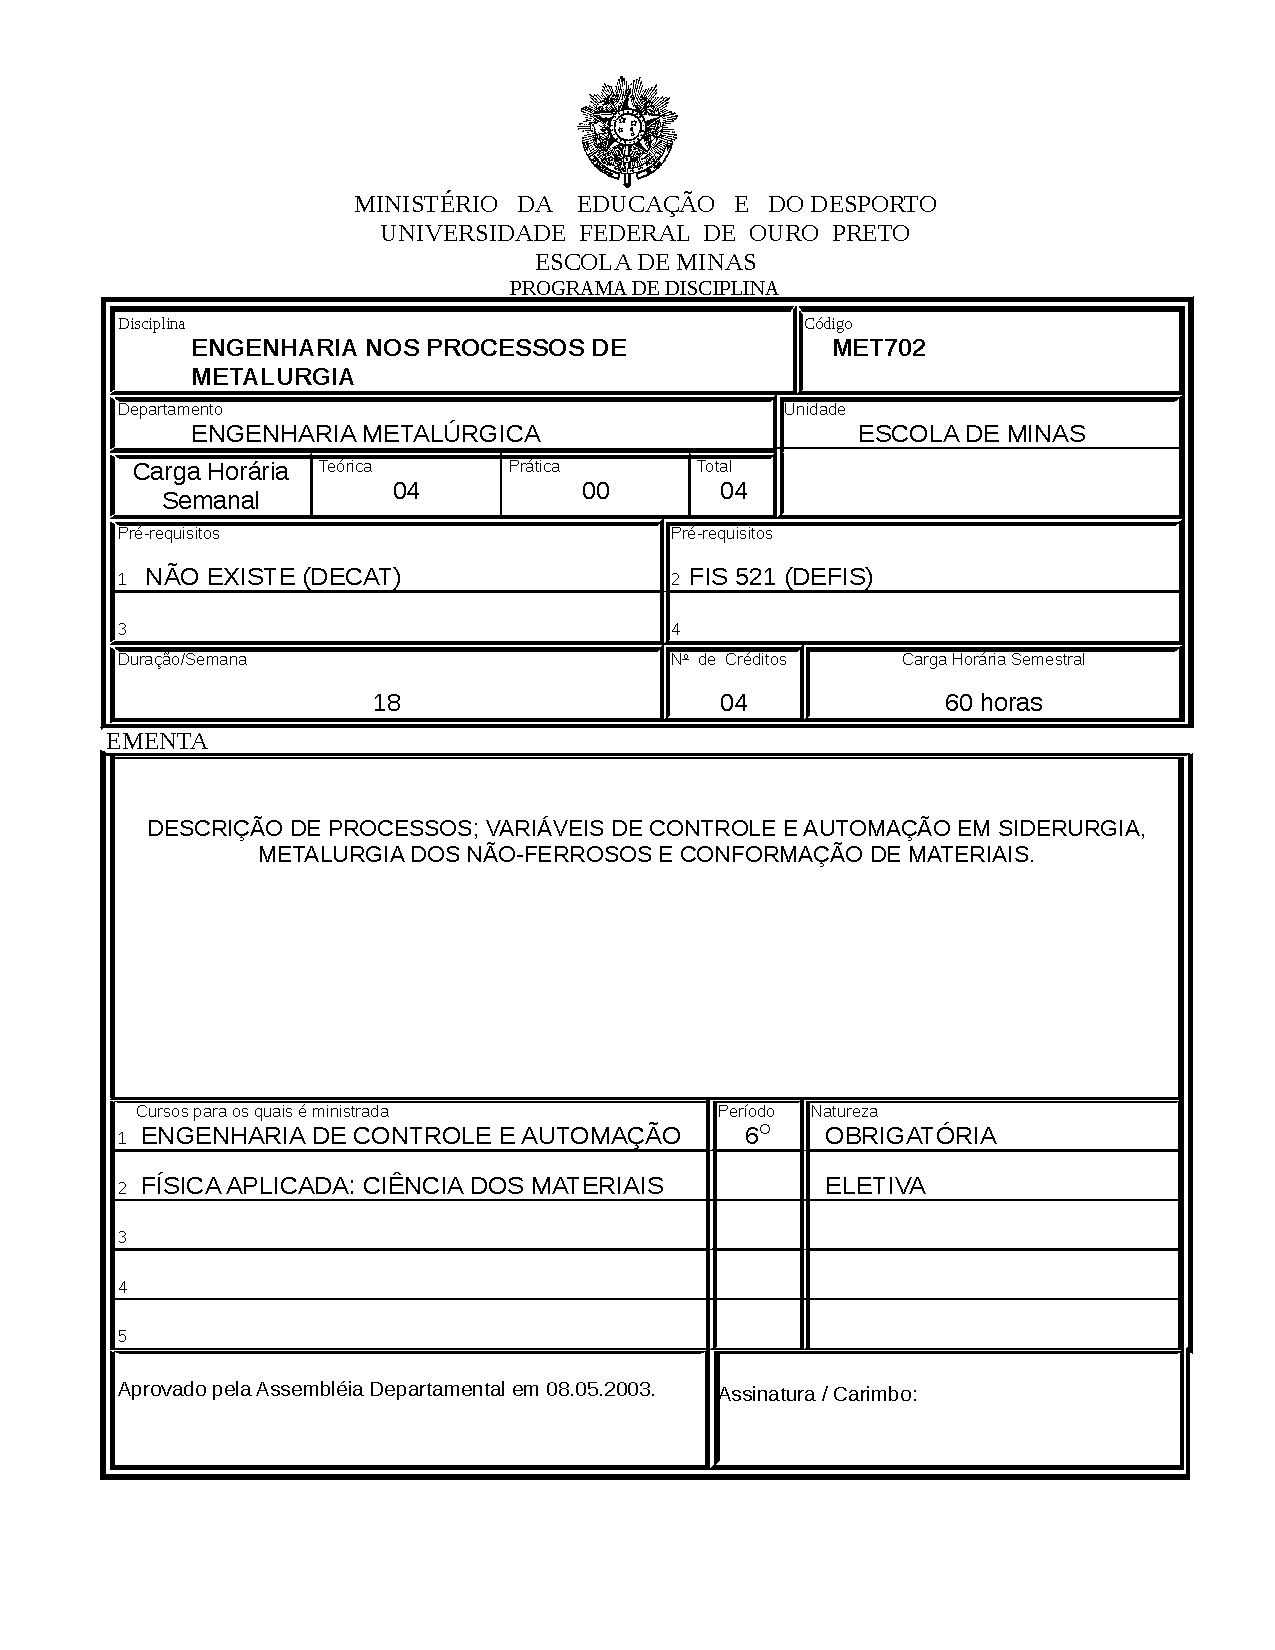
\includegraphics[scale=0.7]{capitulos/anexo1-programas-disciplina/p102.pdf}
	%	\caption{Disciplina do primeiro semestre}
\end{figure}

\begin{figure}[p]
	\centering 
	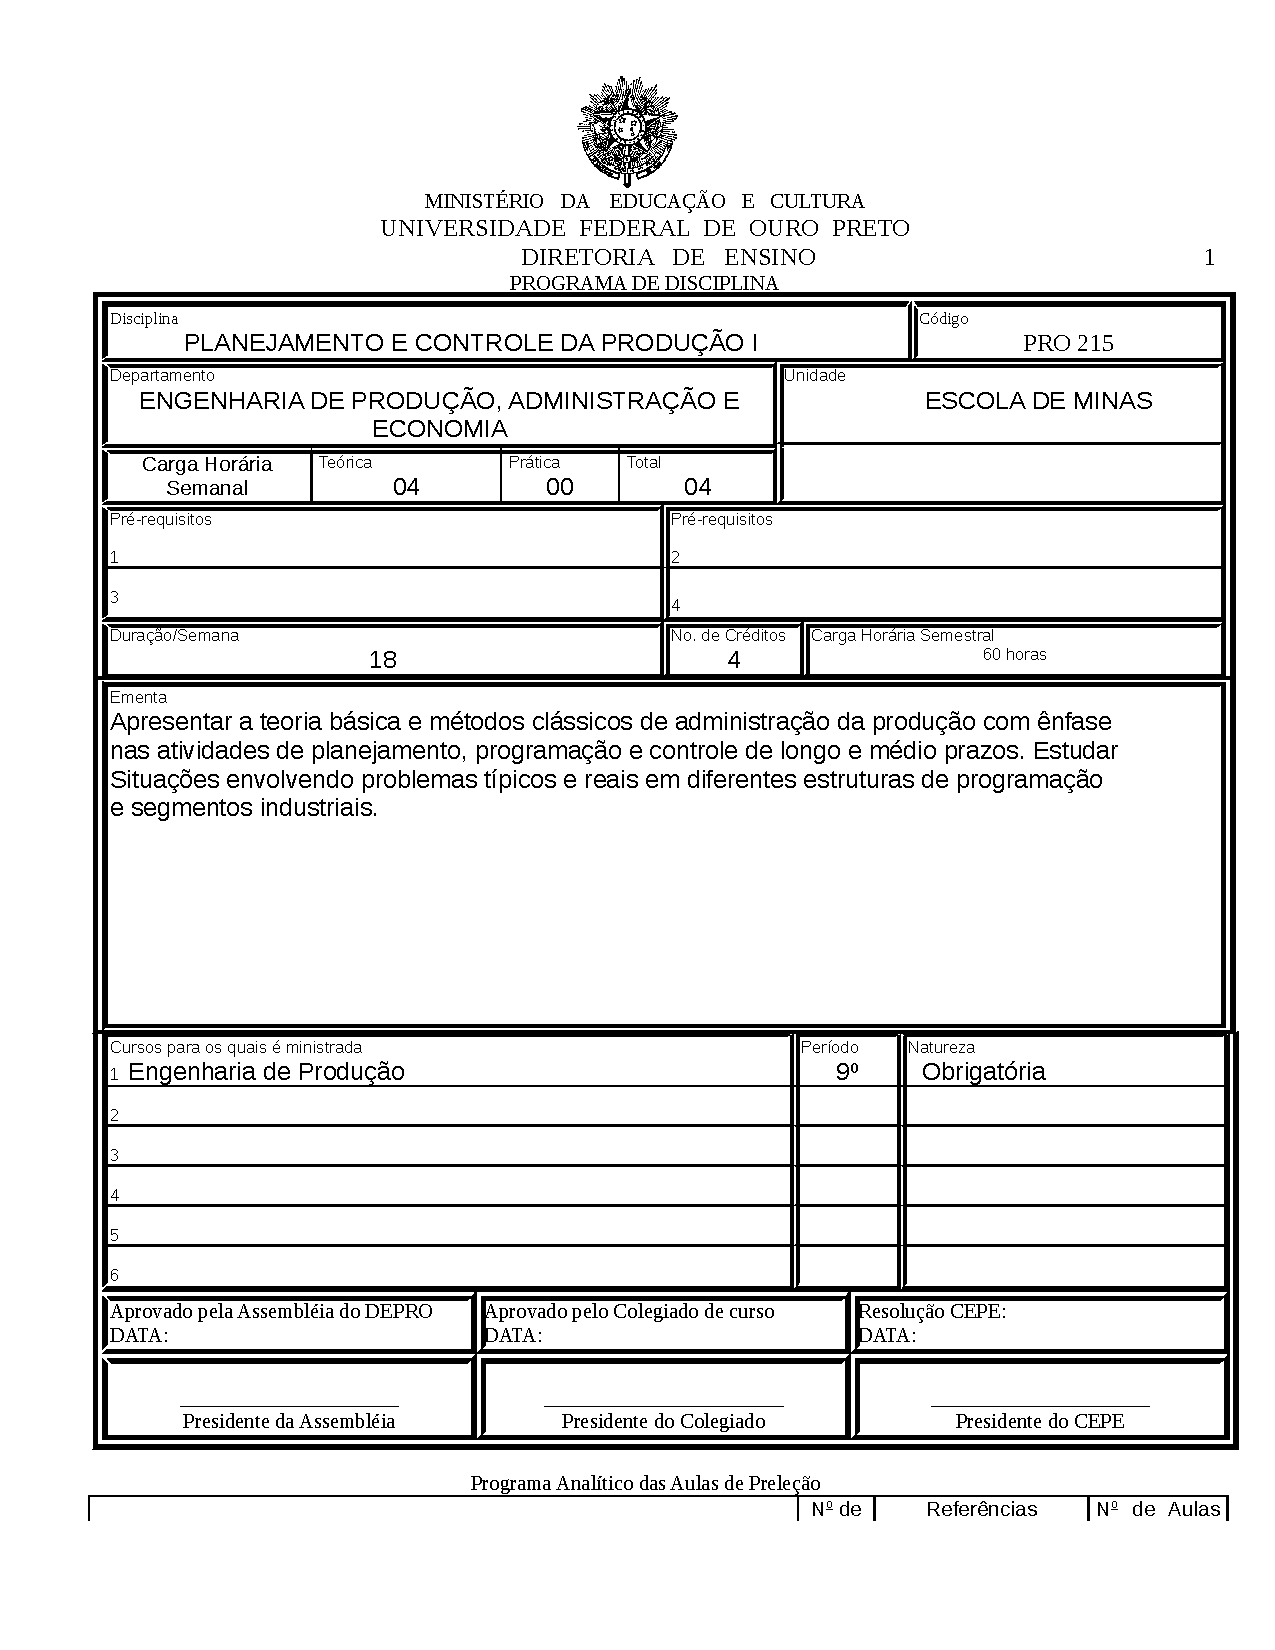
\includegraphics[scale=0.7]{capitulos/anexo1-programas-disciplina/p103.pdf}
	%	\caption{Disciplina do primeiro semestre}
\end{figure}
\pagebreak

\begin{figure}[p]
	\centering 
	\includegraphics[scale=0.7]{capitulos/anexo1-programas-disciplina/p104.pdf}
	%	\caption{Disciplina do primeiro semestre}
\end{figure}

% eletivas grupo 1
\begin{figure}[p]
	\centering 
	\includegraphics[scale=0.7]{capitulos/anexo1-programas-disciplina/eg11.pdf}
	%	\caption{Disciplina do primeiro semestre}
\end{figure}


\begin{figure}[p]
	\centering 
	\includegraphics[scale=0.7]{capitulos/anexo1-programas-disciplina/eg12.pdf}
	%	\caption{Disciplina do primeiro semestre}
\end{figure}

\begin{figure}[p]
	\centering 
	\includegraphics[scale=0.7]{capitulos/anexo1-programas-disciplina/eg13.pdf}
	%	\caption{Disciplina do primeiro semestre}
\end{figure}

\begin{figure}[p]
	\centering 
	\includegraphics[scale=0.7]{capitulos/anexo1-programas-disciplina/eg14.pdf}
	%	\caption{Disciplina do primeiro semestre}
\end{figure}

\begin{figure}[p]
	\centering 
	\includegraphics[scale=0.7]{capitulos/anexo1-programas-disciplina/eg15.pdf}
	%	\caption{Disciplina do primeiro semestre}
\end{figure}

\begin{figure}[p]
	\centering 
	\includegraphics[scale=0.7]{capitulos/anexo1-programas-disciplina/eg16.pdf}
	%	\caption{Disciplina do primeiro semestre}
\end{figure}

\begin{figure}[p]
	\centering 
	\includegraphics[scale=0.7]{capitulos/anexo1-programas-disciplina/eg17.pdf}
	%	\caption{Disciplina do primeiro semestre}
\end{figure}

\begin{figure}[p]
	\centering 
	\includegraphics[scale=0.7]{capitulos/anexo1-programas-disciplina/eg18.pdf}
	%	\caption{Disciplina do primeiro semestre}
\end{figure}

\begin{figure}[p]
	\centering 
	\includegraphics[scale=0.7]{capitulos/anexo1-programas-disciplina/eg19.pdf}
	%	\caption{Disciplina do primeiro semestre}
\end{figure}

%eletivas - grupo2

\begin{figure}[p]
	\centering 
	\includegraphics[scale=0.7]{capitulos/anexo1-programas-disciplina/eg21.pdf}
	%	\caption{Disciplina do primeiro semestre}
\end{figure}

\begin{figure}[p]
	\centering 
	\includegraphics[scale=0.7]{capitulos/anexo1-programas-disciplina/eg22.pdf}
	%	\caption{Disciplina do primeiro semestre}
\end{figure}

\begin{figure}[p]
	\centering 
	\includegraphics[scale=0.7]{capitulos/anexo1-programas-disciplina/eg23.pdf}
	%	\caption{Disciplina do primeiro semestre}
\end{figure}

\begin{figure}[p]
	\centering 
	\includegraphics[scale=0.7]{capitulos/anexo1-programas-disciplina/eg24.pdf}
	%	\caption{Disciplina do primeiro semestre}
\end{figure}

\begin{figure}[p]
	\centering 
	\includegraphics[scale=0.7]{capitulos/anexo1-programas-disciplina/eg25.pdf}
	%	\caption{Disciplina do primeiro semestre}
\end{figure}

% eletivas - grupo 3

\begin{figure}[p]
	\centering 
	\includegraphics[scale=0.7]{capitulos/anexo1-programas-disciplina/eg31.pdf}
	%	\caption{Disciplina do primeiro semestre}
\end{figure}

\begin{figure}[p]
	\centering 
	\includegraphics[scale=0.7]{capitulos/anexo1-programas-disciplina/eg32.pdf}
	%	\caption{Disciplina do primeiro semestre}
\end{figure}

\begin{figure}[p]
	\centering 
	\includegraphics[scale=0.7]{capitulos/anexo1-programas-disciplina/eg33.pdf}
	%	\caption{Disciplina do primeiro semestre}
\end{figure}

\begin{figure}[p]
	\centering 
	\includegraphics[scale=0.7]{capitulos/anexo1-programas-disciplina/eg34.pdf}
	%	\caption{Disciplina do primeiro semestre}
\end{figure}

\begin{figure}[p]
	\centering 
	\includegraphics[scale=0.7]{capitulos/anexo1-programas-disciplina/eg35.pdf}
	%	\caption{Disciplina do primeiro semestre}
\end{figure}

\begin{figure}[p]
	\centering 
	\includegraphics[scale=0.7]{capitulos/anexo1-programas-disciplina/eg36.pdf}
	%	\caption{Disciplina do primeiro semestre}
\end{figure}

\begin{figure}[p]
	\centering 
	\includegraphics[scale=0.7]{capitulos/anexo1-programas-disciplina/eg37.pdf}
	%	\caption{Disciplina do primeiro semestre}
\end{figure}

\begin{figure}[p]
	\centering 
	\includegraphics[scale=0.7]{capitulos/anexo1-programas-disciplina/eg38.pdf}
	%	\caption{Disciplina do primeiro semestre}
\end{figure}

\begin{figure}[p]
	\centering 
	\includegraphics[scale=0.7]{capitulos/anexo1-programas-disciplina/eg39.pdf}
	%	\caption{Disciplina do primeiro semestre}
\end{figure}

\begin{figure}[p]
	\centering 
	\includegraphics[scale=0.7]{capitulos/anexo1-programas-disciplina/eg310.pdf}
	%	\caption{Disciplina do primeiro semestre}
\end{figure}

\begin{figure}[p]
	\centering 
	\includegraphics[scale=0.7]{capitulos/anexo1-programas-disciplina/eg311.pdf}
	%	\caption{Disciplina do primeiro semestre}
\end{figure}

\begin{figure}[p]
	\centering 
	\includegraphics[scale=0.7]{capitulos/anexo1-programas-disciplina/eg312.pdf}
	%	\caption{Disciplina do primeiro semestre}
\end{figure}

\begin{figure}[p]
	\centering 
	\includegraphics[scale=0.7]{capitulos/anexo1-programas-disciplina/eg313.pdf}
	%	\caption{Disciplina do primeiro semestre}
\end{figure}

\begin{figure}[p]
	\centering 
	\includegraphics[scale=0.7]{capitulos/anexo1-programas-disciplina/eg314.pdf}
	%	\caption{Disciplina do primeiro semestre}
\end{figure}

\begin{figure}[p]
	\centering 
	\includegraphics[scale=0.7]{capitulos/anexo1-programas-disciplina/eg315.pdf}
	%	\caption{Disciplina do primeiro semestre}
\end{figure}

\begin{figure}[p]
	\centering 
	\includegraphics[scale=0.7]{capitulos/anexo1-programas-disciplina/eg316.pdf}
	%	\caption{Disciplina do primeiro semestre}
\end{figure}

\begin{figure}[p]
	\centering 
	\includegraphics[scale=0.7]{capitulos/anexo1-programas-disciplina/eg317.pdf}
	%	\caption{Disciplina do primeiro semestre}
\end{figure}

\begin{figure}[p]
	\centering 
	\includegraphics[scale=0.7]{capitulos/anexo1-programas-disciplina/eg318.pdf}
	%	\caption{Disciplina do primeiro semestre}
\end{figure}

\begin{figure}[p]
	\centering 
	\includegraphics[scale=0.7]{capitulos/anexo1-programas-disciplina/eg319.pdf}
	%	\caption{Disciplina do primeiro semestre}
\end{figure}

\begin{figure}[p]
	\centering 
	\includegraphics[scale=0.7]{capitulos/anexo1-programas-disciplina/eg320.pdf}
	%	\caption{Disciplina do primeiro semestre}
\end{figure}

\begin{figure}[p]
	\centering 
	\includegraphics[scale=0.7]{capitulos/anexo1-programas-disciplina/eg321.pdf}
	%	\caption{Disciplina do primeiro semestre}
\end{figure}

\chapter{Resoluções CEPE} 
\label{ape:02} \index{matriz-curricular}
%cepe 2088
\begin{figure}[p]
	\centering 
	\includegraphics[scale=0.7]{capitulos/resolucoes-cepe/cepe2088.pdf}
	%	\caption{Disciplina do primeiro semestre}
\end{figure}

%cepe1586
\begin{figure}[p]
	\centering 
	\includegraphics[scale=0.7]{capitulos/resolucoes-cepe/cepe1586-p1.pdf}
	%	\caption{Disciplina do primeiro semestre}
\end{figure}

\begin{figure}[p]
	\centering 
	\includegraphics[scale=0.7]{capitulos/resolucoes-cepe/cepe1586-p2.pdf}
	%	\caption{Disciplina do primeiro semestre}
\end{figure}

%cepe1681
\begin{figure}[p]
	\centering 
	\includegraphics[scale=0.7]{capitulos/resolucoes-cepe/cepe1681-p1.pdf}
	%	\caption{Disciplina do primeiro semestre}
\end{figure}

\begin{figure}[p]
	\centering 
	\includegraphics[scale=0.7]{capitulos/resolucoes-cepe/cepe1681-p2.pdf}
	%	\caption{Disciplina do primeiro semestre}
\end{figure}
\chapter{Modelo de programa de disciplina} 
\label{ape:03} \index{template-programa-disciplina}
%
%modelo de programa
\begin{figure}[p]
	\centering 
	\includegraphics[scale=0.7]{capitulos/modelo-programa/pdp1.pdf}
\end{figure}

\begin{figure}[p]
	\centering 
	\includegraphics[scale=0.7]{capitulos/modelo-programa/pdp2.pdf}
\end{figure}

\begin{figure}[p]
	\centering 
	\includegraphics[scale=0.7]{capitulos/modelo-programa/pdp3.pdf}
\end{figure}
\chapter[Plano de integraliza{\c c}{\~a}o]{Plano de integraliza{\c c}{\~a}o da carga hor{\'a}ria do curso} 
\label{ape:04} \index{plano-integralizacao}
%
Texto do anexo \ref{ape:04}.
\end{apendicesenv}
% ---

% ----------------------------------------------------------
% Anexos
% ----------------------------------------------------------
%(Lembre-se: Apendices são de autoria do próprio autor do texto. 
% Anexos são elementos de autorias de outros, que o autor do texto julga interessante apresentar)
% ---
% Inicia os anexos
% ---
\begin{anexosenv}

% Imprime uma página indicando o início dos anexos
\partanexos
% ---
% Insere arquivo com os anexos 1, 2 e 3
% ---
\end{anexosenv}

%---------------------------------------------------------------------
% INDICE REMISSIVO
%---------------------------------------------------------------------
%\phantompart
\printindex
%---------------------------------------------------------------------

\end{document}
